%%%%%%%%%%%%%%%%%%%%%%%%%%%%%%%%%%%%%%%%%%%%%%%%%%%%%%%%%%%

%% document class
\documentclass[a4paper,12pt,oneside]{report}

% latex template: https://www.overleaf.com/project/5e7ca0498eb4030001ac3e0c
%% packages
\usepackage[left=2.5cm,right=2.5cm,top=2cm,bottom=2cm]{geometry}
\newcommand{\myparagraph}[1]{\textbf{#1}\mbox{}\\} % next line after paragraph use
\newcommand{\boldheader}[1]{\vspace{0.5cm}\textbf{#1}\mbox{}\\} % bold header titles and space before and after
\newcommand{\underlineheader}[1]{\vspace{0.5cm}\underline{#1}\mbox{}\\} % bold header titles and space before and after
\newcommand*\conj[1]{\bar{#1}}
\newenvironment{changemargin}[1]{\begin{list}{}{\setlength{\voffset}{#1}}\item[]}{\end{list}} %change margin for long table intro
\def\checkmark{\tikz\fill[scale=0.4](0,.35) -- (.25,0) -- (1,.7) -- (.25,.15) -- cycle;} 

\usepackage{graphicx}
\usepackage{verbatim}
\usepackage{latexsym}
%\usepackage{mathchars}
\usepackage{setspace}
\usepackage{subfiles}
\usepackage[parfill]{parskip}
\usepackage{siunitx,tabularx,ragged2e,booktabs,caption,multirow}
\usepackage{tocloft} % local contents list 
\usepackage{etoc} % local contents list 
\setcounter{secnumdepth}{4} % local contents list 
\usepackage{etoolbox} % https://tex.stackexchange.com/questions/384514/make-subsection-visible-in-local-toc-only-not-in-main-toc
\usepackage[titletoc,page, title, header]{appendix}
\usepackage{enumitem} % enumerate, itemize formatting
%\immediate\write18{makeindex \Knit.nlo -s nomencl.ist -o Knit.nls} 
\usepackage{nomencl} %list of abbreviations
\makenomenclature
\setlength{\nomlabelwidth}{2.5cm}
\setlength{\nomitemsep}{-\parsep}
\usepackage{xr} % for cross-referencing of chapters
\usepackage{ulem} % underline
\usepackage[T1]{fontenc} % underscore
\usepackage{subcaption} % multiple figures 
\usepackage[dvipsnames,table]{xcolor} % colour text
\usepackage{libertine} % space between text on same line
\usepackage{amsmath} % maths equation alignment 
\usepackage[euler]{textgreek} % greek letters
\usepackage{tikz} %tick mark
\usepackage{pdfpages} % import pdf s
\usepackage{pdflscape} %landscape pdf

%% Bibliography
\usepackage[superscript,biblabel]{cite}
%\usepackage[round]{natbib} % referecing style with ()
%\bibliographystyle{plainnat} % bioligraophy 

\AtBeginEnvironment{appendix}{\etocsettocdepth.toc{section}\etocignoretoctocdepth
	\etocsetnexttocdepth{subsection}}

% tables and landscape
\captionsetup[table]{width=16cm}
\usepackage{booktabs}
\usepackage{multirow}
\usepackage{lscape}
\usepackage{todonotes} %todonotes
\usepackage{longtable} % longtables overflow into next page
\usepackage{array} %table
\usepackage{tablefootnote} %tablefoonote
\usepackage{threeparttable} %table
\usepackage{arydshln} %dash line
\setlength{\LTcapwidth}{10.2in} %width of long table caption
\newcommand{\tabitem}{\textbullet~~}

\usepackage{notoccite}
\usepackage{hyperref} %hyperlinks
\hypersetup{
	colorlinks=true, %set true if you want colored links
	linktoc=all,     %set to all if you want both sections and subsections linked
	linkcolor=black,  %choose some color if you want links to stand out
	citecolor=black,
	urlcolor=black
}

\usepackage[capitalize, nameinlink]{cleveref}
\crefdefaultlabelformat{#2\textbf{#1}#3} % <-- Only #1 in \textbf
\crefname{section}{\textbf{Section}}{\textbf{Sections}}
\crefname{chapter}{\textbf{Chapter}}{\textbf{Chapter}}
\crefname{table}{\textbf{Table}}{\textbf{Table}}
\crefname{figure}{\textbf{Figure}}{\textbf{Figure}}
%\Crefname{section}{\textbf{Section}}{\textbf{Sections}}



\input{code.sty} % for including programming 
%\setlength{\parskip}{5*\lineskip}  % a little space before a \par
%\setlength{\parindent}{0pt}	      % don't indent first lines of paragraphs
\input{uhead.sty}
\input{boxit.sty}
% Created by Yue Li, June 2017

\pagestyle{empty}

\setlength{\parskip}{1.5em}
%\setlength{\parindent}{0em}
\setlength\itemsep{-0.5em}
\newlength\tocrulewidth
\setlength{\tocrulewidth}{1.5pt}
\setenumerate{itemsep=-1.5em,topsep=-1.5em}
\setitemize{itemsep=-1.5em,topsep=-1.5em}
\usepackage[width=0.8\textwidth, labelfont=bf]{caption}

\makeatletter  %to avoid error messages generated by "\@". Makes Latex treat "@" like a letter

\linespread{1.5}
\def\submitdate#1{\gdef\@submitdate{#1}}
\def\degree#1{\gdef\@degree{#1}}
\def\studentid#1{\gdef\@studentid{#1}}
\def\supervisor#1{\gdef\@supervisor{#1}}

\def\titlepage{
  \newpage
  \centering
  \linespread{1}
  \normalsize
  \vbox to \vsize\bgroup\vbox to 9in\bgroup
}
\def\endtitlepage{
  \par
  \kern 0pt
  \egroup
  \vss
  \egroup
  \cleardoublepage
}

\def\abstract{
  \begin{center}{
    \large\bf Abstract}
  \end{center}
  \small
  %\def\baselinestretch{1.5}
  \linespread{1.5}
  \normalsize
}
\def\endabstract{
  \par
}

\newenvironment{acknowledgements}{
  \cleardoublepage
  \begin{center}{
    \large \bf Acknowledgements}
  \end{center}
  \small
  \linespread{1.5}
  \normalsize
}{\cleardoublepage}
\def\endacknowledgements{
  \par
}

\def\preface{
    \pagenumbering{roman}
    \pagestyle{plain}
    \doublespacing
}

\def\body{
	
    \cleardoublepage    
    \pagestyle{uheadings}
    \tableofcontents
    \pagestyle{plain}
    \cleardoublepage
    \pagestyle{uheadings}
    \listoftables
    \pagestyle{plain}
    \cleardoublepage
    \pagestyle{uheadings}
    \listoffigures
    \pagestyle{plain}
    \cleardoublepage
    \pagestyle{uheadings}
    \pagenumbering{arabic}
    \doublespacing
    
}

\makeatother  %to avoid error messages generated by "\@". Makes Latex treat "@" like a letter

\lstset{style=mystyle}

\newcommand{\spacetable}{\vspace{3cm}} % function for "\spacetable"
\newcommand{\ipc}{{\sf ipc}}

\DeclareCaptionType{myequation}[][List of equations] %equations
\captionsetup[myequation]{labelformat=simple, name=Equation, labelsep=colon} %equations

% https://tex.stackexchange.com/questions/95838/how-to-write-a-perfect-equation-parameters-description
\newenvironment{conditions*}
{\par\vspace{\abovedisplayskip}\noindent
	\tabularx{\columnwidth}{>{$}l<{$} @{${}={}$} >{\raggedright\arraybackslash}X}}
{\endtabularx\par\vspace{\belowdisplayskip}}

\newcommand{\Prob}{\bbbp}
\newcommand{\Real}{\bbbr}
\newcommand{\real}{\Real}
\newcommand{\Int}{\bbbz}
\newcommand{\Nat}{\bbbn}

\newcommand{\NN}{{\sf I\kern-0.14emN}}   % Natural numbers
\newcommand{\ZZ}{{\sf Z\kern-0.45emZ}}   % Integers
\newcommand{\QQQ}{{\sf C\kern-0.48emQ}}   % Rational numbers
\newcommand{\RR}{{\sf I\kern-0.14emR}}   % Real numbers
\newcommand{\KK}{{\cal K}}
\newcommand{\OO}{{\cal O}}
\newcommand{\AAA}{{\bf A}}
\newcommand{\HH}{{\bf H}}
\newcommand{\II}{{\bf I}}
\newcommand{\LL}{{\bf L}}
\newcommand{\PP}{{\bf P}}
\newcommand{\PPprime}{{\bf P'}}
\newcommand{\QQ}{{\bf Q}}
\newcommand{\UU}{{\bf U}}
\newcommand{\UUprime}{{\bf U'}}
\newcommand{\zzero}{{\bf 0}}
\newcommand{\ppi}{\mbox{\boldmath $\pi$}}
\newcommand{\aalph}{\mbox{\boldmath $\alpha$}}
\newcommand{\bb}{{\bf b}}
\newcommand{\ee}{{\bf e}}
\newcommand{\mmu}{\mbox{\boldmath $\mu$}}
\newcommand{\vv}{{\bf v}}
\newcommand{\xx}{{\bf x}}
\newcommand{\yy}{{\bf y}}
\newcommand{\zz}{{\bf z}}
\newcommand{\oomeg}{\mbox{\boldmath $\omega$}}
\newcommand{\res}{{\bf res}}
\newcommand{\cchi}{{\mbox{\raisebox{.4ex}{$\chi$}}}}
%\newcommand{\cchi}{{\cal X}}
%\newcommand{\cchi}{\mbox{\Large $\chi$}}

% Logical operators and symbols
\newcommand{\imply}{\Rightarrow}
\newcommand{\bimply}{\Leftrightarrow}
\newcommand{\union}{\cup}
\newcommand{\intersect}{\cap}
\newcommand{\boolor}{\vee}
\newcommand{\booland}{\wedge}
\newcommand{\boolimply}{\imply}
\newcommand{\boolbimply}{\bimply}
\newcommand{\boolnot}{\neg}
\newcommand{\boolsat}{\!\models}
\newcommand{\boolnsat}{\!\not\models}


\newcommand{\op}[1]{\mathrm{#1}}
\newcommand{\s}[1]{\ensuremath{\mathcal #1}}

% Properly styled differentiation and integration operators
\newcommand{\diff}[1]{\mathrm{\frac{d}{d\mathit{#1}}}}
\newcommand{\diffII}[1]{\mathrm{\frac{d^2}{d\mathit{#1}^2}}}
\newcommand{\intg}[4]{\int_{#3}^{#4} #1 \, \mathrm{d}#2}
\newcommand{\intgd}[4]{\int\!\!\!\!\int_{#4} #1 \, \mathrm{d}#2 \, \mathrm{d}#3}

% Large () brackets on different lines of an eqnarray environment
\newcommand{\Leftbrace}[1]{\left(\raisebox{0mm}[#1][#1]{}\right.}
\newcommand{\Rightbrace}[1]{\left.\raisebox{0mm}[#1][#1]{}\right)}

% Funky symobols for footnotes
\newcommand{\symbolfootnote}{\renewcommand{\thefootnote}{\fnsymbol{footnote}}}
% now add \symbolfootnote to the beginning of the document...

\newcommand{\normallinespacing}{\renewcommand{\baselinestretch}{1.5} \normalsize}
\newcommand{\mediumlinespacing}{\renewcommand{\baselinestretch}{1.2} \normalsize}
\newcommand{\narrowlinespacing}{\renewcommand{\baselinestretch}{1.0} \normalsize}
\newcommand{\bump}{\noalign{\vspace*{\doublerulesep}}}
\newcommand{\cell}{\multicolumn{1}{}{}}
\newcommand{\spann}{\mbox{span}}
\newcommand{\diagg}{\mbox{diag}}
\newcommand{\modd}{\mbox{mod}}
\newcommand{\minn}{\mbox{min}}
\newcommand{\andd}{\mbox{and}}
\newcommand{\forr}{\mbox{for}}
\newcommand{\EE}{\mbox{E}}

\newcommand{\deff}{\stackrel{\mathrm{def}}{=}}
\newcommand{\syncc}{~\stackrel{\textstyle \rhd\kern-0.57em\lhd}{\scriptstyle L}~}

\def\coop{\mbox{\large $\rhd\!\!\!\lhd$}}
\newcommand{\sync}[1]{\raisebox{-1.0ex}{$\;\stackrel{\coop}{\scriptscriptstyle
#1}\,$}}

\newtheorem{definition}{Definition}[chapter]
\newtheorem{theorem}{Theorem}[chapter]

\newcommand{\Figref}[1]{Figure~\ref{#1}}
\newcommand{\fig}[3]{
 \begin{figure}[!ht]
 \begin{center}
 \scalebox{#3}{\includegraphics{figs/#1.ps}}
 \vspace{-0.1in}
 \caption[ ]{\label{#1} #2}
 \end{center}
 \end{figure}
}

\newcommand{\figtwo}[8]{
 \begin{figure}
 \parbox[b]{#4 \textwidth}{
 \begin{center}
 \scalebox{#3}{\includegraphics{figs/#1.ps}}
 \vspace{-0.1in}
 \caption{\label{#1}#2}
 \end{center}
 }
 \hfill
 \parbox[b]{#8 \textwidth}{
 \begin{center}
 \scalebox{#7}{\includegraphics{figs/#5.ps}}
 \vspace{-0.1in}
 \caption{\label{#5}#6}
 \end{center}
 }
 \end{figure}
}
%\renewcommand{\nomname}{List of Abbreviations}

%% page settings
% Make the "Part I" text invisible
\renewcommand \thepart{}
\renewcommand \partname{}
\setlist[itemize]{noitemsep, topsep=-12pt} % space before itemise and paragraph
\setlist[enumerate]{noitemsep, topsep=-12pt} % space before itemise and paragraph



%%%%%%%%%%%%%%%%%%%%%%%%%%%%%%%%%%%%%%%%%%%%%%%%%%%%%%%%%%%

%==========================================================================================
%------------------------------------------------------------------------------------------
% Preamble 
%------------------------------------------------------------------------------------------

\begin{document}
\begin{minipage}[t]{\textwidth}
	\centering\large
	University of Exeter
	\par Department of Medical Sciences
\end{minipage}
\vskip 5em
\begin{center}
	{\noindent\LARGE \textbf{Genomic characterisation of Alzheimer's disease risk genes using long-read sequencing} \par}
	\vskip 1em
	{\Large 
		\begin{tabular}[t]{c}
			Szi Kay Leung
		\end{tabular}\par}
	\Large April, 2022
	%\vskip \z@ \@plus3fill
	\vskip 6em
	{\large Supervised by Professor Jonathan Mill, Dr Eilis Hannon, Dr Aaron Jeffries \& Professor David Collier \par}
	\vskip 1em
\end{center}

\begin{minipage}[b]{\textwidth}
	%\centering
	Submitted by Szi Kay Leung to the University of Exeter
	as a thesis for the degree of Doctor of Philosophy in Medical Sciences in April 2022.\\
	\\
	This thesis is available for Library use on the understanding that it
	is copyright material and that no quotation from the thesis may be published
	without proper acknowledgement.\\
	\\
	I certify that all material in this thesis which is not my own work has
	been identified and that no material has previously been submitted and
	approved for the award of a degree by this or any other University.\\
	\\
	\begin{flushright}(signature) .................................................................................................\end{flushright}
\end{minipage}
	





\begin{sloppypar}
\pagestyle{plain} % page numbering
\pagenumbering{gobble}
\begin{abstract}

Alzheimer's disease is a devastating neurodegenerative disorder characterised by progressive intracellular accumulation of hyperphosphorylated tau and extracellular deposition of amyloid-beta. It affects over 50 million people worldwide with numbers expecting to triple by 2050. Despite recent success in identifying genetic risk factors for AD, the mechanisms underpinning disease progression remain unknown. There is increasing evidence for altered transcriptional regulation and RNA splicing in the development of AD pathology. However, current studies exploring isoform diversity in the AD brain are constrained by the inherent limitations of standard short-read RNA-sequencing approaches, which fail to capture full-length transcripts critical for transcriptome assembly.  

The primary aim of this thesis was to utilise two long-read sequencing approaches, Pacific Biosciences isoform sequencing and Oxford Nanopore Technologies nanopore cDNA sequencing, to examine isoform diversity and transcript usage in the cortex, and identify alternative splicing events associated with AD pathology in a transgenic model of tau pathology (rTg4510). By generating long reads that span full-length transcripts, our studies revealed widespread RNA isoform diversity with unprecedented detection of novel transcripts not present in existing genome annotations. We further performed ultra-deep targeted long-read sequencing of 20 AD-risk genes, identifying robust expression changes at the transcript level associated with tau accumulation in the cortex. Our analyses provide a systematic evaluation of transcript usage, even in the absence of gene-level expression alterations, and highlight the importance of alternative RNA splicing as a mechanism underpinning gene regulation in the development of tau pathology. 

Finally, this thesis presents a laboratory and bioinformatics pipeline for the systematic analysis of isoform diversity and alternative splicing using long-read sequencing. The data generated as part of this research have implications for our understanding of the mechanisms driving the development of tau pathology, and represent a valuable resource to the wider research community.

\end{abstract}
\vspace*{\fill}
\centerline{\textit{To my fiancé, Tim}}
\vspace*{\fill}
\chapter*{Acknowledgements}

\begingroup
\singlespacing
While I had been warned of the difficulties of undertaking a PhD, I never would have imagined just how challenging and mentally taxing it could be. However, I have been blessed with the support of a number of people who have made this journey significantly easier and memorable. 

I would like to begin by thanking my supervisors – Professor Jonathan Mill, Dr Eilis Hannon and Dr Aaron Jeffries - for their invaluable guidance, patience and support throughout these four and a half years. Jon, thank you for the countless hours that you have spent patiently advising me throughout this PhD, and for always being so encouraging and enthusiastic about my results (even when I doubted them myself). Eilis, thank you for your insightful feedback and comments, and for being the person I could always turn to for a second, unbiased opinion. Aaron, thank you so much for sharing your invaluable expertise and knowledge be it in the lab or in bioinformatics, and for taking me under your wing; I cannot thank you enough for all those times that you have patiently reassured me in the lab when I thought I had messed up (again). Thank you to the three of you for continuing to inspire and show me what it takes to be a brilliant researcher. 

This work would not have been possible in it's current form without the funding from Eli-Lilly, and I would like to express my sincerest gratitude to Professor David Collier, Dr Emma Laing, Dr Zeshan Ahmed and Mr Gopuraja Dharmalingam for their ongoing interest and involvement. Your insightful comments and perspective (i.e."what question are we trying to answer here?") have shaped the development of this thesis and helped me to think more broadly. 

A special thanks to Dr Karen Moore and Paul O’Neill at the  Exeter Sequencing Service for sharing their expertise, particularly Karen for all of her guidance in optimising the Oxford Nanopore protocol.

I would like to thank all the members (past and present) of the Complex Disease Epigenetics group for being such a vibrant, enthusiastic and amazing group. Particularly to Thea and Gemma, I am so fortunate to have embarked on this journey with the both of you, to be on the same page and come back home to such a strong support network - thank you for making my day-to-day life at Exeter so much more enjoyable. To Isabel, without your dedication and passion, this PhD, which is partly an extension of your work, might not have existed, so thank you for all the times you have sat me down to discuss and brainstorm ideas. To Stef, thank you for all of your encouraging words both inside and outside of the lab, and for being exceptionally kind whenever I needed anything. 

A special thanks to Alan, who was always one step ahead of me on the PhD journey – thank you for listening to me rant (still) and resisting the urge to say “I told you so”. To all the members of the Belmont PhD group, especially Joshua - thank you for your wisdom, prayers and fellowship. To Lori, Tharini and Tommo - thank you for being the most wonderful friends and just being one phone call away no matter the distance. 

My sincere gratitude to my soon to be in-laws, Joe and Sandra, for making me feel so warmly welcomed at their home. Thank you for all the loving care that you have given me, for allowing me to visit almost every weekend, for the lovely meals, walks and spiritual conversations.
 
To my family – Ma, Han, Dad and Uncle Jabez – for their unconditional love, continuous support and unwavering patience, especially in the last few months of writing. Ma, thank you for always believing in me, for mentoring and guiding me; I would not be where I am without you. Han, thank you for picking up after me and shouldering responsibilities that should have been mine. Dad, thank you for never refusing to drive hours to drop my stuff off only to then pick them back up. Uncle Jabez, thank you for looking after the family without complaint and for taking me out of my research bubble - your resilience, passion and fortitude never ceases to amaze me.  

Finally, I would like to dedicate this thesis to my fiancé, Tim. Thank you for essentially being my fifth but uncredited supervisor. Despite having your own PhD, you listened to me go on repeatedly about alternative splicing, reviewed my statistical models and analyses, corrected my programming errors, opened my eyes to LaTeX, checked my grammar (even 5 minutes before I aimed to submit, though I still insist that "Lastly" should be a word), comforted me night and day, the list goes on... I would not have applied for a PhD without your unwavering encouragement, nor would I have finished it in time without your endless support. So thank you for everything, for putting up with me and committing to continually doing so :).

Last but foremost, praise and thanks be to God for keeping me motivated and sane throughout this PhD journey.

\endgroup

\pagenumbering{roman}
\setcounter{tocdepth}{2}
\tableofcontents

\newpage
\listoffigures

\newpage
\listoftables


\newpage
\chapter*{Publications}

\textbf{Chapter 4} \\
\textbf{Leung SK.}, Jeffries A.R., Castanho I., Jordan B.T., Moore K., Davies J.P., ... \& Mill.J. (2021). Full-length transcript sequencing of human and mouse cerebral cortex identifies widespread isoform diversity and alternative splicing.\textit{Cell Reports},37(7):110022.

\textbf{Other publications} \\
Marzi S.J., \textbf{Leung SK.}, Ribarska T, Hannon E, Smith A.R., Pishva E., ... Mill J. (2018) \\ A histone acetylome-wide association study of Alzheimer's disease identifies disease-associated H3K27ac differences in the entorhinal cortex. \textit{Nature Neuroscience},21(11):1618-1627.

\addcontentsline{toc}{chapter}{Publications}

\newpage
\chapter*{Declarations}

All mouse samples used in chapter X were obtained from Eli Lilly \& Co.Ltd., Windleesham (United Kingdom). 

All laboratory work and analyses were performed by me, with the following exceptions:
\begin{itemize}
	\item Animal breeding procedures and subsequent RNA extractions from mouse samples were performed by Dr Isabel Castanho
	\item Short-read RNA Sequencing was prepared by Dr Isabel Castanho, Audrey Farbos and Dr Karen Moore at the University of Exeter Sequencing Service 
	\item Sample loading and machine operation for Iso-Seq targeted sequencing of the final two batches (described in Chapter X) by Dr Stefania Policicchio and Dr Aaron Jeffries at the University of Exeter Sequencing Service   
	\item Nanopore targeted sequencing (described in Chapter X) was performed with Dr Aaron Jeffries at the University of Exeter Sequencing Service 	
\end{itemize}
\addcontentsline{toc}{chapter}{Declarations}

\newpage
\chapter*{Gene Nomenclature}

\setlength{\tabcolsep}{12pt}
\begin{tabular}{l p{1.5\linewidth}}
\textit{Abca1}& ATP Binding Cassette Subfamily A Member 1 \\
\textit{Abca7}&  ATP Binding Cassette Subfamily A Member 7 \\
\textit{Ank1} & Ankyrin 1\\
\textit{Apoe}&  Apolipoprotein E \\
\textit{App}& Amyloid Beta Precursor Protein \\
\textit{Bin1}&Bridging Integrator 1 \\
\textit{Clu}&Clusterin \\
\textit{Fus}&Fused in Sarcoma \\
\textit{Gfap}&Glial fibrillary acidic protein\\
\textit{Mapt}&Microtubule-associated protein tau \\
\textit{Picalm}&Phosphatidylinositol Binding Clathrin Assembly Protein \\
\textit{Psen1}&Presenilin 1 \\
\textit{Psen2}&Presenilin 2 \\
\textit{Ptk2b}&Protein Tyrosine Kinase 2 Beta \\
\textit{Rhbdf2}&Rhomboid 5 Homolog 2 \\
\textit{Sorl1}&Sortilin Related Receptor 1 \\
\textit{Tardbp}& TAR DNA-binding protein \\
\textit{Trem2}&Triggering receptor expressed on myeloid cells 2 \\
\textit{Trpa1}&Transient receptor potential ankyrin 1 \\
\textit{Vgf}&VGF nerve growth factor inducible \\
\end{tabular}


\addcontentsline{toc}{chapter}{Gene Names}

\newpage
\renewcommand{\nomname}{Abbreviations}
\addcontentsline{toc}{chapter}{Abbreviations}

\begingroup
\setstretch{0.2}
\printnomenclature 
\endgroup

%==========================================================================================
%------------------------------------------------------------------------------------------
% Chapters
%------------------------------------------------------------------------------------------

\clearpage
\pagenumbering{arabic}

\cleardoublepage
\chapter{Introduction}

\section{Alzheimer's disease (AD)}

Alzheimer’s disease (AD\nomenclature{AD}{Alzheimer's disease}) is a devastating neurodegenerative disorder, clinically characterised by progressive memory loss, cognitive decline, and behavioural impairment. The most common form of dementia, it is estimated to affect 50 million people worldwide with numbers expecting to triple to 152 million by 2050, ensuing both a heavy global economic and social burden\cite{International2020}. Despite international efforts to better understand the disorder for drug discovery and development, there is currently no cure and existing medications only act to ameliorate symptoms.

\subsection{Pathology}
\label{ch1: ad_pathology}
The symptoms of AD are underpinned by both morphological and molecular changes in the brain. Neuroimaging and post-mortem brain analyses from patients reveal significant brain atrophy caused by neuronal and synaptic loss\cite{Selkoe1991,Perl2010} (\cref{fig:AD_intro}). Further microscopic examinations have revealed the accumulation of beta-amyloid (A$\beta$) as amyloid plaques (\cref{fig:AD_development}\textbf{A}) and the aggregation of tau as neurofibrillary tangles (NFTs\nomenclature{NFT}{Neurofibrillary tangles}) (\cref{fig:AD_development}\textbf{B}), two key hallmarks of AD, which strongly correlate to cognitive decline and are now believed to manifest years before presentation of clinical symptoms\cite{Sperling2011}. These neuropathological changes are accompanied with heightened neuroinflammation through the abnormal activation and distribution of microglia (the most abundant brain resident immune cells) and astrocytes (glial cells with multiple roles in supporting neuronal function and metabolism) \cite{Heneka2015} (discussed in \cref{aetiologyAD}). 

The progression of these neuropathological changes have been well mapped in post-mortem tissue, particularly the spread of NFTs which is quantified using Braak staging\cite{H1991} (\cref{fig:AD_development}\textbf{C}). Pathology is initially apparent in the temporal lobes (hippocampus and entorhinal cortex) with later advancement to the frontal lobes. Conversely, the occipital lobes, motor cortex, and the cerebellum are relatively resistant to neuronal degeneration even in advanced stages of AD\cite{Xu2019}. 

% Protein aggregates a common feature of neurodegenerative diseases; tie in AD with other dementias
Of note, it is important to emphasise that aside from A$\beta$ deposition and NFT formation, 15-20\% of AD patients also display evidence of Lewy body (LB) pathology \cite{C1995,L2003}, the defining pathological hallmark of Parkinson's disease (PD)\cite{Wakabayashi2007}\nomenclature{PD}{Parkinson's disease} and dementia with Lewy bodies (DLB)\cite{Spillantini1997}\nomenclature{DLB}{Dementia with Lewy bodies}. This is characterised by abnormal aggregation of $\alpha$-synuclein into intra-neuronal cytoplasmic inclusion bodies. Up to 75\% of AD patients further present neuronal cytoplasmic inclusions comprising of aggregates of TDP-43 \cite{King2010,McAleese2017,Arai2009} (Transactive response DNA binding protein-43), the defining hallmarks of frontotemporal dementia (FTD\nomenclature{FTD}{Frontotemporal dementia}) and amyotrophic lateral sclerosis\cite{Pesiridis2009} (ALS\nomenclature{ALS}{Amyotrophic lateral sclerosis}).

\vspace{0.5cm}
\begin{figure}[!ht]
	\centering
	\includegraphics[page=1,trim={0 7cm 1cm 13cm},clip, scale = 0.75]{Figures/Introduction_Figures.pdf}
	\captionsetup{width=0.95\textwidth,singlelinecheck=off}
	\caption[Two key hallmarks of AD pathology: amyloid plaques \& neurofibrillary tangles]%
	{\textbf{Two key hallmarks of AD pathology: amyloid plaques \& neurofibrillary tangles.} Shown is a schematic figure comparing a normal healthy brain and a diseased brain with advanced AD. AD pathology is well characterised by the presence of extracellular amyloid plaques and intracellular neurofibrillary tangles, accompanied by significant neuronal loss and subsequent shrinkage of the neocortex and hippocampus. Figure is taken from Palmer (2015)\cite{AlanM.Palmer2015}.
	}
	\label{fig:AD_intro}
\end{figure} 

\begin{figure}[!htp]
	\centering
	\includegraphics[page=1,trim={0 19cm 0cm 0cm},clip, scale = 0.8]{Figures/Introduction_Figures.pdf}
	\captionsetup{width=0.95\textwidth,singlelinecheck=off}
	\caption[Progression of amyloid plaques and neurofibrillary tangles with AD development]%
	{\textbf{Progression of amyloid plaques and neurofibrillary tangles with AD development.} Shown is a schematic figure of the progression of \textbf{(A, C)} amyloid plaques consisting of A$\beta$ measured according to Thal Phasing\cite{DR2002}, and \textbf{(B, C)} neurofibrillary tangles composed of hyper-phosphorylated tau and measured using Braak staging\cite{H1991}. Figure is taken from Masters et al. (2015)\cite{Masters2015}. 
	\\
	\\ 
	The deposition of A$\beta$ can be mapped using Thal Phasing from the neocortex (Stage A), to the allocortical regions comprising of the entorhinal cortex and hippocampus, the striatum (Stage B) and finally to the subcortical regions (Stage C)\cite{DR2002}. Thal Phasing is based on the detection of immunopositive amyloid.
	\\
	\\
	In a similar pattern, the progressive spread of NFTs can be classified under the six stages of Braak from the trans-entorhinal regions such as the entorhinal cortex (Stage I and II), to the hippocampus (Stage III), the adjoining neocortex (Stage IV) and finally to other neocortical regions (Stage V and VI)\cite{H1991}. Braak staging is a semi-quantitative measure of the severity of NFTs, which can be visualised using silver stain. 
	}
	\label{fig:AD_development}
\end{figure}

\newpage
\subsection{Genetics of AD}
\label{Genetics_of_AD}
Although AD predominantly affects people aged 65 and above (Late-onset Alzheimer’s disease, LOAD\nomenclature{LOAD}{Late-onset Alzheimer's Disease}), 5\% of AD cases arise in much younger patients (Early-onset Alzheimer’s disease, EOAD\nomenclature{EOAD}{Early-onset Alzheimer's Disease}). EOAD is typically associated with a clear familial autosomal dominant pattern of inheritance (Familial Alzheimer’s disease, FAD\nomenclature{FAD}{Familial Alzheimer's Disease})\cite{Jarmolowicz2015}. To date, more than 160 highly-penetrant, causative mutations have been identified in EOAD, all located within three genes involved in A$\beta$ formation: \textit{APP} (amyloid precursor protein), \textit{PSEN1} (presenilin 1) and \textit{PSEN2} (presenilin 2) \cite{LM2010,Chai2007}. %While the clinical manifestations and presentation of neurological hallmarks are similar between EOAD and LOAD, patients with EOAD performed significantly worse in cognitive abilities not involved with memory (such as executive functions, language and visuoconstructional abilities)\cite{Joubert2016}.

While LOAD does not follow a typical Mendelian inheritance pattern, a relatively high heritability rate has been reported (overall broad-sense heritability of 0.58 to 0.79 if shared environmental influences are removed\cite{Gatz2006}) in twin studies, indicating that there is still a large genetic predisposition for developing AD in later years. Indeed, genome-wide association studies (GWAS\nomenclature{GWAS}{Genome-wide association study}) and subsequent meta-analyses \cite{Bellenguez2020,Naj2020,Kunkle2019,Jansen2019,Lambert2013,Naj2011,Hollingworth2011,Harold2009,Lambert2009,Bertram2008} have identified over 75 genetic loci associated with an increased risk of developing LOAD (narrow-sense heritability). These GWAS loci are typically changes (or variants) at a single DNA base-pair (single-nucleotide polymorphisms – SNPs\nomenclature{SNPs}{Single-nucleotide polymorphisms}) or small insertions and deletions (indels) that are found at a higher frequency in individuals with LOAD than in individuals without the disease. 

To date, the strongest genetic risk factor for LOAD is the $\epsilon$4 allele of \textit{APOE}\cite{Lambert2013}, which encodes the cholesterol transporter apolipoprotein E (ApoE) - an essential protein that is involved in regulating lipid homeostasis and transport critical for synaptic function and maintenance\cite{DH2001}. Notably, harbouring one \textit{APOE}$\epsilon$4 allele increases the risk of developing LOAD by 3-4x, while harbouring two $\epsilon$4 alleles increases the risk by 15x\cite{Farrer1997}. While the $\epsilon$4 allele is estimated to occur in \textasciitilde 15\% of the general population, it has been detected in \textasciitilde40\% of LOAD patients\cite{Farrer1997}. Conversely, the $\epsilon$2 allele is known to confer a neuroprotective effect against AD\cite{Nagy1995,EH1994}. 

With the exception of \textit{APOE}, all the other GWAS-associated genetics variants are either common but lowly penetrant (i.e. SNPs annotated to \textit{CLU, PICALM}) or highly penetrant but rare (i.e. SNPs annotated to \textit{TREM2}) and collectively only contribute modestly to the risk of developing LOAD, highlighting the polygenic nature of AD (\cref{fig:AD_gwas}). While the molecular mechanisms through which these variants increase risk remain poorly understood, many are annotated to genes enriched in specific biological pathways (described in \cref{aetiologyAD}). 


\begin{landscape}
	\begin{figure}[!htp]
		\centering
		\includegraphics[page=11,trim={0 17cm 0cm 1cm},clip, scale = 1.2]{Figures/Introduction_Figures.pdf}
		\captionsetup{width=1.6\textwidth,singlelinecheck=off}
		\caption[The genetic landscape of AD]%
		{\textbf{The genetic landscape of AD.} Shown are the genes implicated in AD from the causative EOAD genes (\textit{APP, PSEN1, PSEN2}) identified from early family studies, to the GWAS-associated genes with either common but lowly penetrant variants or highly penetrant but rare variants. Variant penetrance, or effect size, is measured with the odds ratio (OR) with a larger odds ratio referring to a larger effect size. Variants conferring a protective and negative effect are denoted in orange and blue respectively. Figure was taken from DeRojas et al. (2021)\cite{DeRojas2021}. GWAS - Genome-wide association study, OR - odds ratio.
		}
		\label{fig:AD_gwas}
	\end{figure}
\end{landscape}

\subsection{Molecular mechanisms underlying AD pathogenesis}
\label{aetiologyAD}
Despite the fact that AD neuropathology has been well described (\cref{fig:AD_intro}), the exact biological mechanisms driving AD onset and pathogenesis are still widely unknown. To date, there are two key hypotheses proposed for the progression of AD: i) the amyloid cascade hypothesis, and ii) the tau tangle hypothesis. Results from GWAS, however, implicate other pathways that could be involved including the immune response, lipid metabolism, endocytosis, and cell-adhesion molecule (CAM) pathways for synaptic signalling.  

\boldheader{Amyloid cascade hypothesis} 
The amyloid cascade hypothesis posits that the extracellular accumulation of A$\beta$ is the key driver of AD pathogenesis (\cref{fig:AD_development}\textbf{A}), which initiates a pathological cascade of NFTs, cell loss and vascular damage \cite{Hardy1992}. A$\beta$ is comprised of short peptides (39-43 amino acids) \cite{J1987} produced from the amyloidogenic cleavage of APP (a transmembrane protein involved in synapse formation and stability) by $\beta$-secretase (BACE, β-site APP-cleaving enzyme 1\nomenclature{BACE}{β-site APP-cleaving enzyme}) and $\gamma$-secretase (a complex protein consisting of PSEN1 and PSEN2) (\cref{fig:APP_Processing}).  $\gamma$-secretase is further known to cleave APP at various sites, generating multiple A$\beta$ peptides of varying lengths, with 90\% secreted as A$\beta$\textsubscript{40} and the remaining 10\% as A$\beta$\textsubscript{42}\cite{Asami-Odaka1995}. In AD, the processing of APP is altered with the vast majority of causative \textit{APP}, \textit{PSEN1} and \textit{PSEN2} mutations favouring the production of the longer and more self-aggregating A$\beta$\textsubscript{42} \cite{Li2019,D1996,JT1993}, thereby promoting the formation of insoluble fibrils and plaques\cite{JT1993}. 

\begin{figure}[!htp]
	\centering
	\includegraphics[page=2,trim={0.5cm 9cm 0cm 14.5cm},clip, scale = 0.8]{Figures/Introduction_Figures.pdf}
	\captionsetup{width=0.95\textwidth,singlelinecheck=off}
	\caption[Amyloid cascade hypothesis]%
	{\textbf{Sequential cleavage of APP into A$\beta$ by $\beta$-secretase and $\gamma$ secretase.} Shown is a schematic figure depicting sequential cleavage of APP, a transmembrane protein, either through the \textbf{(A)} non-amyloidogenic pathway or the \textbf{(B)} amyloidogenic pathway.
	\\
	\\
	In the non-amyloidogenic pathway, APP is cleaved by the ADAM protein family (primarily, ADAM10, also known as $\alpha$-secretases) followed by $\beta$-secretase. Conversely in the amyloidogenic pathway, APP is sequentially cleaved by by $\beta$-secretase and $\gamma$-secretase, which produces A$\beta$ of varying lengths. Monomeric A$\beta$ peptides, particularly A$\beta$42, have increased propensity to oligomerise and aggregate to form the fibrils and plaques that are characteristic of AD. Figure is taken from Acker et al. (2019)\cite{Acker2019}. 
	}
	\label{fig:APP_Processing}
\end{figure}

\newpage
\boldheader{Tau tangle hypothesis} 
%https://pubmed.ncbi.nlm.nih.gov/33848474/
The tau tangle hypothesis posits that the primary driver of AD is the formation of NFTs from the phosphorylation and aggregation of tau\cite{KS1986} (\cref{fig:AD_development}\textbf{B}), which is also the defining feature of more than 20 other neurodegenerative disorders collectively knowns as tauopathies\cite{Orr2017}. Tau, encoded by the \textit{MAPT} gene, is a microtubule-associated protein involved in microtubule maintenance and stability. 

Recent studies suggest that tau is hyper-phosphorylated in AD, resulting in dissociation from microtubules and aggregation into filaments\cite{Grundke-Iqbal1986,Grundke-Iqbal1986a} (components of NFTs) that disrupt axonal transport and signal transmission, ultimately resulting in synpatic degeneration and loss\cite{Coomans2021} (\cref{fig:tau_hypothesis}). Tau mutations associated with frontotemporal dementia and parkinsonism (FTDP) \nomenclature{FTDP}{Frontotemporal dementia and parkinsonism} were found to induce conformational changes that promote phosphorylation\cite{Alonso2004}. While no causative mutations in \textit{MAPT} have been identified in AD, the severity of NFTs has been shown to correlate better with cognitive decline and disease progression than amyloid plaques \cite{Serrano-Pozo2016,Giannakopoulos2003,PV1992}. Notably, regional variations in \textit{MAPT} transcript and protein expression were observed across the brain with a 2-fold increase in the neocortex compared to the cerebellum, potentially explaining the regional vulnerability of different brain regions to tau pathology\cite{Trabzuni2012}. 

\begin{figure}[!ht]
	\centering
	\includegraphics[page=13,trim={0 14cm 0cm 0cm},clip, scale = 0.7]{Figures/Introduction_Figures.pdf}
	\captionsetup{width=0.95\textwidth,singlelinecheck=off}
	\caption[Tau tangle hypothesis]%
	{\textbf{Hyperphoshorylated tau dissociation from microtubules and aggregation into NFTs.} Shown is a schematic figure depicting \textbf{(A)} a healthy neuron with normal tau and \textbf{(B)} a diseased neuron with hyper-phosphorylated tau (orange spikes) detaching from microtubules. This results in the formation of NFTs and interruption of neuronal function essential for synaptic transmission. Figure is taken from Brunden et al. (2009)\cite{Brunden2009}.
	}
	\label{fig:tau_hypothesis}
\end{figure}	

\newpage
\boldheader{Endocytosis} 
Endocytic processing - the internalisation of substrates into the cell - is directly implicated in AD due to the distinct cellular localisation of secretases involved in the amyloidogenic processing of APP\cite{Acker2019} (\cref{fig:APP_Processing}\textbf{B}). Contrary to the non-amyloidogenic pathway that predominantly occurs at the plasma membrane\cite{Sisodia1992} (\cref{fig:APP_Processing}\textbf{A}), amyloidogenic processing of APP takes place in the endosome and is spatially regulated: BACE1 and PSEN1/$\gamma$ complex are localised at the plasma membrane and thus must first undergo endocytosis before assemblage with PSEN2/$\gamma$ secretase at the endosome (\cref{fig:APP_Trafficking}). Increasing evidence suggests that regulation of this endocytic pathway is altered in AD, creating an intracellular pool of A$\beta$ peptides \cite{Peric2015} that coincide with cognitive deterioration in AD mouse models \cite{Tomiyama2010,Knobloch2007,Billings2005} and is more strongly associated to neuronal loss than A$\beta$ plaques\cite{Christensen2008}. Indeed, several risk genes emerging from recent GWAS are directly involved in the endocytic regulation of APP processing, such as \textit{Bin1}, \textit{Picalm}, and \textit{Sorl1}\cite{Schmidt2016,Dumanis2015}(\cref{fig:APP_Trafficking}) (more details of these genes are provided later in \cref{tab: TargetGenes_LitReview}).   

\begin{figure}[!htp]
	\centering
	\includegraphics[page=6,trim={0 8cm 0cm 0cm},clip, scale = 0.7]{Figures/Introduction_Figures.pdf}
	\captionsetup{width=0.95\textwidth,singlelinecheck=off}
	\caption[Spatial regulation of APP trafficking and processing]%
	{\textbf{Spatial regulation of APP processing.} Shown is a schematic figure depicting APP trafficking and processing through the non-amyloidogenic (\cref{fig:APP_Processing}\textbf{A}), which predominantly occurs at the plasma membrane (boxed green), and the amyloidogenic pathway (\cref{fig:APP_Processing}\textbf{B}), which preferentially occurs in the endosome (boxed red). APP processing through the amyloidogenic pathway is spatially regulated by the localisation and distinct internalisation of assembled PSEN1/$\gamma$ complex and BACE1 at the plasma membrane (boxed purple) and PSEN2/$\gamma$ in the endosome. Figure is adapted from Acker et al. (2019)\cite{Acker2019}.  
	}
	\label{fig:APP_Trafficking}
\end{figure}

\newpage
\boldheader{Immune response}
Profound neuroinflammation - an inflammatory response within the CNS primarily orchestrated by the activation of microglia (microgliosis) and astrocytes (astrogliosis) - is widely implicated in AD development and pathology \cite{Cisbani2021,Griciuc2021}. While the exact role of the immune response is poorly understood in AD, it is widely accepted that an imbalance of the innate immune response is at play. This includes an extensive release of pro-inflammatory neurotoxic cytokines from activated microglia\cite{Frost2019} (\cref{fig:microglia_AD}\textbf{A}), which can trigger neuronal apoptosis\cite{Qin2002,Wang2015b} and β-secretase upregulation\cite{Chen2012} (\cref{fig:microglia_AD}\textbf{B}). Amyloid plaques are further known to be enriched with activated microglia\cite{PL1987}, suggesting that the phagocytic ability of these plaque-associated microglia to remove A$\beta$ is compromised\cite{Mawuenyega2010}. Notably, this is a complex process that involves the recognition of toxic species by receptors (such as TREM2, CD33 and CR1, \cref{fig:microglia_AD}\textbf{B}), whose genes have been consistently identified in GWAS as risk genes for AD. 

\begin{figure}[!htp]
	\centering
	\includegraphics[page=8,trim={0 9cm 0cm 0cm},clip, scale = 0.8]{Figures/Introduction_Figures.pdf}
	\captionsetup{width=0.95\textwidth,singlelinecheck=off}
	\caption[Role of microglia in AD development and pathology]%
	{\textbf{Role of microglia in AD development and pathology.} Shown is a simplified schematic figure illustrating the \textbf{(A)} multifaceted roles of microglia in AD, ranging from a protective to a detrimental role by the respective secretion of anti- and pro-inflammatory cytokines, and \textbf{(B)} microglia's dual response to A$\beta$ plaques, either through A$\beta$ clearance or the release of pro-inflammatory cytokines. Under physiological conditions, the microglia is ramified. Pattern recognition receptors (PRRs), such as TREM2 and CD33, are found on the cell surface of microglia and are involved in recognising toxic species for phagocytosis. Both figures are adapted from Leng et al. (2021)\cite{Leng2021a}.  
	}
	\label{fig:microglia_AD}
\end{figure}


\boldheader{Lipid metabolism}
The identification of \textit{APOE} $\epsilon$4 allele as the strongest LOAD-associated genetic variant directly established a link between lipid metabolism and AD. Increasing evidence further postulate that A$\beta$ clearance is regulated in an ApoE isoform-dependent manner (ApoE2, ApoE3 and ApoE4)\cite{Castellano2011}, with ApoE4 having the lowest binding affinity to A$\beta$ and consequently, being the least efficient at A$\beta$ clearance compared to other ApoE isoforms\cite{RM2012}. The lipidation status of ApoE, mediated by ABCA1\cite{R2010}, is also known to impede A$\beta$ aggregation, with ApoE4 being the least lipidated\cite{DM2006}. Recent studies have further shown that A$\beta$ uptake is reduced in ApoE4-expressing microglia compared to ApoE3-expressing microglia, which is exacerbated upon Trem2 deficiency, revealing an interplay between lipid metabolism and immune response\cite{Fitz2021}. Notably, carriers of the $\epsilon$4 allele have more pervasive amyloid plaques than non-carriers\cite{DE1993,E2009}.

More broadly, lipid metabolism is implicated in AD development in that APP, $\beta$- and $\gamma$-secretase are all transmembrane proteins (\cref{fig:APP_Trafficking}). APP trafficking and processing are subsequently influenced by lipid membrane constitution and organisation\cite{DiPaolo2011}. Notably, $\beta$-secretase activity is indirectly modulated by \textit{ABCA7}, which encodes an ATP-binding cassette transporter essential for regulating lipid membrane composition and was recently identified as an AD risk gene from GWAS\cite{Sierksma2020,Sakae2016}.  

%https://science.sciencemag.org/content/370/6512/61?rss=1

\clearpage
\subsection{Modelling AD pathology: transgenic mouse models}
\label{ch1_mouse_model}
While the profile of human post-mortem brain tissue is typically considered the gold standard for studying AD pathogenesis, there are many limitations. Various confounding secondary factors (such as environmental exposures including diet, medication, among others) and technical difficulties (such as agonal state and post-mortem interval which impact RNA quality) all need to be considered. It further becomes challenging to resolve age-dependent and disease-associated changes, given post-mortem brain tissue can only be evaluated at the time of death and typically represent the end-stage of the disease. Conversely, mouse models of disease can be tightly controlled (for example, the genotype, living conditions, age and pathological status, among others) to track the progression of pathology in disease-relevant tissue. As such, current mouse models act as a valuable reductionist tool to dissect the processes that drive the onset and progression of AD pathology\cite{Hall2012}.

To study the different aspects of pathology, a number of transgenic AD mouse models have been developed with mutations that either result in amyloidopathy (A$\beta$ plaque formation) or tauopathy (NFT formation) (summarised in \cref{tab:mouse_models}). The development of amyloidopathy is typically achieved through the insertion and overexpression of human \textit{APP}, either alone or in combination with \textit{PSEN1}, whereas tauopathy is recapitulated by overexpressing human \textit{MAPT} with FTD-associated mutations (given no causative \textit{MAPT} mutations have been identified in AD). 

\begin{table}[h]
	\centering
	\setlength\tabcolsep{3.5pt}
	\captionsetup{width=1\textwidth}
	\caption[Representative AD mouse models]%
	{\textbf{Representative AD mouse models.} Tabulated is a list of the most widely used AD mouse models developed from overexpression of one or more genes associated with FAD or FTD. Shown is also the age of these mice (in months) at which point they develop the characteristic pathological hallmarks of AD and show signs of cognitive decline. Table is adapted from Hall et al. (2012)\cite{Hall2012} and is by no means comprehensive. mo - months.}
	\label{tab:mouse_models}
	\begin{threeparttable}
		\begin{tabular}{@{}lllcccc@{}}
			\toprule
			\multicolumn{2}{c}{Mouse models} &
			\multicolumn{1}{c}{Mutations} &
			\begin{tabular}[c]{@{}c@{}}Plaques\\  (mo)\end{tabular} &
			\begin{tabular}[c]{@{}c@{}}Tangles\\   (mo)\end{tabular} &
			\begin{tabular}[c]{@{}c@{}}Neuronal \\ loss (mo)\end{tabular} &
			\begin{tabular}[c]{@{}c@{}}Cognitive \\ deficit (mo)\end{tabular} \\ \midrule
			\multirow{4}{*}{hAPP}     & PDAPP                 & Ind\tnote{b}                        & 6  & x  & x     & 6                \\
			& Tg2576                & Swe\tnote{a}             & 11 & x  & x     & \textgreater{}12 \\
			& J20                   & Swe\tnote{a}, Ind\tnote{b} & 6  & x  & x     & 4                \\
			& APP23                 & Swe\tnote{a}               & 6  & x  & 14-18 & 3                \\
			\multirow{3}{*}{hAPP/PS1} & PS/APP & Swe\tnote{a}, M146L\tnote{e}                 & 6  & x  & 22    & 3                \\
			& APP/PS1         & Swe\tnote{a}, PSEN1dE9              & 6  & x  & x     & 6                \\
			& 5xFAD                 & Swe\tnote{a}, Lon\tnote{c}, Flo\tnote{d}, M146L\tnote{e}, L28V\tnote{e} & 2  & x  & 9     & 4                \\
			\multirow{4}{*}{hTau}     & hTau.P301S            & MAPT P301S                 & x  & 4  & 3     & 3                \\
			& 3xTg                  & Swe\tnote{a}, MAPT P301L, M146V\tnote{e}     & 6  & 12 & -    & 4                \\
			& rTg4510               & MAPT P301L                 & x  & 4  & 6     & 3                \\
			& htau                  & Wild-type                   & x  & 9  & 10    & 6                \\ \cmidrule(l){1-7} 
		\end{tabular}
		\begin{tablenotes}
			\footnotesize
			\item[a] Swedish APP mutation K670N/M671L
			\item[b] Indiana APP mutation V717F
			\item[c] London APP mutation V717I
			\item[d] Florida APP mutation I716V 
			\item[e] Human PSEN1 mutations 
		\end{tablenotes}
	\end{threeparttable}
\end{table}

In this thesis, we have utilised the rTg4510 mouse model at 4 different ages (2, 4, 6 and 8 months) to profile progressive transcriptomic variation associated with the development of tau pathology, with a focus on the entorhinal cortex - a key region that is implicated early in AD pathogenesis (as depicted in \cref{fig:AD_development}). The range of ages selected reflect the development of age-dependent tauopathy in these mice with the appearance of pretangles from as early as 3 months to synaptic and neuronal loss by 9 months. These mice further develop age-dependent cognitive and behavioural deficits at 6 months, coinciding with the development of mature NFTs\cite{Cook2014}. Importantly, the spread of neuropathology in this mouse model closely recapitulates the Braak stages in human AD brains, with progressive accumulation of tau in the entorhinal cortex and hippocampus (\cref{fig:immunohistochemistry}). 

\clearpage
rTg4510 mice are produced by crossing the responder line (which carries a human MAPT\textsuperscript{P301L} transgene downstream of a tetracycline operon-responsive element (TRE)) with an activator line (which expresses a tetracycline-controlled transactivator (tTA) under the control of the calcium calmodulin kinase II promoter (CaMK2a). Notably, despite the popularity and wide use of this mouse model, recent studies have reported disruptions of endogenous mouse genes from insertion of the CaMK2a-tTA and MAPT\textsuperscript{P301L} transgenes\cite{Gamache2019}: i) the CaMK2a-tTA transgene was found inserted on chromosome 12, resulting in a 508 kb deletion that affects \textit{Vipr2}, \textit{Wdr60}, \textit{Esyt2}, \textit{Ncapg2}, and \textit{Ptprn2}, ii) the MAPT\textsuperscript{P301L} transgene was found to integrate within the \textit{Fgf14} gene on chromosome 14, resulting in a 244kb deletion. More details on this mouse model are provided in \cref{ch: general methodology}. 

It is also important to note that there is currently no AD mouse model that encapsulates all the defining features of AD. While various assays (such as Y Maze Spontaneous Alternation test, Open Field test, among others) can be used to assess cognitive and behavioural changes in AD mouse models associated with pathological progression\cite{Blackmore2017}, one of the major criticisms of current mouse models relates to how representative they are of sporadic LOAD. While there have been recent efforts to generate mouse models that more closely resemble LOAD with the incorporation of AD-associated variants, such as the \textit{APOE} $\epsilon$4 variant \cite{apoe4trem2_mousemodel,Lewandowski2020}, these models are not yet widely used. 

Despite these concerns, a recent meta-analysis of differential expression studies in human post-mortem samples revealed that many transgenic mice display gene expression signatures that significantly overlap with human AD-associated co-expression modules, particularly neuronal and microglia-enriched modules\cite{Wan2020}. While they concluded that there is a minority of human AD-associated co-expression modules that were poorly recapitulated by current AD mouse models (such as genes involved in proteostasis regulation), they highlighted the utility of mouse transcriptomic data from multiple time points to accelerate discovery of AD progression markers and identify critical time-points for interventions. Notably, they found that memory task impairment and neurodegenerative pathology of transgenic mice from the tau mouse model, rTg4510 (\cref{tab:mouse_models}), at 4 and 6 months corresponded to activation of the neuronal and microglial expression pattern, respectively. 

\begin{landscape}
	\begin{figure}[htp]
		\centering
		\vspace{20pt}
		\includegraphics[page=3,trim={0 7cm 0 0 },clip, scale = 0.7]{Figures/Introduction_Figures_Landscape.pdf}
		\captionsetup{width=1.5\textwidth}
		\caption[Progressive pathological characterisation of rTg4510 mouse model]%
		{\textbf{Progressive pathological characterisation of rTg4510 mouse model.} Shown are \textbf{(A)} representative immunohistochemistry images from the hippocampus showing accumulation of tau in rTg4510 transgenic (TG) mice compared with wild-type (WT) mice at 2, 4, 6 and 8 months of age. \textbf{(B)} Progressive accumulation of tau is observed in the hippocampus and the \textbf{(C)} entorhinal cortex in rTg4510 TG but not WT mice. Figures and legends are adapted from Castanho et al. 2020 \cite{Castanho2020}.}
		\label{fig:immunohistochemistry}
	\end{figure}	
\end{landscape}

\clearpage
\section{Transcriptional dysregulation in AD}

The vast majority of GWAS variants associated with LOAD are annotated to non-coding regulatory regions of the genome\cite{Kunkle2019,Lambert2013}. They are further found to be enriched in open chromatin regions that promote transcription such as enhancers\cite{Kikuchi2019} (short DNA sequences containing specific motifs for binding of transcription factors), suggesting that AD-associated risk variants mediate disease associations through gene transcriptional regulation. As such, efforts have been made in profiling the complete set of expressed messenger RNA (mRNA\nomenclature{mRNA}{Messenger RNA}) transcripts (hereby referred to as the “transcriptome”) in human post-mortem brain tissue and AD mouse models to better understand the transcriptional variations underlying AD pathogenesis. 

A number of theses studies have identified widespread gene differences in human AD post-mortem brain tissue (reviewed in \cref{tab: AS_ADHuman_studies}) and in transgenic mice harbouring AD-associated mutations (reviewed in \cref{tab: AS_ADMouse_studies}). Recent works in our group have similarly identified robust differences in gene expression associated with tau pathology development in rTg4510 transgenic mice, with these genes enriched in biological pathways previously implicated in AD pathology\cite{Castanho2020}. 

Despite the power of these studies to identify differences at a gene-level, one major limitation of these studies is that they have broadly ignored identifying differences at the RNA transcript level, given that efforts to perform these analyses up until now have largely been hampered by technology (more details to follow in \cref{rnaseq_intro}). Deeper examination and investigation of variation at the transcript level however will be essential, particularly since differences at the transcript level do not necessarily translate to differences at the gene level. Expression of transcripts in opposite directions may also result in zero net change at the level of gene expression. Transcriptomic profiling of disease-relevant tissue to identify differences at a transcript level associated with AD pathology would therefore be important, especially given that there is an increasing interest in the role of aberrant alternative splicing in Alzheimer's disease \cite{Raj2018}.

\subsection{Alternative splicing}\label{intro:AS}
Alternative splicing (AS)\nomenclature{AS}{Alternative splicing} is a transcriptional regulatory mechanism that produces distinct RNA transcripts (isoforms) from a single gene, which are potentially translated to different protein isoforms with unique, and potentially, antagonistic functions\cite{Wang2008}. It is a widespread phenomenon with over 95\% of human genes estimated to be influenced \cite{Pan2008}, and is most prevalent in the brain\cite{Yeo2004}, where it impacts upon neuronal development and maintenance\cite{Pan2008, Mazin2014, Raj2015}. There is a growing recognition of the key role of aberrant mis-splicing in neurodegenerative and neurodevelopmental disorders \cite{Gandal2018,RL2019}, including schizophrenia and autism. 

\boldheader{Mechanism}
Splicing involves the removal of non-coding sequences (introns) from mRNA precursors and the ligation of coding sequences (exons), resulting in isoforms with different exonic structures (\cref{fig:AS_events}). This relies on the concerted and regulated assembly of the spliceosome - a multimegaton, dynamic ribonucleoprotein complex - by its recognition and stepwise-binding to sequence elements within the pre-mRNA (cis-acting elements), and a group of RNA-binding proteins (trans-acting splicing factors) (\cref{fig:AS_mechanism}). This process is highly regulated in a temporal and cell-specific manner, and requires multiple components at work, including i) the sequence of cis-acting elements within the exon or intron, which determines the binding affinity of splicing factors that either enhance or suppress splicing, ii) the availability of such splicing factors, iii) the functional coupling of transcription and splicing, mediated by epigenetics, chromatin and RNA structure, and iv) the polymerase processivity and elongation rate.
%There are two types of spliceosome - major and minor - both of which involve the activity of five uridine-rich small nuclear ribonucleoproteins (snRNP\nomenclature{snRNPs}{Small Nuclear Ribonucleoproteins}) and numerous non-snRNP proteins\cite{Will2011}. Using a similar mechanism but composed of different snRNPs, the minor spliceosome removes less than 1\% (0.4\%) of introns\cite{Turunen2013} and is thus referred to as "U12-dependent non-canonical splicing", as opposed to "U2-dependent canonical splicing" with major spliceosome.


\begin{figure}[!ht]
	\centering
	\includegraphics[page=9,trim={0 16cm 0cm 0},clip, scale = 0.7]{Figures/Introduction_Figures.pdf}
	\captionsetup{width=0.95\textwidth,singlelinecheck=off}
	\caption[Types of alternative splicing events]%
	{\textbf{Types of alternative splicing events.} Splicing involves the removal of introns (denoted here by the grey lines) and ligation of exons (represented as boxes) either constitutively (i.e. all the exons are included) or alternatively to generate isoforms with different exonic structure from i) exclusion of an entire exon (orange exon from an exon skipping event, ES\nomenclature{ES}{Exon skipping}), ii) mutual exclusion of two exons (orange and blue exons from a mutually exclusive event, MX\nomenclature{MX}{Mutually exclusive}) ii) inclusion of an intronic sequence (light orange region from an intron retention event, IR\nomenclature{IR}{Intron retention}), iii, iv) usage of a different 5'SS (orange region from alternative 5' splice site, A5'\nomenclature{A5'}{Alternative 5' splice site}) or 3'SS (blue region from alternative 3' splice site, A3'\nomenclature{A3'}{Alternative 3' splice site}) resulting in a novel splice junction (A5', A3') and the v, vi) usage of different first (blue exon from alternative first exon, AF\nomenclature{AF}{Alternative first exon}) and last exon (blue exon from alternative alternative last exon, AL\nomenclature{AL}{Alternative last exon}). Introns and exons are depicted by the box and line respectively. 
	}
	\label{fig:AS_events}
\end{figure}

Correct splicing first requires recognition of short sequence motifs upstream (5' splice site, 5'SS\nomenclature{5'SS}{5' splice site}, donor site) and downstream (3' splice site, 3'SS\nomenclature{3'SS}{3' splice site}, acceptor site) of the intron/exon boundary (splice junctions) (\cref{fig:AS_mechanism}\textbf{A}),  followed by sequential assembly of the spliceosome components and intron excision\cite{Herzel2017}(\cref{fig:AS_mechanism}\textbf{B}). The 5'SS is typically defined by a conserved 9-nucleotide sequence with a GU(T) dinucleotide, and the 3'SS by a polypyrimidine tract (PPT\nomenclature{PPT}{Polypyrimidine tract}) followed by a conserved AG dinucleotide \cite{Will2011}. Almost all introns in human and mouse are flanked by the GT-AG splice site dinucleotide\cite{Sheth2006}, with other dinucleotide variations known to exist in very minute proportions: GC-AG and AT-AC comprises \textasciitilde0.9\% and \textasciitilde0.09\% of human splice sites respectively\cite{Parada2014}. An increasing number of diseases are linked to aberrant alternative splicing predominantly by the presence of pathogenic variants disrupting these cis-acting elements and interfering with the functional activity of trans-acting protein splicing factors\cite{Li2017b}. Of note, variations in 5'SS and 3'SS can result in exon skipping, exon inclusion, exon extension or exonic splice gain whereas variations in the intron can result in intron gain (intron retention).

\begin{figure}[!htp]
	\centering
	\includegraphics[page=3,trim={0 14cm 8cm 1cm},clip, scale = 0.8]{Figures/Introduction_Figures.pdf}
	\captionsetup{width=0.95\textwidth,singlelinecheck=off}
	\caption[Splicing mechanism: spliceosome assembly on nascent RNA]%
	{\textbf{Splicing mechanism: spliceosome assembly on nascent RNA}. Shown is a schematic figure of the splicing mechanism mediated through the assembly and complex rearrangement of the spliceosome. \textbf{(A)} The consensus sequence of the splice junctions that demarcate the intron/exon boundaries essential for recruitment of spliceosomal snRNPs (small nuclear ribonucleoproteins)\nomenclature{snRNPs}{Small nuclear ribonucleoproteins}. \textbf{(B)} Co-transcriptional assembly of the spliceosome with stepwise interaction of spliceosomal snRNPs, following the formation of: 
		\begin{enumerate}
			\item E (Early) commitment complex with the identification and binding of U1 snRNP to the 5'SS and branchpoint binding protein (BPP) to BPS.
			\item A (Assembly) catalytically-active complex with association of U2 snRNP to the branch site following the dissociation of BPP. 
			\item B pre-catalytic spliceosome complex with recruitment of U4, U5 and U6 snRNPs.
			\item B pre-catalytic spliceosome complex after major conformational rearrangements within the spliceosome (RNA-protein and RNA-RNA interactions) followed by the release of U1 and U4 snRNP to expose the adenosine from BP to the 5'SS. 
			\item B* catalytically-active complex with nucleophilic attack of adenosine on 5'SS (1st step of transesterification). 
			\item C catalytically-active complex with further conformational changes of the U2 snRNP to C* complex, with nucleophilic attack of the 5'SS to 3'SS (2nd step of transesterification). 
			\item P (post-spliceosome complex) with release of the mRNA transcript from the remaining spliceosome (ILS), now bound to the intron lariat. The snRNPs are then disassociated and recycled for the next cycle of splicing.
			\\
		\end{enumerate} 
		BBP - Branchpoint binding protein, BPS - Branch point sequence, CTD - Carboxyl-terminal domain, ILS - Intron lariat spliceosome, PAS - Poly(A) site, SS - Splice site, SnRNP - Small nuclear ribonucleoproteins, TSS - Transcription start site\nomenclature{TSS}{Transcription start site}, TTS - Transcription termination site\nomenclature{TTS}{Transcription termination site}. Figure is taken from Herzel et al. 2017\cite{Herzel2017}.
	}
	\label{fig:AS_mechanism}
\end{figure}

\newpage
\boldheader{Nonsense-mediated decay}
Up to one-third of alternative splicing events introduce premature termination codons (PTCs) that are typically located between 50 and 55 nucleotides upstream of the splice junction, leading to premature mRNA degradation in a process known as nonsense-mediated decay (NMD)\cite{Lewis2003} \nomenclature{NMD}{Nonsense-mediated decay}. While NMD was initially considered an RNA surveillance mechanism involved in removing unproductive and detrimental splice variants, it is now widely acknowledged as a key mechanism for gene regulation\cite{Nickless2017}: up to 25\% of transcripts are estimated to be affected\cite{Weischenfeldt2012}. Notably, intron-retaining transcripts often contain a PTC, implicating the coupling of intron retention events and NMD\cite{Wong2013}.     

\newpage
\subsection{Other regulatory mechanisms}
Adding to the layer of complexity are other alternative RNA processing regulatory mechanisms that regulate gene expression, such as alternative transcription initiation (ATI\nomenclature{ATI}{Alternative transcription initiation}) from alternative promoter usage and alternative transcription termination (ATT\nomenclature{ATT}{Alternative transcription termination}) from alternative polyadenylation (\cref{fig:AS_others}). More than 70\% of mammalian genes are reported to contain multiple polyadenylation sites, and 60\% of genes are known to have two or more promoters with alternative transcription start sites\cite{Carninci2006}. Alternative transcription at these sites generate RNA isoforms with different 5' and 3' untranslated regions (UTRs)\nomenclature{UTRs}{Untranslated regions} that may translate to proteins with varying N- and/or C- terminals. Importantly, the introduction of variable UTRs can further modulate transcription regulation by fine-tuning the mRNA stability, localisation and translation efficiency\cite{Reyes2018}. This is in contrast to alternative splicing where changes typically lie within the protein sequence, which could potentially influence protein structure and function.

\vspace{1cm}
\begin{figure}[!ht]
	\centering
	\includegraphics[page=14,trim={0 15cm 1cm 2cm},clip, scale = 0.65]{Figures/Introduction_Figures.pdf}
	\captionsetup{width=0.95\textwidth,singlelinecheck=off}
	\caption[Other post-transcriptional regulatory mechanisms]%
	{\textbf{Other post-transcriptional regulatory mechanisms.} Shown is a schematic figure depicting the gene locus and associated isoforms, generated from alternative splicing (AS) and other alternative transcription mechanisms at the 5' and 3' end: alternative transcription initiation (ATI), alternative transcription termination (ATT). \newline
	TI - Transcription initiation site, TS - Translation initiation site, TT - Transcription termination site. Protein-coding regions are coloured in black. Frequent alternative exons (AEs) and common combinations of AEs are coloured in red. Rare AEs and avoided combinations of AEs are coloured in blue. Figure and legend are adapted from Shabalina et al. (2010)\cite{Shabalina2010}.
	}
	\label{fig:AS_others}
\end{figure}

\newpage
\subsection{Altered splicing in AD}\label{intro:AD_alteredsplicing}
Aside from extending the diversity of the transcriptome and proteome, alternative splicing offers an additional regulatory level of transcript and protein homeostasis. Dysregulation of splicing can have significant functional consequences in driving or contributing to disease progression and susceptibility, by disrupting protein isoform function (loss-of-function or gain-of-function) or generating an imbalanced isoform ratio (i.e. a difference in relative isoform expression). Previous studies that examined the role of alternative splicing in AD have largely focused on identifying mis-splicing variants of FAD genes, such as the detection of the \textit{PSEN1} intron 4 mutation which generates aberrantly-spliced PSEN1 isoforms that were found to increase A$\beta$\textsubscript{42} levels \textit{in vitro}\cite{DeJonghe1999}. Perhaps more well known is the altered splicing of \textit{MAPT} whereby exclusion or inclusion of exon 10 (E10) generates isoforms with either 3 (3R tau, E10-) or 4 (4R tau, E10+) microtubule-binding repeat domains, with the latter having a greater interaction with microtubules. Of note, over 50 tauopathy-associated intronic mutations have been found clustered around the 5'SS of exon 10, favouring exon 10 inclusion \cite{DSouza1999, Ghetti2015} and leading to an increased 4R/3R ratio that contributes to tau aggregation \cite{Adams2010}. Mimicking this imbalanced ratio in a tauopathy mouse model induced the production of more phosphorylated, self-aggregating tau and seizures\cite{Schoch2016}.  

Notably, multiple spliceosomal components were found to co-aggregate with tau in human AD post-mortem brain tissue\cite{Bai2013}, implicating a global change in the core splicing machinery in AD pathogenesis. Recent transcriptomic profiling of various human AD post-mortem brain regions (reviewed in \cref{tab: AS_ADHuman_studies}) and AD mouse models (reviewed in \cref{tab: AS_ADMouse_studies}) have revealed aberrant splicing as a hallmark of AD. Hundreds of genes have been reported to be differentially spliced with widespread transcript expression differences and usage of alternative splicing events in genes such as \textit{APOE, BIN1} and \textit{APP}\cite{Marques-Coelho2021, Raj2018}. Furthermore, these AD-associated splice variants (splicing quantitive trait loci - sQTL) were enriched in transcriptionally active regions that overlap with other AD-associated SNPs and epigenetic variants, highlighting the genomic complexity underlying AD pathogenesis.  

\newgeometry{left=2.7cm,bottom=1.5cm, right=1.5cm, top=1.5cm}
\begin{landscape}
	\small %smaller font
	\setlength\tabcolsep{2pt} %reduced margin size in table
	\renewcommand{\arraystretch}{1}
	\begin{longtable}[c]{p{3cm}p{4cm}p{3cm}p{16cm}}
		\caption[Transcriptome profiling studies of AD human post-mortem brain tissue]%		
		{\textbf{Transcriptome profiling studies of AD human post-mortem brain tissue.} Tabulated is a review of transcriptome profiling studies of human post-mortem brain tissue, revealing mis-splicing as a widespread hallmark of AD. \newline AS - Alternative splicing, ES - Exon skipping, hnRNPs - Heterogeneous nuclear ribonucleoproteins, IR - Intron retention, LOF - Loss-of-function\nomenclature{LOF}{Loss-of-function}, NMD - Nonsense-mediated decay, qPCR - Quantitative polymerase chain reaction, RBPs - RNA-binding proteins\nomenclature{RBPs}{RNA-binding proteins}, RNA-Seq - RNA sequencing, snRNPs - Small nuclear ribonucleoproteins, sQTLs - Splicing quantitive trait loci, TSS - Transcription start site, TWAS - Transcriptome-wide association study\nomenclature{TWAS}{Transcriptome-wide association study}.}
		\label{tab: AS_ADHuman_studies}\\
		
		\toprule
		\multicolumn{1}{c}{References} &
		\multicolumn{1}{c}{Samples and tissues} &
		\multicolumn{1}{c}{Method} &
		\multicolumn{1}{c}{Key findings} \\* \midrule
		\endfirsthead
		%
		\endhead
		%
		\bottomrule
		\endfoot
		%
		\endlastfoot
		%		
		\centering Twine et al. (2011)\cite{Twine2011} &
		\centering 3 AD, 33 Controls\newline Total, frontal \& temporal lobe &
		\centering RNA-Seq &
		\tabitem \textit{APOE} was down-regulated in AD temporal lobe. Identified 3 isoforms with different TSS and isoform expression: ENST00000252486 and ENST00000446996 from TSSA were down-regulated (3.09-fold) whereas ENST00000425718 from TSSB was up-regulated (26.5-fold). \newline
		\tabitem \textit{Ank1} was down-regulated in AD total brain. \\
		\hdashline[0.5pt/5pt]
		
		\centering Mills et al. (2013)\cite{Mills2013} &
		\centering 5 AD, 5 Controls \newline Parietal lobe &
		\centering RNA-Seq &
		\tabitem Differentially expressed genes were enriched in lipid metabolism (\textit{ACOT1}, \textit{ACOT2} and \textit{DBI/ACBP} were up-regulated, whereas \textit{TECR} was down-regulated). \newline
		\tabitem Differential isoform expression observed in \textit{DBI/ACBP}: non-coding DBI-009 was up-regulated while protein-coding DBI-003 was down-regulated. \\
		\hdashline[0.5pt/5pt]
		
		\centering Bai et al. \newline(2013)\cite{Bai2013} &
		\centering 18 AD, 17 Controls \newline Cortex &
		\centering Mass Spectrometry, RNA-Seq &
		\tabitem Extranuclear aggregation of 36 proteins, including spliceosomal components (U1 snRNP, U1-70K). \newline
		\tabitem Accumulation of unspliced RNA molecules in AD, with reduced splicing efficiency (increased ratio of pre- and mature RNA) in AD-associated genes (\textit{BACE1, BIN1, CLU, GFAP, PICALM, PSEN1, SORL1}).  \\
		\hdashline[0.5pt/5pt]
		
		\centering  Lai et al. \newline(2014)\cite{Lai2014} &
		\centering 8 AD, 8 Controls\newline Superior temporal gyrus &
		\centering Microarray &
		\tabitem 22 genes identified with differential AS events (characterised by differential exon usage). \newline  
		\tabitem \textit{GNAL} transcript variant 5 down-regulated in AD whereas transcript variant 1 showed no change. \newline 
		\tabitem \textit{MAP4} transcript variant 3 down-regulated in AD whereas transcript variant 1 was up-regulated.\\
		\hdashline[0.5pt/5pt]
		
		\centering Mills et al. (2014)\cite{Mills2014} &
		\centering 14 AD, 16 Controls \newline Superior temporal gyrus &
		\centering RT-qPCR &
		\tabitem No difference in total \textit{APOE}, \textit{APOE-005}, or \textit{APOE-001} expression between AD superior temporal gyrus and controls, contrary to Twine et al. (2011)\cite{Twine2011}. \\
		
		\centering Humphries et al.(2015)\cite{Humphries2015} &
		\centering 10 AD, 10 Controls, \newline Temporal lobe &
		\centering RNA-Seq &
		\tabitem 9 genes were differentially expressed (i.e. \textit{ABCA7, CR1}), 5 of which had differential splicing (\textit{ABCA7, TMEM259, EPHA1, MS4A6A, MS4A6E}) defined by differences in overall exon distribution. \\
		\hdashline[0.5pt/5pt]
		
		\centering Magistri et al.(2015)\cite{Magistri2015} &
		\centering 4 AD, 4 Controls \newline Hippocampus &
		\centering RNA-Seq &
		\tabitem Down-regulation of \textit{TAC1} and upregulation of \textit{SERPINE1}. \newline 
		\tabitem Pathway analysis indicates dysregulation in neural communication and A$\beta$ clearance. \\		
		\hdashline[0.5pt/5pt]
		
		\centering Alkallas et al. (2017)\cite{Alkallas2017} &
		\centering 6 AD, 5 Controls \newline Dorsolateral cortex &
		\centering RNA-Seq &
		\tabitem RBFOX1 (RBP) is down-regulated in AD; reduced stability and abundance of RBFOX-regulated transcripts that encode synaptic transmission proteins, contributing to a loss of synaptic function.	\\
		\hdashline[0.5pt/5pt]
		
		\centering Annese et al. (2018)\cite{Annese2018} &
		\centering 6 AD, 6 Controls \newline Hippocampus, Temporal and Frontal lobe &
		\centering RNA-Seq &
		\tabitem 2,122 differentially expressed genes, including upregulation of \textit{TESPA1, CPLX3 SERPINA5, SERPINA1} and dowregulation of \textit{NEUROD6, NEUROD1, LOC400891, CAMK1D}. \newline
		\tabitem Deregulated micro-RNA (miR-132/212) and general decrease in RNA editing in AD. \\
		\hdashline[0.5pt/5pt]
		
		\centering Raj et al. \newline (2018)\cite{Raj2018} &
		\centering 268 AD, 182 Controls \newline Dorsolateral prefrontal cortex &
		\centering RNA-Seq &
		\tabitem 84 differentially spliced genes defined by differential intron usage, 11 of which were also differentially expressed (\textit{PFKP, NDRG, APP, PICALM, CLU}). \newline
		\tabitem sQTLs enriched in RBPs, including \textit{PTBP1, ELAVL1} and multiple hnRNPs. \newline
		\tabitem TWAS identified 21 genes with differential intron usage associated with AD, including \textit{CR1,PTK2B, CLU, AP2A1, AP2A2, MAP1B}. \\
		\hdashline[0.5pt/5pt]
		
		\centering Johnson et al. \newline (2018)\cite{Johnson2018} &
		\centering 20 AD, 13 Controls \newline Dorsolateral prefrontal cortex &
		\centering Mass-Spectrometry &
		\tabitem More alternative exon-exon junction peptides mapped to \textit{MAPT, BIN1, PTK2B, FERMT2} in AD. \newline 
		\tabitem Higher levels of RBPs detected in AD, with enrichment in modules correlated with tau pathology. \\
		\hdashline[0.5pt/5pt]	
		
		\centering Han et al. (2019) \cite{Han2019} &
		\centering 24 AD, 50 Controls \newline Hippocampus &
		\centering RNA-Seq &
		\tabitem 3 AD-associated ES events in \textit{RELN} \& \textit{NOS1}, resulting in truncated proteins with loss of functional domains. A SNP was identified adjacent to \textit{RELN} skipped exon \& within splicing regulatory element. \\
		
		\centering Adusumalli et al. (2019) \cite{Adusumalli2019} &
		\centering 4 2AD, 38 Controls\cite{Bai2013} \newline Frontal cortex &
		\centering Mass Spectrometry &
		\tabitem 1,136 differential IR events annotated to 781 genes (including \textit{BIN1, MAPT}), which were enriched in mRNA export and splicing, and had significantly different protein levels between AD and controls. \newline
		\tabitem Differentially retained introns have higher GC content, suggesting that DNA methylation changes may contribute to differential IR. \\
		\hdashline[0.5pt/5pt]
		
		\centering Fan et al. (2021) \cite{Fan2021} &
		\centering 210 AD, 191 Controls\textsuperscript{a} &
		\centering RNA-Seq &
		\tabitem 2 isoform modules with 38 isoforms up-regulated in AD, 33 of which has not been reported as AD-associated (including \textit{ANLN, DOCK5, ERBB3, SEPT8, UGT8}). 67 genes were identified with differentially expressed isoforms in different modules. \\
		\hdashline[0.5pt/5pt]
		
		\centering Yang et al. (2021) \cite{Yang2021} &
		\centering 1074 AD, 608 Controls \newline 9 brain regions&
		\centering RNA-Seq & 
		\tabitem 1,530 differential ES events in 1,103 genes enriched in endocytosis; 2,415 differential ES events in 1,701 genes associated with tau progression and enriched in axon guidance. \newline 
		\tabitem \textit{MBP} exon 5 skipping; \textit{ASPH} exon 5 and exon 8 skipping in cerebellum. \newline  
		\tabitem 15,556 ES events in 113 RBP (\textit{CHL1} exon 25, \textit{ASPH} exon 5); \textit{RBM3, RBPMS2, AZGP1, RPS16} were differentially expressed in STG; SNP in \textit{ABCA7} donor site was associated with exon 2 skipping. \newline 
		\tabitem 70\% of genes predicted LOF due to ES, with most significant loss attributed to serine phosphorylation; 86 AD genes with partial function loss were enriched in neuronal development.	\\
		\hdashline[0.5pt/5pt]		
		
		\centering Garcia-Escudero et al. (2021) \cite{Garcia-Escudero2021} &
		\centering 32 AD (Braak I-VI), 10 Controls &
		\centering qPCR, Western Blot &
		\tabitem Identified novel human-specific truncated Tau isoform with intron 12 retention, which was down-regulated in AD and less prone to aggregate compared to other tau isoforms \\
		\hdashline[0.5pt/5pt]
		
		\centering Li et al. (2021) \cite{Li2021} &
		\centering 84 AD, 80 Controls \newline Temporal cortex &
		\centering RNA-Seq, Mass Spectrometry &
		\tabitem Higher intron-retained levels in AD (including \textit{BACE1, BIN1, PICALM}) but no differential gene expression, suggesting a compensatory mechanism. \newline
		\tabitem HMBOX1, a transcription factor involved in the innate immune response, had the strongest differentially expressed intron level associated with tau pathology. \newline
		\tabitem Increased IR was associated with reduced protein expression, possibly due to NMD. \\* \bottomrule
	\end{longtable}

	\clearpage
	\begin{longtable}[c]{p{3cm}p{4cm}p{3cm}p{16cm}}
		\caption[Transcriptome profiling studies of AD mouse models]%		
		{\textbf{Transcriptome profiling studies of AD mouse models}. Tabulated is a review of transcriptome profiling studies of AD mouse models, also revealing mis-splicing as a widespread hallmark of AD. \newline AS - Alternative splicing, hnRNP - Heterogeneous nuclear ribonucleoproteins, FAD - Familial Alzheimer's Disease, GWAS - Genome-wide association studies, NFTs - Neurofibrillary tangles, NMD - Nonsense-mediated decay, RBP - RNA-binding protein, RNA-Seq - RNA sequencing, TG - Transgenic, WT - Wild-type.}
		\label{tab: AS_ADMouse_studies}\\
		\toprule
		\multicolumn{1}{c}{References} &
		\multicolumn{1}{c}{Mouse Models \& Tissues} &
		\multicolumn{1}{c}{Method} &
		\multicolumn{1}{c}{Key Findings} \\* \midrule
		\endfirsthead			\endhead			\bottomrule			\endfoot			\endlastfoot	
		
		\centering Maziuk et al. (2018)\cite{Maziuk2018} &
		\centering rTg4510 (8 TG, 8 WT, 2 - 8 months) Frontal cortex&
		\centering Immuno-\newline histochemistry &
		\tabitem 65\% of RBP showed decreased tau association, except EWSR1, TAF15 and hnRNPA0 which co-localised with phosphorylated-tau but not mature NFTs. \\
		\hdashline[0.5pt/5pt]
		
		\centering Rothman et al. (2018)\cite{Rothman2018}&
		\centering TgCRND8 (25 TG, 27 WT, 1.5 - 10 months) \newline Whole cortex&
		\centering RNA-Seq &
		\tabitem Progressive genotype-associated transcriptomic changes with upregulation of genes overlapping with human inflammation and microglia signatures (i.e. \textit{Trem2, Tyrobp, Cd68. Clec7a, Tspo, Itgfax}). \newline
		\tabitem Vast majority of transcriptional changes were enriched within plaques.  \\
		\hdashline[0.5pt/5pt]
		
		\centering Apicco et al. (2019) \cite{Apicco2019} &
		\centering PS19 (3 TG, 3 WT) \newline Cortex &
		\centering RNA-Seq &
		\tabitem Reduced expression of transcripts encoding spliceosomal protein and RBP with altered splicing of genes involved in synaptic function and glutamatergic synaptic transmission (i.e. \textit{Snap25, Camk2b, Gria2}). \newline
		\tabitem Reducing TIA1 (RBP) partially corrected splicing dysregulation associated with tauopathy. \\
		\hdashline[0.5pt/5pt]
		
		\centering Salih et al. (2019) \cite{Salih2019} &
		\centering 5 mouse models including hTau   &
		\centering RNA-Seq &
		\tabitem \textit{Trem2} significant up-regulated with amyloid deposition in \textit{APP} TG mice. \newline
		\tabitem Identified 4 novel genes (\textit{OAS1, LAPTM5, ITGAM/CD11b and LILRB4}) from mouse amyloid-responsive microglia \& 7 GWAS established genes (\textit{TREM2, ABI3, CD33, INPP5D, SP11, PU.1, MS4A6D, GAL3STF}) that overlapped with human AD GWAS studies. \\
		\hdashline[0.5pt/5pt]
		
		\centering Castanho et al. (2020) \cite{Castanho2020} &
		\centering rTg4510 (64 TG, 64 WT, 2 - 8 months) \newline Entorhinal cortex &
		\centering RNA-Seq &
		\tabitem Genotype-associated differences in rTg4510 with 1,762 genes differentially expressed, including \textit{Gfap, Cd68, Itgax, Clec7a} and others robustly associated with FAD (\textit{App, Trem2, Clu, Picalm, Cd33}).  \newline
		\tabitem Differentially-expressed genes were enriched in immune response (upregulation of \textit{C1qa, C1qb}).\\* \bottomrule
	\end{longtable}
\end{landscape}
\restoregeometry


\section{Transcriptome profiling: issues \& opportunities}
\subsection{Limitations of short-read RNA sequencing approaches}
\label{rnaseq_intro}
Transcriptomic profiling of AD pathology has been traditionally performed using exon microarrays and more recently, RNA sequencing (RNA-Seq\nomenclature{RNA-Seq}{RNA sequencing}) (summarised in \cref{tab: AS_ADHuman_studies}), which involves high throughput parallel sequencing of amplified DNA templates in a “sequence-by-synthesis” fashion. Through larger sample sizes and significant advances in bioinformatic tools, RNA-Seq provides a more comprehensive annotation of the transcriptome and enables deeper interrogation of AS events, particularly exon skipping and intron retention (depicted in \cref{fig:AS_events}). 

Despite the power of RNA-Seq to quantify gene expression differences, efforts to characterise isoform diversity and perform transcript-based analyses are constrained by the fact that standard RNA-Seq approaches generate short reads that cannot span full-length (FL)\nomenclature{FL}{Full-length} transcripts (\cref{fig:rna_seq_limitations}). RNA-Seq reads typically have an average length ranging from 50bp to 700bp (depending on the sequencing platform), whereas transcripts are on average 2kb to 3kb; 50\% of human transcripts are over 2.5Kb\cite{Sharon2013} and range from 60bp to 103kb \cite{Piovesan2016,Sharon2013}. The longest known human processed transcript to date is Titin with 363 exons spanning over 106kb\cite{Bang2001}. Consequently, while short-reads are sufficient for gene-based analyses with accurate exon identification within the associated gene, RNA-Seq fails to capture exon connectivity essential for transcript assembly and transcript-based analyses\cite{Gordon2015, Wang2016}. 

Various bioinformatic tools have been developed to overcome this challenge of transcript reconstruction by probabilistic assignment of short reads to isoforms and exon-exon boundaries \cite{Trapnell2010, Kingsford2010, Au2013}. However, this is computationally challenging, often resulting in conflicting outcomes and limited success\cite{Steijger2013}, compounded by the fact that isoforms often have significant overlaps and only a minor proportion of reads span splicing junctions; a survey of current tools revealed that only 40\% of known human transcripts were assembled\cite{Steijger2013}. These tools further rely heavily on reference genome annotations or predefined splicing events, which can be inaccurate and incomplete, resulting in prediction of transcripts that do not exist (false positives) or failure to detect true transcripts (false negatives)\cite{Au2013}. Pre-defined transcript models are particularly limiting when comparing splicing profiles between different conditions, as any splicing changes observed are likely to be condition-specific and novel. 

\begin{landscape}
	\begin{figure}[htp]
		\centering
		\includegraphics[page=10,trim={0 19cm 2cm 1cm},clip, scale = 1]{Figures/Introduction_Figures.pdf}
		\captionsetup{width=1.2\textwidth}
		\caption[Challenges of using short-read RNA-Seq data for transcriptome profiling studies]%
		{\textbf{Challenges of using short-read RNA-Seq data for transcript assembly due to the generation of short-reads.} Over 90\% of human genes (Gene n) are alternatively spliced to generate multiple distinct isoforms (Transcript x and y). The ability to recapitulate the structure of these transcripts is limited in short-read RNA sequencing, due to the generation of short reads that cannot span the full-length transcript. Consequently, a significant number of short reads either map ambiguously to shared exons or to common junctions between isoforms. Reads that span unique exon–exon junctions can be used, however these are confounded by other limitations such as misalignment and the usage of an incomplete reference genome annotation. Figure is adapted from Stark et al. (2019) \cite{Stark2019}.}
		\label{fig:rna_seq_limitations}
	\end{figure}
\end{landscape}


\subsection{Leveraging long-reads for isoform annotation}
The major challenges of using reads from short-read RNA-Seq for transcript assembly have been addressed with the recent emergence of long-read sequencing technologies. Instead of sequencing cDNA templates in a “wash-and-scan” fashion that result in de-phasing and the subsequent generation of shorter reads (\cref{fig:longread_benefits}\textbf{A}), long-read sequencing technologies capitalise on real-time sequencing of templates in an uninterrupted and processive manner. This provides an unprecedented ability to generate longer reads that span the entire lengths of transcripts from the 5' end to the poly-A tail, thereby resolving splicing junctions and relinquishing the need for transcriptome assembly (\cref{fig:longread_benefits}\textbf{D}). Pacific Bioscience (PacBio)\nomenclature{PacBio}{Pacific Biosciences} single-molecule real-time (SMRT\nomenclature{SMRT}{Single-molecule real-time}) and Oxford Nanopore Technologies (ONT\nomenclature{ONT}{Oxford Nanopore Technologies}) nanopore sequencing currently dominate this space (\cref{fig:longread_benefits}\textbf{B,C}), with both platforms generating reads over 10kb (\textasciitilde15kb for PacBio and >30kb for ONT) when sequencing the whole genome or transcriptome.  
%Other long-read sequencing methods and protocols, such as synthetic long read\cite{Tilgner2015} and sparse isoform sequencing\cite{Tilgner2018}, however these require more complex workflows.

With incremental improvements in chemistry, subsequent increases in throughput and diminishing sequencing costs, an increasing number of studies have leveraged both long-read platforms to characterise isoform diversity and splicing with notable success (summarised in \cref{tab: longread_isoseqstudies} and \cref{tab: longread_ontstudies} for PacBio Isoform Sequencing (Iso-Seq\nomenclature{Iso-Seq}{Isoform Sequencing (PacBio)}) and ONT nanopore sequencing respectively). A common finding across all these studies is the identification of widespread isoform diversity in the human and mouse transcriptome\cite{Sharon2013, Au2013,Tseng2019,DeslattesMays2019}, revealing a significant number of genes with >10 isoforms, many of which were novel and not currently annotated in the reference genome; a comparative analysis with 100 million RNA-Seq reads showed that the number of isoforms and exons was saturated at four even with increased sequencing depth\cite{DeslattesMays2019}. Validation of these novel isoforms with proteomic approaches further suggest that some of these isoforms with novel splice junctions and splicing events are functionally relevant with biological implications \cite{Huang2021}. 

However, the majority of existing long-read transcriptome studies on the human or mouse transcriptome have either been performed on cell lines or involved profiling a relatively small number of tissue samples. Targeted sequencing of mouse or human post-mortem brain tissue were further constrained to a few selective genes. 

\begin{figure}[htp]
	\centering
	\includegraphics[page=12,trim={0 9cm 0 1cm},clip, scale = 0.8]{Figures/Introduction_Figures.pdf}
	\captionsetup{width=0.95\textwidth,singlelinecheck=off}
	\caption[Addressing the limitations of short-read RNA-Seq with long-read sequencing]%
	{\textbf{Long-read sequencing approaches capitalise on real-time sequencing of templates, generating long-reads that span the entire transcript.} Shown is an overview of the three main sequencing approaches for transcriptome profiling: 		
		\begin{enumerate}[label=\textbf{(\Alph*)}]
			\item Short-read RNA-Seq on the Illumina platform: cDNA is sequenced in a “sequence-by-synthesis” fashion with complementary binding, scanning and washing of fluorescently-labelled nucleotides at each sequencing cycle.
			\item Long-read RNA-Seq on the PacBio platform: cDNA is sequenced in real-time by the incorporation of fluorescently-labelled nucleotides with immobilised polymerases.
			\item Long-read RNA-Seq on the ONT platform: cDNA or RNA is translocated through a nanopore, causing a base-dependent change electric current.
			\\
		\end{enumerate}
		\textbf{(D)} Long-read sequencing approaches generate long reads that span the full-length transcript, relinquishing the need for transcript assembly (see comparison with \cref{fig:rna_seq_limitations}). \newline
		Figures and legends are adapted from Stark et al. (2019) \cite{Stark2019}.
	} 
	\label{fig:longread_benefits}
\end{figure}	

\newgeometry{left=2.7cm,bottom=1.5cm, right=1.5cm, top=1.5cm}
\begin{landscape}
	\small %smaller font
	\setlength\tabcolsep{2pt} %reduced margin size in table
	\renewcommand{\arraystretch}{1}
	\begin{longtable}[c]{p{4cm}p{4cm}p{18cm}}
		\caption[Long-read sequencing studies using PacBio Iso-Seq]%		
		{\textbf{Long-read sequencing studies using PacBio Iso-Seq.} Tabulated is a review of recent studies that leveraged the power of PacBio Iso-Seq for transcriptome profiling. \newline AF - Alternative first exon, FL - Full-length, GC - Gastric cancer, hiPSC - Human induced pluripotent stem cell, HCC - Hepatocellular carcinoma, HCM - Hypertrophic cardiomyopathy, hESCs - Human embryonic stem cells, Iso-Seq - Isoform Sequencing, ISS - Intronic splice site, NSC - Neural stem cell, SVA - SINE-VNTR-Alu, SE - Skipped exon, TSS - Transcription start site, TTS - Transcription termination site, XDP - X-linked Dystonia-Parkinsonism.}
		\label{tab: longread_isoseqstudies}\\
		
		\toprule
		\multicolumn{1}{c}{References} &
		\multicolumn{1}{c}{Samples and Tissues} &
		\multicolumn{1}{c}{Key Findings} \\* \midrule
		\endfirsthead
		%
		\endhead
		%
		\bottomrule
		\endfoot
		%
		\endlastfoot
		%					
		\centering Sharon et al. (2013)\cite{Sharon2013} &
		\centering 20 human tissue &
		\tabitem RNA transcripts up to 1.5kb were sequenced without fragmentation or amplification. \newline
		\tabitem Identified 14,000 genes with >10\% of reads mapping to novel transcripts.  \\
		\hdashline[0.5pt/5pt] 
		
		\centering Au et al. (2013)\cite{Au2013} &
		\centering hESCs &
		\tabitem Error-correction of long-reads with short-reads enabled detection of 8,084 known and 1,800 novel isoforms. \\
		\hdashline[0.5pt/5pt]
		
		\centering Tilgner et al. (2014) \cite{Tilgner2014} &
		\centering Human lymphoblastoid  &
		\tabitem Identified FL reads for genes < 3kb long and novel isoforms, assigned transcripts to original transcribed allele. \\
		\hdashline[0.5pt/5pt]
		
		\centering Treutlein et al. (2014)\cite{Treutlein2014} &
		\centering Mouse prefrontal cortex (n = 1) &
		\tabitem Targeted sequencing of \textit{Nrxn} identified novel, abundantly-used alternatively spliced exons and splice sites potentially resulting in partial or complete deletion of domains. \newline
		\tabitem Canonical AS events appear to be independent of each other, suggesting greater isoform diversity.  \\
		\hdashline[0.5pt/5pt]
		
		\centering Schreiner et al. (2014)\cite{Schreiner2014} &
		\centering Mouse cortex (n = 1) &
		\tabitem Complementary to Treutlein et al.(2014) with deeper sequencing coverage of \textit{Nrxn}, detecting 1,364 isoforms\\
		\hdashline[0.5pt/5pt]
		
		\centering Tseng et al. (2017) \cite{Tseng2017} &
		\centering Human cerebellum \newline (3 Carriers, 3 Controls)  &
		\tabitem Targeted sequencing of \textit{FMR1} in pre-mutation carriers at risk of fragile X syndrome identified 49 isoforms, with increased expression of novel truncated isoforms in pre-mutation group. \\
		\hdashline[0.5pt/5pt]	
		
		\centering Aneichyk et al. (2018) \cite{Aneichyk2018} &
		\centering NSC cell lines (n = 112)  &
		\tabitem Targeted sequencing of \textit{TAF1} in NSCs from XDP patients identified a novel isoform with cryptic exon inclusion from aberrant splice junctions in intron 32, coinciding with SVA insertion. \newline
		\tabitem Significant down-regulation of canonical isoform coupled with upregulation of aberrant isoform in XDP NSCs.\\
		\hdashline[0.5pt/5pt]	
		
		\centering Nattestad et al. (2018) \cite{Nattestad2018} &
		\centering Breast cancer cell line  &
		\tabitem Identify novel full-gene fusion isoforms with 2-3 structural variants captured within a single read (such as \textit{KLHDC2-SNTB1} through fusion of chromosome 8,14,17). \\
		\hdashline[0.5pt/5pt]			
		
		\centering Dainis et al. (2019) \cite{Dainis2019} &
		\centering Human heart tissue (4 HCM, 6 Controls) &
		\tabitem Sequencing of \textit{MYBPC3} in HCM patients with ISS variant (E19-E20) detected abundant isoforms missing E20. \newline
		\tabitem Novel isoforms identified from mutant allele (retained introns, extended \& cryptic exon, \& premature stop codons).  \\
		
		\centering Flaherty et al. (2019) \cite{Flaherty2019} &
		\centering hiPSCs \newline (4 Psychosis, 4 Controls)  &
		\tabitem Patient-derived hiPSC-neurons (psychosis-diagnosed individuals with rare \textit{NRXN1} heterozygous deletions) displayed aberrant \textit{NRXN1} isoform expression, with down-regulation of \textit{NRXN1$\alpha$} owing to reduced abundance of normal isoforms and expression of 31 novel, mutant isoforms with reduced neuronal activity.  \\
		\hdashline[0.5pt/5pt]
		
		\centering Chen et al. (2019) \cite{Chen2019} &
		\centering HCC cell cultures (n = 8)  &
		\tabitem Identified candidate tumour-specific novel isoforms mostly from intron retention and early termination codon.\\
		\hdashline[0.5pt/5pt]
		
		\centering Tseng et al. (2019) \cite{Tseng2019} &
		\centering Human frontal cortex \newline (4 PD, 4 DLB, 4 Controls)  &
		\tabitem Targeted sequencing of \textit{SNCA} revealed usage of alternative 5'start sites, variable 3'UTR lengths and known exon skipping events (Exon3 skipping - SNCA126 \& Exon5 skipping - SNCA112). \newline 
		\tabitem Canonical \textit{SNCA} isoform was most abundant with isoforms containing all 6 exons accounting for 95\% of abundance.\\
		\hdashline[0.5pt/5pt]
		
		\centering Mays et al. (2019)\cite{DeslattesMays2019} &
		\centering Human brain marrow cells (n = 2)  &
		\tabitem  Mass-spectrometry validation of a novel \textit{EEF1A1} isoform by detection of its unique tryptic peptide fragment. \newline 
		\tabitem Iso-Seq identified 10-fold more isoforms than RNA-Seq, which plateaued at 4 isoforms irrespective of exon number. \\
		\hdashline[0.5pt/5pt]
		
		\centering Lian et al. (2019) \cite{Lian2019} &
		\centering Breast cancer cell line &
		\tabitem Down-regulation of novel isoform in \textit{BAK1} in paclitaxel-resistant cells as target of chemotherapy resistance. \\
		\hdashline[0.5pt/5pt]
		
		\centering Huang et al. (2021) \cite{Huang2021} &
		\centering Gastric cancer cell lines (n = 10) &
		\tabitem Cell-line cancer specific novel isoforms with functional implications (i.e. \textit{CD44} with novel domain). \newline
		\tabitem Widespread use of alternative promoters (represented by AF) validated by mass-spectrometry data, which is up-regulated in GC of known oncogenes; novel promoters predicted to disrupt signal peptide sequence essential for cell localisation.   \\* \bottomrule
	\end{longtable}
	\clearpage
	\begin{longtable}[c]{p{4cm}p{4cm}p{18cm}}
		\caption[Long-read sequencing studies using ONT nanopore sequencing]%		
		{\textbf{Long-read sequencing studies using ONT nanopore sequencing.} Tabulated is a review of recent studies that leveraged the power of ONT nanopore sequencing for transcriptome profiling. All studies were performed with ONT MinION unless otherwise stated. \newline ES - Exon skipping, IR - Intron retention, lncRNA - Long non-coding RNA, NIID - Neuronal intranuclear inclusion disease, NMD - Nonsense-mediated decay, NSCLC - Non-small cell lung cancer, ONT - Oxford Nanopore Technologies, PTC - Premature termination codon\nomenclature{PTC}{Premature termination codon}, PFC - Prefrontal cortex, SZ - Schizophrenia, SupCol- Superior colliculus, VCx - Primary visual cortex, TSS - Transcription start site.}
		\label{tab: longread_ontstudies}\\
		
		\toprule
		\multicolumn{1}{c}{References} &
		\multicolumn{1}{c}{Samples and Tissue} &
		\multicolumn{1}{c}{Key Findings} \\* \midrule
		\endfirsthead
		%
		\endhead
		%
		\bottomrule
		\endfoot
		%
		\endlastfoot
		%		
		\centering Bolisetty et al. (2015)\cite{Bolisetty2015} &
		\centering Drosophila &
		\tabitem First paper to use ONT MinION to characterise exon connectivity; identifying 7,900 full-length isoforms from targeted sequencing of \textit{Dscam, MRP, Mhc} and \textit{Rdl}.  \\
		\hdashline[0.5pt/5pt]
		
		\centering DeRoeck et al. (2017)\cite{DeRoeck2017}  &
		\centering Human cortex, blood, lymphocytes (7 EOAD) &
		\tabitem Targeted sequencing of \textit{ABCA7} validated 7 known PTC mutations, identifying deleterious out-of-frame IR and in-frame skipping of respective PTC-bearing exon from usage of cryptic splice site (potential rescue mechanism). \\
		\hdashline[0.5pt/5pt]
		
		\centering De Jong et al. (2017)\cite{DeJong2017}  &
		\centering Human lymphoblastoid cell line &
		\tabitem Targeted sequencing of \textit{BRCA1} identified 32 isoforms; 18 novel isoforms with multiple concurrent known ES events generating out-of-frame coding sequences with missing functional domains (majority predicted for NMD). \newline
		\tabitem Enrichment of \textit{BRCA1} performed with long-range RT-PCR resulted in biased amplification of short transcripts (< 4kB), and many of the novel isoforms had < 3 MinION reads (> 10\% error rate).  \\
		\hdashline[0.5pt/5pt]
		
		\centering Hardwick et al. (2019) \cite{Hardwick2019a} &
		\centering Human PFC, VCx, \newline caudate, SupCol (n = 3)  &
		\tabitem Targeted sequencing of GWAS neuropsychiatric-associated haplotype blocks containing non-coding SNPs identified 107 novel inter-genic transcripts (novel genes) classed as putative lncRNAs. \newline 
		\tabitem Detected novel splicing events of known neuropsychiatric-associated genes (i.e. novel TSS of \textit{NRGN} 20kb upstream of annotated TSS resulting in novel introns overlapping SZ-associated SNP).  \\
		\hdashline[0.5pt/5pt]
		
		\centering Clark et al. (2019) \cite{Clark2019} &
		\centering Human brain tissue \newline (7 regions) (n = 3) &
		\tabitem Long-range RT-PCR (target capture) and ONT cDNA-Seq of psychiatric risk \textit{CACNA1C} revealed 251 isoforms, majority novel (96\%); detected 5 transcripts with in-frame deletions with potential functional implications.  \newline 
		\tabitem Brain-regional isoform expression differences with notable isoform switch between cerebellum and cortex.  \\
		
		\centering Tang et al. (2020) \cite{Tang2020} &
		\centering Human CLL PBMCs \newline (3 \textit{SF3B1}\textsuperscript{WT}, 3 \textit{SF3B1}\textsuperscript{k700E}, 3 Controls) &
		\tabitem Novel bioinformatics tool (\textit{FLAIR}) to correct ONT reads with short reads, identifying aberrant 3'SS \& retained intron usage in CLL samples with \textit{SF3B1} mutation; down-regulation of intron-retained isoforms containing conserved motif upstream of 3'SS (motif only found using short-read RNA-Seq due to nanopore length bias), enriched in NMD.  \\
		\hdashline[0.5pt/5pt]
		
		\centering Tian et al. (2020) \cite{Tian2020} &
		\centering Human cell lines \& PMBCs (1 CLL) \newline Mouse muscle stem cells &
		\tabitem Novel sequencing method and tool (FLT-Seq, \textit{FLAIR}) combining scRNA-Seq, ONT cDNA-Seq \& Illumina RNA-Seq. \newline 
		\tabitem Sequenced 2,800 single cells, identifying thousands of cell-specific novel isoforms and differential isoform usage between cell lines for genes enriched in mRNA splicing and cell-surface receptors. \newline 
		\tabitem Novel alternative promoters from novel isoforms overlapped with open promoter regions from scATAC-Seq data.\\
		\hdashline[0.5pt/5pt]
		
		
		\centering Robinson et al. (2021) \cite{Robinson2021} &
		\centering Human and mouse macrophages &
		\tabitem 50\% splicing changes classified as AF events following inflammation; no expression change in genes with AF usage. \newline 
		\tabitem Identified inflammatory-regulated \textit{AIM2} novel isoform with novel promoter upstream (as supported by Chip-Seq), regulated by transcription factor binding, and reduced translational efficiency due to binding of iron to IRE motif. \\
		\hdashline[0.5pt/5pt]
		
		\centering Oka et al. (2021) \cite{Oka2021} &
		\centering Human NSCLC lines &
		\tabitem Identified 2021 novel isoforms (validated with mass-spectrometry), a significant proportion (30\%) of which were predicted for NMD. \\* \bottomrule
	\end{longtable}
\end{landscape}
\restoregeometry



\subsection{Advances in single-cell and direct RNA sequencing}
During my research for this thesis, significant technological advances have been made in the realm of long-read sequencing of isoforms, predominantly in the unprecedented ability to perform sequencing at a single-cell level (scRNA-Seq)\nomenclature{scRNA-Seq}{Single-cell RNA sequencing} using micro-fluidic or droplet-based technology, and sequencing of native RNA molecules (rather than cDNA) using nanopore sequencing (Direct RNA-Seq) (depicted in \cref{fig:longread_timeline} and reviewed in \cref{tab: longread_advancedstudies}). Both sequencing approaches address limitations of current transcriptome profiling: expression analysis at the resolution of individual “single” cells allows the identification of cell-specific changes that would have otherwise been masked and averaged across in “bulk” tissue studies, whereas sequencing of direct RNA molecule reduces the risks of generating artefacts from library preparation and allows elucidation of RNA epigenetic modifications\cite{Bayega2018}. 

\boldheader{Single cell transcriptomic analyses of AD}
Motivated by the promising potential to study DNA and RNA at the single-cell level, several studies have examined the single-cell transcriptional landscape of human AD post-mortem brain tissue\cite{Mathys2019,Nott2019,Thrupp2020,Olah2020,Leng2021,Young2021} and AD mouse models\cite{Keren-Shaul2017,Mathys2017}. These studies have identified cell-specific transcriptional signatures associated with disease progression, and detected subpopulations of microglia and astrocytes that have an altered molecular expression profile. Proliferation of these distinct AD-associated microglial cells were accompanied with release of pro-inflammatory cytokines\cite{Mathys2017} with altered expressions of \textit{Trem2} and \textit{Cd33} \cite{Mathys2019,Frigerio2019}, attesting to the role of immune response. Importantly, these studies identified enrichment of AD-associated non-coding SNPs in microglia enhancers with cell-type specific regulation of gene expression\cite{Tansey2018,Nott2019,Young2021,Novikova2021}, corroborating the role for transcriptional dysregulation in AD pathogenesis.   

While scRNA-Seq has revolutionised our understanding of the transcriptome's cellular heterogeneity, it is not without its challenges; namely, significantly low starting materials coupled with low capture efficiency renders high “dropout” events where one transcript may be highly expressed in one cell while missing in another\cite{Lahnemann2020,Adil2021}. This inflation of observed zeros, sparsity, can impede downstream analyses with statistical and interpretative challenges\cite{Adil2021}. Furthermore, any increase in resolution entails an increase in dimension and stochasticity, calling for the development of novel computational tools and a scalable data framework\cite{Lahnemann2020}. 

\newpage
\boldheader{Direct RNA sequencing}
To date, there have been no studies of direct RNA sequencing of AD-relevant tissues, primarily due to the novelty of this approach. The first study to utilise direct RNA sequencing for transcriptome profiling was published in 2019, and observed high sequencing error rate with prevalent read truncation at the 5' end\cite{Workman2019a}. Furthermore, a large amount of poly(A) RNA (500ng) is required as input, which is unfeasible to obtain from frozen tissues, rendering this approach only currently applicable to the transcriptome profiling of cell lines.      
  

\begin{landscape}
	\begin{figure}[]
		\centering
		\includegraphics[page=1,trim={0 4cm 1.8cm 2cm},clip, scale = 0.8]{Figures/Introduction_Figures_Landscape.pdf}
		\captionsetup{margin={2cm,0cm}}
		\caption[Timeline of long-read sequencing technologies and approaches]%
		{\textbf{Significant advances in long-read sequencing technology \& approaches.} Shown is a timeline highlighting the major breakthroughs in long-read sequencing approaches using Pacific Biosciences (PacBio) single-molecule real-time sequencing (SMRT) (boxed blue) and Oxford Nanopore Technologies nanopore sequencing (ONT, boxed orange). The commercial release of respective sequencing platforms are also marked underneath the timeline.}
		\label{fig:longread_timeline}
	\end{figure}
\end{landscape}


\newgeometry{left=2.7cm,bottom=1.5cm, right=1.5cm, top=1.5cm}
\begin{landscape}
	\small %smaller font
	\setlength\tabcolsep{2pt} %reduced margin size in table
	\renewcommand{\arraystretch}{1}
	\begin{longtable}[c]{p{4cm}p{4cm}p{18cm}}
		\caption[Studies using long-read single-cell RNA-Seq and direct RNA-Seq]%		
		{\textbf{Advances in Long-read sequencing technologies: single-cell RNA-Seq and Direct RNA-Seq.} Tabulated is a review of recent studies that leveraged the power of single-cell and direct RNA sequencing. \newline CCS - Circular Consensus Sequence, DTE - Differential transcript expression, ONT - Oxford Nanopore Technologies, ES - Exon skipping, TSS - Transcription start site, TTS - Transcriptional termination site.}
		\label{tab: longread_advancedstudies}\\
		
		\toprule
		\multicolumn{1}{c}{References} &
		\multicolumn{1}{c}{Samples and Tissue} &
		\multicolumn{1}{c}{Key Findings} \\* \midrule
		\endfirsthead
		%
		\endhead
		%
		\bottomrule
		\endfoot
		%
		\endlastfoot
		%								
		\centering Karlsson \& Linnarsson (2017)\cite{Karlsson2017} &
		\centering Mouse single cels (n = 6)  &
		\tabitem High isoform diversity observed within single-cell oligodendrocytes with \textasciitilde1000 distinct isoforms mapped to 700 genes with low overlap between cells, predominantly driven by alternative TSS and TTS. \\
		\hdashline[0.5pt/5pt]	
		
		\centering Gupta et al. (2018) \cite{Gupta2018} &
		\centering Mouse cerebellum (n = 1)  &
		\tabitem Long-read sequencing of >5000 single cells (microglia, astrocytes, neurons) after isolation \& barcoding. \newline 
		\tabitem Identified cell-specific \textit{Bin1} isoforms with skipping of A1 and A2-A6 alternative exons (separated by constitutive exons) in all microglia, some astrocytes but not in neuronal cell-types, indicating cell-specific ES coordination. \\
		\hdashline[0.5pt/5pt]			
		
		\centering Byrne et al. (2017)\cite{Byrne2017} &
		\centering Mouse single B1a cells \newline(n = 7) &
		\tabitem Identified thousands of novel TSS and TTS (within 20bp bins due to lower error rate) \& hundreds of splicing events.\newline
		\tabitem 160 genes with complex isoforms, 55 of which showed differential isoform usage (including B cell receptors). \\
		\hdashline[0.5pt/5pt]
		
		\centering Volden et al. (2018) \cite{Volden2018} &
		\centering Human single B cells (n = 96 from 1 donor) &
		\tabitem Circularising input cDNA and generating a CCS read (R2C2) significantly improved raw (316,000 cDNA reads at 94\% accuracy) and splice site accuracy (92\% vs ONT 1D raw reads at 80\%, Iso-Seq CCS reads at 97\%, based on SIRVs). \newline 
		\tabitem Ability to accurately demultiplex reads based on 7-8nt barcodes enabling mass sequencing of single cells with accurate gene quantification (strongly correlated with RNA-Seq, r = 0.79) and identification of cell-specific isoforms. \\
		\hdashline[0.5pt/5pt]
		
		
		\centering Garalde et al. (2018) \cite{Garalde2018} &
		\centering Yeast \newline ERCC RNA-Spike in mix &
		\tabitem Direct RNA Sequencing of yeast poly(A) RNA achieved good coverage (2.8M reads vs 5.7M reads using ONT cDNA) with negligible effect on transcript length and GC content. \newline 
		\tabitem Accurately identification of splice variants with no missing or novel exons from spike-in, and able to rudimentally discriminate RNA modifications (m\textsuperscript{6}A, 5-mC) using trained datasets.  \\
		
		\centering Workman et al. (2019) \cite{Workman2019a} &
		\centering Human B lymphocyte cell line (n = 30) &
		\tabitem Direct RNA sequencing of human cell line documented a high proportion (52.6\%) of novel isoforms. \newline
		\tabitem High error rate (14\%) \& significant 5'truncation due to technical issues (rapid translocation through pore, signal artefacts from enzyme stalling or strand breaks), making it difficult to ascertain TSS. \newline
		\tabitem Differences in poly(A) length distribution between mitochondrial and nuclear genes, and between different isoforms of the same gene (increase in polyA tail-lengths of intron-retaining isoforms). \\
		\hdashline[0.5pt/5pt]

		
		\centering Sessegolo et al. (2019) \cite{Sessegolo2019} &
		\centering Mouse brain \& liver \newline(n = 3) &
		\tabitem Benchmark study of Illumina RNA-Seq, ONT cDNA-Seq with/without 5'cap, \& ONT Direct RNA-Seq. \newline
		\tabitem Biased ONT cDNA-Seq of truncated transcripts with internal runs of poly(T) (15nt) due to cDNA synthesis; ONT RNA-Seq most accurately quantified gene expression using spike-ins, followed by RNA-Seq, cDNA-Seq.  \\
		\hdashline[0.5pt/5pt]
		
		\centering Singh et al. (2019) \cite{Singh2019} &
		\centering Human T- \& B-cell lines \newline Tumour \& paired lymph node (n = 1)  &
		\tabitem Novel sequencing method (RAGE-Seq) combining droplet-based scRNA-Seq with target capture ONT cDNA-Seq.\newline 
		\tabitem Able to differentiate naive and mature B cells, and subpopulation by accurate identification of antigen receptor; track clonally related cells across tissues revealing cell-specific expression changes between tumour \& lymph node. \\
		\hdashline[0.5pt/5pt]
		
		\centering Joglekar et al. (2021) \cite{Joglekar2021} &
		\centering Mouse hippocampus \& prefrontal cortex (n = 2) &
		\tabitem Identified 400 differentially expressed genes between brain regions using gene-wise test (nx2 table with isoform counts per gene), which was governed predominantly by splice variant changes in one single cell type. \newline 
		\tabitem Spatial transcriptomics with Iso-Seq (Sl-ISO-Seq) confirmed localisation of brain-region specific DTE (exon-based). 
		\\* \bottomrule
	\end{longtable}
	
	\clearpage
	\begin{longtable}[c]{p{4cm}p{4cm}p{18cm}}
		\caption[AD single-cell sequencing studies]%		
		{\textbf{AD single-cell sequencing studies.} Tabulated is a review of recent single cell sequencing studies of human AD post-mortem brain tissue and AD mouse models. \newline ARM - Activated response microglia, DEG - Differentially expressed gene, IRM - Interferon response microglia, scRNA-Seq - Single-cell RNA sequencing}
		\label{tab: longread_AD_advancedstudies}\\
		
		\toprule
		\multicolumn{1}{c}{References} &
		\multicolumn{1}{c}{Samples and Tissue} &
		\multicolumn{1}{c}{Key Findings} \\* \midrule
		\endfirsthead
		%
		\endhead
		%
		\bottomrule
		\endfoot
		%
		\endlastfoot
		%								
		\centering Keren-Shaul et al. (2017)\cite{Keren-Shaul2017} &
		\centering 5xFAD AD mouse model (1 - 8 months) &
		\tabitem Few isoforms shared between cells (7\%) highlighting the importance of scRNA-Seq. \newline
		\tabitem Identified subsets of protective microglia (disease-associated microglia - DAM), with a characteristic transcriptional activation profile: Trem2-independent manner that involves down-regulation of microglia checkpoints, followed by activation of a Trem2-dependent program for upregulation of phagocytic-related genes, essential for A$\beta$ clearance.  \\
		\hdashline[0.5pt/5pt]	
		
		\centering Frigerio et al. (2019)\cite{Frigerio2019} &
		\centering App\textsuperscript{NL-G-F}\newline AD mouse model  &
		\tabitem Two activated states (reactive) of microglia: i) activated response microglia (ARM) characterised by up-regulated expression of immune cells, and ii) interferon response microglia (IRM) characterised by up-regulated expression of innate immune response and interferon response pathway.  \newline
		\tabitem ARM was enriched with GWAS AD risk genes: \textit{Trem2} upregulation, \textit{Bin1, Cd33, Picalm} down-regulation.  \newline
		\tabitem ARM promoted \textit{Apoe} expression in microglia, whereby deletion of \textit{Apoe} ablated ARM expression and density of microglia around amyloid deposits. \\
		\hdashline[0.5pt/5pt]
		
		\centering Mathys et al. (2019)\cite{Mathys2019} &
		\centering Human prefrontal cortex (24 AD, 24 Controls)  &
		\tabitem Identified cell-specific response with upregulation of microglial-expressed genes (i.e. \textit{TREM2},\textit{PICALM}). \newline
		\tabitem 95\% of DEGs were observed in one cell type, indicating perturbations are strongly cell specific.  However, top DEGs enriched were in myelination across multiple cell types (i.e. \textit{ERBIN, CNTNAP2, NEGR1, BEX1, NTNG1}).   \\
		\hdashline[0.5pt/5pt]
		
		\centering Grubman et al. (2019)\cite{Grubman2019} &
		\centering Human entorhinal cortex (6 AD, 6 Controls)  &
		\tabitem \textit{APOE} is specifically repressed in oligodendrocyte progenitor cells and astrocyte subpopulations, while up-regulated in microglial subpopulation.  \\
		\hdashline[0.5pt/5pt]
		
		\centering Leng et al. (2021)\cite{Leng2021} &
		\centering AD entorhinal cortex \newline(6 Control, 6 AD)  &
		\tabitem Subset of AD-associated astrocytes, likely to represent reactive astrocytes, characterised with up-regulated expression of \textit{GFAP} and \textit{CD44}, and down-regulation of genes associated with homeostasis.  		
		\\* \bottomrule
	\end{longtable}
\end{landscape}
\restoregeometry


\newpage
\section{Aims and objectives}
An increasing number of studies implicate a role of transcriptional dysregulation and aberrant splicing in AD disease development and pathogenesis (reviewed in \cref{tab: AS_ADHuman_studies}). However, investigation of splicing and transcript expression variation is typically performed by profiling the transcriptome using standard short-read RNA sequencing approaches, which are inherently-constrained at transcript assembly and subsequent isoform characterisation essential for splicing analyses (described in \cref{rnaseq_intro}). My PhD thus aims to overcome these challenges by leveraging the use of long-read sequencing to accurately characterise isoform diversity and splicing patterns associated with Alzheimer's disease (\cref{fig:studydesign}).

%Further limitations of RNA-Seq studies
%By identifying and characterising such alternative splicing events, there is hope of deepening current understanding of the biological role of transform isoform diversity and in the case of AD, identify novel pathways involved in pathogenesis of disease as potential target treatments. 

\textbf{Hypothesis}: Transcriptomic dysregulation plays a fundamental role in development of AD pathology. This includes alterations in gene splicing, which results in differential and novel expression of transcripts that are translated to generate isoforms with functional biological implications. 

\textbf{Main Objectives}:

\begin{enumerate}[]
	\item Optimise long-read sequencing approaches, PacBio Iso-Seq and ONT complementary DNA (cDNA)\nomenclature{cDNA}{Complementary DNA} nanopore sequencing, for profiling of full-length transcripts (\cref{ch: long_read_sequencing}). 
	\item Characterise global isoform diversity and splicing events in the mouse cortex using optimised long-read sequencing approaches (\cref{ch: whole_transcriptome}). 
	\item Identify global transcriptional and splicing variations associated with progression of tau pathology using a well-characterised AD mouse model, rTg4510 (\cref{ch: transcriptional_global_differences}).
	\item Comprehensively characterise isoform diversity and splicing events of 20 AD-associated genes, and differences in transcript expression associated with tau pathology in rTg4510 mice (\cref{ch: targeted_transcriptome}).
\end{enumerate}
% Integrative Papers
% https://www.nature.com/articles/s41588-020-00773-z importance of linking genomics with proteomics
% https://www.nature.com/articles/s41591-020-0815-6 - more proteomics
% https://www.nature.com/articles/s41588-020-0696-0 - epigenetics


\begin{landscape}
	\begin{figure}[htb]
		\begin{center}
			\includegraphics[page=2,trim={0 0 0 0},clip,scale = 0.7]{Figures/Introduction_Figures_Landscape.pdf}
		\end{center}
		\captionsetup{width=1.5\textwidth}
		\caption[Study designs and analyses overview]%
		{\textbf{Study designs and analyses overview.} Shown is an overview of the research presented in this thesis. To identify transcriptomic and splicing variations associated with AD pathology, this thesis aims to characterise isoform diversity and splicing events at a global and targeted level from the rTg4510 mouse model. ONT - Oxford Nanopore Technologies, PacBio Iso-Seq - Pacific Bioscience Isoform Sequencing}
		\label{fig:studydesign}
	\end{figure} 	
\end{landscape}
\chapter{General Methodology}\label{ch: general methodology}

This chapter describes the general methods that were applied in the long-read sequencing experiments in \textbf{Chapters 4 and 6}. Experimental methods specific to individual results chapters can be found in the Methods section of the relevant chapter. Methods pertaining to the library preparation for PacBio Isoform Sequencing (Iso-Seq) and ONT nanopore cDNA sequencing can be found in \cref{chap:isoseq_labpipeline} and \cref{chap:ont_labpipeline}, respectively. Standard manufacturer's protocols used in this thesis can be found in \textbf{Appendix \ref{app_longread_protocol} and \ref{app_longread_ont_protocol}}. All reagents mentioned in this Chapter were provided with the respective kits unless otherwise stated.

\section{Mouse tissue samples \& RNA Isolation}

\subsection{Mouse model of AD tauopathy: rTg4510} 
\label{ch2: rtg4510}
rTg4510 mice recapitulate AD tauopathy through the overexpression of the human tau transgene, MAPT\textsuperscript{P301L}, which harbours the FTD-associated P301L mutation. It contains four microtubule-binding domains while lacking the N-terminal segment (0N4R), and exons 2-3 of the mouse prion protein gene \textit{Prnp}. The transgene expression is controlled under the calcium calmodulin kinase II promoter (CaMK2a) and is largely restricted to the forebrain, with rapid age-dependent spread of neuropathology starting from as early as 2 months in the neocortex to the hippocampus by 5 months (\cref{fig:immunohistochemistry}). Neuronal and synaptic loss are also observed from 9 months, with these mice exhibiting cognitive and behavioural impairments. Sex differences in pathology have been reported with female mice exhibiting earlier and more severe cognitive and behavioural impairments than transgenic male mice\cite{M2011}. 

The rTg4510 mouse model is particularly informative as tau expression can be induced through the tetracycline operon-responsive element and suppressed upon doxycycline treatment\cite{Ramsden2005}. However, a recent study reported disruption of several endogenous mouse genes due to the random integration of MAPT\textsuperscript{P301L}, which has additional off-target effects that may potentially contribute to the neurodegenerative phenotype associated with rTg4510 transgenic mice\cite{Gamache2019}. 
 

\subsection{Animal breeding \& Sample Preparation}
\label{sec: animalbreeding_sample preparation}
All animal procedures were carried out at Eli Lilly and Company (Windlesham, UK), in accordance with the UK Animals (Scientific Procedures) Act 1986 and with approval of the local Animal Welfare and Ethical Review Board. The mice were housed under standard conditions (constant temperature and humidity with a 12h light/dark cycle in individually ventilated cages) before terminal anaesthesia with pentobarbital and transcardial perfusion with phosphate-buffered saline (PBS)\cite{Castanho2020}.

The entorhinal cortex was dissected from the left-brain hemisphere of female transgenic mice (TG\nomenclature{TG}{Transgenic mice}) and wild-type controls (WT\nomenclature{WT}{Wild-type mice}), aged 2, 4, 6 and 8 months (n = 9 - 10 mice per group). Total RNA was then extracted\cite{Castanho2020} using the AllPrep DNA/RNA Mini Kit (Qiagen) according to the manufacturer's protocol, and converted to cDNA for library preparation (described later in \cref{section:ch2_cDNA_synthesis_explanation}). Of note, more than 80\% of total RNA is comprised of ribosomal RNA (rRNA), with the remaining 15\% representing transfer RNA (tRNA) and only 1-5\% representing mRNA. 

\begin{landscape}
	\begin{figure}[htp]
		\centering
		\vspace{20pt}
		\includegraphics[page=3,trim={0 7cm 0 0 },clip, scale = 0.7]{Figures/Introduction_Figures_Landscape.pdf}
		\captionsetup{width=1.5\textwidth}
		\caption[Progressive pathological characterisation of rTg4510 mouse model]%
		{\textbf{Progressive pathological characterisation of rTg4510 mouse model.} Shown are \textbf{(A)} representative immunohistochemistry images from the hippocampus showing accumulation of tau in rTg4510 transgenic (TG) mice compared with wild-type (WT) mice at 2, 4, 6 and 8 months of age. \textbf{(B)} Progressive accumulation of tau is observed in the hippocampus and the \textbf{(C)} entorhinal cortex in rTg4510 TG but not WT mice. Figures and legends are adapted from Castanho et al. 2020 \cite{Castanho2020}.}
		\label{fig:immunohistochemistry}
	\end{figure}	
\end{landscape}

\subsection{Assessment of nucleic acid quality and quantity}
Acquiring high-quality RNA, generating full-length cDNA and successfully performing the multi-step library preparation are all crucial for optimal sequencing experiments, particularly long-read sequencing. The assessment of the purity and integrity of extracted RNA, followed by cDNA quality and quantity, was therefore required throughout library preparation and quality control (QC)\nomenclature{QC}{Quality control} stages of my sequencing experiments. This was undertaken using the RNA/DNA ScreenTape and Bioanalyzer assays for qualitative assessment, and the Qubit for DNA quantification. 


\subsection{ScreenTape \& Bioanalyzer assays}
\label{section:ch2_bioanalyzer} 
ScreenTape and Bioanalyzer assays are commonly used to provide an accurate and automated assessment of nucleic acid quality and size by electrophoresis. It works on the principle that upon applying an electric field, negatively-charged DNA migrates through a gel matrix towards the positive anode at a rate that is dependent on DNA size; smaller DNA fragments migrate faster, and thus move further through the gel within a specific time frame. The separated DNA can be then visualised using a fluorescent dye that intercalates into the double-stranded DNA (dsDNA\nomenclature{dsDNA}{Double-stranded DNA}) structure and fluoresces under ultraviolet light. 

Both RNA ScreenTape and Bioanalyzer assays further provide a numeric evaluation of the quality of an RNA sample using a score between 1 and 10, known as a RNA integrity number (RIN\nomenclature{RIN}{RNA integrity number}); a RIN score of 1 is indicative of high degradation and poor quality RNA, whereas a RIN score of 10 indicates minimal degradation (\cref{fig:bionalayzer_pics}). The purity and quantity of extracted RNA was assessed using the RNA Bioanalyzer assay with Agilent RNA 6000 Nano Kit (Agilent Technologies) and Agilent 2100 Bioanalyzer instrument (Agilent Technologies). 

Assessment of cDNA quality during various QC stages of long-read library preparation was mostly performed using the DNA Bioanalyzer assay with Agilent D1200 Kit (Agilent Technologies), particularly where accurate determination of library molarity was critical (given that the Bioanalyzer assay is more sensitive than the ScreenTape assay). However in QC stages where assessment is optional, the D5000 ScreenTape (Agilent Technologies) and 4200 TapeStation (Agilent Technologies) were used instead as the ScreenTape assay was most cost-effective and less time-consuming to run. Both assays were performed following the standard manufacturer's protocol. Briefly, this involved mixing the sample with the ladder and buffer (if using the ScreenTape), or with the marker and gel-dye mix (if using the Bioanalyzer assay), before loading the sample into the machine to be assayed. Detailed lab instructions for Bioanalyzer and ScreenTape assays are detailed in \textbf{Appendix \ref{Isoseq_Protocol_tapestation_bioanalyzer}}.

\subsection{Qubit}
\label{section:ch2_qubit}   
Qubit assays (Invitrogen) allow accurate nucleic acid quantification by the selective binding of fluorescent Qubit dyes to dsDNA or RNA, rendering it more sensitive and specific than the NanoDrop 8000 spectrophotometer (Thermo Fisher Scientific) which uses UV absorbance. Following RNA extraction, the RNA concentration was determined using Qubit assays to ensure that the same amount of total RNA for each sample was used for library preparation. Many of the QC steps post DNA purification (later discussed in \cref{section:ch2_AMPure_explanation}) throughout library preparation also required Qubit assays to determine the cDNA concentration prior to proceeding with downstream experiments. Briefly, this involved running two "standard samples" prepared with Qubit reagent in 10:200 ratio, and the "test samples" prepared with the same reagent in a 1:200 ratio, on the Qubit 3.0 Fluorometer (Thermo Fisher Scientific) following the standard manufacturer's protocol (detailed in \textbf{Appendix  \ref{Isoseq_Protocol_qubit}}). Of note, all quantity assessments in this thesis were performed using the Qubit DNA High sensitivity assay.          

\begin{figure}[htp]
	\centering
	\vspace{20pt}
	\includegraphics[page=1,trim={0 10cm 0 0 },clip, scale = 0.7]{Figures/General_Methodology_Figures.pdf}
	\captionsetup{width=0.95\textwidth}
	\caption[Evaluation of RNA integrity using ScreenTape \& Bioanalyzer assays]%
	{\textbf{Evaluation of RNA integrity using ScreenTape \& Bioanalyzer assays.} Shown is a \textbf{(A)} gel image from a Bioanalyzer assay demonstrating progressive total RNA degradation over a prolonged period of incubation. Degradation is indicated by a general shift to the right with more bands representing shorter fragments and a decrease in RIN. \textbf{(B)} An alternative assessment of total RNA quality and integrity is represented with the Bioanalyzer electropherogram with two distinctive peaks corresponding to 18S and 28S fragment of rRNA, and a marker peak. The RIN is calculated using the relative ratio of the Fast Region and 18S, 28S fragment. \textbf{(C)} Bioanalyzer electropherograms depicting total RNA with varying degrees of degradation: i) minimal (RIN = 10) as indicated by the two distinct peaks corresponding to 18S and 28S, ii) small degree (RIN = 6) with the two peaks still visible but also detection of other smaller peaks, corresponding to fragmented RNA, iii) large degree of degradation (RIN = 3) with inability to detect the two peaks, and iv) significant degradation (RIN = 2), indicated by the lack of large fragments. Figures and legends are adapted from Mueller et al. (2004)\cite{Mueller}.}
	\label{fig:bionalayzer_pics}
\end{figure}

\newpage
\section{cDNA synthesis, amplification \& purification}
After RNA isolation, integrity assessment and quantification, total RNA was converted to cDNA. Given the low frequency of mRNA (< 5\% of total RNA) and low sensitivity of current sequencing platforms, the converted cDNA was subsequently amplified using polymerase chain reaction (PCR\nomenclature{PCR}{Polymerase chain reaction}) and assessed using agarose gel electrophoresis. 


\subsection{Complementary DNA synthesis}
\label{section:ch2_cDNA_synthesis_explanation} 
Recommended as part of the Iso-Seq protocol, the SMARTer PCR cDNA Synthesis Kit (Clontech) was used to convert 200ng total RNA to cDNA. Unlike other cDNA synthesis methods, the SMARTer PCR cDNA synthesis relies on a modified oligo(dT) primer and a reverse transcriptase (RT\nomenclature{RT}{Reverse transcriptase}) that has an inherent terminal transferase activity (outlined in \cref{fig:cDNAsynthesis_workflow}). First-strand synthesis therefore occurs in a SMART (\underline{S}witching \underline{M}echanism \underline{A}t 5' End of \underline{R}NA \underline{T}ranscript) fashion, whereby a few additional nucleotides ("overhang") are added to the 3' end of the cDNA as the RT approaches the 5' end of the mRNA. The RT then switches templates and continues replicating to the end, generating a full-length single-stranded cDNA which is then amplified. The usage of the "overhang" sequence ensured enrichment and synthesis of full-length cDNA, as cDNA without this sequence (i.e. prematurely terminated cDNA, cDNA from non-poly(A) RNA, contaminating genomic DNA) will not be exponentially amplified \cite{Ramskold2012}. Detailed manufacturer's instructions of this kit can be found in \textbf{Appendix \ref{Isoseq_protocol_cDNAsynthesis}}. 

While this kit is advantageous in preferentially enriching for full-length cDNA sequences, it cannot differentiate between intact and truncated RNA, which is present in poor-quality samples and could be amplified as technical artefacts in the final cDNA library. A solution to circumvent this issue is to exploit the the presence of the 5’-cap which is only present in intact RNA (5'-cap refers to 7-methylguanosine at the 5’ end of mRNA which is added during transcription to protect nascent mRNA from degradation and assist in protein translation), using the Full-Length cDNA Amplification kit (Teloprime)\cite{Cartolano2016}. This kit relies on a double-stranded adapter that recognises and ligates to the 5’ cap at the end of the first-strand synthesis step. I trialled this kit as part of my experiments, but was unable to generate sufficient cDNA. 

\begin{figure}[htp]
	\centering
	\vspace{20pt}
	\includegraphics[page=2,trim={0 12cm 0 0 },clip, scale = 0.7]{Figures/General_Methodology_Figures.pdf}
	\captionsetup{width=0.95\textwidth,singlelinecheck=off}
	\caption[SMARTer cDNA synthesis]%
	{\textbf{SMARTer cDNA synthesis.} Shown is a flowchart of the SMARTer cDNA synthesis protocol to ensure the generation of full-length cDNA by leveraging the power of the enzyme's terminal transferase activity. Premature RT termination reduces the efficiency of the transferase activity, resulting in the absence of the overhang at the 3' end of the template for downstream amplification. 
	cDNA synthesis is achieved in the following manner: 
	\begin{enumerate}
		\item Oligo(dT) primer (3’ SMART CDS Primer II A) primes the first-strand synthesis reaction by binding to the poly(A) tail and transcribes the RNA into single-stranded DNA.
		\item As RT reaches the 5’ end of the mRNA, the enzyme’s terminal transferase activity adds a few additional nucleotides to the 3’ end of the cDNA.
		\item With a 3’ end that is complementary to the added nucleotides, the SMARTer II A oligonucleotide (or the template switching oligonucleotide) base-pairs with it and creates an extended template.
		\item RT then switches templates and continues transcribing to the end of the SMARTer oligonucleotide. 
		\item The resulting full-length, single-stranded cDNA contains the complete 5’ end of the mRNA, as well as a 3’ end that is complementary to the SMARTer oligonucleotide. 
		\item The SMARTer oligonucleotide and the poly(A) sequence then serve as universal priming sites for end-to-end cDNA amplification.
		\\
		
	\end{enumerate}
	Of note, the SMARTer II A Oligonucleotide, 3’ SMART CDS Primer II A, and 5’ PCR Primer II A all contain a stretch of identical sequence.  

	Figure and legend are taken from the SMARTer PCR cDNA Synthesis Kit User Manual\cite{LaboratoriesInc}. RT - Reverse transcriptase.
	}
	\label{fig:cDNAsynthesis_workflow}
\end{figure}

\clearpage
To maximise throughput and minimise cost, my targeted experiments (\textbf{Chapters 6}) involved sequencing of multiple samples simultaneously in one sequencing run (i.e. in “multiplex”). To differentiate the samples, I used a unique barcoded oligo(dT) primer (\cref{tab:barcode_primers}) for each sample for cDNA synthesis instead of the standard oligo(dT) primer from the SMARTer cDNA synthesis kit (Clontech). The only difference between the barcoded oligo(dT) and the standard oligo(dT) primer is the addition of a unique 16-bp internal barcode, which does not interfere with priming and end-to-end cDNA amplification. The general structure of the barcoded oligo(dT) primer were as follows:

\vspace{0.5cm}
%\hspace{5cm} \textcolor{RedOrange}{Primer Sequence} \hspace{2cm}   \textcolor{ForestGreen}{16-bp barcode}   \hspace{2cm} \textcolor{RoyalBlue}{oligo(dT)}
\hspace{2cm} \textcolor{RedOrange}{Primer sequence} \hspace{0.8cm}   \textcolor{ForestGreen}{16bp barcode}   \hspace{3cm} \textcolor{RoyalBlue}{oligo(dT)}
\vspace{-1.2cm}
\begin{center}
	\footnotesize{5'\textcolor{RedOrange}{AAGCAGTGGTATCAACGCAGAGTAC}\textcolor{ForestGreen}{tcagacgatgcgtcat}\textcolor{RoyalBlue}{TTTTTTTTTTTTTTTTTTTTTTTTTTTTTTVN}3’}
\end{center}

\begin{landscape}
	\begin{table}[ht]
		\centering
		\captionsetup{width=1.5\textwidth}
		\caption[Barcoded oligo(dT) primers for targeted profiling]%
		{\textbf{Barcoded oligo(dT) primers were used for multiplexing samples in targeted profiling.} Tabulated is a list of barcoded primers that were used for targeted profiling of AD-risk genes in the rTg4510 cortex. Each of the barcoded primers contain the same 5' primer sequence and oligo(dT) for reverse transcription of first-strand cDNA synthesis using the SMARTer PCR cDNA Synthesis Kit (Clontech). The barcodes were provided from the official PacBio multiplex protocol.}
		\label{tab:barcode_primers}
		\vspace{1cm}
		\begin{tabularx}{1.5\textwidth}{cc}
			\toprule
			Barcode & Sequence                                                                  \\ \midrule
			Barcode 1    & AAGCAGTGGTATCAACGCAGAGTACCACATATCAGAGTGCGTTTTTTTTTTTTTTTTTTTTTTTTTTTTTTVN \\
			Barcode 2    & AAGCAGTGGTATCAACGCAGAGTACACACACAGACTGTGAGTTTTTTTTTTTTTTTTTTTTTTTTTTTTTTVN \\
			Barcode 3    & AAGCAGTGGTATCAACGCAGAGTACACACATCTCGTGAGAGTTTTTTTTTTTTTTTTTTTTTTTTTTTTTTVN \\
			Barcode 4    & AAGCAGTGGTATCAACGCAGAGTACCACGCACACACGCGCGTTTTTTTTTTTTTTTTTTTTTTTTTTTTTTVN \\
			Barcode 5    & AAGCAGTGGTATCAACGCAGAGTACCACTCGACTCTCGCGTTTTTTTTTTTTTTTTTTTTTTTTTTTTTTTVN \\
			Barcode 6    & AAGCAGTGGTATCAACGCAGAGTACCATATATATCAGCTGTTTTTTTTTTTTTTTTTTTTTTTTTTTTTTTVN \\
			Barcode 7    & AAGCAGTGGTATCAACGCAGAGTACTCTGTATCTCTATGTGTTTTTTTTTTTTTTTTTTTTTTTTTTTTTTVN \\
			Barcode 8    & AAGCAGTGGTATCAACGCAGAGTACACAGTCGAGCGCTGCGTTTTTTTTTTTTTTTTTTTTTTTTTTTTTTVN \\
			Barcode 9    & AAGCAGTGGTATCAACGCAGAGTACACACACGCGAGACAGATTTTTTTTTTTTTTTTTTTTTTTTTTTTTTVN \\
			Barcode 10 & AAGCAGTGGTATCAACGCAGAGTACACGCGCTATCTCAGAGTTTTTTTTTTTTTTTTTTTTTTTTTTTTTTVN \\ \bottomrule
		\end{tabularx}
	\end{table}
\end{landscape}


\subsection{Polymerase Chain Reaction (PCR)}
\label{section:ch2_PCR_explanation} 
The PCR is a well-established method for generating multiple copies of the same DNA sequence. Mimicking natural DNA replication, this relies on a thermostable DNA polymerase, a set of primers specific to the region of interest, and a cocktail of reagents required for polymerisation (i.e. deoxynucleotides (dNTPs)\nomenclature{dNTPs}{Deoxynucleotide triphosphates} and buffers). This reaction is subjected to a series of heating and cooling steps: 
\begin{enumerate}
	\item Denaturation at 96$^{\circ}$C to separate dsDNA. 
	\item Annealing, typically between 55$^{\circ}$C  and 65$^{\circ}$C, for the binding of primers to the complementary sequences on the single-stranded DNA; the specific annealing temperature is dependent on the primer sequence. 
	\item Extension at 72$^{\circ}$C to allow the polymerase to extend the primers, synthesising a new cDNA strand using dNTPs.
\end{enumerate} 
These three steps are then repeated multiple times, or "cycles", resulting in an exponential generation of the DNA template of interest.

\subsection{Agarose Gel Electrophoresis}
\label{section:ch2_agarose_explanation}  
Agarose gel electrophoresis allows the separation of dsDNA molecules based on length, and works on the same principle as the Bioanalyzer and ScreenTape assays (described previously in \cref{section:ch2_bioanalyzer}). It is most commonly used to determine DNA quality and quantity, and assess the efficiency of molecular biology techniques such as PCR amplification by determining the number of optimal cycles. It is a well known phenomenon that an increased number of unnecessary PCR cycles can generate artefacts (strand invasion) and preferentially amplify shorter transcripts\cite{Acinas2005,Bayega2018}. Instructions to prepare and run an agarose gel electrophoresis are detailed in \textbf{Appendix \ref{Isoseq_Protocol_running_agarose_gel}}.


\subsection{AMPure bead Purification} 
\label{section:ch2_AMPure_explanation} 
At various stages of long-read library preparation, cDNA was purified using AMPure beads (\cref{fig:ampure_bead_workflow}\textbf{A}). These are paramagnetic beads that reversibly bind to DNA in the presence of polyethylene glycol (PEG) and salt. The concentration of PEG, and consequent ratio of beads to DNA, determines the size of fragments that are bound and subsequently eluted (\cref{fig:ampure_bead_workflow}\textbf{B}); the lower the concentration of beads to DNA, the greater the proportion of longer DNA fragments bound, due to the preferential binding of beads to larger molecular weight DNA with a higher negative charge - a 0.4X ratio would therefore preferentially retain the larger DNA fragments, whereas a 1X ratio would retain both long and short DNA fragments (\cref{fig:ampure_bead_workflow}\textbf{B}). Briefly, AMPure bead purification was performed by thoroughly mixing and vortexing each sample with a pre-specified ratio of AMPure beads. The samples were then placed onto a magnet for clear separation of DNA-bound beads and solution, followed by two washes of 70\% ethanol and DNA elution. Detailed instructions can be found in \cref{general_ampure_bead_purification}.

\begin{figure}[!h]
	\centering
	\includegraphics[page=3,trim={0 8cm 0 0cm},clip, scale = 0.7]{Figures/General_Methodology_Figures.pdf}
	\captionsetup{width=0.95\textwidth}
	\caption[cDNA purification with AMPure beads]%
	{\textbf{cDNA purification with AMPure beads.} Shown is a schematic figure depicting the \textbf{(A)} steps of purifying DNA with AMPure beads, with initial binding of magnetic beads to negatively-charged DNA, followed by ethanol wash and elution. \textbf{(B)}) An agarose gel image of DNA purified using a range of bead to DNA ratio for size selection; the lower the ratio, the greater the enrichment for longer fragments with displacement of the shorter fragments. Figures are taken from the Beckman website.}
	\label{fig:ampure_bead_workflow}
\end{figure}

\clearpage
\section{ERCC-RNA Spike-In Controls}
\label{section:ch2_ERCC_explanation} 
A set of external RNA Spike-In controls, generated by the External RNA Controls Consortium (hereby referred to as "ERCC"\nomenclature{ERCC}{External RNA Controls Consortium}), was used to i) evaluate the performance of library preparation and the sequencing experiments, and to ii) validate the Iso-Seq bioinformatics pipeline in accurately characterising the transcriptome using long reads. ERCC consists of 92 polyadenylated synthetic transcripts (250 to 2000 nucleotides) of known sequences from the ERCC plasmid library, which were added in pre-determined amounts to the sample before first-strand cDNA synthesis. The usage of ERCC allowed me to assess the quantitative power of long-read sequencing in addition to providing absolute quantification of mRNA isoforms (with the generation of a standard curve). It can further assess the validity of the bioinformatic analysis as only one unique molecule per ERCC should be detected. 

The amount of ERCC added was determined using the below equation \cite{WTAC}:
\begin{myequation}[!h]
	\label{eqn:ercc_calcaluations}
	\begin{equation*}
		mass_{RNA spike} = fraction_{spiked reads}\; * fraction_{target RNA}\; *mass_{RNA input}
	\end{equation*}
	\begin{equation*}
		concentration_{RNA spike} = mass_{RNA spike}\; * volume_{RNA spike}
	\end{equation*}
	where:
	\begin{conditions*}
		mass_{RNA spike} & mass of ERCC to be added to sample \\
		concentration_{RNA spike} & final diluted concentration (ng/$\mu$l) of ERCC \\
		fraction_{spiked reads}  &   desired proportion of sequenced ERCC reads relative to total amount of sequenced reads \textit{(3\%)} \\
		fraction_{target RNA}    &  expected proportion of target RNA, in this case mRNA relative to total RNA \textit{(3\%)} \\   
		mass_{RNA input} &  input of total RNA \textit{(200ng)} \\
		volume_{RNA spike} & volume of RNA spike-in \textit{(0.1$\mu$L)}				
	\end{conditions*}
	\captionsetup{width=0.95\textwidth}
	\caption[Determining the amount of ERCC controls for sequencing runs]%
	{\textbf{Determining the amount of ERCC controls for sequencing runs.} In determining the mass and final concentration of RNA-spike-in mix based on the above conditions, the stock ERCC RNA spike-in was diluted from the original concentration of 30ng/$\mu$L to 1.8ng/$\mu$L with a dilution factor of 1:16.8. The italicised parameters were taken from the "Wellcome Trust Advanced Course: RNA Transcriptomics (2018)"\cite{WTAC} (that I attended during my PhD) with the exception of total RNA input.}
\end{myequation}

A separate pilot experiment (\textbf{Appendix \ref{ch:alt_cDNA}}) showed successful addition of ERCC with two main bands at \textasciitilde600bp and \textasciitilde1000bp (\cref{fig:ercc_lab_gel}\textbf{A}), reflecting significant enrichment of ERCC at these two respective lengths as expected (\cref{fig:ercc_lab_gel}\textbf{B}). However, the stark contrast of these two bands against the smear of cDNA suggests over-usage of ERCC - possibly due to the overestimation of assumed proportion of mRNA. A lower ERCC amount was therefore used across all the experiments to reduce unnecessary sequencing and coverage of ERCC (final concentration of 0.6ng/$\mu$L with a dilution factor of 1:50.5, \cref{fig:ercc_lab_gel}\textbf{C}). 

\vspace{1cm}
\begin{figure}[!htp]
	\begin{center}
		\includegraphics[page=4,trim={0 8cm 0 1cm},clip,scale = 0.65]{Figures/General_Methodology_Figures.pdf}
	\end{center}
	\captionsetup{width=0.95\textwidth}
	\caption[Usage of ERCC controls to evaluate performance of long-read sequencing runs]%
	{\textbf{Usage of ERCC controls to evaluate performance of long-read sequencing runs.} Shown is \textbf{(A)} an agarose gel image taken from PCR amplification of cDNA and ERCC (1.8ng/$\mu$L determined from \textbf{Equation 2.1}), and ERCC alone as a positive control. 5$\mu$L of PCR aliquots were taken every cycle (cycles 13 to 18) and then assessed on gel electrophoresis. The two bands at 600bp and 1000bp correspond to the enrichment of ERCC at these two lengths as expected. \textbf{(B)} Distribution of known ERCC length, with a significant proportion of transcripts sized at 500-600bp and 1000-1200bp. \textbf{(C)} An agarose gel image after a repeat of PCR amplification of cDNA and ERCC at a lower concentration (0.6ng/$\mu$L) with ERCC as positive and water as negative control, respectively. The numbers above the lanes refer to the number of PCR cycles. L denotes to 100bp Ladder.}
	\label{fig:ercc_lab_gel}
\end{figure}
 

\chapter{Long-read Sequencing}\label{ch: long_read_sequencing}

This chapter provides a detailed background into the lab workflow and bioinformatics pipelines developed during this PhD that were subsequently used to generate and analyse data from Pacific Bioscience (PacBio) SMRT sequencing (henceforth referred to as Iso-Seq) and Oxford Nanopore Technology's nanopore cDNA sequencing in \textbf{Chapters 4-6}. 

\section{Pacific Biosciences: Isoform Sequencing}
\label{sec:pb_isoform_sequencing}

\subsection{Introduction}
Successful DNA polymerisation requires a high concentration of nucleotides for DNA polymerase processivity and accuracy. However, mimicking this in DNA sequencing results in a high background noise level, thereby reducing the sensitivity to detect base incorporation and fluorophore emission. Historically, second-generation sequencing technologies - such as that used in Illumina short-read RNA-Seq - have circumvented this issue by the step-wise addition, scan and wash of each set of labelled nucleotides, though at the expense of read lengths (as discussed in \cref{rnaseq_intro}). 

In 2013, PacBio pioneered the development of 'third generation' long-read sequencing with the capability to generate substantially longer reads (reviewed in \cref{tab: longread_isoseqstudies}), due to its ability to mimic the natural, uninterrupted, processive DNA synthesis through three important innovations\cite{Eid2009}: 
\begin{enumerate}
	\item The creation of a circular template, SMRTbell (\cref{fig:Mechanism}\textbf{A}), which is enclosed with hairpin adapters at the ends of the insert, allowing uninterrupted DNA polymerisation \cite{Travers2010}.
	\item The sequencing of each polymerase-bound SMRTbell at the bottom of a nanometre-wide well (zero-mode waveguide - ZMW\nomenclature{ZMW}{Zero-mode waveguide})\cite{Levene2003} (\cref{fig:Mechanism}\textbf{B}). The nanoscale size of the ZMWs and reduced volume allow sensitive detection of a single nucleotide incorporation event against the high background of labelled nucleotides, achieving a high-signal-to-noise ratio. PacBio currently offers two sequencers, which primarily differs in the number of ZMWs that can be sequenced: Sequel I and Sequel II with 1M and 8M ZMWs, respectively.   
	\item The addition of phospholinked nucleotides, each labelled with a different colour fluorophore corresponding to the four different bases (A, C, G and T), which allows for natural and processive DNA synthesis\cite{Mccarthy2010} (\cref{fig:Mechanism}\textbf{C}). 
\end{enumerate}

\subsubsection{Mechanism}
Due to the circular nature of the SMRTbell template, the polymerase is able to continually read through the insert in an uninterrupted fashion multiple times (or "passes"), resulting in a continuous read (known as a polymerase read) (\cref{fig:Mechanism}\textbf{A}). By removing the hairpin-adapters that delineate the repeated insert sequence, this polymerase read is resolved to multiple reads (known as subreads), which are then merged to yield one high-quality and highly-accurate consensus read (known as a circular consensus sequence - CCS\nomenclature{CCS}{Circular Consensus Sequence}) (\cref{fig:Mechanism}\textbf{A}). The generation of these CCS reads can drastically improve a single-pass from 85\%, due to random sequencing error, to 99\% from alignment and correction of multiple subreads. Notably, the error rate is proportional to the number of "passes", and is dependent on the polymerase lifetime and insert length\cite{Travers2010}. 

Unlike the short reads produced by standard Illumina-based RNA-seq, PacBio Iso-Seq reads are not of a set length, but a range of lengths that is reflective of the library size and polymerase activity\cite{Ardui2018,Rhoads2015}. Previous chemistries preferentially sequenced molecules of a certain length due to biased loading of SMRTbell templates; 'Diffusion Loading' favoured shorter molecules\cite{Loomis2013} whereas 'Magbead Loading' allowed proportional loading to the concentration rather than by length, but prevented sequencing of molecules <1kb. However, recent improvements in both technology and chemistry have alleviated this sequencing read-length bias \cite{Oikonomopoulos2020}.

\begin{figure}[!h]
	\centering
	\includegraphics[page=14,trim={0 5cm 0 0 },clip, scale = 0.7]{Figures/ProjectDevelopment_Figures.pdf}
	\captionsetup{width=0.95\textwidth}
	\caption[Pacific Biosciences single-molecule real-time sequencing technology]%
	{\textbf{Pacific Biosciences single-molecule real-time sequencing technology} Shown is an overview of Pacific Biosciences single-molecule real-time sequencing technology (SMRT), which is able to generate long reads >10kb by \textbf{(A)} enclosing the cDNA fragment of interest within a circular template (SMRTbell) to allow uninterrupted DNA polymerisation,  followed by the \textbf{(B)} sequencing of each SMRTbell with a bound polymerase at the bottom of ZMWs, enabling sensitive detection of polymerisation at nucleotide level from \textbf{(C)} addition of phospholinked nucleotides with differently labelled fluorophore. ZWW - Zero-mode waveguide}
	\label{fig:Mechanism}
\end{figure}

\clearpage
\subsection{Lab Workflow}
\label{chap:isoseq_labpipeline}
This section describes the lab workflow for PacBio Iso-Seq library preparation, which was subsequently implemented in the long-read sequencing experiments for global transcriptome and targeted profiling in \textbf{Chapters 4 and 6}, respectively. General methods pertaining to sample preparation, cDNA synthesis and amplification can be found in \cref{ch: general methodology}.

The Iso-Seq lab workflow for the global profiling of the transcriptome (\textbf{Chapter 4}), as outlined in \cref{fig:isoseq_wholelab_protocol}, involved three main steps: i) converting RNA to full-length cDNA using the Clontech SMARTer PCR cDNA synthesis kit (\cref{section:ch2_cDNA_synthesis_explanation}), ii) amplification (\cref{section:ch2_PCR_explanation}) and purification (\cref{section:ch2_AMPure_explanation}) of double-stranded cDNA, and iii) the preparation of SMRTbell libraries. 

The Iso-Seq lab workflow for the targeted profiling of the transcriptome (\textbf{Chapter 6}), outlined in \cref{fig:isoseq_targetedlab_protocol}, involved the incorporation of barcode sequences during cDNA synthesis to allow sample multiplexing and an additional step of target enrichment for the genes of interest.

\vspace{3cm}
\begingroup
\parindent=0em
\etocsettocstyle{\rule{\linewidth}{\tocrulewidth}\vskip0.5\baselineskip}{\rule{\linewidth}{\tocrulewidth}}
\etocsetnexttocdepth{5}
\localtableofcontents 
\endgroup

\begin{figure}[htp]
	\includegraphics[page=1,trim={0 12cm 5cm 1cm},clip,scale = 1]{Figures/ProjectDevelopment_Figures.pdf}
	\captionsetup{width=0.95\textwidth}
	\caption[Iso-Seq lab workflow for global transcriptome profiling]%
	{\textbf{Iso-Seq lab workflow for global transcriptome profiling.} Shown is a flow diagram of the Iso-Seq lab workflow. Adapted from the official Iso-Seq protocol, it involves three main steps: 1) reverse transcription and amplification of cDNA (\cref{section:ch2_cDNA_synthesis_explanation}), 2) cDNA purification with AMPure beads (\cref{section:ch2_AMPure_explanation}) and 3) library preparation involving ligation of SMRTbell templates, and binding of the primer and polymerase (\cref{section:ch2_smrtbelltemplate_explanation}). Due to the usage of newer chemistries, size selection was not performed.}
	\label{fig:isoseq_wholelab_protocol}
\end{figure}

\begin{figure}[]
	\begin{center}
		\includegraphics[page=2,trim={1cm 11cm 1cm 1cm},clip,scale = 0.8]{Figures/ProjectDevelopment_Figures.pdf}
	\end{center}
	\captionsetup{width=0.95\textwidth}
	\caption[Iso-Seq lab workflow for targeted profiling]%
	{\textbf{Iso-Seq lab workflow for targeted profiling.} Shown is a flow diagram of the Iso-Seq lab workflow for targeted profiling, which follows a similar workflow as global transcriptome profiling (depicted in Figure \ref{fig:isoseq_wholelab_protocol}), with the addition of a target cDNA capture step (boxed orange, described in \cref{section:ch2_targetcapture_explanation}) and the use of barcode sequences in cDNA synthesis (boxed green and denoted here as Barcode 1 and Barcode n) to allow sample multiplexing. The list of barcodes can be found in \cref{tab:barcode_primers}}
	\label{fig:isoseq_targetedlab_protocol}
\end{figure}

\clearpage
\subsubsection{PCR optimisation and DNA Amplification}\label{ch: pcr_optimisation}
After cDNA synthesis, cDNA products were amplified using PCR to generate sufficient material for sequencing. To minimise PCR bias resulting in under- or over-representation of specific cDNA library sizes, the optimum number of PCR cycles for amplification was determined with PrimeSTAR GXL DNA Polymerase (Clontech) (\cref{fig:pcr_optimisation_gel_eg}). This involved collecting 5$\mu$L PCR aliquots every two cycles (cycles 10, 12, 14, 16, 18 and 20) followed by the visualisation of cDNA products on a 1.5\% Agarose gel with ethidium bromide. The optimum cycle number was determined by the cycle that generated sufficient amount of cDNA without compromising on the molecular weight, which is typically observed with PCR over-amplification of cDNA (\cref{fig:pcr_optimisation_gel_eg}). Large scale PCR amplification was then subsequently performed using the optimum number of cycles, which is typically 14 cycles (as illustrated later in \cref{fig:isoseq_whole_bioresults} and \cref{fig:isoseq_targeted_pccresults}) . 

\begin{figure}[htp]
	\begin{center}
		\includegraphics[page=13,trim={1cm 24cm 10cm 1cm},clip,scale = 0.9]{Figures/ProjectDevelopment_Figures.pdf}
	\end{center}
	\captionsetup{width=0.95\textwidth}
	\caption[Example of an agarose gel for determining the optimum number of PCR cycles]%
	{\textbf{Example of an agarose gel for determining the optimum number of PCR cycles.} Shown is an agarose gel of Human Brain Total RNA after first strand cDNA synthesis and PCR amplification through cycles 8 to 18, with PCR aliquots collected during every two cycles. In this example, 10 cycles were determined to be the optimum number for large-scale amplification. While smear distribution from 8 and 10 cycles look similar, 10 cycles show a slightly stronger smear, thereby generating more material for downstream pooling. Cycles above 12 show signs of over-amplification which will result in biased sequencing representation. Figure and legend are adapted from Iso-Seq protocol}
	\label{fig:pcr_optimisation_gel_eg}
\end{figure}


\subsubsection{AMPure Bead Purification} 
\label{section:ch2_ampurebead_pool} 
After large scale amplification, the resulting PCR products were divided into two fractions for purification with either 0.4X or 1X AMPure PB beads (PacBio). DNA purification with 0.4X AMPure beads was essential to ensure enrichment of longer fragments for sequencing (as described in \cref{section:ch2_AMPure_explanation}). The quantity and size distribution of each fraction was then determined using the Qubit DNA High sensitivity assay (Invitrogen) (\cref{section:ch2_qubit}) and Bioanalyzer assays on the 2100 Bioanalyzer (Agilent) (\cref{section:ch2_bioanalyzer}) for calculating the molarity of the two fractions (using \textbf{Equation \ref{eqn:isoseq_library_molarity}}). Equal molar quantities of the two fractions were then pooled for library construction with the SMRTbell Template Prep Kit v1.0 (PacBio). 

\begin{equation}
	\label{eqn:isoseq_library_molarity}
	\frac{concentration(\frac{ng}{ul})\times 10^6}{660(\frac{g}{mol}) \times average\:library\:size\:in\:bp\mbox{*}} = concentration\;in\; nM
\end{equation}

* the average library size was determined by the start and end point of the cDNA smear on the BioAnalyzer

\subsubsection{Target Capture using IDT Probes} 
\label{section:ch2_targetcapture_explanation} 
Targeted profiling of the transcriptome was performed as part of the long-read sequencing experiments described in \textbf{Chapter 6}. This first involved equimolar pooling of uniquely-barcoded samples, followed by enrichment of target genes with a hybridisation-based capture approach (IDT). Through this approach, regions of interest within the library were captured ("hybridised") using pre-designed, 5’ biotinylated, 120nt-long oligonucleotide baits (henceforth referred to as 'probes', \cref{fig:isoseq_targetcapture}\textbf{A}). Magnetic streptavidin beads were then used to isolate the hybridised library fragments for amplification (using Takara Hot-Start polymerase) and AMPure bead purification (outlined in \cref{fig:isoseq_targetcapture}\textbf{B}). After assessing the quality and quantity of the target cDNA with Qubit and Bioanalyzer assays, SMRTbell library preparation was proceeded according to manufacturer's protocol.  

%*Modifications to the protocol: waiting times at room temperature during hybridisation, lid heat temperatures, method of washing beads at room temperature; all modifications are incorporated from official IDT protocol, post amplification clean-up for consistency  

\myparagraph{Probe Designs}
Probes were designed to a selective panel of 20 AD-associated genes (henceforth referred to as "target genes"): \textit{Abca7, Abca1, Ank1, Apoe, App, Bin1, Cd33, Clu, Fus, Fyn, Mapt, Picalm, Ptk2b, Rhbdf2, Snca, Sorl1, Tardbp, Trem2, Trpa1, Vgf} - the relevance of these genes in AD pathogenesis are detailed later in \textbf{Chapter 6} (\cref{tab: TargetGenes_LitReview}). Two separate pools of equimolar probes were designed against the mouse (GRCm28/mm10) and human genome (GRCh37/hg19). While IDT provided a pre-designed set of probes to the exons of target genes (depicted in \cref{fig:target_probes_eg}\textbf{A}), the majority of exons were unnecessarily covered by contiguous probes, which can induce off-target binding and additional costs. Given that previous targeted sequencing studies using the same hybridisation-based capture have achieved successful enrichment and sequencing with a few unique probes to the exonic region\cite{Sheynkman2020}, I manually assessed the list of probes for each target gene using the following criteria:
\begin{itemize}
	\item All of the exons must be covered by at least one probe
	\item Probes should be spaced 300-500bp within each exon (equivalent to 0.2x – 0.3x tiling density) 
	\item Probes with the highest GC content (40-65\% GC content) and lowest number of blast hits were selected from the contiguous cluster 
	\item Any probes covering the intronic regions were removed
\end{itemize}
Examples of the initial set of probes provided by IDT and the final curated sets of probes after my filtering are illustrated in  \cref{fig:target_probes_eg}\textbf{B - D}. 

\begin{figure}[!h]
	\begin{center}
		\includegraphics[page=12,trim={0cm 6cm 0cm 1cm},clip,scale = 0.70]{Figures/ProjectDevelopment_Figures.pdf}
	\end{center}
	\captionsetup{width=0.95\textwidth}
	\caption[Lab workflow for hybridisation-based cDNA capture for targeted profiling]%
	{\textbf{Lab workflow for hybridisation-based cDNA capture for targeted profiling.} Shown is \textbf{(A)} a schematic figure of the target gene enrichment step involving hybridisation of cDNA with probes and blockers (poly(T) oligonucleotides, cDNA synthesis primers), followed by isolation with streptavidin beads. The addition of blockers prevent non-specific binding, and subsequently increases capture rate and target gene sequencing coverage. \textbf{(B)} An overview of the lab workflow.}
	\label{fig:isoseq_targetcapture}
\end{figure}

\begin{landscape}
	\begin{figure}[!ht]
		\begin{center}
			\includegraphics[page=1,trim={0cm 10cm 0cm 0cm},clip,scale = 0.90]{Figures/TargetProbes_Visualisation.pdf}
		\end{center}
		\captionsetup{width=1.5\textwidth}
		\caption[Manual curation of probes designed to 20 AD-associated target genes]%
		{\textbf{Manual curation of probes designed to 20 AD-associated target genes.} \textbf{(A)} Pre-designed set of probes were provided to "Exons (with UTR)" of target genes. Shown are USCS genome browser tracks of pre-designed and curated probes to \textbf{(B)} \textit{Trem2}, \textbf{(C)}\textit{Vgf} and \textbf{(D)}\textit{Sorl1} in the mouse genome (mm10). As shown, exons were unnecessarily covered by contiguous probes which not only increases costs but also induces off-target binding (referred in figure as "Pre-designed Target Probes"). Manual curation was therefore needed for each target gene (referred in figure as "Curated Target Probes") to ensure that exons were covered with one probe for every 500bp. }
		\label{fig:target_probes_eg}
	\end{figure}
\end{landscape}

\subsubsection{Library Preparation, Primer Annealing \& Polymerase Binding}
\label{section:ch2_smrtbelltemplate_explanation} 
After equimolar pooling of the two size fractions for global transcriptome profiling and/or multiple samples for targeted profiling (\cref{section:ch2_ampurebead_pool}), SMRTbell template preparation was performed with the SMRTbell Template Prep Kit v1.0 (PacBio). This first involved repairing DNA damage and polishing the ends of fragments (\cref{fig:isoseq_labworkflow}, Step 1, 2), which is essential for the generation of high-quality libraries of closed, continuous and circular SMRTbell templates. Abasic sites were filled, thymine dimers resolved, and deaminated cytosine alkylated. 3’ overhangs were removed, whereas 5’ overhangs were filled-in by T4 DNA Polymerase and phosphorylated by T4 PNK for ligation of blunt hairpin adapters. Following 1X AMPure bead purification of repaired dsDNA, hairpin adapters were ligated to the blunt ends for 24hours (\cref{fig:isoseq_labworkflow}, Step 3). Any templates failing to ligate were removed with exonuclease III and VII (\cref{fig:isoseq_labworkflow}, Step 4). The repaired and ligated SMRTbell library was then purified with two rounds of 1X AMPure beads, and assessed for quality and quantity with Qubit and Bioanalyzer assays before proceeding to primer annealing and polymerase binding (\cref{fig:isoseq_labworkflow}, Step 5, 6). Of note, the primer and polymerase to template ratio was key to successful loading of SMRTbell templates into ZMWs for sequencing, and was dependent on the final library molarity (as determined using \textbf{Equation \ref{eqn:isoseq_library_molarity}}). 


\subsubsection{Loading and Sequencing} 
\label{section:ch2_sequencing}
All Iso-Seq experiments in this thesis were performed on the PacBio Sequel 1M SMRT cell. Samples were processed using either the v3 chemistry (Diffusion Loading at 5pM with a 4-hour pre-extension and a 20-hour capture time) or v2.1 chemistry (Magbead Loading at 50pM with a 2-hour pre-extension and 10-hour capture time). As suggested in the name, Diffusion Loading involves immobilising polymerase-bound SMRTbell templates to ZMW by diffusion, whereas Magbead loading using paramagnetic beads ("Magbeads") that roll across the ZMWs. Due to the different nature of loading, Diffusion Loading preferentially loads shorter transcripts, whereas Magbead Loading preferentially loads longer transcripts (>1b). As a quality-control measure of loading and sequencing performance, a DNA Internal Control Complex (PacBio) was added to each library before sequencing, the amount of which was dependent on the final library molarity. Mimicking SMRTbell templates, this Internal Control is composed of a 1966bp-insert with the SMRTbell adapters already ligated and the  polymerase bound.


\begin{figure}[!htp]
	\begin{center}
		\includegraphics[page=1,trim={0cm 8cm 0cm 0cm},clip,scale = 0.70]{Figures/labwork_isoseq.pdf}
	\end{center}
	\captionsetup{width=0.95\textwidth,singlelinecheck=off}
	\caption[Detailed Iso-Seq lab workflow for SMRTbell library preparation]%
	{\textbf{Detailed Iso-Seq lab workflow for SMRTbell library preparation.} Shown is a flow diagram of the Iso-Seq lab workflow for library preparation:
		\begin{enumerate}
			\item Repair DNA by filling in abasic sites, removing thymine dimers, oxidising guanines, deaminating cytosine. This is essential to ensure a continuous sequence for uninterrupted polymerase processivity.
			\item Repair ends for blunt ligation with removal of 3'hangs and addition of 5'hangs by T4 DNA polymerase, which is required for blunt ligation of SMRTbell adapters. 
			\item Blunt Ligation by adding hairpin SMRTbell adapters to repaired ends
			\item Exonuclease treatment to remove incomplete SMRTbell templates with Exonuclease III and IV to ensure optimal sequencing
			\item Annealing of primers to both ends of the SMRTbell templates to initiate sequencing 
			\item Binding of polymerase to both ends of SMRTbell templates for efficient loading into ZMWs
			\item Immobilisation of polymerase-bound SMRTbell templates to ZMW by diffusion
			\\
		\end{enumerate} 
		Individual figures and legend are taken and adapted from "PacBio Sequel Library and Sequencing Preparation" presentation
	}
	\label{fig:isoseq_labworkflow}
\end{figure}

\clearpage
\subsection{Run Performance and Quality Metric}
\label{sec: Isoseq_run_performance}
Suboptimal PacBio sequencing performance can result from various causes including potential issues with the instrument and sequencing reagents, poor library preparation and incorrect loading. The performance of a sequencing run can be assessed by the performance of the DNA Internal Control and various productivity metrics. 

\boldheader{DNA Internal Control} 
Sequencing metrics for the DNA Internal Control (described in \cref{section:ch2_sequencing}) is provided in several ways: i) the number of control reads, ii) the mean control polymerase read length, and iii) the proportion of sequence identity match between the control raw reads and the reference control (concordance). Short control read lengths and/or low control read counts are suggestive of issues with the PacBio instrument and consumables, while a low concordance value (< 0.84) indicate overloading of SMRT cells. Conversely, normal control sequencing metrics in a run with overall low yield indicates sample-specific issues. The expected sequencing metrics from a correctly prepared control in a good Iso-Seq sequencing run are documented in \cref{tab:control_Isoseqmetrics}. 

\vspace{1cm}
\begin{table}[!h]
	\caption[Iso-Seq DNA Internal Control sequencing metrics]%
	{\textbf{Iso-Seq DNA Internal Control sequencing metrics.} Tabulated are the expected median values for the number of control reads (median count), the control polymerase read length (median length), and the identity match between control raw reads and reference sequence (median concordance). The expected values provided assume a sequencing run performed on the PacBio Sequel 1M SMRT cell with a 4-hour pre-extension and a 20-hour capture time. QR - Quantile range.}	\label{tab:control_Isoseqmetrics}
	
	\centering
	\begin{tabular}{@{}cccc@{}}
		\toprule
		Metrics         & Median Count (QR)     & Median Length (kb) (QR) & Median Concordance (QR) \\ \midrule
		Expected Values & 6900 (4,000 - 10,200) & 46.9 (41.5 – 52.5) & 0.862 (0.857 – 0.867)   \\ \bottomrule
	\end{tabular}
\end{table}


\boldheader{Productivity Metrics} 
Productivity or loading metrics provide a measure of the number of ZMWs that generated a positive signal that was then translated into useful sequencing data. Each ZMW is classified as either: 
\begin{itemize}
	\item P0 (Productivity 0): no active sequencing polymerase complex with no signal 
	\item P1 (Productivity 1): productive ZMWs with a high-quality (HQ)\nomenclature{HQ}{High-quality} sequence within read
	\item P2 (Productivity 2): detectable signal but no HQ region* detected, possibly due to overloading of multiple inserts with multiple polymerases
\end{itemize}

An optimal sequencing run achieves a total run yield of 20-30Gb with \textasciitilde70\% of ZWMs in P1 (positive signal), and 20-30\% ZMWs in P0 (empty ZMWs). A low P0 (<20\%) indicates over-loading of polymerase-bound templates, resulting in shorter P1 polymerase reads and poor sequencing yield (noisy base-calling). Conversely, a high P0 (>40\%) from under-loading would generate fewer P1 reads and result in low sequencing yield. A combination of high P0, low P1 and high P2 loading profiles indicates presence of contaminants (possibly from poor AMPure bead purification) that is interfering with productive polymerase activity. A good balance between P0, P1 and P2 is therefore key to achieving a good sequencing run with high yield and high-quality, long P1 polymerase reads. Multiple titrations of loading concentrations can be trialled to determine the optimum loading concentration essential for reaching this balance. 

\clearpage
\subsection{Bioinformatics Pipeline} 
\label{section:isoseq_bioinformatics}
This section describes the bioinformatics pipeline we established for analysing Iso-Seq data generated on the PacBio Sequel I following Iso-Seq library preparation (\textbf{Chapters 4 - 6}). 

The bioinformatics pipeline, as depicted in \cref{fig:isoseq_bioinformatics_Pipeline}, involved three main steps: i) the processing and filtering of raw reads to generate HQ, full-length transcripts using the PacBio \textit{IsoSeq3} suite \cite{Gordon2015}, ii) the alignment of HQ transcripts to the reference genome using \textit{Minimap2}\cite{Li2018}, and iii) the clustering and collapsing of mapped transcripts to unique, annotated isoforms using \textit{Cupcake}\cite{TsengCupcake} and \textit{SQANTI}\cite{Tardaguila2018}. Public annotations and short-read RNA-Seq data were used for validating Iso-Seq derived isoforms. 

While raw Iso-Seq data can be processed using the PacBio SMRT Link Suite, a web-based end-to-end user interface, we developed an end-to-end command line that allowed simultaneous parallel processing of multiple samples and streamlining of the analysis after raw read processing. The choice of parameters and packages was guided by a separate analysis on external RNA Spike-In controls (ERCC) that were sequenced within the same runs (described in \cref{section:ch2_ERCC_explanation}). 

\begingroup
\parindent=0em
\etocsettocstyle{\rule{\linewidth}{\tocrulewidth}\vskip0.5\baselineskip}{\rule{\linewidth}{\tocrulewidth}}
\etocsetnexttocdepth{5}
\localtableofcontents 
\endgroup


\begin{figure}[]
	\centering
	\vspace{20pt}
	\includegraphics[page=17,trim={0 6cm 0 0},clip,scale = 0.8]{Figures/ProjectDevelopment_Figures.pdf}
	\captionsetup{width=0.95\textwidth}
	\caption[Iso-Seq bioinformatics pipeline]%
	{\textbf{Iso-Seq bioinformatics pipeline.} Shown is an overview of the Iso-Seq bioinformatics pipeline used in this thesis, which involves three main steps: i) processing and filtering of raw reads into high-quality, full-length transcripts using \textit{IsoSeq3}, ii) alignment of HQ transcripts to the reference genome using \textit{Minimap2} and iii) collapsing of mapped transcripts to unique, annotated isoforms using \textit{Cupcake} and \textit{SQANTI}. HQ - High-quality}
	\label{fig:isoseq_bioinformatics_Pipeline}
\end{figure}

\clearpage
\subsubsection{Processing of Iso-Seq raw reads}
\label{section: Isoseq_rawprocessing}
In response to the much higher experimental throughput of the PacBio Sequel compared to the older PacBio RSII sequencer, the official PacBio bioinformatics suite for processing Iso-Seq reads (henceforth referred to as \textit{Iso-Seq3}) has been revised multiple times over the course of this PhD. Each subsequent version delivered a reduction in runtime coupled with an improvement in sensitivity and specificity to recover transcripts and reduce artefacts. A particularly noteworthy development was the forgoing of non-FL reads or RNA-Seq short-reads for error correction, due to the high throughput and subsequent generation of high-quality, accurate Iso-Seq reads. 

Despite multiple major updates to \textit{Iso-Seq3}, the core principles and processing steps have remained the same (depicted in \cref{fig:isoseq3_tool}), namely: i) the generation of CCS reads from each sequencing ZMW, ii) the identification of FL reads with removal of cDNA primer and poly(A) tail, and iii) the grouping of FL reads derived from the same transcript. 

\boldheader{Generation of CCS reads with \textit{CCS}}
Raw Iso-Seq subreads from each productive ZMW were processed to generate one representative circular consensus read (\cref{fig:isoseq3_tool}\textbf{A, B}) using \textit{CCS} (v5.0.0) with the following parameters: 
\begin{itemize}
	\item minimum number of full "passes" for a ZMW to be considered. A full pass is defined by the presence of both SMRT adapters at both ends (default: 3 passes)
	\item minimum predicted read accuracy across all subreads (default: 99\%)
	\item minimum and maximum length of subreads to generate a CCS (default: 10 and 21000 bases, respectively)
	\item quality of subreads predicted by the CCS model (default: -3.5 Z-score), and proportion of total subreads meeting the quality score (default: \textgreater 30\%)
\end{itemize}

%Across literature and PacBio scientific community, different parameter settings were recommended, particularly with \textit{number of full passes} and \textit{minimum base accuracy}, which had the greatest effect on the number of CCS reads generated for downstream analyses. Taking a subset of raw data from 10 randomised samples, a range of values across these two parameters were tested. CCS were then classified to full-length (FL, determined by the presence of 3'/5' primers and poly-A tail) and non-full-length (NFL) reads. 

\boldheader{Removal of primers and barcodes with \textit{lima}}
After the successful generation of CCS reads, cDNA primers were identified and removed using \textit{lima} (v2.0.0) to generate FL reads (\cref{fig:isoseq3_tool}\textbf{C}); additional barcode sequences were also included for targeted sequencing experiments to perform sample demultiplexing. Sequences were then orientated from 5’ to 3’, and any reads with unwanted combinations were removed. Of note, the ratio of recovered FL reads to CCS reads varied on the insert transcript size, but a good sequencing library with a distribution of 1-3kB was estimated to recover 60-70\% of CCS reads as FL reads.   

\boldheader{Trimming of poly(A) tails and concatemer removal with \textit{Refine}}
FL reads were further refined by the trimming of poly(A) tails (with a minimum length of 20 adenosine bases), and removal of artificial concatemers to generate full-length non-chimeric (FLNC\nomenclature{FLNC}{Full-length non-chimeric} reads (\cref{fig:isoseq3_tool}\textbf{D}). Artificial concatemers are cDNA sequences with internal runs of poly(A) and poly(T) sequences that are generated from using insufficient amount of blunt adapters during library preparation. The occurrence of these artefacts should be low (<0.5\%) in a standard library preparation, and the number of FLNC reads and FL reads should be similar. Any significant loss of reads at this stage implicates issues with SMRTbell library preparation.

\boldheader{Grouping of reads into transcripts with \textit{Cluster}}
Using an iterative isoform-clustering algorithm, two or more FLNC reads were considered to be the same transcript if they: 
\begin{itemize}
	\item differed < 100bp on the 5’ end* 
	\item differed < 30bp on the 3’end 
	\item did not contain internal gaps with >10bp
\end{itemize}
* Greater leeway was given to the 5'end than the 3'end to account for 5' RNA degradation

A minimum of two FLNC reads was required for clustering with the longest read chosen as the representative transcript, and any unique FLNC read failing to cluster were discarded (\cref{fig:isoseq3_tool}\textbf{E}). Transcripts generated from the \textit{Iso-Seq Cluster} were therefore high-quality with a consensus accuracy $\geq$99\% and a minimum of 2 FLNC read support (\cref{fig:isoseq3_tool}\textbf{F}). 

\begin{figure}[htp]
	\centering
	\includegraphics[page=18,trim={0 8cm 0 0},clip,scale = 0.8]{Figures/ProjectDevelopment_Figures.pdf}
	\captionsetup{width=0.95\textwidth, singlelinecheck=off}
	\caption[PacBio \textit{Iso-Seq3} bioinformatics suite for raw Iso-Seq read processing]%
	{\textbf{PacBio \textit{Iso-Seq3} bioinformatics suite for raw Iso-Seq read processing}: An overview and flow diagram of \textit{Iso-Seq3} Bioinformatics suite. \textbf{A)} The circular SMRTbell template allows uninterrupted, processive DNA synthesis to generate a polymerase read containing multiple subreads. \textbf{B)} \textit{CCS} - A polymerase read, associated with each productive ZMW, with multiple "passes" are processed to generate a CCS read containing the 5' and 3' cDNA primer, polyA tail and barcode (if used). \textbf{C)} \textit{lima} - Successfully generated CCS reads are then trimmed for cDNA primers and orientated to generate FL reads. \textbf{D)} \textit{Refine} - FL reads are then trimmed for poly(A) tails and artificial concatemers are removed to generate FLNC reads. \textbf{E)} \textit{Cluster} - FLNC reads considered to be derived from the same transcript are then clustered to generate unique transcripts. \textbf{F)} The output from this pipeline is the processing of raw Iso-Seq reads to accurate, high-quality transcripts without the need for a reference genome or transcriptome. Of note, the abundance for each transcript can be inferred from the number of associated FL reads (i.e number of ZMWs that sequenced the isoform of interest). CCS - Circular consensus sequence, FL- Full-length, FLNC - Full-length Non-chimeric. Figure is taken from PacBio \textit{Iso-Seq v3} GitHub repository\cite{githubp}.}
	\label{fig:isoseq3_tool}
\end{figure}

\newpage
\subsubsection{Alignment to reference genome} 
HQ-transcripts generated from the \textit{IsoSeq3} package were aligned to the reference genome using \textit{Minimap2}\cite{Li2018} (v2.17), a splice-aware aligner that is faster, more precise and accurate than other mainstream mappers \cite{SimirKriZanoviC2018,Tang2020}. Under the recommended parameters ("-ax splice -uf --secondary=no -C5 -O6,24 -B4”), \textit{Minimap2} prioritises the known canonical junctions (GT[A/G]…[C/T]AG) over non-canonical splice junctions (GT[C/T]…[A/G]AG), and assumes that read orientation is unknown in order to perform two rounds of alignment which slightly improves accuracy. 

\subsubsection{Further transcript collapse to isoforms using \textit{Cupcake}}
Aligned HQ-transcripts were filtered and further collapsed to unique, full-length, high-quality isoforms using a set of supporting scripts from \textit{Cupcake} to reduce redundancy. Using the \textit{collapse\_isoforms\_by\_sam.py} script (parameters: "-c 85 -i 95 --dun-merge-5-shorter"), aligned transcripts with less than 85\% coverage and 95\% identity to the reference genome were removed. The number of associated FL reads associated with each isoform was then obtained as a proxy of isoform abundance with \textit{get\_abundance\_post\_collapse.py} script. 

\subsubsection{Transcriptome annotation with \textit{SQANTI}}
\label{section: sqanti_annotations}
Isoforms were characterised using SQANTI\cite{Tardaguila2018} (v3) which i) performs a reference-based correction of sequences, ii) classifies isoforms based on splice junctions, iii) annotates the transcriptome with user-defined public annotations and matched RNA-Seq data, and iv) discards isoforms that are considered technical artefacts. 

\boldheader{Isoform classification by splice junctions}
Isoforms can be broadly classified as being either 'known' or 'novel' and annotated to a known gene, or a 'novel gene' that is not currently existing in reference genome annotations. Using \textit{SQANTI}, known isoforms annotated to known genes were subclassified as Full Splice Match (FSM\nomenclature{FSM}{Full Splice Match}) if it fully aligned with the reference isoform with the same exonic structure and splice junctions, or Incomplete Splice Match (ISM\nomenclature{ISM}{Incomplete Splice Match}) if it has fewer 5’ exons than the reference isoform but is otherwise fully matching. Conversely, novel isoforms annotated to novel genes were subclassified as Novel in Catalogue (NIC\nomenclature{NIC}{Novel in Catalogue}) if it contained a different exonic structure with a combination of known donor or acceptor sites, or Novel Not in Catalogue (NNC\nomenclature{NNC}{Novel Not in Catalogue}) if there is at least one novel donor or acceptor site. Finally, novel isoforms from novel genes were subclassified as either antisense or intergenic depending on the orientation. Depictions of RNA isoform classifications can be found in \cref{fig:sqanti_cate}. Splice junctions were defined by the two pairs of dinucleotides present at the exon-intron boundary, and any other combinations aside from GT-AG, GC-AG and AT-AC pairs were considered non-canonical. 

Isoforms were also classified as protein-coding, using the GeneMarkS-T algorithm\cite{Tang2015}, if there is an open reading frame (ORF)\nomenclature{ORF}{Open reading frame} with AUG as the initial codon. For incomplete isoforms (ISMs) with a shortened 5'end, ORF was predicted from the first in-frame methionine. An isoform was predicted to undergo nonsense-mediated decay if there is a predicted ORF and the coding sequence (CDS) ends at least 50bp from the last junction. 

\boldheader{Usage of public annotations and matched RNA-Seq data}
Various public annotations were imported into \textit{SQANTI} for deeper characterisation of the transcriptome, including:
\begin{itemize}
	\item the Cap Analysis of Gene Expression (CAGE)\nomenclature{CAGE}{Cap Analysis of Gene Expression} peaks from FANTOM5 dataset \cite{Lizio2019}, which map transcripts, transcription factors, transcriptional promoters and enhancers
	\item Intropolis junction bed file\cite{Nellore2016} from a comprehensive human RNA-Seq dataset
	\item Human and mouse poly(A) motifs provided by \textit{SQANTI}	 
\end{itemize}

RNA-Seq data from the same samples were also supplied to \textit{SQANTI} in two forms: i) after alignment to the reference genome using \textit{STAR}\cite{Dobin2013} (v1.9) to infer the number of RNA-Seq reads at splice junctions, and ii) alignment to Iso-Seq-derived aligned transcripts using \textit{Kallisto}\cite{Bray2016} (v0.46.0) for RNA-Seq expression.  

\begin{landscape}
	\begin{figure}[h]
		\centering
		\includegraphics[page=3,trim={0 4cm 0 0},clip,scale = 0.9]{Figures/ProjectDevelopment_Figures_Landscape}
		\captionsetup{width=1.5\textwidth}
		\caption[Isoform classifications by \textit{SQANTI}]%
		{\textbf{Isoform classifications by \textit{SQANTI}.} Shown are the isoform classifications from \textit{SQANTI} with an isoform classified as being either "novel" or "known" and annotated to a "known" gene, or a "novel gene".}
		\label{fig:sqanti_cate}
	\end{figure}
\end{landscape}

\boldheader{Further filtering for technical artefacts}
\textit{SQANTI Filter} was used to filter the curated transcriptome for any technical artefacts introduced during library preparation, namely: i) RT template-switching events, which occur when RT transits within or across DNA templates without terminating cDNA synthesis, particularly if the original DNA template harbours two or more direct repeats\cite{Cocquet2006} (\cref{fig:lib_prep_artifacts}\textbf{A}), and ii) off-priming events when oligo(dT) primer binds to other internal homo-polymeric adenine stretches (A's) located within the cDNA template\cite{Conesa2016} (\cref{fig:lib_prep_artifacts}\textbf{B}). These events can generate chimeric, or short, incomplete and truncated cDNA that can otherwise be misinterpreted as isoforms generated from non-canonical splicing\cite{Houseley2010}. 

It was therefore important to perform additional filtering using \textit{SQANTI}, which identified RT-switch events by searching for direct repeats (given that RT switching is homology dependent). Intra-priming events were determined by measuring the proportion of genomic A's after the isoform 3' end within a 20-nucleotide window, and any isoforms with >60\% A's were discarded. 

\begin{figure}[h]
	\begin{center}
		\includegraphics[page=4,trim={2cm 21.5cm 0 1cm},clip, scale = 0.9]{Figures/ProjectDevelopment_Figures.pdf}
	\end{center}
	\captionsetup{width=0.95\textwidth}
	\caption[Examples of technical artefacts generated during cDNA synthesis]%
	{\textbf{Examples of technical artefacts generated during cDNA synthesis.} Shown are schematic figures of \textbf{(A)} a reverse transcription template-switching event. The black and blue lines represent the original cDNA and synthesising cDNA from RT, respectively. The black box and light grey sphere represent the direct repeats and RT enzyme, respectively. As exemplified, RT template switching is further facilitated by RNA secondary structures that could bring the repeats into proximity\cite{Cocquet2006}. Figure is taken from Cocquet et al.(2006)\cite{Cocquet2006}. \textbf{(B)} off-priming events from priming of oligo(dT) to an internal poly(A) sequence rather than the 3'end poly(A) tail during cDNA synthesis, generating two truncated cDNA templates. Figure is taken from Nam et al.(2002)\cite{Nam2002}. }
	\label{fig:lib_prep_artifacts}
\end{figure}

Under these filtering criteria (depicted in \cref{fig:sqantifiltering}), an isoform classified as FSM was always retained unless the 3'end was unreliable (i.e. >50bp from reference TTS), implicating the occurrence of intra-priming events. Conversely, much more stringent filters were applied to other isoforms not classified as FSM, and such isoforms were only retained if the 3'end was reliable, if they did not contain a junction detected as RT switching and all the junctions were either canonical or supported by at least three RNA-Seq reads (if matched RNA-Seq data is provided). Of note, long-read sequencing data generated from targeted profiling experiments (\textbf{Chapter 6}) were not filtered by RNA-Seq data due to the relatively low sequencing coverage and sensitivity of RNA-Seq data, which would have otherwise resulted in filtering of true novel transcripts. 

\begin{figure}[!h]
	\begin{center}
		\includegraphics[page=19,trim={0 12cm 0 0},clip, scale = 0.8]{Figures/ProjectDevelopment_Figures.pdf}
	\end{center}
	\captionsetup{width=0.95\textwidth}
	\caption[Filtering of technical library artefacts using \textit{SQANTI}]%
	{\textbf{Filtering of technical library artefacts using \textit{SQANTI}.} Shown is a binary decision tree for \textit{SQANTI Filter} of isoforms. An isoform classified as Full Splice Match (FSM) is always retained unless the 3'end is unreliable (i.e. no detected poly(A) motif and >50bp from reference TTS). Conversely, all the other classified isoforms are only retained if the 3'end is reliable, and do not contain any junctions that are either predicted RT switching or are not supported by matched RNA-Seq data. Coloured boxes indicate the output from decision tree with red and green box indicating isoforms being removed and retained, respectively.}
	\label{fig:sqantifiltering}
\end{figure}

\newpage
\subsubsection{Usage of ERCC to inform Iso-Seq bioinformatic analysis}
A set of 92 synthetic spike-in ERCC controls was added to the global transcriptome profiling experiments (described in \cref{section:ch2_ERCC_explanation}) to assess the sensitivity of the Iso-Seq approach and validate our downstream bioinformatics pipeline. After processing of Iso-Seq raw reads (described in \cref{section: Isoseq_rawprocessing}), HQ-transcripts were aligned to ERCC reference sequences in parallel to the reference genome. ERCC-aligned and reference-aligned transcripts were then collapsed using \textit{Cupcake} scripts under default parameters (-c 95 -i 99) and annotated using \textit{SQANTI} annotations - the standard bioinformatics pipeline that has been recommended by the PacBio research community. 

The application of this pipeline to our data, however, resulted in the detection of only a proportion of the individual ERCC molecules (n = 37, 40.22\%). Furthermore, several ERCC molecules were annotated with more than one isoform (n = 8, 8.7\%), contrary to the fact that there should only be one synthetic molecule sequenced for each ERCC. These "multiple-isoformic ERCC" molecules were generally more abundant, suggesting that more highly-expressed genes are likely to be associated with more isoforms that have failed to collapse properly. Visualisation and BLAST analysis of these "isoforms" revealed them to be shorter fragments of the original ERCC sequence, generated as technical artefacts either from fragmentation of the originals molecule or incomplete PCR synthesis. Application of \textit{Tama-remove-fragment-models.py} script from \textit{TAMA}\cite{Kuo2017} successfully removed these partial, redundant isoforms, while retaining the longer, intact isoforms. 

Deeper investigation into the low coverage of ERCC identified an additional 20 less-abundant ERCC molecules that were 
discarded from \textit{Cupcake} due to an imperfect reference alignment with a shorter 5'end, a likely result of 5'degradation. Lowering the coverage threshold from 99\% (default) to 95\% rescued these ERCC molecules and increased the total number of ERCC molecules detected by 20\% (unique number of ERCC = 57, 61.96\%), subsequently strengthening the correlation between FL Iso-Seq read count and the actual amount of ERCC used (95\% coverage: corr = 0.98, p = 1.41 x 10\textsuperscript{-41}; 99\% coverage: corr = 0.82, p = 4.89 x 10\textsuperscript{-10}, as illustrated later in \cref{fig:isoseq_whole_lowlyexp}). Notably, this finding highlights the limitation of our current Iso-Seq approach in failing to i) differentiate between intact and truncated RNA, resulting in our lack of confidence about isoform TSS, and ii) detect lowly-expressed genes and transcripts where the deleterious impact of RNA degradation is even more significant. 

\clearpage

\section{Oxford Nanopore Technologies: cDNA Sequencing}
\label{sec:ONT_cDNA_Sequencing}
%https://www.nature.com/articles/s41587-020-0731-9

\subsection{Introduction}
Shortly following the revolutionary success of PacBio's SMRT to generate significantly longer reads in real-time (reviewed in \cref{tab: longread_isoseqstudies}), Oxford Nanopore Technologies (ONT) introduced another long-read, single-molecule sequencing technology with the commercial release of the MinION in 2014. In contrast to all other major sequencing applications which relies on "sequencing-by-synthesis" approach (including PacBio's SMRT sequencing), ONT technology pioneered the novel approach of directly reading a single DNA strand using a protein nanopore rather than by measuring incorporation events on the template strand\cite{Jain2015} (\cref{fig:ONT_Mechanism}\textbf{A}). Partly owing to the relatively lower cost and portability of ONT technology, nanopore sequencing has been widely used for transcriptome profiling (reviewed in \cref{tab: longread_ontstudies}), 
with theoretically no upper limit \cite{Loman2015} (the longest read to date is over 150kb), and with no bias towards length or GC content \cite{Oikonomopoulos2016, Weirather2017}.


\subsubsection{Mechanism}
The MinION is a hand-held portable USB-powered device. At its centre is a flow cell that contains a sensor array, which houses a total of 2048 individual nanopores that are controlled in four groups of 512 channels; this allows up to 512 independent DNA molecules to be sequenced simultaneously\cite{Jain2015}. As a voltage is applied across the nanopore, the single-stranded DNA molecules translocates through the nanopore and subsequently interrupts the current in a nucleotide-dependent manner, generating a unique signal of electric current perturbations that acts as proxy of the underlying nucleotide sequence (\cref{fig:ONT_Mechanism}\textbf{A}). 

Successful nanopore sequencing requires the efficient capture and threading of ssDNA into the pore, followed by the ability to identify individual DNA bases in a time-resolved manner. This was achieved through several key innovations\cite{Bayley2015} 
\begin{enumerate}
	\item Generation of an internal positive charge within the protein nanopore to induce capture of negatively-charged DNA. Each nanopore is embedded into an electrical resistant membrane that is immersed in an electrolyte solution.
	\item Discovery and usage of biological pore proteins from the \textit{Staphylococcus aureus} \textit{α}HL\cite{N2005} pore, the \textit{Mycobacterium smegmatis} MspA pore\cite{Manrao2011} to the current \textit{Escherichia coli} CsgG pore. The modified CsgG pore contains a short and narrow channel constriction site, enabling detection of distinct ionic currents at a single-nucleotide resolution. 
	\item Ratcheting the DNA through the pore for time-resolved base identification with a processive enzyme (henceforth referred to as motor protein, \cref{fig:ONT_Mechanism}\textbf{A,B}), which facilitates DNA movement and reduces the translocation speed of the molecule for improved signal (average speed of 450bp/s)\cite{Rang2018}. This processive enzyme is ligated to the 5'end of both strands during library preparation.   
\end{enumerate}

\begin{figure}[]
	\centering
	\includegraphics[page=1,trim={0 6cm 0 0 },clip, scale = 0.8]{Figures/ProjectDevelopment_FiguresONT}
	\captionsetup{width=0.95\textwidth}
	\caption[ONT's Nanopore cDNA Sequencing]%
	{\textbf{ONT's Nanopore cDNA Sequencing.}\textbf{A)} Oxford Nanopore Technologies pioneered the development of sequencing DNA through a biological nanopore. The translocation of the sequence, controlled by the enzyme motor protein, causes nucleotide-sensitive perturbations in the electric current. \textbf{B)} The structure of the library DNA with ligation of the sequencing adapter, containing the motor protein (brown circle), to the template and complementary strand. \textbf{C)} Two sequencing translocation modes are currently offered, generating either 1D or 1D\textsuperscript{2} reads. Figures are taken from Oxford Nanopore Product Brochure July 2018.}
	\label{fig:ONT_Mechanism}
\end{figure}

\clearpage
\subsection{Lab Workflow}
\label{chap:ont_labpipeline}
This section describes the library preparation for ONT cDNA sequencing experiments used in \textbf{Chapter 6} for the targeted transcriptome profiling of the mouse cortex. Notably, at the time of research, the ONT technology was significantly less advanced that the PacBio technology with vague protocols. Nanopore sequencing was therefore conducted on a subset of mouse samples as a source of validation and technology comparison. 

For a fairer and more direct comparison, all steps prior to the ONT library preparation were adopted from the Iso-Seq protocol, including conversion of RNA to cDNA using the SMARTer PCR cDNA synthesis (\cref{section:ch2_cDNA_synthesis_explanation}), large scale DNA amplification using the GXL DNA Polymerase and target enrichment with hybridisation-based capture (workflow is depicted in \cref{fig:ONT_TargetedProtocol}). Consequently, nanopore reads are generated with the same cDNA primers and barcode sequences as Iso-Seq reads (refer to \cref{tab:barcode_primers} for sequences). Post cDNA synthesis and amplification, the ONT library preparation is broadly similar to the Iso-Seq library preparation (also outlined in \cref{fig:ONT_TargetedProtocol}), with the exception that the motor enzyme is already pre-bound to the adapters in ONT reads whereas the polymerase is only loaded after adapter ligation in Iso-Seq.  

\begin{figure}[]
	\centering
	\includegraphics[page=7,trim={0 6cm 0 0 },clip, scale = 0.7]{Figures/ProjectDevelopment_FiguresONT}
	\captionsetup{width=0.95\textwidth}
	\caption[ONT and Iso-Seq Lab workflow for targeted transcriptome profiling]%
	{\textbf{ONT and Iso-Seq Lab workflow for targeted transcriptome profiling.} Shown is a flow diagram of the ONT lab workflow in parallel with the Iso-Seq lab workflow for a fair and direct comparison of targeted transcriptome profiling. RNA was barcoded (denoted by the orange and purple star), converted to cDNA using SMARTer PCR cDNA synthesis kit. Amplified and purified cDNA was then pooled in equimolar quantities across multiple fractions and samples, followed by with target gene enrichment using the hybridisation-based capture (IDT), respective library preparation and sequencing.}
	\label{fig:ONT_TargetedProtocol}
\end{figure}


\subsubsection{ONT MinION Library Preparation}
\label{sec: ONTlib_preparation}
After obtaining high-quality and full-length cDNA, nanopore library preparation was proceeded with the SQK-LSK109 1D sequencing by ligation protocol (outlined in \cref{fig:ONT_Protocol}). The library preparation was relatively simple; cDNA ends were first repaired and dA-tailed using the NEBNext End Repair/dA-tailing Module, followed by 1X AMPure Bead Purification and adapter ligation. The library was then subjected to a final round of 0.4X AMPure Bead Purification before loading into the MinION for sequencing. The ONT sequencing adapters (depicted in \cref{fig:ONT_Mechanism}\textbf{B}) contained a dT overhang for ligation to the dA-ends of cDNA, the pre-bound motor protein, and a cholesterol moiety which facilitates DNA capture by tethering the molecule to the flow cell's lipid membrane.
%SQB and LB were used with the human samples ran on ONT rather than RBF (Aaron's comment)

\clearpage
\begin{figure}[!h]
	\centering
	\includegraphics[page=3,trim={0 16cm 0 0 },clip, scale = 0.7]{Figures/ProjectDevelopment_FiguresONT}
	\captionsetup{width=0.95\textwidth}
	\caption[ONT library preparation with 1D ligation sequencing kit]%
	{\textbf{ONT library preparation with 1D ligation sequencing kit.} Shown is a flow diagram of the ONT library preparation with the ONT ligation sequencing kit (SQK-LSK109), which primarily involved repairing cDNA ends and dA-tailing followed by ligation of sequencing adaptors. The motor protein and cholesterol moiety are represented by the brown and yellow circle, respectively. Figure is adapted from ONT Nanopore Protocol 1D amplicon/cDNA by Ligation (SQK-LSK109).}
	\label{fig:ONT_Protocol}
\end{figure}


\subsubsection{Priming the Flow Cell and Sequencing}
\label{sec: ONTlib_sequencing}
Nanopore sequencing was performed on the MinION using a Min106D Flow cell, which contains the R9 nanopore (as shown in \cref{fig:ONT_advances}). Prior to sequencing, the flow cells were tested for the total number of functional pores present and were only used if >800 pores were available (recommended by ONT). The flow cell was then primed for sequencing with a "Running buffer with fuel mix" (RBF), which contained the substrate cofactor essential for efficient motor protein activity (i.e. ATP for the ATPase activity of the helicase component of the translocation motor). The library was then loaded into the MinION with Library Loading Beads (LLB), which are sepharose beads that work on a principle similar to Iso-Seq MagBeads by immobilising the library to the lipid membrane.

% https://community.nanoporetech.com/posts/flo-minxxx-x-rx-x-r
\subsection{Run Performance and Quality Metric}
\label{ONT_performance}
One major drawback of nanopore sequencing is the relatively high error rate compared to short-read technologies, which can arise from random and systematic error during sequencing or during translation of the raw electric signal into a DNA sequence (a process known as basecalling)\cite{Rang2018}. The first error is exacerbated by the fact that i) several nucleotides occupy the pore at any given time point, resulting in multiple effects on the signal, and that ii) the signal does not change with translocation of homopolymers (stretches of identical bases).

However, major advances in the basecalling algorithms, the chemistry and nanopore itself have drastically increased the accuracy of single-pass sequencing reads from 60\% \cite{Jain2015}, to 98.3\% (vR.9.4.1 and Bonito) (\cref{fig:ONT_advances}), and more recently at the beginning of 2021, 99\% (Q20+)\cite{OxfordNanoporeTechnologiesplc.2021}. These developments include the ability to sequence the complementary strand immediately after the template strand, thereby attaining a more accurate consensus read (1D\textsuperscript{2}) that increases the accuracy of template reads (1D) alone by 5\%\cite{Rang2018} (\cref{fig:ONT_Mechanism}\textbf{C}), though at the expense of throughput \cite{NanoporeCommunityPosts}. Of note, earlier releases of nanopore sequencing offered 2D sequencing which involved ligation of both strands with a hairpin adapter, though this has been largely replaced by 1D\textsuperscript{2} sequencing. However, the error rate still falls slightly short of 99.9\% offered by PacBio's CCS reads and short-read platforms, and errors near splice sites can result in spurious alignments and in correct clustering of reads. Other approaches to mimic the PacBio's circular consensus approach have been proposed (i.e. INC-seq \cite{Li2016c} and R2C2 \cite{Volden2018}), with accuracy approaching 97.5\%. However, such methods are laborious and not commonly used.  

\begin{figure}[h]
	\centering
	\includegraphics[page=2,trim={0 19cm 0 0},clip, scale = 0.8]{Figures/ProjectDevelopment_FiguresONT}
	\captionsetup{width=0.95\textwidth}
	\caption[Significant advances in ONT nanopore sequencing read accuracy]%
	{\textbf{Significant advances in ONT nanopore sequencing read accuracy.} Optimisation in the structure of nanopores (chemistry updates) and development in basecalling algorithms have led to drastic improvements in read accuracy. The R7 and R9 nanopore series is based on the MspA and CsgG protein, respectively. Of note, the figure does not include the latest chemistry (1D\textsuperscript{2}) or nanopore development (R.10.4, this involves a longer barrel and two pinch points to provide better resolution of homo-polymer sequences). Figure is taken from Rang et al.(2018)\cite{Rang2018}}
	\label{fig:ONT_advances}
\end{figure}

\newpage
In contrast to PacBio SMRT sequencing, real-time feedback and progress of the nanopore sequencing run are provided with information given on the run statistics (i.e. the total number of reads generated so far) and the channel states over time (duty time plot). The channel state is an indication of the pore occupancy and is classified as either i) sequencing (active with current DNA translocation), ii) pore (active but without DNA translocation), iii) recovering, iv) inactive and v) unclassified (channels are divided into 4 groups and used sequentially to maximise throughput, and unclassified channels are those that not currently used). The duty time plot provides a good assessment of the current performance of the run, and an early indication whether to continue or stop the run (examples of successful and suboptimal runs are given in \cref{fig:ONTPoreOccupancy}). 

\begin{figure}[]
	\centering
	\includegraphics[page=6,trim={0 14cm 0 0 },clip, scale = 0.8]{Figures/ProjectDevelopment_FiguresONT}
	\captionsetup{width=0.95\textwidth}
	\caption[Examples of successful and suboptimal ONT nanopore sequencing runs]%
	{\textbf{Examples of successful and suboptimal ONT nanopore sequencing runs.} Shown are duty time plots from \textbf{A)} a good quality run indicated by the majority of pores in the "sequencing" state (bright green), \textbf{B)} a suboptimal run with channels being blocked as indicated by an accumulation of pores in the "recovering" state (dark blue), \textbf{C)} a suboptimal run with low pore occupancy as indicated by the high ratio of "pore" (dark green) to "sequencing" state, and \textbf{D)} a suboptimal run with flow cell failure indicated by the majority of pores in "inactive state" (light blue). 
	\\ \\
	Channel blocking typically occurs when there are contaminants in the library. Conversely, low pore occupancy suggests insufficient loading material or poor library preparation (poor ligation reaction). Flow cell failure indicate damaged channel or membranes, which can be caused by multiple factors (air bubbles, osmotic imbalance, presence of detergents in library). Figures are taken from Wellcome Trust Advanced Course: RNA Transcriptomics (2018). Channel states are classified as sequencing (bright green), pore (dark green), recovering (dark blue), inactive (light blue) and unclassified (grey).}
	\label{fig:ONTPoreOccupancy}
\end{figure}

\clearpage
\subsection{Bioinformatics Pipeline}
\label{section:ont_bioinformatics}
This section describes the bioinformatic pipeline for processing and analysing ONT cDNA sequencing data generated on the MinION following ONT library preparation (\cref{ch: targeted_transcriptome}). 

Unlike the Iso-Seq bioinformatics pipeline which was largely established by PacBio (described in \cref{section:isoseq_bioinformatics} and outlined in \cref{fig:isoseq_bioinformatics_Pipeline}), the bioinformatics pipeline for processing ONT raw reads was less defined and streamlined. While significant improvements in bioinformatic tools have been released by ONT over recent years, many of the new tools were only applicable to sequencing data generated from ONT-specific protocols and primers. Given that the ONT dataset in this thesis was generated using the same primers and barcodes as the Iso-Seq dataset (illustrated in \cref{fig:ONT_TargetedProtocol}), the initial stage of the bioinformatics pipeline was adapted from the "Wellcome Trust Advanced Course: RNA Transcriptomics (2018)" (provided by J.Ragoussis and henceforth referred to as WTAC), and refined using ERCC as benchmark. Many of the downstream tools initially developed for Iso-Seq were then similarly applied for the latter stages of the ONT bioinformatics pipeline, with the exception of using \textit{TALON} in place of \textit{Cupcake} for transcript collapse. Consequently, the bioinformatics pipeline for processing and analysing the ONT targeted cDNA sequencing data is broadly similar to the pipeline previously tailored for the Iso-Seq targeted dataset (refer to \cref{fig:ONT_PacBio_bioinformatics} for comparison). 

\begingroup
\parindent=0em
\etocsettocstyle{\rule{\linewidth}{\tocrulewidth}\vskip0.5\baselineskip}{\rule{\linewidth}{\tocrulewidth}}
\etocsetnexttocdepth{5}
\localtableofcontents 
\endgroup

\begin{figure}[htp]
	\centering
	\includegraphics[page=15,trim={0cm 6cm 0cm 0cm},clip,scale = 0.8]{Figures/ProjectDevelopment_Figures}
	\captionsetup{width=0.95\textwidth,singlelinecheck=off}
	\caption[Comparison of the bioinformatics pipeline for processing PacBio Iso-Seq and ONT 1D-reads]%
	{\textbf{Comparison of the bioinformatics pipeline for processing PacBio Iso-Seq and ONT 1D-reads.} Shown is a side-by-side comparison of the bioinformatics pipeline used to process PacBio Iso-Seq and ONT 1D-reads from initial processing of raw reads, alignment to reference genome with \textit{Minimap2}, to collapse of reads to transcripts and final isoform annotation with \textit{SQANTI}. The bioinformatic pipelines adopted are largely similar between Iso-Seq and ONT with the difference primarily in the initial processing of raw reads; raw Iso-Seq reads were processed with the PacBio bioinformatics suite (\textit{Iso-Seq3}) whereas raw ONT reads were processed using various community-based packages.   
	}
	\label{fig:ONT_PacBio_bioinformatics}
\end{figure}

\clearpage
\subsubsection{Quality Control of Run, Base-calling and Filtering of Base-called Reads}
The performance of a nanopore sequencing run was assessed using \textit{PycoQC}\cite{Leger2019} and the official Nanopore QC tutorial\cite{ONT2019NanoporeQC} by i) evaluating the number of active pores during the run, ii) number of reads generated over time, and iii) length and quality score distribution of basecalled reads. ONT raw reads were then basecalled using \textit{Guppy}, the latest released ONT basecaller that converts the raw electrical signal to DNA sequence and is superior to other available basecallers with higher read accuracy and faster basecalling\cite{Wick2019}. Basecalled reads with read quality score < 7 (recommended by ONT) were discarded using \textit{Nanofilt}\cite{DeCoster2018} (v2.3.0) with default parameters.

\subsubsection{Removing of Nanopore and cDNA sequencing adapters}
cDNA primer sequences and nanopore sequencing adaptors were removed to prevent spurious alignment using \textit{Porechop}\cite{Wick2017} (v0.2.4). Under recommended parameters (--end\_size 100, --adapter\_threshold 90, --end\_threshold 75, --min\_trim\_size 15, --discard\_middle, --extra\_end\_trim 1), a window of 100 nucleotides from each end of the reads were searched for a set of adaptors, which must have a minimum 90\% identity to be considered present for trimming and a minimum 75\% at the end of the reads; alignments smaller than 15bp or found within the middle of the reads were considered chimeric and discarded. 

Notably, \textit{Porechop} has been unsupported since 2018 and has been largely replaced by the ONT official tool, \textit{Pychopper}\cite{OxfordNanoporePychopper}. Despite recommended for ONT-specific barcode demultiplexing, \textit{Pychopper} failed to differentiate and orientate reads from the plus and minus strand without unique sequences, rendering all the ONT reads in the targeted dataset as "unclassified". Given that the ONT cDNA reads were generated using the SMARTer cDNA synthesis kit (Clontech) (described in \cref{section:ch2_cDNA_synthesis_explanation}, depicted in \cref{fig:ONT_cdnatemplate}\textbf{A}), the 5’end of the plus and minus strands are reverse complements of each other with a few nucleotide differences (plus strand ends with ATGGG whereas the minus strand ends with polyT, \cref{fig:ONT_cdnatemplate}\textbf{B}). Conversely, \textit{Porechop} was able to differentiate the strand orientation with input of the unique set of adaptors that includes the cDNA primers, ONT adaptors and corresponding polyA/T tail (provided in \cref{tab:ont_barcode}). Sample demultiplexing was also performed by including the 16bp barcode sequence, and reads were assigned to the sample with the highest identity. 

Trimmed reads with adaptors present at both ends were retained, and reads corresponding to the minus strand were reverse complemented. Using \textit{Cutadapt}\cite{Martin2011} (v2.9, -a "A{40}"), the polyA sequence was then trimmed 40 nucleotides from the 3'end.

\begin{figure}[ht]
	\begin{center}
		\includegraphics[page=22,trim={0cm 18cm 0cm 1cm},clip, scale = 0.7]{Figures/ProjectDevelopment_Figures.pdf}
	\end{center}
	\captionsetup{width=0.95\textwidth}
	\caption[Structure of ONT cDNA template]%
	{\textbf{Structure of ONT cDNA template.} Shown is the \textbf{A)} final structure of the cDNA molecules for ONT sequencing, after cDNA synthesis and adaptor ligation, and the corresponding differentiating start and end sequence for the plus and minus strands \textbf{B)} and with just the adaptor sequences for comparison between the different read strands. The original cDNA molecules are outlined in purple and green, and the ONT boxes indicate the position of the ONT sequencing adaptors. The barcode location of sample demultiplexing is indicated in red (see \cref{tab:barcode_primers} and \cref{tab:ont_barcode} for barcode sequences). 
	\\ 
	\\	
	As illustrated, the barcode is only present in the 3'end of the plus strand and 5'end of the minus strand, as part of the oligo-dT primer during cDNA synthesis (\cref{tab:barcode_primers}). The differing nucleotides between the plus start and the minus start is highlighted in yellow. The brown and orange circle refer to the motor protein and cholesterol moiety, respectively. The start and end of the strand is defined by the 5' and 3' end, respectively. }
	\label{fig:ONT_cdnatemplate}
\end{figure}

\begin{landscape}
	\begin{table}[]
		\centering
		\captionsetup{width=0.95\linewidth}
		\caption[ONT adapter sequences for plus and minus strand of barcoded samples]%
		{\textbf{ONT adapter sequences for plus and minus strand of barcoded samples.} Tabulated are the sequences used in \textit{Porechop} for sample demultiplexing and identifying the plus and minus strands. As depicted in \cref{fig:ONT_cdnatemplate}, only the plus strand end sequences and the minus strand start sequences contain the sample-specific barcode sequence (reverse complementary of one another). BC - Barcode}
		\label{tab:ont_barcode}
		\begin{tabular}{@{}ccccc@{}}
			\toprule
			\multirow{2}{*}{Barcoded  Samples} & \multicolumn{2}{c}{Plus strand} & \multicolumn{2}{c}{Minus strand} \\ \cmidrule(l){2-5} 
			& Start sequence & End sequence & Start sequence & End sequence \\ \midrule
			BC1 & \multirow{10}{*}{\begin{tabular}[c]{@{}c@{}}TTGCTAAG\\ CAGTGGTA\\ TCAACGCA\\ GAGTACAT\\ GGG\end{tabular}} & AAAAAACGCACTCTGATATGTGGCA & CACATATCAGAGTGCGTTTTTT & \multirow{10}{*}{\begin{tabular}[c]{@{}c@{}}CCCATGTAC\\ TCTGCGTTG\\ ATACCACT\\ GCTTAGCAAT\\ ACGTAACT\end{tabular}} \\
			BC2 &  & AAAAAAACTCACAGTCTGTGTGTGCA & ACACACAGACTGTGAGTTTTTTT &  \\
			BC3 &  & AAAAAAACTCTCACGAGATGTGTGCA & ACACATCTCGTGAGAGTTTTTTT &  \\
			BC4 &  & AAAAAAACGCGCGTGTGTGCGTGGCA & CACGCACACACGCGCGTTTTTTT &  \\
			BC5 &  & AAAAAAAACGCGAGAGTCGAGTGGCA & CACTCGACTCTCGCGTTTTTTTT &  \\
			BC6 &  & AAAAAAAACAGCTGATATATATGGCA & CATATATATCAGCTGTTTTTTTT &  \\
			BC7 &  & AAAAAAACACATAGAGATACAGAGCA & TCTGTATCTCTATGTGTTTTTTT &  \\
			BC8 &  & AAAAAAACGCAGCGCTCGACTGTGCA & ACAGTCGAGCGCTGCGTTTTTTT &  \\
			BC9 &  & AAAAAAATCTGTCTCGCGTGTGTGCA & ACACACGCGAGACAGATTTTTTT &  \\ \hline
		\end{tabular}
	\end{table}
\end{landscape}

\subsubsection{Genome Alignment and Transcript Collapse}
Trimmed reads from each sample were then aligned to the reference genome using \textit{Minimap2}\cite{Li2018} (v2.17-r941, parameters: -ax splice) and were processed using \textit{TALON}\cite{Wyman2019} for simultaneous transcript discovery and quantification (depicted in \cref{fig:ONT_Talon}). After trialling various bioinformatic tools, including \textit{TAMA}\cite{Kuo2017} and \textit{FLAIR}\cite{Tang2020} (the results are documented in \ref{ONT_Bioinformatics_appendix}), we found that \textit{TALON} superseded the other tools for a number of reasons, namely i) allowing reference-based error-correction of ONT reads, which was essential in improving the confidence of splice junctions and recovering rare, novel transcripts, ii) performed quantification-led filtering of novel transcripts, retaining only transcripts that were reproducibly detected in biological replicates, iii) generated abundance output file for each sample (associated FL read count for each transcript), facilitating downstream isoform-level analysis, and vi) required less computing memory and time.   


\begin{figure}[htp]
	\centering
	\includegraphics[page=23,trim={0cm 11cm 0cm 2cm},clip,scale = 0.7]{Figures/ProjectDevelopment_Figures}
	\captionsetup{width=0.95\textwidth,singlelinecheck=off}
	\caption[Transcript discovery and quantification of ONT reads using \textit{TALON}]%
	{\textbf{Transcript discovery and quantification of ONT reads using \textit{TALON}.} Shown is a schematic figure of using \textit{TALON} for processing and analysing aligned ONT-derived transcripts. Figure is taken from Wyman et al. (2020)\cite{Wyman2019}  
	}
	\label{fig:ONT_Talon}
\end{figure}
\section{Differential analysis}

This section describes the general differential analyses that were performed downstream after processing long-read sequencing data in \textbf{Chapters 5 and 6}. Used as a global term, differential analysis is the means by which statistically significant differences in expression, splicing and usage of genes and transcripts are identified across experimental groups. Parameters that are specific to individual results chapters can be found in the Method section of the relevant chapter. 

\subsection{Gene and Isoform Quantification}\label{sec: gene_isoform_quant_explained}
Any differential analysis first requires estimation of gene and transcript expression. In handling the short-read nature of RNA-Seq data, previous bioinformatic tools and computational models have determined this primarily from the number of reads that align to each transcript sequence from a reference genome annotation\cite{Conesa2016} (\cref{fig:isoform_quant_strategy}\textbf{A}). While such approaches can accurately determine gene expression, it becomes much more challenging to estimate transcript expression due to the overlapping exonic structure of related transcripts, resulting in ambiguous read alignment (illustrated in \cref{fig:rna_seq_limitations}). Several sophisticated algorithms have been developed, including the Expectation-Maximization (EM) algorithm adopted in \textit{Kallisto}\cite{Bray2016} and \textit{RSEM}\cite{Li2011}, which assigns reads to multiple genomic loci and works without a reference genome\cite{Conesa2016}. 

In the advent of long-read sequencing data and the availability of matched short-read RNA-Seq data, gene and isoform expression can be estimated in two ways: i) a hybrid approach by mapping RNA-Seq data to Iso-Seq-derived or ONT-derived transcripts (\cref{fig:isoform_quant_strategy}\textbf{B}), or ii) directly using the normalised FL read count from long reads as a proxy of gene and transcript expression (\cref{fig:isoform_quant_strategy}\textbf{C}); notably, the gene expression is estimated from the summation of FL read counts from associated transcripts. While the former hybrid approach still suffers from ambiguous alignment to a degree, usage of the long-read-defined transcriptome in place of the reference genome would minimise misalignment, and improve mapping to condition-specific transcripts and other novel transcripts that are otherwise missing in the reference annotations\cite{Au2013}. Conversely, the latter approach does not rely on transcript assembly and is thus not impeded by misalignment. However, long-read sequencing data from whole transcriptome profiling is still considered semi-quantitative due to not achieving the sufficient coverage that is required for reliable differential analysis, despite accurate identification and characterisation of full-length transcripts.  

\begin{figure}[htp]
	\begin{center}
		\includegraphics[page=8,trim={2cm 19cm 2cm 1cm},clip, scale = 0.8]{Figures/ProjectDevelopment_Figures.pdf}
	\end{center}
	\captionsetup{width=0.95\textwidth}
	\caption[Strategies for isoform quantification]%
	{\textbf{Strategies for isoform quantification using long and short reads.}: A schematic diagram of the three strategies adopted for determining isoform abundance, using either \textbf{A)} RNA-Seq reads aligned to the reference genome, \textbf{B)} the hybrid approach with RNA-Seq reads aligned to the long-read defined transcriptome, or \textbf{C)} normalised FL read count directly from long reads. Long reads refer to both Iso-Seq and ONT reads.}
	\label{fig:isoform_quant_strategy}
\end{figure}


\subsection{Differential Gene and Transcript Expression Analysis}
Differential gene expression (DGE\nomenclature{DGE}{Differential Gene Expression Analysis}) or transcript expression analysis (DTE\nomenclature{DTE}{Differential Transcript Expression Analysis}) identifies genes or transcripts that have a statistically significant change in abundance across biological conditions (i.e. "differentially expressed") (\cref{fig:dte_dtu_explanation}\textbf{A}). To facilitate unbiased comparisons across samples and experimental groups, raw read counts are normalised to eliminate feature-length and library-size effects - longer transcripts and samples sequenced at a higher depth would accumulate more reads - to a standard metric, namely TPM (Transcripts per Million\nomenclature{TPM}{Transcripts per Million}). FL reads from long-read sequencing are thus normalised to TPM using the following: 

\begin{myequation}[!h]
	\begin{equation}
		FL\;\:TPM (x_{sample},y_{sample})=\frac{Raw\;\:FL\;\:count (x_{isoform},y_{sample})}{Total\;\:FL\;\:count (y_{sample})} *10^6
	\end{equation}
\end{myequation}
%With a cut-off lower than 0.5 TPM, a 0.5 - 10 TPM refers to low expression, a 11- 1000 refers to medium expression, and > 1000 TPM high expression [literature ref]. 

Between-sample normalisation methods, such as TMM\cite{Robinson2010} (Trimmed Mean of M-values\nomenclature{TMM}{Trimmed Mean of M-values}), are also used to account for differences in sample RNA library composition. This is particularly important when comparing samples from different genotypes. 

While significant computational advances have been made in processing long-read data for transcriptome annotations, methods to harness such data for downstream differential analyses have been limited. Current differential analyses of long-read data typically rely on existing tools developed for short-read RNA-Seq\cite{Amarasinghe2020}, such as \textit{DESeq}, \textit{maSigPro}, \textit{edgeR}, among others. Highlighting the challenges of performing such analyses, various benchmarking studies have demonstrated that the choice of tool can affect the outcome considerably and no single method performs favourably across all datasets. Notably, tools based on negative binomial modelling performed better with higher specificity and sensitivity\cite{Rapaport2013}. Recent methods, such as \textit{FLAIR} and \textit{LIQA}\cite{Hu2021}, have emerged specifically for isoform expression analysis of long-read data. However, such methods have not been systematically assessed and are challenging to use for time-series data analyses; targeted experiments in \textbf{Chapters 5 and 6} include data from two different conditions and across four time points. 

\subsection{Differential Splicing Analysis}\label{intro:dtu}
A change in alternative splicing can be assessed in two ways: i) differential transcript expression (DTE), as described above, defined by a change in \textit{absolute} expression of transcript, and ii) differential transcript (or isoform) usage (DTU\nomenclature{DTU}{Differential Transcript Usage}) defined by a change in the \textit{relative} expression of a transcript, manifesting to a change in the proportions of the transcript (or isoform) of a gene (\cref{fig:dte_dtu_explanation}\textbf{B}). As shown in \cref{fig:dte_dtu_explanation}, DTU always implies DTE whereas the reverse is not necessarily true; e.g. a two-fold increase of two associated isoforms results in a change in absolute but not relative expression (\cref{fig:dte_dtu_explanation}\textbf{A}), indicating a transcription-related mechanism. Conversely, any change in relative abundance of isoforms indicate a splicing-related mechanism. 

One well-known phenomenon characterised in differential splicing analysis is the significant altering of isoform proportions (also known as Isoform Fraction) resulting in detection of a different dominant isoform, known as major isoform switching (\cref{fig:dte_dtu_explanation}\textbf{C}). In this circumstance, the same isoform is predominantly expressed in one condition (major isoform) while lowly expressed in another (minor isoform). Notably, upregulation of one isoform could be compensated by downregulation of another, resulting in no net change at the gene-expression level (\cref{fig:dte_dtu_explanation}\textbf{D}). Transcriptomic profiling studies at the gene level would thus fail to capture such nuances, highlighting the complexity of gene regulation and the importance of performing differential splicing analysis at an isoform-level. 


\begin{figure}[htp]
	\begin{center}
		\includegraphics[page=20,trim={0cm 12cm 0 0cm},clip, scale = 0.8]{Figures/ProjectDevelopment_Figures.pdf}
	\end{center}
	\captionsetup{width=0.95\textwidth,singlelinecheck=off}
	\caption[Scenarios of Differential Splicing Analysis]%
	{\textbf{Scenarios of Differential Splicing Analysis.}: A schematic illustration of four different scenarios envisioned under differential splicing of a gene with two isoforms between conditions 1 and 2:
	\begin{enumerate}[label=\textbf{\Alph*})]
		\item Differential transcript expression (DTE) indicates an expression change for at least one transcript between conditions 1 and 2. However, the expression proportion of each transcript (defined as percentage of the total expression of all associated transcripts, in this case 50\%) remains constant).
		\item Conversely in differential transcript usage (DTU), the relative expression of the isoforms is changed between conditions - in this case, isoform B has a relative expression of 33.3\% in condition 1 (5/15), but a relative expression of 41.6\% in condition 2 (10/24).
		\item Differential transcript usage can occur with a switch of the major isoform - in this case, the more abundantly expressed isoform is switched from Isoform A in condition 1 to Isoform B in condition 2. 
		\item Differential transcript usage can result in no change in gene expression if the change of transcripts occur in opposite directions.
		\\
	\end{enumerate} 
	Figures and legends were adapted from Soneson et al. (2016)\cite{Soneson2016} 
   }
	\label{fig:dte_dtu_explanation}
\end{figure}

Despite the limited utility of short-read RNA-Seq data for elucidating differential splicing events, a number of computational methods have been developed (reviewed in \cref{tab: rnaseq_diffsplicing}), based around two major strategies: i) isoform-based and ii) count-based methods, which is further subdivided into exon-based and event-based. Isoform-based methods aim to reconstruct the transcripts from sequencing reads and estimate relative abundance in each sample, followed by statistical testing to identify transcripts with significant expression differences across experimental groups\cite{Mehmood2020}. Conversely count-based methods dissect genes into counting units and document the number of reads falling within those units\cite{Mehmood2020}; exon-based methods assigns reads into exonic and junction regions, whereas event-based methods quantify transcripts by inclusion of individual splicing events with a percent splicing index (PSI\nomenclature{PSI}{Percent-Spliced In})) value for each event (i.e. proportion of associated isoforms that contain the AS event of interest). 

However, similar to transcript quantification, there is no clear consensus about the optimal tool or pipeline for such analysis. Benchmarking studies have similarly revealed that the choice of tools can directly impact the sensitivity and precision to detect differential isoforms, which is influenced by the number of replicates and the conditions heterogeneity\cite{Merino2019}. Exon-based methods (i.e.\textit{DEXSeq, edgeR, limma}) were found to overall perform better than other methods with superior precision and sensitivity, with \textit{edgeR} recommended for faster performance and reduced memory requirements\cite{Mehmood2020}. 


\begin{changemargin}{1.5cm}	
	%\captionsetup{width=30cm}
	\begin{landscape}
		\small %smaller font
		\setlength\tabcolsep{2pt} %reduced margin size in table
		\renewcommand{\arraystretch}{1}
	\begin{longtable}[c]{p{2.5cm}p{2cm}p{2cm}p{2.5cm}p{17cm}}
		\caption[Overview of Differential splicing analysis methods]%		
		{\textbf{Overview of Differential splicing analysis methods}. \newline AS - Alternative Splicing, AF - Alternative First, IR - Intron Retention, MX - Mutually Exclusive, SE - Skipped Exon. Table is adapted from Mehmood et al. (2020) \cite{Mehmood2020} and is by no means comprehensive. }
		\label{tab: rnaseq_diffsplicing}\\
		\toprule
		Approach &
		Method &
		Annotation &
		Designs &
		Model \\ \midrule
		\multirow{2}{*}{Isoform-based} &
		Cufflinks \newline /cuffdiff2 &
		Yes, \textit{de novo} &
		2 groups &
		\tabitem Following transcript assembly, transcript abundance estimated by maximising the likelihood score across all possible combinations of relative abundances of each associated isoform \newline 
		\tabitem Variability between replicates and uncertainty in abundance accounted with a beta negative binomial model \\ 
		
		&
		DiffSplice &
		\textit{Ab initio} &
		2 groups &
		\tabitem Reconstructs a graph of the transcriptome based on reads, from   which the abundance is estimated from alternative paths and alternative splicing modules are identified genomic regions where transcripts diverge \newline 
		\tabitem  Abundance of modules is compared using a non-parametric permutation test \\ \cmidrule(l){1-5} 
		\multirow{4}{*}{Exon-based} &
		DEXSeq &
		Yes &
		Complex &
		\tabitem Applies a generalised linear model to exon-level expression data to model differential usage of exons across experimental groups, assuming that read counts follow a negative binomial distribution \\ 		
		&
		edgeR &
		Yes &
		Complex &
		\tabitem Fits a negative binomial generalised log-linear model to exon-level expression data  to test differential exon usage by comparing the log-fold-change of an exon to that of the gene \\
		&
		JunctionSeq &
		Yes, \textit{de novo} &
		Complex &
		\tabitem Uses a similar statistical method as DEXSeq with added features to include novel exon junctions in differential exon usage \\	
		&
		limma &
		Yes &
		Complex &
		\tabitem Fits a linear model to exon-level expression data for differential exon usage between experimental groups \\ \cmidrule(l){1-5} 
		\multirow{4}{*}{Event-based} &
		dSpliceType &
		Yes &
		2 groups &
		\tabitem For each AS event type (SE, RI, MX, A3SS, A5SS), it calculates the read coverage signal for each base and the normalised  logarithmic ratios of PSI between groups. DS event are then identified using a parametric test on the PSI \\ 			
		& 
		MAJIQ &
		Yes, \textit{de novo} &
		2 groups &
		\tabitem Uses local splicing variations, which denote splits in a splice graph mapping to the edges of a reference exon to calculate PSI.   
		\tabitem Change in PSI is then quantified using Bayesian modelling and bootstrapping \\ 		

		&
		rMATS &
		Yes &
		2 groups, \newline paired samples &
		\tabitem Calculates PSI for each AS event after applying a hierarchical framework to account for within-sample uncertainty and between-sample variability.
		\tabitem Mean PSI across each AS event is then tested between experimental conditions using a likelihood ratio \\ 	
		&
		SUPPA2 &
		Yes &
		2 groups, \newline paired samples &
		\tabitem Determines transcript abundance using RSEM to estiminate PSI   for each AS event \\* \bottomrule 
		\end{longtable}
\end{landscape}
\end{changemargin}
%Anvar2018

\subsection{TappAS: Integrated framework for Differential Analysis of Long-reads}\label{ch3_tappas_explained}
After trialling various methods, \textit{tappAS}\cite{DeLaFuente2020} (v1.0.0) was chosen as a framework for the differential expression and splicing analysis of long reads across biological conditions (i.e. AD vs non-AD) (\textbf{Chapters 5 and 6}). To date, it is the only tool that allows integration of isoform-level, long-read-derived annotations with public databases to comprehensively understand the functional implications of alternative splicing. Accessible as a user-friendly Java application, it provides the flexibility to use expression derived from short-reads or long-reads, and supports complex design experiments: i) case-control, ii) time-course single series and iii) time-course multiple series. Developed by the same authors as \textit{SQANTI}\cite{Tardaguila2018}, it was recommended as an extension to the Iso-Seq bioinformatics pipeline for the functional annotations of isoforms.    

The following sections detail specific analyses from \textit{tappAS} in investigating differential expression and splicing changes associated with progressive tau pathology in rTg4510 mice at a global (\textbf{Chapter 5}) and targeted level (\textbf{Chapter 6}). All details are summarised from Lorena de la Fuente et.al (2020)\cite{DeLaFuente2020}.

\vspace{2cm}
\begingroup
\parindent=0em
\etocsettocstyle{\rule{\linewidth}{\tocrulewidth}\vskip0.5\baselineskip}{\rule{\linewidth}{\tocrulewidth}}
\etocsetnexttocdepth{5}
\localtableofcontents 
\endgroup


\begin{figure}[htp]
	\begin{center}
		\includegraphics[page=21,trim={0cm 5cm 0 0cm},clip, scale = 0.8]{Figures/ProjectDevelopment_Figures.pdf}
	\end{center}
	\captionsetup{width=0.95\textwidth,singlelinecheck=off}
	\caption[Overview of \textit{tappAS} for differential analysis of long-reads]%
	{\textbf{Overview of \textit{tappAS} for differential analysis of long-reads}: Shown is \textbf{A)} the \textit{tappAS} project creation workflow, which requires three input files: a transcript-level expression matrix, an experimental design file and a transcript-level functional annotation file. The expression matrix can be obtained from mapping RNA-Seq data to a long-read-defined transcriptome (\cref{fig:isoform_quant_strategy}\textbf{B}) or FL read count directly from long-read sequencing (\cref{fig:isoform_quant_strategy}\textbf{C}). \textbf{B)} Overview of \textit{tappAS} modules for functional isoform annotation and implications of alternative splicing. Figures and legends are adapted from Fuente et al. (2020)\cite{DeLaFuente2020}.
	}
	\label{fig:tappAS_overview}
\end{figure}

\clearpage
\subsubsection{Functional annotations of long-read derived isoforms}
\textit{tappAS} requires three inputs (\cref{fig:tappAS_overview}\textbf{A}) :
\begin{enumerate}
	\item An experimental design file to enable comparisons between two or more groups and/or over a time-course 
	\item A transcript-level functional annotation file, which is generated post \textit{SQANTI} using \textit{IsoAnnot} (https://isoannot.tappas.org), as a "scaffold" for transcript-level annotations. For the purpose of this thesis, the annotation file was provided as a conglomerate, long-read defined transcriptome of all the samples merged. The annotations incorporate feature elements from public annotations at both the transcript and protein level. 
	\item A transcript level expression matrix, which can either be derived directly from the FL long-read transcript counts, or from mapping and transcript quantification of short-reads to the long-read defined transcriptome using \textit{Kallisto}\cite{Bray2016}. Raw transcript counts were tabulated per sample.  	 
\end{enumerate}


\subsubsection{Isoform pre-filtering and normalisation}
% Discussion of expression 
%The choice to use quantification directly from long-reads or derived indirectly from short-reads is dependent on the read coverage. While there will be no assembly ambiguity in using the abundance counts from long-reads, the coverage from the whole transcriptome approach would be insufficient for meaningful quantitative analyses - as shown in the coverage with ERCC (see Figure \cref{fig:isoseq_whole_ercc}) with lowly-expressed transcripts not being detected. Conversely, this is unlikely to be a limiting factor for the targeted transcriptome approach given the saturation coverage of target genes with additional sequencing of off-target, highly-expressed genes (see Figure \cref{fig:isoseq_targeted_rate}). Consequently, the expression matrix input for the whole transcriptome analyses was derived from the short-read alignment, and from the long-read abundance for the targeted transcriptome analyses. 
Lowly-expressed transcripts with a sum of expression value less than 1 CPM (counts per million\nomenclature{CPM}{Counts per million}) or a large variance (>100 Coefficient of Variation) across all the samples were removed to reduce noise. The raw transcript counts were then normalised using TMM normalisation \cite{Robinson2010} to account for differences in library size (sequencing depth) and sample RNA library composition. Of note, TMM assumes that the majority of the transcripts are not differentially expressed. Gene abundance was then deduced from the sum of normalised counts of associated isoforms, after removing transcripts with low or highly-varied expression values. 
 

\iffalse
\begin{changemargin}{1cm}	
	%\captionsetup{width=30cm}
	\begin{landscape}
		\small %smaller font
		\setlength\tabcolsep{2pt} %reduced margin size in table
		\renewcommand{\arraystretch}{1}
		\begin{longtable}[c]{p{2cm}p{5cm}p{5cm}p{13.5cm}}
		\caption[Overview of Differential splicing analysis methods]%		
		{\textbf{Overview of Differential splicing analysis methods}. \newline }
		\label{tab: tappas_publicannotations}\\
				\toprule
		Level                    & Elements                     & Public Annotation     & Functional Implications    \\ \midrule
		\multirow{4}{*}{Transcript} & UTR elements \& uORFs & UTRscan      & mRNA subcellular localisation, translation efficiency and stability           \\
		& repeat \& low complexity regions & repeatMakser & chromatin organisation by serving as boundaries for heterochromatin   domains \\
		& miRNA binding sites          & mirWalk2.0 ,mirRbase  & mRNA decay and translation \\
		& RNA binding protein sites    & CLIP data from CLIPdb &                            \\
		\hdashline[0.5pt/5pt]
		\multirow{6}{*}{Protein} & Pfam domains                 & InterProScan          &                            \\
		& Transmembrane regions        & TMHMM                 &                            \\
		& Signal peptides              & SignalP               &                            \\
		& Coiled-coil region           & COILS                 &                            \\
		& Nuclear Localisation Signals & cNLS mapper           &                            \\
		& Disordered regions           & MobiDB Lite           &                            \\ \bottomrule
		\end{longtable}
	\end{landscape}
\end{changemargin}
\fi


\subsubsection{Functional Diversity Analysis}
The functional diversity of all multi-isoform genes were catalogued by performing pairwise comparisons between isoforms of the same gene, testing for either the i) presence or absence of the annotated feature, or ii) the genomic position of the annotate feature; a feature is classified as varying if the feature's coordinates differ by >9bp between isoforms of the same gene. Of note, many of the protein-defined features can be explored using both approaches given that these elements can be affected through complete skipping (resulting in absence) or partial disruption (resulting in varied genomic position).

%\subsubsection{Differential Feature Inclusion Analysis}

\subsubsection{Differential Gene and Isoform Expression Analysis}
\textit{maSigPro} performs a two-step regression strategy to first define a negative binomial general linearised models\cite{Nueda2014} for each gene or transcript, accounting for both condition and longitudinal effects, and identify differentially expressed genes. A stepwise regression is then applied to identify the conditions for which the differentially expressed genes have statistically significant profiles, determined by a user-defined threshold for the R\textsuperscript{2} of the regression model; the R\textsuperscript{2} defines the proportion of deviance that was explained by the linear regression model ("goodness of fit"), whereby a recommended threshold of 0.5 was used to identify differentially expressed genes with meaningful biological implications\cite{Conesa2006}. P-values were adjusted for multiple testing, by controlling the false discovery rate (FDR\nomenclature{FDR}{False Discovery Rate}) with the Benjamin and Hochberg correction; FDR-adjusted P values < 0.05 were considered as significant.

Following the identification of statistically significant gene models, the specific conditions (phenotype or time-associated changes) for which the genes show statistically significant profile changes (the significant variables) were identified by using an iterative backward stepwise approach \cite{Conesa2017}. The procedure therefore first started with all the variables imputed (different phenotype x age at different time points). At each iteration step, the P-value associated to each variable was determined and only the variables with a P-value < 0.05 were retained. 

\subsubsection{Differential Transcript Usage}
\label{ch:diu_method}
In addition to assessing expression changes across conditions through differential transcript expression analysis, the relative expression, and as such the usage, of these isoforms can also change (described in \cref{intro:dtu}). To identify genes that exhibit differential transcript usage, the proportion (of fraction) of the associated isoform was calculated using the following:

\begin{myequation}[!h]
	\label{eqn:tappas_IF}
	\begin{align}
		IF_{cig} = \frac{\bar{E}_{cig}}{\sum_{i=1}^{n}\bar{E}_{cig}}
	\end{align}
	where:
	\begin{conditions*}
		\hspace{3mm}\conj{E}\textsubscript{cig} & mean normalised expression for isoform \textit{i} associated to gene \textit{g} under condition \textit{c}\\
		\hspace{3mm}n  & total number of isoforms associated with gene \textit{g}
	\end{conditions*}
	%\captionsetup{width=0.95\textwidth}
	%\caption[Calculation of isoform fraction for differential isoform usage analysis]%
	%{\textbf{Calculation of isoform fraction for differential isoform usage analysis}. Equation is adopted from \textit{tappAS}}    
\end{myequation}

% Need more information from paper on how DIU was performed
Despite abundant evidence of widespread isoform diversity \cite{Wang2008}, most protein-coding genes have been reported to typically express a few dominant isoforms \cite{Gonzalez-Porta2013, Ezkurdia2015}, while the remaining are very lowly expressed and unlikely to be main contributors to the proteome \cite{Gonzalez-Porta2013}. As such, minor isoforms were filtered to avoid finding genes associated with differential transcript usage due to "flat" behaviour of these minor isoforms \cite{DeLaFuente2020} (relatively small non-negligible expression changes of minor isoforms in the opposing direction of the predominant isoforms). \textit{tappAS} provides two strategies to filter lowly-expressed isoforms: an isoform is only retained if its proportion relative to other isoforms is greater than the pre-specified threshold (default: proportion $>$ 10\%) in at least one sample, or alternatively if its proportion relative to the major isoform is below a pre-specified threshold (default: FC = 2). A major isoform is defined as the isoform with the highest expression across all the conditions, with the remaining isoforms annotated as minor. Implemented as an additional filtering step after \textit{tappAS} and recommended in other bioinformatic tools\cite{Vitting-Seerup2017}, lowly expressed genes were also filtered as there would be less confidence in isoform fraction used for determining genes with significant differential isoform usage.   
\chapter{Whole Transcriptome}\label{ch: whole_transcriptome}

%While the methods I have adopted for long-read sequencing in this thesis allows interrogation of full-length transcripts, this is reliant on the generation and amplification of cDNA from mRNA, which can produce artefacts (template switching), introduce bias (distortion of relative cDNA abundance) and lose RNA modifications. In 2018, ONT showed that it was able to sequence RNA directly using the minION by adding poly(T) adapters directly to the mRNA, with a translocase that was able to bind and process RNA efficiently	 \cite{Garalde2018}, achieving coverage and accuracy comparable to that with ONT-cDNA method. 

% Plots
\iffalse
1.	Whole Transcriptome isoseq run output
2.	Rin correlation 
3.	CCS and FLNC reads, number of transcripts 
4.	Mapping alignment 
5.	Rarefaction curves
6.	Cage peaks 
7.	RNASeq 
8.	Isoforms across samples 
9.	ERCCs detected; correlation of ERCCs
10.	Isoform length
11.	Correlation of Isoforms with gene length 
12.	Correlation of Isoforms with exon number 
13.	RNASeq reads 
14.	Novel isoforms vs annotated; expression, length, exons 
15. CAGE,TSS,TTS peak novel vs annotated
16. AS events all, AS events independent events, 
17. Venn diagram of IR and NMD, low expression of IR and NMD 
18. LncRNA expression,transcript length and ORF 
\fi

% ONT comparisons
\iffalse
-	Comparing Read lengths 
-	Mappability 
-	Chimeric and gapped alignments 
-	Error patterns 
-	Isoform identification 
-	Isoform abundance estimation 

Sequencing quality (fraction of reads aligned) on read lengths for single pass reads (subreads for PacBio) and multi-pass consensus reads (CCS for PacBio and 2D reads for ONT) 
Fraction of Read aligned in bins

Context specific errors 

Pacbio non-size selection and Oxford Nanopore non-size selection
Lowly expressed gene and minor isoform quantification  

Oxford nanopore vs Iso-Seq using ERCC: length of GC bias? --> refer to Spyros's benchmarking paper
Number of CCS passes for accuracy, Travers2010
\fi

This chapter is a modified version of the preprint, Jeffries et al. 2020 \cite{Jeffries2020}, currently under review for publication.

\section{Introduction}
%Each gene is estimated to have on average six transcript isoforms \cite{Dunham2012}, and this figure is likely to increase with more transcriptomic studies.
%It is predicted that a single cell, with a transcription of 600,000 molecules, will have generated 5 - 15 conservative isoforms per gene, and 2-4 exon cassette isoforms (\cite{Karlsson2017}) (a single oligodendrocyte contained ~2000 conservative transcripts associated with 700 genes, and 1000 unique isoforms). 

 


\newpage
\section{Methods}
Pacific Biosciences Iso-Seq dataset was generated with whole transcriptome approach using high-quality RNA from mouse entorhinal cortex of rTg4510 model (n = 12, WT = 6, TG = 6, mean age = 5 months, range = 2 - 8 months) (\cref{fig:isoseq_samples}). As a technological comparison and validation of the IsoSeq approach, a subset of samples were also sequenced on ONT (\cref{fig:ONT_samples}). While both long-read sequencing approaches are superior to short-read RNA-Sequencing in the generation of full-length transcripts, there are major inherent batch biases due to the time-consuming and laborious protocol involved. The library preparation was standardised as much as possible, with the initial input of RNA for cDNA synthesis and the final library input for sequencing. However, due to the need for optimising each sample for library preparation and the rapid updates of sequencing chemistry throughout my PhD, each sample was effectively sequenced sequentially rather than as a batch. 

\subsection{RNA-Seq Library Preparation, Illumina Sequencing \& raw data processing}
\label{section: ch2_rna_extraction}
Briefly, cDNA libraries were prepared from ~450ng of total RNA plus ERCC spike-in synthetic RNA controls (Ambion, dilution 1:100), purified using Ampure XP magnetic beads (Beckman Coulter) and profiled using D1000 ScreenTape System (Agilent). 
In addition to long-read Iso-Seq, RNA from the same samples were also prepared for short-read RNA-sequencing by Dr. Isabel Castanho, which is also fully detailed in Castanho et al.(2020)\cite{Castanho2020}. Raw sequencing reads, with Phred (Q) $\geq$ 35, were trimmed (ribosomal sequence removal, quality threshold 20, minimum sequence length 35) using fastqmcf (v1.0), yielding a mean untrimmed read depth of \textasciitilde{}20 million reads/sample. 
 

\subsection{Iso-Seq Library Preparation}
Following the Iso-Seq lab pipeline (\cref{chap:isoseq_labpipeline}), 200ng RNA from each sample was used for first strand cDNA synthesis (\cref{section:ch2_cDNA_synthesis_explanation}) and amplified using PCR with 14 cycles (\cref{fig:isoseq_whole_pccresults}, \cref{section:ch2_PCR_explanation}). Purification with 0.4X and 1X AMPure PB beads selectively and successfully enriched cDNA with different molecular weights (\cref{fig:isoseq_whole_bioresults}). The two fractions were then recombined at equimolar quantities and library preparation was successfully performed (\cref{fig:isoseq_whole_bioresults}). Sequencing was performed for each sample on the PacBio Sequel using a 1M SMRT cell.
    
\begin{figure}[!htp]
	\centering
	\includegraphics[page=2,trim={0 35cm 0 5cm},clip,scale = 0.45]{Figures/Pipeline.pdf}
	\captionsetup{width=0.95\textwidth}
	\caption[Iso-Seq Whole Transcriptome - PCR cycle optimisation]%
	{\textbf{Samples were typically amplified using 14 cycles after performing PCR cycle optimisation}: An example of gel image from PCR cycle optimisation of Samples K17, O23, L22 and S18. PCR aliquots were collected every two cycles (10, 12, 14, 16, 18, 20) and then run on gel electrophoresis. 14 cycles was determined to be optimal for large-scale amplification,as cycles below showed insufficient amplification whereas cycles above showed signs of over-amplification, which would result in biased sequencing representation. Ladder (L) shown is 1kb DNA ladder.}
	\label{fig:isoseq_whole_pccresults}
\end{figure}



\begin{figure}[!htp]
	\centering
	\vspace{20pt}
	\includegraphics[page=3, ,trim={0 21cm 0 0},clip,scale = 0.45]{Figures/Pipeline.pdf}
	\captionsetup{width=0.95\textwidth}
	\caption[Iso-Seq Whole Transcriptome - cDNA purification and library preparation]%
	{\textbf{Library preparation was performed for each sample with successful cDNA purification and ligation with SMRT bell templates}: Following large scale amplification using the optimum cycle number (as determined from \cref{fig:isoseq_whole_pccresults}), the resulting cDNA was divided into two fractions (denoted here as F1 and F2) and purified with 1X (F1) and 0.4X (F2) Ampure beads. \textbf{a)} A bioanalyzer gel of amplified cDNA from the two fractions after ampure bead purification. \textbf{b)} A zoomed-in bioanalyzer electropherogram of Sample K17 Fraction 1 and \textbf{b)} a zoomed-in bioanalyzer electropherogram of Sample K17 Fraction 2, from the gel depicted in Figure a). \textbf{d)} A zoomed-in bioanalyzer electropherogram of Sample K17 and \textbf{e)} of Sample K23 recombining both fractions and performing SMRTbell template preparation. The samples at this point have been DNA-damage repaired, exonuclease treated, and ligated with SMRT bell adapters. The y-axis of the bioanalyzer electropherogram represents the size. The size distribution for each fraction was determined from the start to the end point of the smear, as in Figure a), or the equivalent peak, as depicted in Figure b) and Figure c). 
	\\
	\\	 	
	As is evident from Figures a) - c), cDNA in Fraction 2 has a significantly higher molecular weight across all the samples as would be expected. As seen in Figures d) and e), pooling of both fractions have enriched high molecular weight cDNA fragments, which were still in intact after multiple processing in SMRTbell template preparation. Of note, despite the samples were prepared sequentially, the bioanalyzer profiles were consistent. 
	
	F1 - Fraction 1 containing cDNA purified with 1X Ampure beads; F2 - Fraction 2 containing cDNA purified with 0.4X Ampure beads
 }
	\label{fig:isoseq_whole_bioresults}
\end{figure}

\subsection{ONT Library Preparation}
As a technological comparison (see \cref{chap:ont_labpipeline}), cDNA prepared from 2 samples for Iso-Seq were also sequenced on 2 separate ONT MinION flow cells (vXX). Briefly, following cDNA synthesis and amplification, library preparation was proceeded with ONT's Ligation Sequencing kit (SQK-LSK109) that follows the 1D cDNA sequencing protocol. 


\subsection{Iso-Seq Data Processing}
Raw reads from each sample were processed using the Iso-Seq pipeline with optimised parameters (see Section X), and then merged to generate one complete transcriptome (\cref{fig:isoseq_whole_pipeline}). In brief, the aim to identify poly-A full-length transcripts by the presence of both primers and polyA tail, and the clustering of similar transcripts to generate a unique,consensus isoform, which is then annotated by mapping to a reference genome. Briefly, circular consensus reads (CCS) were generated from a minimum of 1 pass and RQ X. cDNA primers and SMRT adapters were then removed using Lima (v1.9) to generate full-length (FL) reads, followed by removal of artificial concatemers reads and trimming of polyA tails in Iso-Seq3 Refine. Full-length, non-concatemers (FLNC) reads were then collapsed, according to default parameters in Iso-Seq3 Cluster, to high-quality transcripts with accuracy $>$99\%, which were mapped to the reference mouse genome using minimap2 (v2.17). Transcripts were then further filtered based on mapping quality and clustered using Cupcake's collapse script, followed by SQANTI2 annotation to identify fusion transcripts, proximity to CAGE peaks derived from the FANTOM dataset, TSS and TTS sites and classification of lncRNA in combination with lcRNA gene annotation (vM22).  Subsequent filtering by TAMA was then applied to remove potential artifacts. CAGE peaks facilitates the mapping of transcripts, transcription factors, transcriptional promoters and enhancers.

\subsection{ONT Data Processing}
In brief, raw reads were basecalled using Guppy and were classified as "pass" if the mean quality score was >7. 


\begin{figure}[htp]
	\centering
	\vspace{20pt}
	\includegraphics[page=1,trim={0 12cm 2cm 1cm},clip, scale = 0.45]{Figures/Pipeline.pdf}
	\captionsetup{width=0.95\textwidth}
	\caption[PacBio Isoseq Bioinformatics Pipeline]%
	{\textbf{PacBio Isoseq Bioinformatics Pipeline}: Pipeline is adapted from ToFU \nomenclature{ToFU}{Transcript isOforms: Full-length and Unassembled} \cite{Gordon2015}}
	\label{fig:isoseq_whole_pipeline}
\end{figure}
 
\subsection{Characterisation of Alternative Splicing Events} 
\label{sec:AS_methods}
Alternative splicing events were assessed using a range of packages and custom scripts: mutually exclusive exons (MX) and skipped exons (SE) were assessed using SUPPA with the parameter –f ioe, intron retention (IR) with SQANTI2, and alternative first exons (AF), alternative last exons (AL), alternative 5’ splice sites (A5), and alternative 3’ splice sites (A3) using custom scripts based on splice junction coordinates. 


\newpage
\section{Results}

12 mouse samples (6 WT and 6 TG) was sequenced using Iso-Seq approach on the PacBio Sequel 1 platform and analysed together for an accurate,deep characterisation of the full-length splice variants and identification of novel isoforms in the mouse transcriptome. 

\subsection{PacBio's Iso-Seq run performance and sequencing metrics}
Following library preparation and single-molecule real time sequencing (SMRT), a total of 371Gb (s.d = 4.35Gb, range = 22.5Gb - 38.74Gb) and 8,082,647 polymerase reads (s.d = 63,013 reads, range = 530,974 - 733,495 reads) were obtained (\cref{tab:isoseq_wholerun_output}). No significant difference was reported between WT and TG (n = 12 animals, two-tailed unpaired t-test, t(10) = -0.636, P = 0.539,  \cref{fig:isoseq_whole_run_output}\textbf{a}), and no significant correlation was observed between run yield and RIN across samples (n = 12 animals, Pearson's correlation, t = -0.98, df = 10, P = 0.350, \cref{fig:isoseq_whole_run_output}\textbf{b}). Yield across all the samples were within the range as would expected from SMRT Iso-Seq library.   

%Check no difference between lengths CCS read lengths i.e. equal representation of RNA molecules; to make sure that we have a fair representation of reads of the RNA transcripts --> comparison of CCS reads and representation of RNA molecules between different base pairs lengths between different sample sets --> if fair representation, then expect log-ratio of interested sample/compared sample = - (10^0 =1)

\
\begin{table}[h]
	\begin{tabularx}{1\textwidth}{cccccc}
		\toprule
		Sample & Age      & Phenotype & RIN & Total Bases (GB) & Unique Yield (GB) \\ \midrule
		K17    & 2 months & WT   & 9.2 & 29.56            & -                           \\
		K18    & 2 months & TG   & 8.8 & 31.1             & 1.21                        \\
		K23    & 8 months & WT   & 9.1 & 34.60            & 2.06                        \\
		K24    & 8 months & TG   & 9.2 & 34.61            & 2.09                        \\
		L22    & 8 months & TG   & 8.7 & 38.74            & 2.1                         \\
		M21    & 2 months & WT   & 9.2 & 30.45            & -                           \\
		O18    & 2 months & TG   & 8.9 & 22.53            & 1.56                        \\
		O23    & 8 months & WT   & 9   & 31.25            & -                           \\
		Q20    & 8 months & TG   & 8.6 & 33.16            & 2.27                        \\
		Q21    & 2 months & WT   & 9.2 & 24.52            & 2.27                        \\
		S18    & 2 months & TG   & 8.9 & 30.41            & 1.69                        \\
		S23     & 8 months & WT   & 9.1 & 30.28            & -                          \\ \bottomrule
	\end{tabularx}
	\caption[Run Yield Output from Whole Transcriptome Iso-Seq of Tg4510]%
	{Phenotypic information and Iso-seq run yield for each sample of Tg4510 sequenced using Whole Transcriptome approach}
	\label{tab:isoseq_wholerun_output}
\end{table}

\begin{figure}[h]
	\begin{center}
	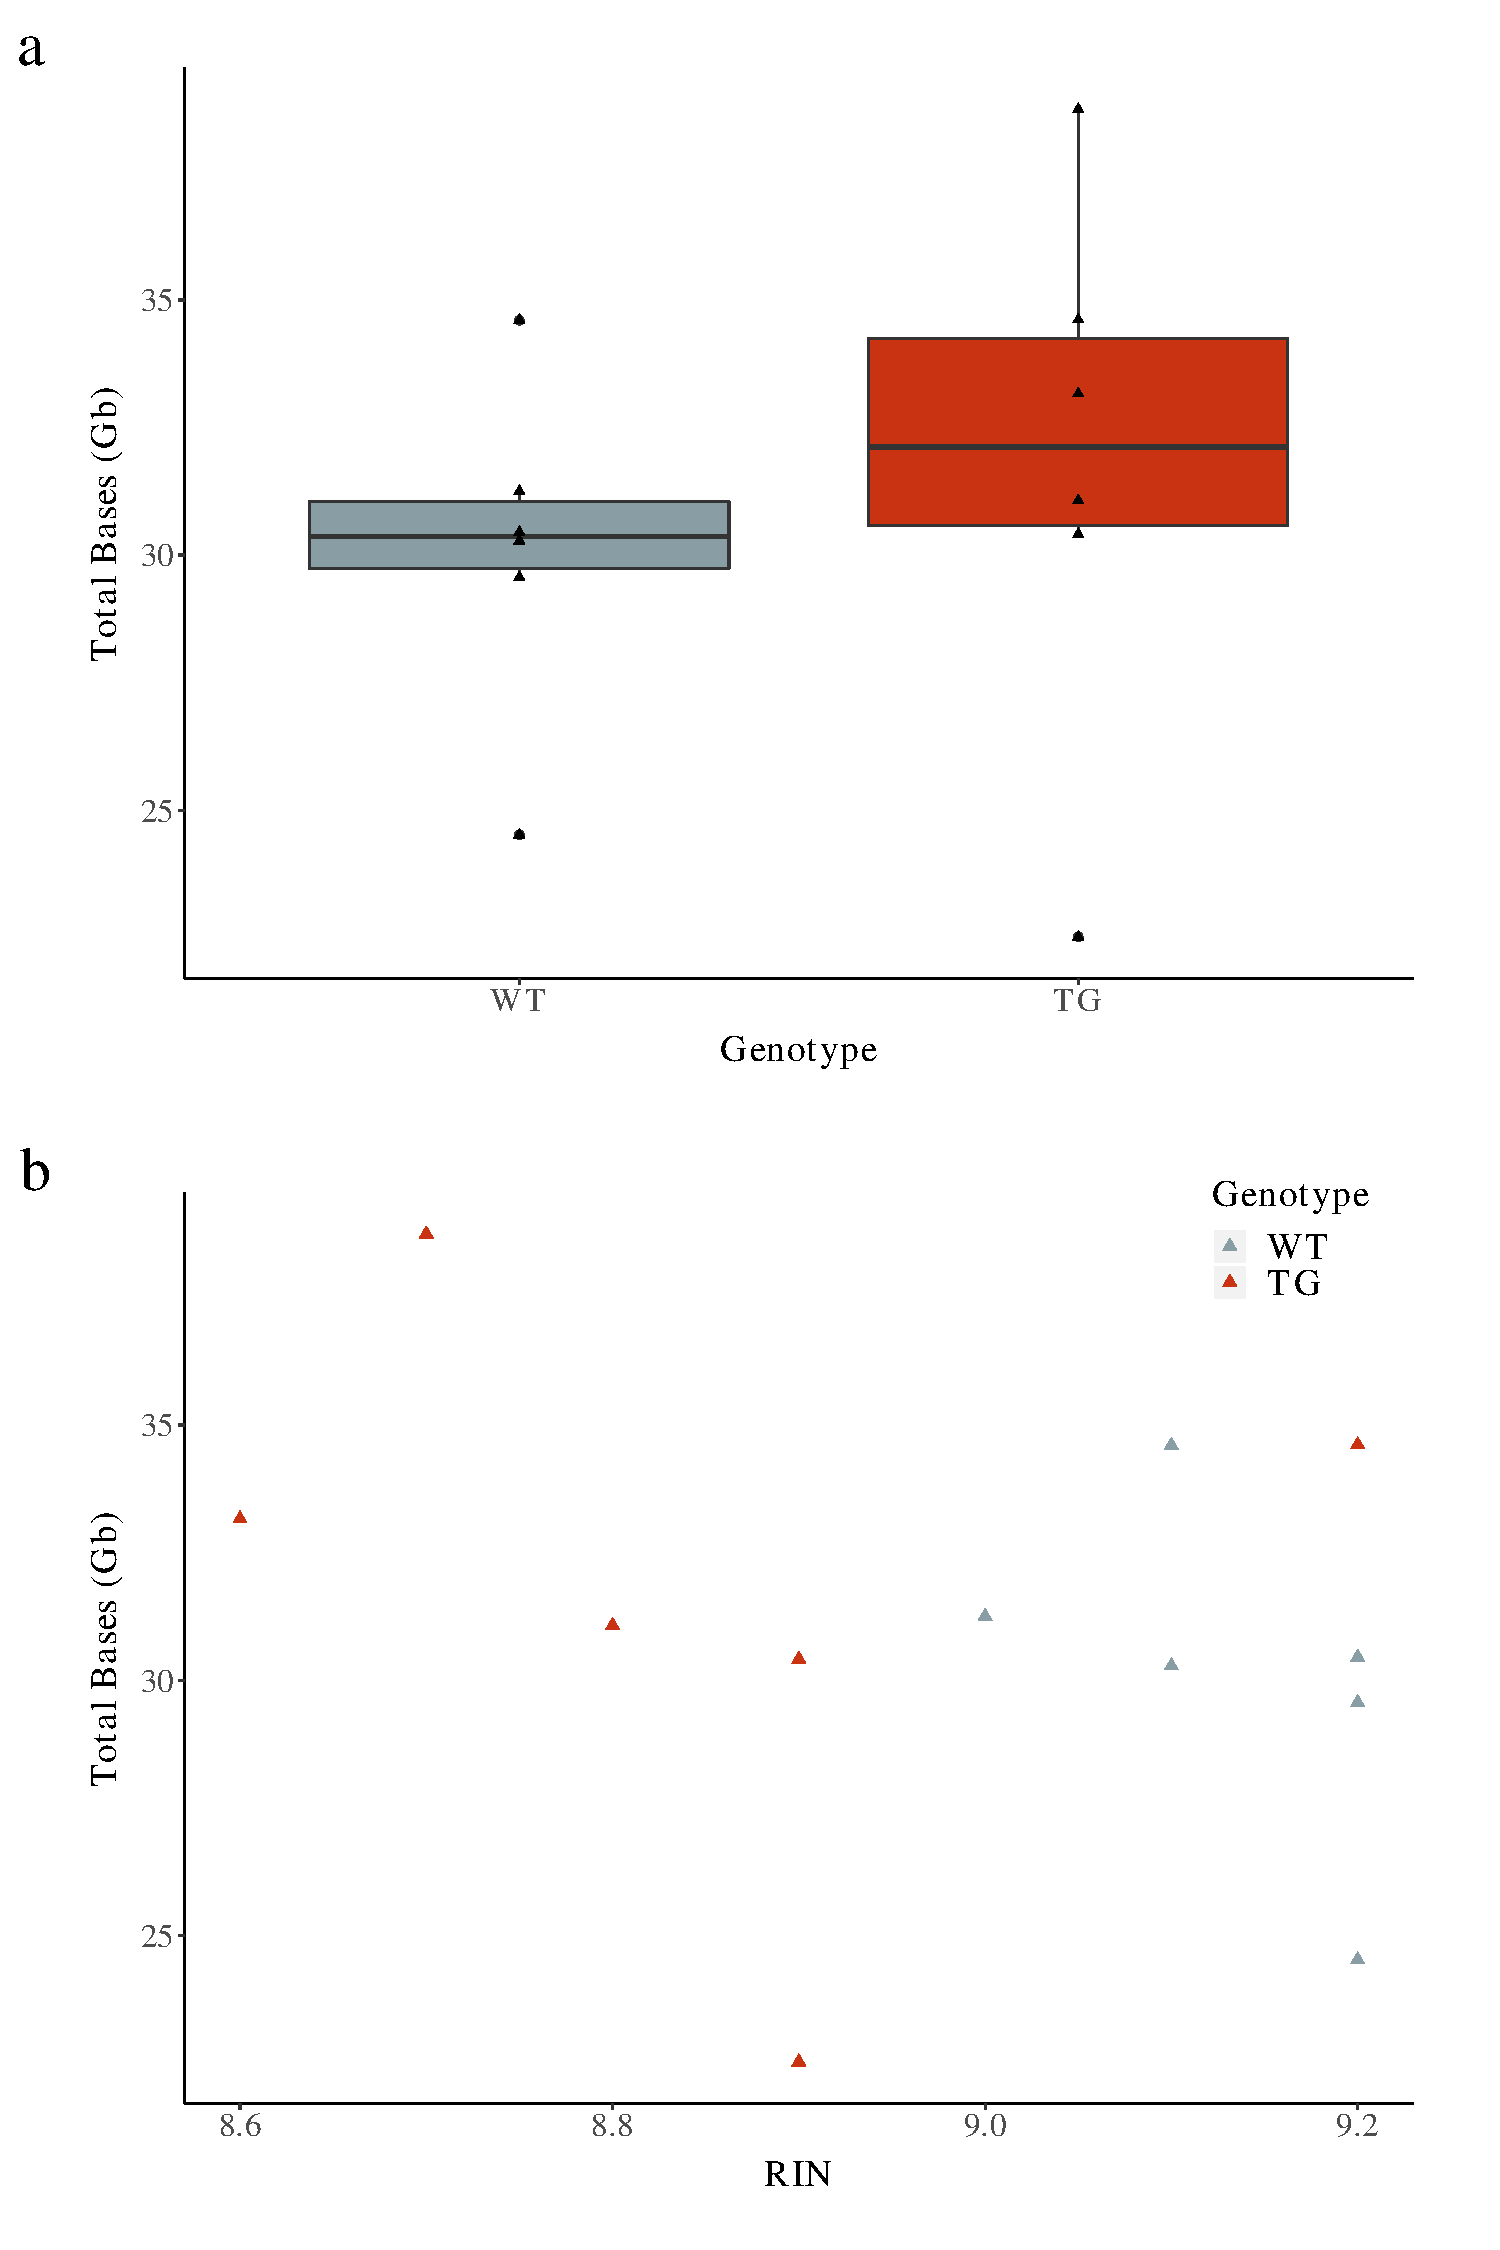
\includegraphics[page=1,trim={0 1cm 0 0},clip,scale = 0.55]{Figures/IsoSeqWholeTranscriptome.pdf}
	\end{center}
	\captionsetup{width=0.95\textwidth}
	\caption[Whole Transcriptome Iso-Seq run yields and relationship to RIN score]%
	{\textbf{Whole Transcriptome Iso-Seq runs generated \textasciitilde30Gb per sample, independent of RIN score}: Sequential Iso-Seq run generated \textbf{a)} a range of 30-35Gb per sample of the whole transcriptome, with no significant difference observed between WT and TG Tg4510 mice. Of note, two samples with $<$25Gb in WT and TG refer to earlier samples sequenced with a lower chemistry. \textbf{b)} Despite TG samples having distinctly lower RIN values than WT samples, no significant difference in yield output was observed between WT and TG.}
	\label{fig:isoseq_whole_run_output}
\end{figure}

\begin{landscape}
	\begin{table}[]
		\resizebox{1.5\textwidth}{!}{%
		\begin{tabular}{@{}cccccccccccccccccc@{}}
			\toprule
			\multirow{3}{*}{Sample} &
			\multirow{3}{*}{\begin{tabular}[c]{@{}c@{}}Polymerase\\ Reads\end{tabular}} &
			\multicolumn{6}{c}{Read   Length} &
			\multicolumn{3}{c}{Productivity} &
			\multicolumn{4}{c}{Control} &
			\multirow{3}{*}{\begin{tabular}[c]{@{}c@{}}Local\\  Base \\ Rate\end{tabular}} &
			\multicolumn{2}{c}{Template} \\ \cmidrule(lr){3-15} \cmidrule(l){17-18} 
			&
			&
			\multicolumn{2}{c|}{Polymerase} &
			\multicolumn{2}{c|}{Subread} &
			\multicolumn{2}{c|}{Insert} &
			\multicolumn{1}{c|}{\multirow{2}{*}{P0}} &
			\multicolumn{1}{c|}{\multirow{2}{*}{P1}} &
			\multicolumn{1}{c|}{\multirow{2}{*}{P2}} &
			\multicolumn{1}{c|}{\multirow{2}{*}{\begin{tabular}[c]{@{}c@{}}Total   \\ Reads\end{tabular}}} &
			\multicolumn{1}{c|}{\multirow{2}{*}{\begin{tabular}[c]{@{}c@{}}Pol RL  \\ Mean\end{tabular}}} &
			\multicolumn{2}{c|}{Concordance} &
			&
			\multicolumn{1}{c|}{\multirow{2}{*}{\begin{tabular}[c]{@{}c@{}}Adapter   \\ Dimer \\ (0-10bp)\end{tabular}}} &
			\multicolumn{1}{c|}{\multirow{2}{*}{\begin{tabular}[c]{@{}c@{}}Short\\  Insert\\  (11- 100bp)\end{tabular}}} \\ \cmidrule(lr){3-8} \cmidrule(lr){14-15}
			&
			&
			\multicolumn{1}{c|}{Mean} &
			\multicolumn{1}{c|}{N50} &
			\multicolumn{1}{c|}{Mean} &
			\multicolumn{1}{c|}{N50} &
			\multicolumn{1}{c|}{Mean} &
			\multicolumn{1}{c|}{N50} &
			\multicolumn{1}{c|}{} &
			\multicolumn{1}{c|}{} &
			\multicolumn{1}{c|}{} &
			\multicolumn{1}{c|}{} &
			\multicolumn{1}{c|}{} &
			\multicolumn{1}{c|}{Mean} &
			\multicolumn{1}{c|}{Mode} &
			&
			\multicolumn{1}{c|}{} &
			\multicolumn{1}{c|}{} \\ \midrule
			B21 &
			735598 &
			39971 &
			82100 &
			1531 &
			2125 &
			3162 &
			3896 &
			\begin{tabular}[c]{@{}c@{}}8.71\% \\ (87817)\end{tabular} &
			\begin{tabular}[c]{@{}c@{}}73.94\% \\ (745646)\end{tabular} &
			\begin{tabular}[c]{@{}c@{}}18.33\% \\ (184883)\end{tabular} &
			9940 &
			34144 &
			0.85 &
			0.89 &
			2.61 &
			0 &
			0 \\
			C20 &
			749931 &
			45670 &
			91153 &
			1426 &
			2066 &
			3204 &
			4075 &
			\begin{tabular}[c]{@{}c@{}}10.68\% \\ (107699)\end{tabular} &
			\begin{tabular}[c]{@{}c@{}}75.36\% \\ (759912)\end{tabular} &
			\begin{tabular}[c]{@{}c@{}}14.95\% \\ (150735)\end{tabular} &
			9910 &
			37019 &
			0.85 &
			0.89 &
			2.75 &
			0 &
			0 \\
			C21 &
			530395 &
			44208 &
			87750 &
			2258 &
			2794 &
			3358 &
			4250 &
			\begin{tabular}[c]{@{}c@{}}38.0\% \\ (387661)\end{tabular} &
			\begin{tabular}[c]{@{}c@{}}52.5\% \\ (535299)\end{tabular} &
			\begin{tabular}[c]{@{}c@{}}9.4\% \\ (96275)\end{tabular} &
			4880 &
			50690 &
			0.85 &
			0.85 &
			2.07 &
			0.00 &
			0.01 \\
			E18 &
			545,272 &
			41,036 &
			83,295 &
			2,467 &
			3,049 &
			3,588 &
			4,335 &
			\begin{tabular}[c]{@{}c@{}}38.88\% \\ (396026)\end{tabular} &
			\begin{tabular}[c]{@{}c@{}}53.61\% \\ (546027)\end{tabular} &
			\begin{tabular}[c]{@{}c@{}}7.58\% \\ (77181)\end{tabular} &
			722 &
			48,253 &
			0.85 &
			0.85 &
			2 &
			0 &
			0 \\
			K17 &
			673972 &
			43856 &
			90561 &
			1253 &
			2021 &
			3336 &
			4753 &
			\begin{tabular}[c]{@{}c@{}}10.55\% \\ (106,736)\end{tabular} &
			\begin{tabular}[c]{@{}c@{}}67.42\% \\ (681,794)\end{tabular} &
			\begin{tabular}[c]{@{}c@{}}22.73\% \\ (229,816)\end{tabular} &
			7036 &
			34651 &
			0.85 &
			0.89 &
			2.72 &
			0.08 &
			0.06 \\
			K18 &
			566086 &
			54892 &
			101220 &
			1256 &
			1775 &
			2863 &
			3661 &
			\begin{tabular}[c]{@{}c@{}}29.77\%\\ (299933)\end{tabular} &
			\begin{tabular}[c]{@{}c@{}}57.25\% \\ (576863)\end{tabular} &
			\begin{tabular}[c]{@{}c@{}}14.05\% \\ (141550)\end{tabular} &
			10707 &
			44640 &
			0.87 &
			0.89 &
			3.05 &
			0 &
			0 \\
			K23 &
			698178 &
			49563 &
			98801 &
			1697 &
			2670 &
			3779 &
			4779 &
			\begin{tabular}[c]{@{}c@{}}16.1\% \\ (164308)\end{tabular} &
			\begin{tabular}[c]{@{}c@{}}69.2\%  \\ (704197)\end{tabular} &
			\begin{tabular}[c]{@{}c@{}}14.7\%   \\ (149841)\end{tabular} &
			5951 &
			40498 &
			0.85 &
			0.89 &
			2.78 &
			0 &
			0 \\
			K24 &
			711015 &
			48675 &
			97024 &
			1714 &
			2487 &
			3834 &
			5018 &
			\begin{tabular}[c]{@{}c@{}}14.22\% \\ (144813)\end{tabular} &
			\begin{tabular}[c]{@{}c@{}}70.49\%\\  (717880)\end{tabular} &
			\begin{tabular}[c]{@{}c@{}}15.28\% \\ (155653)\end{tabular} &
			6762 &
			38363 &
			0.85 &
			0.87 &
			2.671 &
			0.01 &
			0.01 \\
			L22 &
			675283 &
			57370 &
			112630 &
			1869 &
			2867 &
			3903 &
			4793 &
			\begin{tabular}[c]{@{}c@{}}17.41\%\\ (175439 )\end{tabular} &
			\begin{tabular}[c]{@{}c@{}}68.08\%\\ (686007)\end{tabular} &
			\begin{tabular}[c]{@{}c@{}}15.58\% \\ (156900)\end{tabular} &
			10647 &
			44215 &
			0.86 &
			0.89 &
			2.96 &
			0.01 &
			0 \\
			M21 &
			660841 &
			46082 &
			91628 &
			2234 &
			2754 &
			3952 &
			4733 &
			\begin{tabular}[c]{@{}c@{}}16.6\%\\ (168567)\end{tabular} &
			\begin{tabular}[c]{@{}c@{}}65.9\%  \\ (671224)\end{tabular} &
			\begin{tabular}[c]{@{}c@{}}17.5\% \\  (178555)\end{tabular} &
			10301 &
			38690 &
			0.85 &
			0.87 &
			2.79 &
			0.01 &
			0.01 \\
			O18 &
			530974 &
			42423 &
			85331 &
			2609 &
			3146 &
			3443 &
			4082 &
			\begin{tabular}[c]{@{}c@{}}41.8\% \\  (426378\end{tabular} &
			\begin{tabular}[c]{@{}c@{}}52.6\%\\  (536435)\end{tabular} &
			\begin{tabular}[c]{@{}c@{}}5.5\% \\ (56422)\end{tabular} &
			5415 &
			49778 &
			0.86 &
			0.85 &
			2.05 &
			0 &
			0 \\
			O23 &
			730733 &
			42771 &
			89372 &
			1490 &
			2347 &
			3608 &
			4878 &
			\begin{tabular}[c]{@{}c@{}}9.37\% \\ (94536)\end{tabular} &
			\begin{tabular}[c]{@{}c@{}}73.33\% \\ (740184)\end{tabular} &
			\begin{tabular}[c]{@{}c@{}}18.19\% \\ (183626)\end{tabular} &
			8908 &
			34993 &
			0.85 &
			0.89 &
			2.56 &
			0.06 &
			0.04 \\
			Q20 &
			715206 &
			46360 &
			92519 &
			1,999 &
			2,926 &
			3,978 &
			4,954 &
			\begin{tabular}[c]{@{}c@{}}11.51\%\\  (117223)\end{tabular} &
			\begin{tabular}[c]{@{}c@{}}70.91\% \\ (722135)\end{tabular} &
			\begin{tabular}[c]{@{}c@{}}17.58\%\\  (178988)\end{tabular} &
			6855 &
			37990 &
			0.85 &
			0.87 &
			2.6 &
			0.01 &
			0.01 \\
			Q21 &
			733495 &
			33429 &
			70750 &
			2563 &
			3286 &
			3710 &
			4750 &
			\begin{tabular}[c]{@{}c@{}}15.9\% \\ (161679)\end{tabular} &
			\begin{tabular}[c]{@{}c@{}}72.1\%\\  (735250)\end{tabular} &
			\begin{tabular}[c]{@{}c@{}}12.0\% \\ (122305)\end{tabular} &
			1668 &
			44201 &
			0.85 &
			0.85 &
			1.99 &
			0.00 &
			0.01 \\
			S18 &
			682529 &
			44549 &
			90041 &
			1435 &
			2041 &
			3282 &
			4400 &
			\begin{tabular}[c]{@{}c@{}}11.98\%\\  (121,055)\end{tabular} &
			\begin{tabular}[c]{@{}c@{}}68.45\% \\ (691651)\end{tabular} &
			\begin{tabular}[c]{@{}c@{}}20.35\%\\  (205,640)\end{tabular} &
			7881 &
			36541 &
			0.86 &
			0.89 &
			2.85 &
			0.11 &
			0.07 \\
			S23 &
			704335 &
			42991 &
			89160 &
			1346 &
			2020 &
			3272 &
			4383 &
			\begin{tabular}[c]{@{}c@{}}7.02\%\\  (71074)\end{tabular} &
			\begin{tabular}[c]{@{}c@{}}70.18\% \\ (710471)\end{tabular} &
			\begin{tabular}[c]{@{}c@{}}23.39\% \\ (236801)\end{tabular} &
			6019 &
			35167 &
			0.85 &
			0.89 &
			2.57 &
			0.01 &
			0.01 \\ \bottomrule
		\end{tabular}%
	}
	\end{table}
\end{landscape}

With the application of long-reads bioinformatics pipeline (as detailed in Section X), the raw reads were processed and clustered to unique consensus transcripts, which were then mapped and annotated as isoforms - low-quality, lowly-supported, unmapped and degraded reads were sequentially filtered at each stage. Across all 12 samples, a total of 5.66M CCS reads (mean = 471K,s.d = 46.8K, range =  353K - 512K) and 4.55 FLNC reads were successfully generated (mean = 379K, s.d = 47.0K, range = 270K - 412K) after multiple processing (\cref{fig:isoseq_whole_processing}\textbf{a}). Clustering of these reads yielded a total of 273K high-quality full-length transcripts (97\% of all FL transcripts, mean = 32.7K, s.d = 1.25K, range = 30.3K - 34.4K) (\cref{fig:isoseq_whole_processing}\textbf{b}), and were mapped to 278K and 352 loci of the mouse reference (5K had multi-mapping) and ERCC annotations respectively. After filtering for 85\% alignment identity and 95\% length (\cref{fig:isoseq_whole_processing}\textbf{c}), 266K transcripts were retained. 

Showcasing the sensitivity of the sequencing platform and approach, only 62\% (n = 57) of ERCCs were detected, those of which were more highly expressed and with a threshold concentration of XX (\cref{fig:isoseq_whole_ercc}\textbf{a}). However of those ERCCs detected, the number of FL reads detected was highly correlated to the known amount used (corr = 0.98, P = 1.42 x 10\textsuperscript{-41} \cref{fig:isoseq_whole_ercc}\textbf{b}), highlighting the power of Iso-Seq to quantify highly-expressed transcripts. 

\begin{figure}[htp]
	\begin{center}
		\includegraphics[page=11,trim={0 1cm 0 0},clip,scale = 0.55]{Figures/IsoSeqWholeTranscriptome.pdf}
	\end{center}
	\captionsetup{width=0.95\textwidth}
	\caption[Whole Transcriptome Iso-Seq run yields and relationship to RIN score]%
	{\textbf{Whole Transcriptome Iso-Seq runs generated \textasciitilde30Gb per sample, independent of RIN score}: Sequential Iso-Seq run generated \textbf{a)} a range of 30-35Gb per sample of the whole transcriptome, with no significant difference observed between WT and TG Tg4510 mice. Of note, two samples with $<$25Gb in WT and TG refer to earlier samples sequenced with a lower chemistry. \textbf{b)} Despite TG samples having distinctly lower RIN values than WT samples, no significant difference in yield output was observed between WT and TG.}
	\label{fig:isoseq_whole_lengths}
\end{figure}

\begin{figure}[htp]
	\begin{center}
		\includegraphics[page=2,scale = 0.55]{Figures/IsoSeqWholeTranscriptome.pdf}
	\end{center}
	\captionsetup{width=0.95\textwidth}
	\caption[Sequential processing and alignment of reads from Whole Transcriptome Iso-Seq run]%
	{\textbf{Sequential processing of Iso-Seq Reads generated around 32K transcripts per sample with good alignment to reference genome}: \textbf{a)} Processing of Iso-Seq reads generated a similar number of reads across all sample throughout Iso-Seq3 bioinformatis pipeline, with the exception of 2 earlier samples. \textbf{b)} Despite this, all the samples had similar number of FL transcripts with no signficant difference observed between WT and TG. \textbf{c)}The majority of transcipts aligned to mouse reference genome (mm10) with >85\% alignment identity and $>$95\% length}
	\label{fig:isoseq_whole_processing}
\end{figure}

\begin{figure}[htp]
	\begin{center}
		\includegraphics[page=6,trim={0 25cm 0 0},clip,scale = 0.55]{Figures/IsoSeqWholeTranscriptome.pdf}
	\end{center}
	\captionsetup{width=0.95\textwidth}
	\caption[Detection of ERCC standards in Whole Transcriptome Iso-Seq]%
	{\textbf{Over 60\% of ERCCs were detected with highly accurate quantification} \textbf{a} Highly-concentrated ERCCs were detected as single molecules, as expected, and \textbf{b} the number of full-length reads associated for each detected ERCC was highly correlated to known amount. FL - Full Length}
	\label{fig:isoseq_whole_ercc}
\end{figure}


\newpage
\subsection{Nanopore Sequencing run performance and sequencing metrics}
As a technological comparison, two of the samples sequenced on the PacBio Sequel were also sequenced on the ONT MinION. In contrast to the Iso-Seq, the run performance and yield was significantly poorer and lower with greater variability observed between the two samples (K18: 10.1Gb from nanopore vs 31.1Gb from Iso-Seq, M21: 3.68Gb from nanopore vs 30.45Gb from Iso-Seq, \cref{tab:ont_wholerun_output}). The significantly low performance of M21 was due to saturation and permanent blocking of pores (\cref{fig:ont_seq_channel}\textbf{b}) with more rapid decline of sequencing activity than is expected (\cref{fig:ont_time_performance}\textbf{b}). No difference in the sequencing speed was observed across the course of the run (\cref{fig:ont_speedvstime}), however, suggesting that the sequencing chemistry and flow cell was of good quality. The low performance output of the second sample is therefore likely due to introduction of air bubbles and contamination during library preparation.

After removing low-quality basecalled reads (QV < 7), a total of 6M reads were acquired (K18: 4.49M reads, 66\% of total reads, M21: 1.68M reads, 79.2\%, \cref{tab:ont_passedreads_output}). Interestingly, despite the marked lower run performance of the second sample, the read quality was slightly higher (K18: mean QV = 9.5, M21: mean QV = 10.2) whereby the first sample had a large portion of very low-quality reads (QV < 2, \cref{fig:ont_lengthquality}\textbf{a}). Nevertheless, both samples had a very similar read length distribution profile (\cref{fig:ont_lengthquality}\textbf{c,d}), with a mean length around 1.8Kb. However in contrast to Iso-Seq, the distribution is skewed to the left with enrichment of smaller molecules (1kb) - a likely reflection of the library size with no size enrichment during library preparation rather than a length bias of the technology. 

Despite the relatively low run performance, more reads were acquired per flow cell per sample than per SMRT cell in Iso-Seq (mean number of basecalled reads from nanopore across 2 samples: 4.43M, mean number of polymerase reads from Iso-Seq across 12 samples: 0.67M). This is because while Iso-Seq was able to generate very long polymerase reads (mean length across 12 samples = 46kb), contributing to the run yield in gigabases, the number of reads generated per run was limited to 1M (number of SMRT cells). Conversely, there was no upper limit in the number of reads that can be generated with nanopore sequencing provided the pores remained active. A greater proportion of ERCCs (68 ERCCs, 73.9\%) was therefore observed in one nanopore run compared to 12 Iso-Seq runs (57 ERCCs, 62\%), and for those ERCCs detected, the number of FL reads detected was also highly correlated to the known amount used (corr = 0.98, P = 9.73 x 10\textsuperscript{-51}). 


\vspace{1cm}
\begin{table}[ht]
	\centering
	\begin{tabularx}{1\textwidth}{@{}ccccc@{}}
		\toprule
		\multirow{2}{*}{Sample} & \multicolumn{2}{c}{All Reads}      & \multirow{2}{*}{Active channels} & \multirow{2}{*}{Run Duration} \\ \cmidrule(lr){2-3}
		& Total Bases (Gb) & Number of Reads &                                  &                               \\ \midrule
		K18                     & 10.1             & 6,752,951       & 479                              & 48hours                       \\
		M21                     & 3.68             & 2,122,012       & 425                              & 48hours                       \\ \bottomrule
	\end{tabularx}
	\captionsetup{justification=raggedright,width=0.95\textwidth}
\caption[Run Yield Output from Whole Transcriptome Nanopore Sequencing of Tg4510]%
{\textbf{Poorer run performance and lower yield output observed from Nanopore Sequencing of Whole Transcriptome}. Two samples, sequenced on PacBio Sequel using Iso-Seq approach, were also sequenced on ONT MinION on two separate flow cells over 48hours. The number of total reads basecalled was less than a third of the reads generated on the same samples from the Iso-Seq approach (\cref{tab:isoseq_wholerun_output})}
\label{tab:ont_wholerun_output}
\end{table}

\vspace{2cm}
\begin{table}[ht]
	\centering
	\begin{tabularx}{1\textwidth}{@{}ccccccccc@{}}
		\toprule
		\multirow{2}{*}{Sample} & \multirow{2}{*}{\begin{tabular}[c]{@{}c@{}}Total Bases\\ (Gb)\end{tabular}} & \multirow{2}{*}{\begin{tabular}[c]{@{}c@{}}Number of\\  Reads\end{tabular}} & \multicolumn{4}{c}{Read Length (bp)} & \multicolumn{2}{c}{Read Quality} \\ \cmidrule(l){4-9} 
		&                                                                             &                                                                             & Median  & Mean & N50  & Longest Read & Median           & Mean          \\ \midrule
		K18                     & 8.21                                                                        & \begin{tabular}[c]{@{}c@{}}4,468,629 \\ (66.2\%)\end{tabular}               & 1400    & 1838 & 2521 & 48877        & 9.6              & 9.5           \\
		M21                     & 3.1                                                                         & \begin{tabular}[c]{@{}c@{}}1,679,931\\  (79.2\%)\end{tabular}               & 1410    & 1845 & 2644 & 82984        & 10.3             & 10.2          \\ \bottomrule
	\end{tabularx}
	\captionsetup{justification=raggedright,width=0.95\textwidth}
	\caption[ONT Sequencing metrics for pass basecalled reads]%
	{\textbf{Sequencing metrics of filtered high-quality reads}. Basecalled reads were filtered on quality score with a QV threshold of 7. N50 refers to the sequence length at which 50\% of reads are sized at or over. Gb - Gigabases}
	\label{tab:ont_passedreads_output}
\end{table}

\begin{figure}[htp]
	\begin{center}
		\includegraphics[page=1,scale = 0.45]{Figures/ONTWholeTranscriptome.pdf}
	\end{center}
	\captionsetup{width=0.95\textwidth}
	\caption[ONT Sequence Channel Activity from Whole Transcriptome Sequencing ]%
	{\textbf{Sequencing channel activity plot from nanopore sequencing}. Heatmap representation of channel productivity spatially for \textbf{a)} Sample K18 (10.1Gb) and \textbf{b)} Sample M21 (3.68Gb) as DNA is translocated through the pore and signal is collected. A stark contrast of activity can be seen between the two samples, with a significant number of inactive channels (white box) in Sample M21 - of the channels that are active, fewer DNA molecules are translocated and read.  Of note, the activity shows the number of sequences generated per channel not per pore, given that each channel corresponds to four different pores.}
	\label{fig:ont_seq_channel}
\end{figure}

\begin{figure}[htp]
	\begin{center}
		\includegraphics[page=2,,trim={0 0cm 0cm 10cm},clip, scale = 0.45]{Figures/ONTWholeTranscriptome.pdf}
	\end{center}
	\captionsetup{width=0.95\textwidth}
	\caption[ONT run performance over time from Whole Transcriptome Sequencing ]%
	{\textbf{Temporal run performance from nanopore sequencing}. Shown is the \textbf{a)} number of basses generated per hour over the course of the sequencing run from Sample K18 and from \textbf{b)} Sample M21, and \textbf{c)} cumulative reads generated from Sample K18 and from \textbf{d)} Sample M21. The reads are classified as "pass" (dark blue) if QV > 7 and "fail" (light blue) if QV < 7. The rapid decline of pore activity of Sample M21 is evident from Figure b) in contrast to Figure a), with 90\% of the sequencing data acquired within the first 10hours of the run (Figure d). T50 and T90 refers to the time point at which 50\% and 90\% of total basecalled reads where acquired respectively. Gb - Gigabases}
	\label{fig:ont_time_performance}
\end{figure}

\begin{figure}[htp]
	\begin{center}
		\includegraphics[page=4,trim={1cm 0cm 0cm 20cm},clip, scale = 0.45]{Figures/ONTWholeTranscriptome.pdf}
	\end{center}
	\captionsetup{width=0.95\textwidth}
	\caption[ONT translocation speed against time from Whole Transcriptome Sequencing]%
	{\textbf{DNA translocation speed against time}. A boxplot of the translocation speed (sequencing rate) for Sample M21 over the course of the 48-hour run. }
	\label{fig:ont_speedvstime}
\end{figure}

\begin{figure}[htp]
	\begin{center}
		\includegraphics[page=3,trim={0 0cm 0cm 10cm},clip, scale = 0.45]{Figures/ONTWholeTranscriptome.pdf}
	\end{center}
	\captionsetup{width=0.95\textwidth}
	\caption[ONT read length and quality from Whole Transcriptome Sequencing ]%
	{\textbf{Length and quality distribution of ONT basecalled reads}. Shown are histograms of the number of sequenced reads against \textbf{a)} mean read quality score of Sample K18, \textbf{b)} mean read quality score of Sample M21, and against \textbf{c)} length of Sample K18 and of \textbf{d)} Sample M21. The distribution has been shaded for reads that have passed or failed the quality filter (Q-score threshold of 7). N50 refers to the sequence length at which 50\% of reads are sized at or over. }
	\label{fig:ont_lengthquality}
\end{figure}

\begin{figure}[htp]
	\begin{center}
		\includegraphics[page=4,trim={0 16cm 0cm 0},clip, scale = 0.45]{Figures/Pipeline.pdf}
	\end{center}
	\captionsetup{width=0.95\textwidth}
	\caption[ONT read quality against read length from Whole Transcriptome Sequencing ]%
	{\textbf{Distribution of quality scores against read lengths for all ONT basecalled reads}. Shown are 2D density plots for \textbf{a)} Sample K18 and \textbf{b)} Sample M21 of mean sequence quality (Phred quality score) against read length (log10). Figures are generated from PycoQC \cite{Leger2019}.}
	\label{fig:ont_lengthvsquality}
\end{figure}

\clearpage
\subsection{Transcriptome annotation}
After further collapsing and filtering of transcripts using the Iso-Seq data, a total of 46,626 unique and intact isoforms were identified (mean = 27.5K, s.d = 2.32K, range = 24.2K - 31.2K) and annotated to 14,482 (98.6\%) known and 202 (1.38\%) novel genes. Gene expression patterns from Iso-Seq reflected expected transcriptional profiles for the brain regions profiled. Using the Mouse Gene Atlas database, the 500 most abundantly-expressed genes were most significantly enriched for ‘cerebral cortex’ (odds ratio = 6.07, adjusted P = 6.8 x 10\textsuperscript{-17}). Rarefaction curves confirmed that the dataset approached saturation, indicating that our coverage of isoform diversity was representative of the true population of transcripts (\cref{fig:isoseq_whole_rarefaction}\textbf{a}). Supporting the validity of these isoforms, the majority (n = 35,262, 75\% of isoforms) were enriched near an annotated CAGE peaks (located within 50bp), and the vast majority of unique splice junctions (n = 138,032, 97.8\% of junctions) were supported by RNA-Seq.

\begin{figure}[htp]
	\begin{center}
		\includegraphics[page=3,scale = 0.55]{Figures/IsoSeqWholeTranscriptome.pdf}
	\end{center}
	\captionsetup{width=0.95\textwidth}
	\caption[Rarefaction Curves of Whole Transcriptome Iso-Seq Runs]%
	{\textbf{Rarefaction curve of Iso-Seq merged dataset indicated saturation and good coverage of genes and isoforms}:}
	\label{fig:isoseq_whole_rarefaction}
\end{figure}

\newpage
\subsection{Isoform diversity}
Compared with the mouse reference genome, there was a wider range in the number of isoforms identified per gene (1 – 86), with each gene associated with a median of 2 isoforms. Only 10\% (n = 4,641) of isoforms were detected across all the samples (\cref{fig:isoseq_whole_lowlyexp}\textbf{a}), with about half (47.8\%) detected in 2 - 3 samples with very low transcript expression (\cref{fig:isoseq_whole_lowlyexp}\textbf{b}).

Gene ontology (GO) analysis showed that the most enriched molecular function amongst the 100 most transcriptionally diverse genes in mouse cortex was ‘tubulin binding’ (odds ratio = 7.90, adjusted P =  6.70 x 10\textsuperscript{-4}), driven by the overexpression of MAPT in TG mice.
%an interesting observation given the role that RNA-binding proteins (RBPs) themselves play in regulating tissue-specific patterns of alternative splicing. 
%Any differences between samples not due to absence or presence of isoform but isoform proportion/ not deep enough?   
   
A significant proportion of isoforms (20,621, 45\%) were sized 2 - 4kb in length (median length = 2.96kb, mean length = 3.18kb, s.d = 1.68kb, range = 0.083 - 15.9kb) (\cref{fig:isoseq_whole_isoform_length_corr}\textbf{a}), corresponding to the mean length of mRNA mouse reference genome, with a wide range in the number of exons (1 - 89) observed per isoform (mean number of exons = 10.8). The number of isoforms per gene was correlated with gene length (corr = 0.25, P = 1.33 x 10 \textsuperscript{-197}, \cref{fig:isoseq_whole_isoform_length_corr}{c}), and exon number (corr = 0.24, P = 7.97 x 10 \textsuperscript{-155}, \cref{fig:isoseq_whole_isoform_length_corr}{d}). 

\begin{figure}[htp]
	\begin{center}
		\includegraphics[page=4,trim={0 25cm 0 0},clip,scale = 0.55]{Figures/IsoSeqWholeTranscriptome.pdf}
	\end{center}
	\captionsetup{width=0.95\textwidth}
	\caption[Isoform diversity across Tg4510 samples and coverage of ERCC transcripts]%
	{\textbf{Highly-expressed isoforms are more likely to be sequenced across sampples and accurately quantified}: Shown is \textbf{a)} the distribution of isoforms detected in the number of mouse samples, with a third detected in any two of the total 12 samples. However, \textbf{b)} quantification of these isoforms had very low expression (1-2 FL read), whereas those that were commonly detected across all 12 samples were very highly expressed. FL - Full Length}
	\label{fig:isoseq_whole_lowlyexp}
\end{figure}

\begin{figure}[htp]
	\begin{center}
		\includegraphics[page=5,trim={0 12cm 0 0},clip,scale = 0.55]{Figures/IsoSeqWholeTranscriptome.pdf}
	\end{center}
	\captionsetup{width=0.95\textwidth}
	\caption[Correlation of isoform diversity with transcript length and number of exons]%
	{\textbf{Longer genes with more exons were associated with more isoforms}: \textbf{a} The majority of isoforms have a length between 1 - 5kb. \textbf{b)} The number of exons was correlated with the transcript length, and the \textbf{c)} the number of isoforms was correlated with the length and \textbf{d)} and the number of exons per gene. Gene length and exon number is represented by the longest transcript. kb - kilobases}
	\label{fig:isoseq_whole_isoform_length_corr}
\end{figure}


\newpage
\subsection{Iso-Seq vs RNA-Seq} 
To compare the power of Iso-Seq versus RNA-Seq to detect full-length transcripts, a reference-guided transcriptome assembly using only Illumina's RNA-Seq reads of the same samples was generated with Stringtie. Using SQANTI to characterise isoforms similarly to the Iso-Seq analysis, RNA-Seq defined transcriptome revealed significantly more isoforms (156,253 isoforms vs 46,626 isoforms from Iso-Seq defined transcriptome, \cref{fig:isoseq_whole_rnaseqvsisoseq}\textbf{a}). However, upon further examination and comparison using gffcompare, majority of these isoforms were found to be incomplete fragments of isoforms identified in Iso-Seq, with significantly shorter isoform length (2.31kb vs 3.18kb of mean length of RNA-Seq and Iso-Seq defined isoforms respectively, two-tailed unpaired t-test, t(203070) = 71.9, P < 2.2 x 10\textsuperscript{-16}, \cref{fig:isoseq_whole_rnaseqvsisoseq}\textbf{c}), fewer exons (7.30 vs 10.8 of mean number of exons of RNA-Seq and Iso-Seq defined isoforms respectively, two-tailed unpaired t-test, t(203070) = 76.7, P < 2.2 x 10\textsuperscript{-16}, \cref{fig:isoseq_whole_rnaseqvsisoseq}\textbf{d}) and less supported by CAGE peaks (34.0\% vs 71.9\% of RNA-Seq and Iso-Seq defined isoforms within 50bp CAGE peak respectively, Fisher's Test: P < 2.2 x 10\textsuperscript{-16}, odds ratio = 4.97, \cref{fig:isoseq_whole_rnaseqvsisoseq}\textbf{e}). Considering only isoforms that had a complete exact match as defined by gffcompare, more than 50\% of isoforms detected from Iso-Seq dataset could not be readily recapitulated (\cref{fig:isoseq_whole_rnaseqvsisoseq}\textbf{a}), the majority of which were novel isoforms and genes (\cref{fig:isoseq_whole_rnaseqvsisoseq}f).      

The isoform expression (TPM) was then compared using the following methods: 
\begin{enumerate}
	\item Iso-Seq data alone using FL read count 
	\item RNA-Seq data aligned to Iso-Seq defined transcriptome using Kallisto\cite{Bray2016}
	\item RNA-Seq data aligned to RNA-Seq defined transcriptome using Kallisto\cite{Bray2016}. RNA-Seq transcriptome was generated using Stringtie. 	
\end{enumerate}

Focusing only on the subset of isoforms that were commonly identified in both RNA-Seq and Iso-Seq defined transcriptomes (n = 23,761), the isoform expression using RNA-Seq data mapped to Iso-Seq (method 2) and RNA-Seq transcriptome (method 3) was highly correlated (Pearson's correlation = 0.77, P < 2.2 x 10\textsuperscript{-16}). Conversely, the isoform expression derived from Iso-Seq data alone (method 1) was weekly correlated to the RNA-Seq derived isoform expression (method 3, Pearson's correlation = 0.45, P < 2.2 x 10\textsuperscript{-16}). This highlights the power of Iso-Seq defined transcriptome to accurately identify and annotate isoforms as a scaffold, but is limited for quantitative analysis due to sequencing depth.

\begin{figure}[htp]
	\begin{center}
		\includegraphics[page=13,scale = 0.55]{Figures/IsoSeqWholeTranscriptome.pdf}
	\end{center}
	\captionsetup{width=0.95\textwidth}
	\caption[RNA-Seq defined transcriptome]%
	{\textbf{Iso-Seq identified more isoforms per gene, that were longer with more exons, and with a greater proportion of isoforms with CAGE peak}: A reference-guided transcriptome using only RNA-Seq data (RNA-Seq defined transcriptome) was generated. \textbf{a)} RNA-Seq defined transcriptome identified more isoforms, as expected given the significantly higher sequencing depth. However, \textbf{b)} the isoform diversity was smaller than that from Iso-Seq defined transcriptome with the majority of genes associated with only one isoform. \textbf{c)} Isoforms identified from the RNA-Seq defined transcriptome were also more likely to be shorter and \textbf{d} contain fewer exons. \textbf{e)} Highlighting the power of Iso-Seq to identify true full-length isoforms in comparison to RNA-Seq, a significantly larger proportion of isoforms from Iso-Seq data were found within 50bp of a CAGE peak. \textbf{f} Approximately half of the isoforms identified using Iso-Seq were novel (NIC, NNC), which were not recapitulated using RNA-Seq. FSM - Full Splice Match, ISM - Incomplete Splice Match, NIC - Novel In Catalogue, NNC - Novel Not in Catalogue.}   
	\label{fig:isoseq_whole_rnaseqvsisoseq}
\end{figure}


\subsection{Novel isoforms}
\label{sec:whole_novelIso}
Interestingly, the transcriptome was made up of 50\% of isoforms that were known (23,350) and 50\% that were novel (23,096) and were not present in existing annotation databases (\cref{tab:sqanti_output_whole}). Benchmarking the accuracy and reliability of novel isoforms against known isoforms, no difference in the number supported within 50bp CAGE was observed (novel isoforms within CAGE: 17,252, 75.4\%; known isoforms with CAGE: 17,842, 75.8\%, Fisher's Test: P = 0.31, odds ratio = 0.978). Less RNA-Seq support was observed for novel isoforms compared to known isoforms (mean RNA-Seq expression for known isoforms = 8.95TPM, mean RNA-Seq expression for novel isoforms = 1.99TPM; two-tailed unpaired t-test: t(46401) = 14.8, P = 1.37 x 10\textsuperscript{-49}); however, this is likely to reflect RNA-Seq's lack of power to detect novel isoforms rather than the validity of these isoforms. 

\begin{table}[]
	\begin{tabularx}{1\textwidth}{lcl}
	\toprule
	Description              & \multicolumn{1}{l}{Number} & Isoform Definition               \\ \midrule
	Number of Genes    & 14684                      &                                  \\
	Number of Isoforms & 46626                      &                                  \\
	Annotated Genes          & 14482 (98.62\%)            &                                  \\
	\hspace{3mm}Annotated Isoforms       & 23530 (50.47\%)            &                                  \\
	\hspace{6mm}FSM          & 19803 (42.47\%) & exact alignment as reference  \\
	\hspace{6mm}ISM  & 3727 (7.99\%)   & exact alignment as reference but fewer 5’ exons       \\
	\hspace{3mm}Novel Isoforms           & 23096 (49.53\%)            &                                  \\
	\hspace{6mm}NIC      & 13763 (29.52\%) & a combination of known donor/acceptor sites                    \\
	\hspace{6mm}NNC   & 8751 (18.77\%)  & at least one novel donor/acceptor site    \\
	\hspace{6mm}Fusion                   & 297 (0.64\%)               &                                  \\
	\hspace{6mm}Genic Genomic            & 62 (0.13\%)                & overlaps with introns and exons  \\
	Novel Genes              & 202 (1.38\%)               &                                  \\
	\hspace{6mm}Intergenic               & 104 (0.22\%)               & located in the intergenic region \\
	\hspace{6mm}Antisense                     & 119 (0.26\%)    & opposite-strand orientation to known gene           \\ \bottomrule
	\end{tabularx}
	\caption[Gene and Isoform classification from Whole Transcriptome Iso-Seq of Tg4510]%
	{Classification of annotated and novel genes and isoforms were based from SQANTI2, and from the merging of 12 samples. FSM - Full Splice Match, ISM - Incomplete Splice Match, NIC - Novel In Catalogue, NNC - Novel Not in Catalogue }
	\label{tab:sqanti_output_whole}
\end{table}

Compared to known isoforms, these novel isoforms were less abundant (Mann-Whitney-Wilcoxon test, W = 3.66 x 108, P < 2.23 x 10\textsuperscript{-308} \cref{fig:isoseq_whole_novel_known_iso_corr}\textbf{a,b}) and longer (Mann-Whitney-Wilcoxon test, W = 2.37 x10\textsuperscript{8}, P = 2.13 x 10\textsuperscript{-42}, \cref{fig:isoseq_whole_novel_known_iso_corr}\textbf{c,d}) with more exons (Mann-Whitney-Wilcoxon test, W = 1.94 x 10\textsuperscript{8}, P < 2.23 x 10\textsuperscript{-308}, \cref{fig:isoseq_whole_novel_known_iso_corr}\textbf{e,f}), suggesting that they would have been harder to detect using traditional short-read RNA-Seq due to the difficulty in assembling transcripts with limited read coverage. These novel isoforms were also more likely to be associated with novel transcription start sites (1,454 novel isoforms vs 1,154 annotated isoforms at least 1kb away from known TSS, Fisher's Test: P = 6.16 x 10\textsuperscript{-12}, odds ratio = 1.32) and termination sites (21,506 novel isoforms vs 21,434 annotated isoforms less than 1kb away from known TTS) than known isoforms. 
%lncRNA with RNASeq

\begin{figure}[htp]
	\begin{center}
		\includegraphics[page=7,scale = 0.55]{Figures/IsoSeqWholeTranscriptome.pdf}
	\end{center}
	\captionsetup{width=0.95\textwidth}
	\caption[Comparison of Known and Novel Isoforms from Iso-Seq Whole Transcriptome runs]%
	{\textbf{Novel isoforms were less expressed, longer and had more exons than known isoforms}: Shown is the \textbf{a)} Iso-Seq transcript expression, the \textbf{c)} transcript length, and the \textbf{e)} the number of exons of novel and known isoforms. The known and novel isoforms can be further subdivided and classified, with the \textbf{b)} Iso-Seq expression \textbf{d)} transcript length and \textbf{f)} number of exons for each category. According to SQANTI, known isoforms are subdivided into FSM and ISM, and novel isoforms are subdivided into NIC, NNC, and fusion. FSM – Full Splice Match, ISM – Incomplete Splice Match, NIC – Novel In Catalogue, NNC – Novel Not in Catalogue.}   
	\label{fig:isoseq_whole_novel_known_iso_corr}
\end{figure}


The different types of splicing events were also compared between known and novel isoforms (see Section X). In total, 40,249 alternative splicing events were identified in annotated genes with AF (alternative TSS variation) and SE being the most prevalent events (AF: 12,853, 31.9\%; SE: 8,686, 21.6\%, \cref{fig:isoseq_whole_As_events}). It is important to note, however, that only around 30\% of 5'end isoforms were located near (<5bp) any annotated 5' end whereas 70\% of 3' ends were located near (<5bp) annotated 3'ends - this discrepancy is likely due to a combination of mRNA degradation, template switching artifacts during reverse transcription and true novel alternative TSS. 

Except for AF and AL, all the other different splicing events, and in particularly intron retention, were more likely to be observed in novel isoforms than in known isoforms, implicating the power of Iso-Seq to detect full-length transcripts and the ability to recapitulate the usage of complex splicing events that would have otherwise been underestimated with only RNA-Seq data alone (Fisher's one-tailed Test, A3: P = 7.78 x 10 \textsuperscript{–14}, odds ratio = 1.34; A5: P = 1.21 x 10\textsuperscript{–13}, odds ratio = 1.45, IR: P < 2.23 x 10\textsuperscript{–16}, odds ratio = 4.92; MX: P = 4.18 x 10\textsuperscript{–11}, odds ratio = 1.81; SE: P < 2.23 x 10\textsuperscript{–16}, odds ratio = 1.57, \cref{fig:isoseq_whole_As_events}). 

\begin{figure}[htp]
	\begin{center}
		\includegraphics[page=8,trim={0 19cm 0 2cm},clip,scale = 0.55]{Figures/IsoSeqWholeTranscriptome.pdf}
	\end{center}
	\captionsetup{width=0.95\textwidth}
	\caption[Number of Alternative Splicing Events in Whole Transcriptome Iso-Seq]%
	{\textbf{Alternative first is the most prevalent AS event, and novel isoforms are more likely to be characterised with complex AS events}: Shown is the proportion of AS events in annotated genes, and further subdivided by known and novel isoforms. Novel isoforms were more likely to be characterised by all AS events, with the exception of AF and AL. MX and SE events were determined using SUPPA2, IR with SQANTI2 and A3’, A5’, AF and AL with custom scripts. AF – Alternative First Exon, AL – Alternative Last Exon, A5’ – Alternative 5’ prime, A3’ – Alternative 3’ prime, IR – Intron Retention, MX – Mutually Exclusive, SE – Skipped Exon}
	\label{fig:isoseq_whole_As_events}
\end{figure}

\subsection{Intron Retention and Nonsense mediated decay}
For the majority of genes characterised by splicing, only one or two splicing events were observed (n = 10,708, 81.8\% of AS genes, \cref{tab:AS_events_spliced}), suggesting that such events were often mutually independent. However, interestingly, Nonsense-mediated mRNA decay (NMD) - a mechanism that acts to reduce transcriptional errors by degrading transcripts containing premature stop codon - was found to be particularly enriched amongst isoforms characterised with intron retention (IR-isoforms\nomenclature{IR-isoforms}{Intron-retained isoforms}). Of the 6,803 isoforms characterised with intron retention, 38.7\% (n = 1,930) were also predicted to undergo NMD (NMD-isoforms\nomenclature{NMD-isoforms}{Isoforms characterised with nonsense mediated decay}), as characterised by the presence of an ORF and a coding sequence (CDS) end motif before the last junction. Novel isoforms, more likely to be characterised with intron retention, were also more likely to be associated with NMD than known isoforms (Fisher's Test: P < 2.23 x 10\textsuperscript{-16}, odds ratio = 4.16). 

These isoforms with both IR and NMD were found to more lowly expressed than isoform only with NMD and no IR (W = 7.50 x 10\textsuperscript{6}, P = 1.67 x 10\textsuperscript{-42}, \cref{fig:isoseq_whole_IRNMD}\textbf{b}), those of which were also more lowly expressed than isoforms with no NMD. Furthermore, only a small number of genes were associated with isoforms where IR and NMD were mutually exclusive (n = 277, 1.91\% of total genes, \cref{fig:isoseq_whole_IRNMD}\textbf{a}), providing additional support for the hypothesized relationship between these two transcriptional control mechanisms.

\begin{table}[ht]
	\centering
	\begin{tabularx}{0.6\textwidth}{cc}
		\toprule
		Number of Splicing Events & Frequency \\ \midrule
		1                           & 7315 (55.89\%)                \\
		2                           & 3393 (25.92\%)                \\
		3                           & 1724 (13.17\%)                \\
		4                           & 548 (4.19\%)                  \\
		5                           & 108 (0.83\%)                  \\ \bottomrule
	\end{tabularx}
	\caption[Number of Splicing Events]%
	{Shown is the number of splicing events observed in genes that are alternatively spliced. Majority of genes are detected with only one or two splicing events.}
	\label{tab:AS_events_spliced}
\end{table}


\begin{figure}[htp]
	\begin{center}
		\includegraphics[page=9,trim={0 1cm 0 0.5cm},clip,scale = 0.55]{Figures/IsoSeqWholeTranscriptome.pdf}
	\end{center}
	\captionsetup{width=0.95\textwidth}
	\caption[Association of intron retention and NMD in Whole Transcriptome Iso-Seq]%
	{\textbf{Intron retention is associated with nonsense-mediated mRNA decay (NMD) and reduced expression}: Shown is the overlap of genes associated with isoforms characterised with intron retention (IR), nonsense-mediated mRNA decay (NMD), and transcripts with both IR and NMD (IR-NMD). Of note, genes with isoforms characterised by both IR and NMD were further classified into genes that contain isoforms where both events are observed together (purple) and where they are mutually exclusive (dark orange). As such, 13800 genes were associated with IR-isoforms that were predicted for NMD, and 168 genes that contained IR-isoforms and NMD-isoforms. Isoforms that were characterised with both IR and NMD were particularly lowly expressed compared to isoforms with either IR, NMD or neither events. IR – Intron Retention, NMD – Nonsense-mediated mRNA decay.}
	\label{fig:isoseq_whole_IRNMD}
\end{figure}

\subsection{Fusion Genes}
Transcriptional read-through between two (or more) adjacent genes can produce ‘fusion transcripts’ that represent an important class of mutation in several types of cancer32. Although fusion events are thought to be rare, we found that ~0.4\% of transcripts included exons from two or more adjacent genes (mouse cortex: n = 297 fusion transcripts associated with 218 genes (1.51\%)). 


\subsection{LncRNA}
Although the majority of isoforms (93.6\%, 43,450) mapping to known genes were classified as protein-coding by the presence of an ORF, a relatively large number of isoforms (n = 1,141) were mapped to genes annotated as encoding lncRNA (n = 734 genes). Compared to isoforms not defined as lncRNA (non-lncRNA) by reference genome, these lncRNA isoforms were found to be longer (Mann-Whitney-Wilcoxon test, W = 3.52 x 10\textsuperscript{7}, P = 8.24 x 10\textsuperscript{-98}, \cref{fig:isoseq_whole_lncRNA}\textbf{a}), despite containing fewer exons (W = 4.56 x 10\textsuperscript{7}, P < 2.23 x 10\textsuperscript{-308}, \cref{fig:isoseq_whole_lncRNA}\textbf{b}) and being enriched for mono-exonic molecules(23.9\% vs 2.02\%) - corroborating previous findings from other long-read studies(\cite{Derrien2012},\cite{Tilgner2015}). These lncRNA isoforms were found to be more lowly expressed than non-lncRNA isoforms (W = 3.16 x 10\textsuperscript{7}, P = 5.67 x 10\textsuperscript{-40}), with fewer RNA isoforms identified per lncRNA gene (mean n = 1.55, range = 1 - 34 vs mean n = 3.29, range = 1 - 86; W = 7.40 x 10\textsuperscript{6}, P = 5.76 x 10\textsuperscript{-107}, \cref{fig:isoseq_whole_lncRNA}\textbf{e}). 

Importantly, over a third (448, 39.3\%) of these annotated lncRNA isoforms contained a putative ORF, supporting recent observations that lncRNA have potential protein coding capacity, with shorter ORFs than non-lncRNA isoforms (mean length = 139bp, s.d = 127bp vs mean length = 519bp, s.d = 393bp; W = 1.75 x 10\textsuperscript{7}, P = 8.33 x 10\textsuperscript{-195}). 

\begin{figure}[htp]
	\begin{center}
		\includegraphics[page=10,scale = 0.55]{Figures/IsoSeqWholeTranscriptome.pdf}
	\end{center}
	\captionsetup{width=0.95\textwidth}
	\caption[Characterisation of LncRNA in Whole Transcriptome runs]%
	{\textbf{LncRNA isoforms were more lowly expressed and typically longer than non-lncRNA transcripts, despite containing fewer exons}: Shown is the distribution of the \textbf{a)} transcript length, \textbf{b)} number of exons, \textbf{c)} transcript expression, \textbf{d)} ORF length and the \textbf{e)} diversity of isoforms annotated to lncRNA and non-lncRNA.lncRNA – long non-coding RNA}
	\label{fig:isoseq_whole_lncRNA}
\end{figure}

\subsection{Novel Genes}
\label{sec:whole_novelgenes}
Although the vast majority of isoforms were annotated to known genes, 0.5\% (n = 223 isoforms) did not and potentially represent "novel" genes (n = 189 genes). These novel genes were all multi-exonic (mean length = 1.75kb, s.d = 1.21kb, range = 0.098 - 6.86kb, mean number of exons = 2.5) and were identified uniformly across the genome/chromosome, with over half the identified transcripts from these genes predicted to be non-coding (n = 143 (64.1\%) novel-gene transcripts), shorter and more lowly expressed than annotated genes (length: W = 7.79 x 10\textsuperscript{6}, P = 5.22 x 10\textsuperscript{-45}; expression: W = 2.29x 10\textsuperscript{6}, P = 1.5 x 10\textsuperscript{-73}).

%https://www.ncbi.nlm.nih.gov/pmc/articles/PMC6885035/ - Lorna’s paper on example of isoforms in their selective panel of genes that have differential quantification associated with AD. Good examples to check with transcriptome data to see if this is also observed in mouse (I.e. TAU3 increase) 

\newpage
\section{Discussion}
"The apparent length limitation to 6kb is most likely a combined result of ineffective size selection and the limitation ofthe sequencing chemistry (P4-C2, Methods) used in this study"; what are the proportion of transcripts relative to genome in size? The length of clustered transcripts closely reflect size distribution of the input full-length reads. "Final transcripts include a large number of isoforms greater than 3 kb that are not accessible by simply using CCS reads."   

Although skipped exons are known to be the most common AS events in mouse, our data conversely suggests that splice variants from a single gene are predominantly generated through alternative first exons 
%Single cell analysis (\cite{Karlsson2017}) noted that alternative TSS and TTS variation in the first exon representing more than 70\% of splicing events,

\chapter{Transcriptional differences between WT and TG mice}\label{ch: transcriptional_global_differences}
%Classification of AS events, which most commonly observed/dominant? Isoforms derived from transcriptional regulation (alternative promoters) vs post-transcriptional regulation? 
%Impact of AS events on protein domains. Non-sense mediated decay? 
%%Furthermore changes in gene/transcript expression can be due to differences in cellular composition (i.e. neuronal loss/reactive gliosis) rather than indicative of disease-associated transcriptional regulation. 
%%Gene expression and mRNA isoforms vary widely across tissues (\cite{Wang2008}), thus sequencing the disease-relevant tissue (in this case entorhinal cortex) is important for understanding the pathology of AD. However, it is consequently important to note that other tissues may have to be considered to fully grasp the whole picture of AD development. 

\section{Introduction}

Following the accurate characterisation of the mouse transcriptome using long-read sequencing from a global (whole transcriptome approach, \cref{ch: whole_transcriptome}), this chapter aims to exploit these datasets to investigate the transcriptional changes in the mouse entorhinal cortex associated with tau pathology. 

There have been multiple studies recently that explore the transcriptional differences in transgenic mice harbouring different mutations associated with AD. However, all of these studies to date have been undertaken with short-read RNA-Seq - which, while it offers obvious advantage compared to microarrays in accurately quantifying gene expression, is severely limited in detecting and characterising transcripts (as discussed in detail in \cref{rnaseq_intro}). Given that short-reads fail to span the entire length of transcripts, characterising and quantifiying alternatively-spliced isoforms is inferred computationally after alignment by using statistical models, which is computationally challenging - a survey of current tools revealed only 40\% of known human transcripts were assembled \cite{Steijger2013}.  

While there have been significant advances to process long-read sequencing data for transcriptome annotations, methods to harness long-read data for downstream statistical analyses have been limited. These analyses include identifying genes or transcripts with a significant change in expression across biological conditions (the process of which is referred to as Differential Gene Expression, DEG, and Differential Transcript Expression, DTE, analysis respectively), and are typically analysed using statistial tools such as \textit{DESeq}, \textit{edgeR}, \textit{limma}, among others. However, these tools were developed in response to the emergence of short-read RNA-Seq analysis, and typically involve i) aligning short-reads to transcripts either from de-novo assembly or using a reference annotation, and then ii) estimating the transcript expression using complex algorithms. Various benchmarking studies have been conducted to compare the performance of such tools \cite{Teng2016,Rapaport2013}, concluding that there was no single favourable method although tools based on negative binomial modelling (\textit{DESeq}, \textit{edgeR})) had better specificity, sensitivity and good control of false positive errors\cite{Rapaport2013}. 


Currently, all the new tools developed to process long-read sequencing data (such as Oxford Nanopore's recommended cDNA transcriptome tutorial \cite{ONTcdna_transcriptome}, \textit{FLAIR} \cite{Tang2020}) integrate old tools, which were initially designed to analyse short-read sequencing data, for differential gene and isoform analyses. Systematically assessed and benchmarked for detecting differential splicing and expression at isoform level in RNA-Seq studies, \textit{DESeq2}, \textit{DexSeq} and \textit{NOISeq} have been most widely used. 
 
%Genome-wide RNAseq study of the molecular mechanisms underlying microglia activation in response to pathological tau perturbation in the rTg4510 tau transgenic animal model - PubMed (nih.gov)
%Integrating human brain proteomes with genome-wide association data implicates new proteins in Alzheimer's disease pathogenesis - PubMed (nih.gov)
%The role of microglia in processing and spreading of bioactive tau seeds in Alzheimer’s disease | Journal of Neuroinflammation | Full Text (biomedcentral.com) 
%%https://actaneurocomms.biomedcentral.com/articles/10.1186/s40478-018-0574-5 - rTg4510

\section{Methods}

\subsection{Iso-Seq Processing and Isoform Quantification}
All analyses pertaining to this chapter follows on from \cref{wholetranscriptome} and \cref{targetedmousetranscriptome}: raw Iso-Seq reads from the individual samples were processed using \textit{IsoSeq3}, which were them merged to one complete transcriptome at the global and targeted level, before transcript collapse with \textit{Cupcake}, alignment with \textit{Minimap2}, annotation with \textit{SQANTI3} (v3.3) and finally, additional filtering with \textit{TAMA}. Of note, transcriptome was reannotated with \textit{SQANTI3} due to \text{SQANTI2} being no longer maintained and the addition of novel features in \textit{SQANTI3}, including the generation of a functionally-labelled annotation from the long-reads. 

The full-length long-read counts (abundance) for each sample, required for downstream analyses, were obtained from one of \textit{cupcake's} output files (read\_stat.txt), which documented the source of all the full-length transcripts that were used for isoform collapse. Given that samples were sequenced individually under the whole transcriptome approach, we were thus able to differentiate and count the transcripts using the Run ID. For the targeted transcriptome approach, whereby the samples were barcoded and thus could not be differentiated by sequencing run, we used the ID (original CCS read) documented in the output file (flnc.report.csv) from \textit{Iso-Seq3 Refine} after sample demultiplexing. 


\subsection{Quantification of human MAPT transgene expression} 
As a quality check of sample identity, the presence of human- and mouse-specific Mapt/MAPT sequences was determined in full-length transcripts across all the samples. Species-specific MAPT sequence, located in a 2kb region present in the 3'UTR, was identified after using BLAT\cite{Kent2002} to compare human and mouse MAPT/Mapt sequence for divergent transcript sequences \cite{Castanho2020}).  

\subsection{Characterisation of Alternative Splicing Events} 
Alternative splicing events were examined using a range of packages and custom scripts, as described and implemented in \label{sec:AS_methods}, to assess whether there was a change in splicing patterns associated with rTg4510 pathology and across age. 


\subsection{Differential expression analysis}
After trialling various ad-hoc methods, I chose to explore the transcriptomic changes between wildtype and transgenic mice with \textit{tappAS} (v1.0.0)\cite{DeLaFuente2020}, which was also developed by the same authors as \textit{SQANTI} (A.Conesa's group) and was recommended as an extension to the Iso-Seq pipeline for the functional annotations of isoforms. Accessible as a user-friendly Java application, \textit{tappAS} was chosen as the framework for differential expression analysis due to the flexibility to explore both genotype effects and progressive changes across age, and to optimise parameters as background scripts were fully accessible and clearly written.

\textit{tappAS} requires three inputs\cite{DeLaFuente2020}:
\begin{enumerate}
	\item An experimental design file, which allows comparisons to be made between two or more groups and/or over a time-course 
	\item A transcript-level functional annotation file, which is generated post \textit{SQANTI} using \textit{IsoAnnot} (another tool developed by A.Conesa's group, https://isoannot.tappas.org), as a "scaffold" for transcript-level annotations. For the purpose of this study, the annotation file would be the conglomerate, long-read defined transcriptome of all the samples merged. 
	\item A transcript level expression matrix, which can either be derived directly from the full-length long-read transcript counts, or from mapping and transcript quantification of short-reads to the long-read defined transcriptome using \textit{Kallisto}(v0.46.0). Raw transcript counts were tabulated per sample.  	 
\end{enumerate}

As a method comparison, the expression from both short- and long-read was used as quantification at the gene and transcript level, such that four differential analyses were performed using the whole and targeted transcriptome datasets (\cref{tab:dea_analyses_summary}). To explore the utility and power of long reads for transcriptome annotation, results from the differential gene analyses were also compared to that generated from I.Castanho's analyses \cite{Castanho2020}. 
%brief statement of isabel's analyses  

\begin{table}[h]
	\centering
	\begin{tabularx}{0.9\textwidth}{cccc}
		\toprule
		& Datasets                                         & Annotation                                                                                                          & Quantification   \\ \midrule
		1 & \multirow{2}{*}{Whole Transcriptome  (n = 12)}   & \multirow{4}{*}{\begin{tabular}[c]{@{}c@{}}Iso-Seq reads \\ processed using\\ bioinformatics pipeline\end{tabular}} & Iso-Seq FL reads \\
		2 &                                                  &                                                                                                                     & RNA-Seq reads    \\
		3 & \multirow{2}{*}{Targeted Transcriptome (n = 24)} &                                                                                                                     & Iso-Seq FL reads \\
		4 &                                                  &                                                                                                                     & RNA-Seq reads    \\ \bottomrule
	\end{tabularx}
	\caption[Differential Gene and Transcript Analyses for mouse transcriptome using whole and targeted Iso-Seq transcriptome datasets]%
	{Summary of the differential gene and transcript analyses for mouse transcriptome using whole and targeted Iso-Seq transcriptome datasets. Using the Iso-Seq defined transcriptome as the "scaffold" rather than mouse reference genome, the analyses primarily differed on the quantification input. FL - Full length.}
	\label{tab:dea_analyses_summary}
\end{table}

\boldheader{Count Normalisation}
% Discussion of expression 
%The choice to use quantification directly from long-reads or derived indirectly from short-reads is dependent on the read coverage. While there will be no assembly ambiguity in using the abundance counts from long-reads, the coverage from the whole transcriptome approach would be insufficient for meaningful quantitative analyses - as shown in the coverage with ERCC (see Figure \cref{fig:isoseq_whole_ercc}) with lowly-expressed transcripts not being detected. Conversely, this is unlikely to be a limiting factor for the targeted transcriptome approach given the saturation coverage of target genes with additional sequencing of off-target, highly-expressed genes (see Figure \cref{fig:isoseq_targeted_rate}). Consequently, the expression matrix input for the whole transcriptome analyses was derived from the short-read alignment, and from the long-read abundance for the targeted transcriptome analyses. 
Very lowly-expressed transcripts with a sum of expression value less than 1 CPM (counts per million\nomenclature{CPM}{Counts per million}) or a large variance (>100 Coefficient of Variation) across all the samples were removed to reduce noise. The raw transcript counts were then normalised using TMM normalisation \cite{Robinson2010} (Trimmed Mean of M-values\nomenclature{TMM}{Trimmed Mean of M-values}) to account for differences in library size (sequencing depth) and sample RNA library composition, which is particularly important when comparing samples from different genotypes. The difference in RNA composition is determined by calculating a "scaling factor" for each sample relative to a reference sample (sample with the least varying read counts), which is the weighted average of all the log2 ratio of transcript counts between the two samples (M-values). The weighted average does not consider log2 ratio of transcripts with significant differences ("biased" transcripts that are widely present in one sample and not the other, and vice versa) and of transcripts with highest or lowest expression, hence "trimmed mean", to avoid effect of outliers. Of note, TMM assumes that the majority of the transcripts are not differentially expressed. Gene abundance was deduced from the sum of normalised counts of associated isoforms, after removing transcripts with low or highly-varied expression values.     

\boldheader{Differential Gene and Isoform Expression Analysis}
To elucidate transcriptional changes for both genotype and longitudinal effects between two groups and over time, \textit{maSigPro} \cite{Conesa2006,Nueda2014,Conesa2017} was used for both differential gene and transcript expression analysis, implemented as part of \textit{tappAS}. Briefly, maSigPro performs a two-step regression strategy to first define a negative binomial general linearised models\cite{Nueda2014} for each gene or transcript, accounting for both genotype and age (Equation \cref{eq:dea_lm_masigpro}), and identify differentially expressed genes. A stepwise regression is then applied to identify the conditions for which the differentially expressed genes have statistically significant profiles.  

Adapting the model\cite{Conesa2006} to our scenario, let \textit{I} denote the genotype groups (wildtype - WT, transgenic - TG) and \textit{J} as the age (2, 4, 6, 8 months) for each particular group, and assuming that gene or transcript expression in measured in replicated samples (\textit{R}).  

\begin{myequation}[!h]
\begin{align}\label{eq:dea_lm_masigpro}
y_{ijr} =  \:&\beta_{0} + \beta_{1}D_{ijr} \nonumber
\\ &+ \delta_{0}T_{ijr} + \delta_{1}T_{ijr}D_{ijr}   \nonumber
\\ &+ \gamma_{0}T_{1ijr}^{2} + \gamma_{1}T_{ijr}^{2}D_{ijr} \nonumber
\\ &+ \lambda _{0}T_{ijr}^{3} + \lambda_{1}T_{ijr}^{3}D_{ijr} + \varepsilon_{ijr} \nonumber
\end{align}
where:
\begin{conditions*}
	y_{ijr} & normalised expression value for each gene or transcript in the situation \textit{ijr} (genotype group \textit{i} at age \textit{j} of replicate \textit{r}) \\
	D  &  dummy binary variable to distinguish between the genotype groups, whereby 0 refers to reference group (WT) and 1 refers to experimental group (TG) \\
	T  &  age at 2, 4, 6, 8 months described using a polynomial model with a degree of 3 \\
	\beta_{0}, \delta_{0}, \gamma_{0}, \lambda _{0} & regression coefficients for reference group (WT) relating to the age \\ 
	\beta_{1}, \delta_{1}, \gamma_{1}, \lambda _{1} & regression coefficients for the difference between the experimental group (TG) and reference group (WT) at each age  
\end{conditions*}
therefore, if:
\begin{conditions*}
	FDR(\beta_{1}) < 0.05 & significant expression difference between WT and TG at 2 months \\ 
	FDR(\delta_{0}) < 0.05 & significant expression difference in WT across 2 and 4 months \\
	FDR(\delta_{1}) < 0.05 & significant expression difference between WT and TG across 2 and 4 months \\
\end{conditions*}
\hspace*{10mm}...
\captionsetup{width=0.95\textwidth}
\caption[Linear regression model to determine differential gene and transcript expression]%
{\textbf{Linear regression model to determine differential gene and transcript expression}. The model, adapted from \textit{MaSigPro} and implemented as part of \textit{tappAS}, describes gene or transcript expression between two groups (WT - wildtype, TG - transgenic) at four different time points (age in months). FDR - False discovery rate}    
\end{myequation}

\begin{figure}[!htp]
	\centering
	\includegraphics[page=2,trim={0 5cm 0 4cm},scale = 0.45]{Figures/WholeDifferentialAnalysis.pdf}
	\captionsetup{width=0.95\textwidth}
	\caption[Different conditions modelled for exploring rTg4510 genotype across age]%
	{\textbf{Different conditions modelled for exploring rTg4510 genotype across age.} An example of six different models generated with \textit{maSigPro} using Equation \cref{eq:dea_lm_masigpro} for 2 experimental groups (WT - Wildtype/Control, TG - Transgenic/Case) across two time points/age (T1, T2). The regression coefficients from Equation \cref{eq:dea_lm_masigpro} - $\beta_{1}$, $\delta_{0}$, $\delta_{1}$ - refer to the different variables modelled, the significance of which can be used to infer whether there is a genotype, age or interaction effect. The significance is symbolised by the tick and cross, which refers to adjusted P-value (FDR) < 0.05 and > 0.05 respectively. A significance of  $\beta_{1}$ denotes to a statistically significant difference between WT and TG at T1 (Genotype effect),$\delta_{0}$ to a difference in WT over time (Age effect), and $\delta_{1}$ to a difference between WT and TG across age (Interaction effect). \\\\
	\textit{maSigPro} labels the coefficients in the results table as "CaseVsControl", "Time", "TimexCase" for $\beta_{1}$, $\delta_{0}$, $\delta_{1}$. In the case where there is more time points/ages (as experimented in the Targeted Transcriptome datasets), the significance for the additional regression coefficients relating to the additional time variables are reported (Time2, Time2xCase, Time3, Time3xCase)}   
	\label{fig:dea_model}
\end{figure}

A gene or transcript with different profiles between WT and TG mice would have a different corresponding regression model with a statistically significant coefficient (\cref{fig:dea_model}), and was considered differentially expressed if P-value adjusted for multiple testing, by controlling the false discovery rate (FDR\nomenclature{FDR}{False Discovery Rate}) with the Benjamin and Hochberg correction, was < 0.05 and R\textsuperscript{2} > 0.5. The R\textsuperscript{2} defines the proportion of deviance that was explained by the linear regression model ("goodness of fit"), whereby a recommended threshold of 0.5 was used to identify differentially expressed genes with meaningful biological implications \cite{Conesa2006}.

Following the identification of statistically significant gene models (\cref{fig:dea_model}), the specific conditions (phenotype or age-associated changes) for which the genes show statistically significant profile changes (the significant variables) were identified by using an iterative backward stepwise approach \cite{Conesa2017}. The procedure therefore first started with all the variables imputed (different phenotype x age at different time points). At each iteration step, the P-value associated to each variable was determined and only the variables with a P-value < 0.05 were retained. 

\boldheader{Differential Isoform Usage}
\label{ch:diu_method}
In addition to assessing expression changes across conditions through differential isoform expression analysis, the relative expression, and as such the usage, of these isoforms can also change (see \cref{intro:dtu}). A gene is therefore identified as exhibiting differential isoform usage (DIU) if the fraction of the associated isoforms (Isoform Fraction) is significantly altered between conditions, which could result in detection of a different dominant isoform. This phenomenon is known as major isoform switching, when the same isoform in predominantly expressed in one condition (major isoform) but lowly expressed in another (minor isoform). 

In accounting for biological replicates, the isoform fraction (IF) for each isoform was defined as:

\begin{myequation}[!h]
	\begin{align}
	IF_{cig} = \frac{\bar{E}_{cig}}{\sum_{i=1}^{n}\bar{E}_{cig}}
	\end{align}
	where:
	\begin{conditions*}
		\hspace{3mm}\conj{E}\textsubscript{cig} & mean normalised expression for isoform \textit{i} associated to gene \textit{g} under condition \textit{c}\\
		\hspace{3mm}n  & total number of isoforms associated with gene \textit{g}
	\end{conditions*}
	\captionsetup{width=0.95\textwidth}
	\caption[Calculation of isoform fraction for differential isoform usage analysis]%
	{\textbf{Calculation of isoform fraction for differential isoform usage analysis}. Equation is adopted from \textit{tappAS}}    
\end{myequation}

% Need more information from paper on how DIU was performed
Identification of genes with DIU was performed with \textit{Iso-maSigPro}\cite{Nueda2018}, similarly implemented as part of \textit{tappAS}. Results from differential gene expression and differential isoform usage can be further combined to explore the transcriptomic changes associated with progressive tau pathology (depicted in \cref{fig:DIU_DEA_model}).  

Despite abundant evidence of widespread isoform diversity \cite{Wang2008}, most protein-coding genes have been reported to typically express a few dominant isoforms \cite{Gonzalez-Porta2013, Ezkurdia2015}, while the remaining are very lowly expressed and unlikely to be main contributors to the proteome \cite{Gonzalez-Porta2013}.As such, minor isoforms were filtered to avoid finding genes associated with differential isoform usage due to "flat" behaviour of these minor isoforms \cite{DeLaFuente2020} (relatively small non-negligible expression changes of minor isoforms in the opposing direction of the predominant isoforms). \textit{tappAS} provides two strategies to filter lowly-expressed isoforms: an isoform is only retained if its proportion relative to other isoforms is greater than the pre-specified threshold (default: proportion $>$ 10\%) in at least one sample, or alternatively if its proportion relative to the major isoform is below a pre-specified threshold (default: FC = 2). A major isoform is defined as the isoform with the highest expression across all the conditions, with the remaining isoforms annotated as minor. 

Implemented as an additional filtering step after \textit{tappAS} and recommended in other bioinformatic tools\cite{Vitting-Seerup2017}, lowly expressed genes were also filtered as there would be less confidence in isoform fraction used for determining genes with significant differential isoform usage.  

\begin{figure}[htp]
	\begin{center}
		\includegraphics[page=3,trim={1cm 17cm 0cm 0cm},clip,scale = 0.45]{Figures/WholeDifferentialAnalysis.pdf}
	\end{center}
	\captionsetup{width=0.95\textwidth}
	\caption[Scenarios modelled with differential gene expression analysis and isoform usage]%
	{\textbf{Scenarios modelled with differential gene expression analysis and isoform usage.} A schematic figure to outline the different scenarios modelled under differential gene expression and differential isoform usage analysis. A gene can be differentially expressed between two conditions with differential isoform usage with or without switching of major isoform (Conditions 1 and 2 respectively). Conversely, a gene may not be differentially expressed, due to averaging of isoform expression, but is characterised with differential isoform usage between the two conditions (Conditions 3 and 4)}   
	\label{fig:DIU_DEA_model}
\end{figure}

\clearpage 
\section{Results}

\subsection{Change in endogeneous expression}
%Check whether overexpression of human MAPT result in any unwanted, compensatory effects on equivalent mouse genes,as expression levels of mouse APP and MAPT should be slightly reduced, thereby suggesting no evidence that human transgene expression increase expression of directly-related mouse genes.
As expected, human-specific \textit{MAPT} sequences were only detected in reads from TG mice, confirming stable activation of human \textit{MAPT} transgene (\cref{fig:isoseq_humanmapt}\textbf{a}) and supporting findings from Castanho et al.\cite{Castanho2020}. Alignment of these human-specific transcripts to the mouse genome were mapped either to the mouse prion protein gene (\textit{Prnp}) with high identity but short overlap (\cref{fig:isoseq_humanmapt}\textbf{b,c}), given that the transgene contains exons 2-3 of mouse \textit{Prnp}\cite{Ramsden2005}, and to the mouse \textit{Mapt} gene with low identity but long overlap (\cref{fig:isoseq_humanmapt}\textbf{b,d}). Applying filter thresholds for downstream analysis removed these human-specific \textit{MAPT} transcripts (\cref{fig:isoseq_humanmapt}\textbf{b}). 

\begin{figure}[htp]
	\begin{center}
		\includegraphics[page=1,trim={1cm 20cm 0cm 0cm},clip,scale = 0.55]{Figures/AltFigures_Diff.pdf}
	\end{center}
	\captionsetup{width=0.95\textwidth}
	\caption[Quantifying human-specific and mouse-specific \textit{MAPT}/\textit{Mapt} sequences in Iso-Seq Whole Transcriptome]%
	{\textbf{Human-specific \textit{MAPT} sequences only present in transgenic mice with poor alignment to mouse \textit{Prnp} and \textit{Mapt} gene}: Presence of human- and mouse-specific \textit{MAPT}/\textit{Mapt} sequences was determined in full-length transcripts generated from Iso-Seq merged dataset. \textbf{a)} Ratio of full-length transcripts that were mapped to human-specific \textit{MAPT} and mouse-specific \textit{Mapt} sequences. Dotted lines represent the mean paths across ages. \textbf{b)} As expected, human-specific \textit{MAPT} transcripts were poorly aligned to mouse genome. Transcripts were either aligned to mouse \textit{Prnp} gene (boxed yellow) or  mouse \textit{Mapt} gene (boxed blue). Alignment to mouse \textit{Prnp} gene was near 100\% within a short region, given that the transgene contains exon 2 and 3 of mouse \textit{Prnp} gene\cite{Ramsden2005}. Conversely, while human-specific \textit{MAPT} gene was sufficiently divergent from mouse \textit{Mapt} gene for transgene quantification, it still mapped to the mouse \textit{Mapt} gene 3'UTR albeit poorly. \textbf{c)} USCS genome browser tracks of human-specific (black) \textit{MAPT} transcripts (transgene) and mouse \textit{Prnp} gene and \textbf{d)} mouse \textit{Mapt} gene. Blue tracks represent known transcripts from reference mouse genome (mm10). Tracks were cropped and modified to remove irrelevant genes within the same locus.  UTR - Untranslated region}
	\label{fig:isoseq_humanmapt}
\end{figure}


\subsection{Transcriptome Annotation}
%No difference was observed in the number of transcripts generated between WT and TG (n = 12, two-tailed unpaired t-test, t = -0.005, df = 10, P = 0.996) or by age (n = 12, t = -1.58, df = 10, P = 0.15).
While identifying widespread RNA isoform diversity amongst genes expressed in the mouse entorhinal cortex (described in \cref{wholetranscriptome}), no difference was observed in the number of genes (mean number = 13,302 genes) or isoforms (mean number = 35,157 isoforms) detected between wildtype and trangenic mouse at the two ages (WT: n = 6, TG: n = 6). Further characterisation of the transcriptome revealed similar profile of isoform diversity between the two phenotypes and ages (\cref{tab:isoseq_whole_subsqantioutput}), with half of the isoforms annotated as known (mean number = 18,567 isoforms (52.8\%), as also shown in \cref{sec:whole_novelIso}) and with a similar distribution in isoform length and number of exons (median: 9, range = 1-89) 

\begin{landscape}
	\begin{table}[]
		\centering
		\captionsetup{width=0.95\linewidth}
		\resizebox{1.5\textwidth}{!}{%
	\begin{tabular}{@{}ccccccc@{}}
		\toprule
		& \begin{tabular}[c]{@{}c@{}}Wildtype \\ (n = 6)\end{tabular}              & \begin{tabular}[c]{@{}c@{}}Transgenic\\  (n = 6)\end{tabular}            & \begin{tabular}[c]{@{}c@{}}Wildtype, 2 months \\ (n = 3)\end{tabular}    & \begin{tabular}[c]{@{}c@{}}Wildtype, 8 months\\  (n = 3)\end{tabular}   & \begin{tabular}[c]{@{}c@{}}Transgenic, 2 months \\ (n = 3)\end{tabular}  & \begin{tabular}[c]{@{}c@{}}Transgenic, 8 months \\ (n = 3)\end{tabular}  \\ \midrule
		Total Number of Genes               & 14083                                                                    & 14183                                                                    & 12798                                                                    & 12947                                                                   & 12384                                                                    & 13418                                                                    \\
		Annotated Genes                     & 13911 (98.78\%)                                                          & 14018 (98.84\%)                                                          & 12696 (99.2\%)                                                           & 12816 (98.99\%)                                                         & 12286 (99.21\%)                                                          & 13289 (99.04\%)                                                          \\
		Novel Genes                         & 172 (1.22\%)                                                             & 165 (1.16\%)                                                             & 102 (0.8\%)                                                              & 131 (1.01\%)                                                            & 98 (0.79\%)                                                              & 129 (0.96\%)                                                             \\
		Total Number of Isoforms            & 41081                                                                    & 41671                                                                    & 31407                                                                    & 32630                                                                   & 28982                                                                    & 35169                                                                    \\
		FSM                                 & 18287 (44.51\%)                                                          & 18574 (44.57\%)                                                          & 15503 (49.36\%)                                                          & 15870 (48.64\%)                                                         & 14675 (50.63\%)                                                          & 16892 (48.03\%)                                                          \\
		ISM                                 & 3164 (7.7\%)                                                             & 3242 (7.78\%)                                                            & 2243 (7.14\%)                                                            & 2368 (7.26\%)                                                           & 2066 (7.13\%)                                                            & 2590 (7.36\%)                                                            \\
		NIC                                 & 11781 (28.68\%)                                                          & 12033 (28.88\%)                                                          & 8356 (26.61\%)                                                           & 8856 (27.14\%)                                                          & 7518 (25.94\%)                                                           & 9805 (27.88\%)                                                           \\
		NNC                                 & 7354 (17.9\%)                                                            & 7343 (17.62\%)                                                           & 4980 (15.86\%)                                                           & 5175 (15.86\%)                                                          & 4427 (15.27\%)                                                           & 5520 (15.7\%)                                                            \\
		Genic Genomic                       & 55 (0.13\%)                                                              & 54 (0.13\%)                                                              & 37 (0.12\%)                                                              & 41 (0.13\%)                                                             & 28 (0.1\%)                                                               & 43 (0.12\%)                                                              \\
		Antisense                           & 93 (0.23\%)                                                              & 100 (0.24\%)                                                             & 49 (0.16\%)                                                              & 74 (0.23\%)                                                             & 65 (0.22\%)                                                              & 74 (0.21\%)                                                              \\
		Fusion                              & 253 (0.62\%)                                                             & 242 (0.58\%)                                                             & 180 (0.57\%)                                                             & 176 (0.54\%)                                                            & 155 (0.53\%)                                                             & 177 (0.5\%)                                                              \\
		Intergenic                          & 94 (0.23\%)                                                              & 83 (0.2\%)                                                               & 59 (0.19\%)                                                              & 70 (0.21\%)                                                             & 48 (0.17\%)                                                              & 68 (0.19\%)                                                              \\
		Genic Intron                        & 0 (0\%)                                                                  & 0 (0\%)                                                                  & 0 (0\%)                                                                  & 0 (0\%)                                                                 & 0 (0\%)                                                                  & 0 (0\%)                                                                  \\
		Isoform Length (bp)                 & \begin{tabular}[c]{@{}c@{}}Median: 2946, \\ Range: 83-15016\end{tabular} & \begin{tabular}[c]{@{}c@{}}Median: 2955, \\ Range: 83-15913\end{tabular} & \begin{tabular}[c]{@{}c@{}}Median: 2987, \\ Range: 88-15016\end{tabular} & \begin{tabular}[c]{@{}c@{}}Median: 2890,\\ Range: 83-14850\end{tabular} & \begin{tabular}[c]{@{}c@{}}Median: 2798, \\ Range: 88-14302\end{tabular} & \begin{tabular}[c]{@{}c@{}}Median: 3013, \\ Range: 83-15913\end{tabular} \\
		Number of Exons                     & \begin{tabular}[c]{@{}c@{}}Median: 9, \\ Range: 1-89\end{tabular}        & \begin{tabular}[c]{@{}c@{}}Median: 9, \\ Range: 1-89\end{tabular}        & \begin{tabular}[c]{@{}c@{}}Median: 9, \\ Range: 1-89\end{tabular}        & \begin{tabular}[c]{@{}c@{}}Median: 9, \\ Range: 1-89\end{tabular}       & \begin{tabular}[c]{@{}c@{}}Median: 9, \\ Range: 1-77\end{tabular}        & \begin{tabular}[c]{@{}c@{}}Median: 9, \\ Range: 1-89\end{tabular}        \\
		Number of Isoforms within 50bp CAGE & 34574 (84.16\%)                                                          & 35097 (84.22\%)                                                          & 26539 (84.5\%)                                                           & 27689 (84.86\%)                                                         & 24398 (84.18\%)                                                          & 29911 (85.05\%)                                                          \\ \bottomrule
			\end{tabular}%
		}
	\caption[Overview of the whole transcriptome Iso-Seq datasets generated from mouse rTg4510, subsected by phenotype and age]%
	{Overview of the whole transcriptome Iso-Seq datasets generated from mouse rTg4510, subsected by phenotype and age. Annotations from wildtype (n = 6) and transgenic mouse (n = 6) were generated from merging Iso-Seq datasets from mouse aged 2 and 8 months of the respective phenotype. Novel genes refer to genes that were not currently present in existing genome annotations (mm10). Isoform can be further classified as known (FSM, ISM) or novel (ISM, NIC, NNC, Genic Genomic, Antisense, Fusion, Intergenic, Genic Intron), as described in \cref{sec:sq_exp}. FSM – Full Splice Match, ISM – Incomplete Splice Match, NIC – Novel In Catalogue, NNC – Novel Not in Catalogue.}
	\label{tab:isoseq_whole_subsqantioutput}
		\end{table}
\end{landscape}

\subsection{Alternative Splicing and Functional Diversity}
Transcriptome profiling of the mouse cortex previously identified widespread isoform diversity, driven predominantly by the usage of alternative first exons (AF) and exon skipping (ES) (described in \cref{sec:whole_novelIso}). Upon further examination, there was no significant difference in splicing patterns associated with rTg510 pathology or across age with AF (mean n = 20,400, 40.2\%) as the most prevalent event across all datasets \cref{AS_WholeTranscriptome_diff}. 
%stats?
%XX of known transcripts were identified to have intron retention; XX of known transcripts were identified to be fusion genes. XX of know transcripts identified to have non-sense-mediated decay. 

\vspace{0.5cm}
\begin{table}[!htp]
	\centering
	\captionsetup{width=1\textwidth}
	\caption[Alternative Splicing Events associatd with tau pathology and age]%
	{\textbf{Alternative Splicing Events associatd with tau pathology and age}. Tabulated is the number of splicing events detected for wildtype and transgenic Tg4510 mice aged 2 and 8 months (n = 12, 3 biological replicates per group)}
	\begin{tabular}{@{}ccccc@{}}
		\toprule
		\multirow{2}{*}{Splicing Events} & \multicolumn{2}{c}{Wildtype} & \multicolumn{2}{c}{Transgenic} \\ \cmidrule(l){2-5} 
		& 2 months        & 8 months        & 2 months        & 8 months        \\ \midrule
		A3 & 3394 (6.8\%)    & 3526 (6.82\%)   & 2969 (6.41\%)   & 3825 (6.93\%)   \\
		A5 & 1388 (2.78\%)   & 1456 (2.82\%)   & 1231 (2.66\%)   & 1568 (2.84\%)   \\
		AF & 20185 (40.44\%) & 20597 (39.87\%) & 19182 (41.41\%) & 21781 (39.44\%) \\
		AL & 15620 (31.3\%)  & 16079 (31.12\%) & 14796 (31.94\%) & 16932 (30.66\%) \\
		IR & 3669 (7.35\%)   & 4169 (8.07\%)   & 3017 (6.51\%)   & 4794 (8.68\%)   \\
		MX & 324 (0.65\%)    & 315 (0.61\%)    & 285 (0.62\%)    & 378 (0.68\%)    \\
		SE & 5329 (10.68\%)  & 5524 (10.69\%)  & 4847 (10.46\%)  & 5953 (10.78\%)  \\ \bottomrule
	\end{tabular}
	\label{AS_WholeTranscriptome_diff}
\end{table}

However, aside from changes in splicing patterns, variations in strutural and feature elements annotated across RNA and protein isoforms of the same gene can also have functional implications \cite{DeLaFuente2020}. Using \textit{TappAS}\cite{DeLaFuente2020}, we qualitiatively catalogued the functional diversity of all multi-isoform genes, performing pairwise comparisons between isoforms of the same gene to test for either the i) presence or absence of the annotated feature or ii) in the annotated genomic positions (a feature is classified as varying if the feature's coordinates differ by >9bp between isoforms of the same gene). Of note, many of the protein-defined features can be explored using both approaches given that these elements can be affected through complete skipping (resulting in absence) or partial disruption (resulting in varied genomic position).

Under these two approaches, we identifed that the majority of genes had elements that varied either by absence/presence or by position (\cref{fig:FDA_whole}\textbf{a}). Among elements at a transcript level, miRNA binding had the highest rate of varying (n = 4209 genes) with a large number of miRNA sites varying at the 3'UTR (n = 431). Top miRNAs included miR-207 (P = 0.0003, Adjusted P = 0.07, Varying n = 163 genes), which transfected expression in astrocytes was found to allieviate symptoms of depression in stressed mice\cite{Li2020}, and miR-335-3p (P = 0.0015, Adjusted P = 0.1992, Varying n = 167 genes), which was found enriched in aged cultured astrocytes and hippocampal brains\cite{Raihan2018}, while downgregulated in PD patients versus controls\cite{Oliveira2020}. 
%nonsense-mediated decay had no variation
Regarding protein-level features, PFAM domains had the highest rate of varying (55\%), with cytochrome P450 as the top most varying PFAM domain (n = 10 genes, P = 0.002) and protein kinase domain as the domain with most varied number of genes (n = 126 genes, P = 0.0095). GO analysis of these genes where protein kinase domain varied across isoforms identified signicant enrichment for the MAPK (Odds ratio = 21.06, Adjusted P = 5.45 x 10\textsuperscript{-23}) and Neurotrophin signalling pathway (Odds ratio = 40.36, Adjusted P = 6.711 x 10\textsuperscript{-23}). 

Poly A site had the highest rate of varying by position among transcript-level features (90.2\% across 7,647 genes), followed by coding squence (80.3\% across 6,812 genes). Furthermore, the vast majority of UTR-varying genes also exhibited CDS variation (\cref{fig:FDA_whole}\textbf{c}). This included \textit{Celf2} (\cref{fig:Celf}), which was identified as exibiting varying lengths of 5'UTR, 3'UTR and polyA in combination with varying miRNA binding sites. The top PFAM domain by position was Ras family (P = 0.0001, Adjustd P = 0.38, Varying n = 58 genes). 

\begin{figure}[!htp]
	\centering
	\includegraphics[page=2,trim={3cm 7cm 3cm 4cm},scale = 0.6]{Figures/WholeFDA.pdf}
	\captionsetup{width=0.95\textwidth}
	\caption[Variation in functional elements annotated across RNA and protein isoforms]%
	{\textbf{Variation in functional elements annotated across RNA and protein isoforms} XXX}   
	\label{fig:FDA_whole}
\end{figure}


\begin{figure}[!htp]
	\centering
	\includegraphics[scale = 0.3]{Figures/tappAS_Celf2.png}
	\captionsetup{width=0.95\textwidth}
	\caption[Varying functinonal elements in isoforms associated with \textit{Celf2}]%
	{\textbf{Varying functinonal elements in isoforms associated with \textit{Celf2}}.\textit{TappAS} graphical representation of the transcript-level annotation for \textit{Celf2}, where 5'UTR, 3'UTR, CDS, and 3' alternative polyadenylation variation were detected.}   
	\label{fig:Celf}
\end{figure}	



\clearpage 
\subsection{Differential Gene Expression Analysis}
Our group previously characterised widespread transcriptional differences in rTg4510 entorinhal cortex, identifying extensive differences in gene expression associated with development of tau pathology in TG mice (n = 154 differentaially expressed genes)\cite{Castanho2020}. Mapping the same RNA-Seq reads (n = 29 TG, n = 30 WT) to Iso-Seq reads (n = 6 TG, n = 6 WT) derived from the same animals rather to the reference genome annotation, we similarly identify extensive differences in gene expression (n = XX differentially expressed genes) with a large overlap. 

The hybrid approach also enabled identification of tau-pathology associated changes in genes not previously known in reference. Using the Iso-Seq reads as annotation and RNA-Seq reads for expression, we identified robust expression changes in a few genes (n = 3) that we would have otherwise not detected if we used the reference genome for annotation. These "novel" genes, not present in existing genome annotations (mm10), have been previously characterised as more lowly-expressed and often were antisense to known genes, with a large proportion sharing exonic regions either at the 5'UTR, 3'UTR or within the gene body (\cref{sec:whole_novelgenes}). The most significant differentially-expressed novel gene was identified in Chromosome 10 (\cref{fig:whole_novelgene_difftracks}\textbf{a}), with progressive down-regulation in TG over time (\cref{fig:whole_novelgene_diffexp}\textbf{a}). The other differentially-expressed novel genes were found antisense to \textit{Fgfr1op} (\cref{fig:whole_novelgene_difftracks}\textbf{b}), within the gene-body, and to \textit{Htra1}  (\cref{fig:whole_novelgene_difftracks}\textbf{c}), at the 5'UTR. Both genes were associated with increased expression in TG compared to the WT over time (\cref{fig:whole_novelgene_diffexp}\textbf{b,d}). Notably, while \textit{Fgfr1op} was not identified as differentially-expressed (\cref{fig:whole_novelgene_diffexp}\textbf{c}), \textit{Htra1} was also found to have higher expression in TG compared to WT (\cref{fig:whole_novelgene_diffexp}\textbf{e}).     
%Htra1-AS shared exonic regions with Htra1 so misalignment of RNA-Seq reads

\begin{landscape}
	\begin{figure}[!htp]
		\centering
		\includegraphics[page=1,trim={0 4cm 0 0}, scale = 0.45]{Figures/TracksFigures_Diff.pdf}
		\captionsetup{width=1.4\textwidth}
		\caption[Tracks of novel genes that were differentially expressed in rTg4510 mice]%
		{\textbf{Tracks of novel genes that were differentially expressed in rTg4510 mice}: Shown are UCSC genome browser Iso-Seq tracks of three novel genes - \textbf{a)}novel gene in Chromosome 10, \textbf{b)} novel gene antisense to \textit{Fgfr1op}, and \textbf{c)} novel gene antisense to \textit{Htra1} - that were identified as differentially expressed with Iso-Seq reads (n = 12 samples) as annotation and RNA-Seq reads (n = 59 samples) as expression. The isoforms were coloured based on \textit{SQANTI} classification, with the novel gene coloured grey for genic/intergenic in panel a) and pink for antisense in panels b) and c). Shown are also the reference genome annotations (mm10) and RNA-Seq reads.}   
		\label{fig:whole_novelgene_difftracks}
	\end{figure}
\end{landscape}

\begin{figure}[!htp]
	\begin{center}
		\includegraphics[page=11,scale = 0.55]{Figures/WholeDifferentialAnalysis.pdf}
	\end{center}
	\captionsetup{width=0.95\textwidth}
	\caption[Comparison of Known and Novel Isoforms from Iso-Seq Whole Transcriptome runs]%
	{\textbf{Novel isoforms were less expressed, longer and had more exons than known isoforms}: Shown is the \textbf{a)}}   
	\label{fig:whole_novelgene_diffexp}
\end{figure}
   

%\boldheader{Usage of Iso-Seq reads alone detected robust changes in gene expression}
While Iso-Seq reads are commonly used for accurately characterising RNA diveristy, we found that Iso-Seq reads were also able to accurately quantify the abundance of highly-expressed transcripts - as illustrated by the strong correlation of gene-level expression quantified using Iso-Seq and RNA-Seq reads, and near-perfect correlation Iso-Seq reads and actual amount of ERCC controls (described in XX). Strikingly, despite the lower long-read sequencing coverage and smaller sample size (n = 6 TG, n = 6 WT) sequenced on the long-read platform, a significant number of genes (n = 446 genes) were identified as differentially expressed when we used the Iso-Seq long reads for both annotation and expression. Using \textit{EnrichR}, differentially expressed genes (n = 466) were found to be highly enriched in lysosome (KEGG 2021 Human: odds ratio = 5.99, adjusted P = 4.41 x 10\textsuperscript{-6}) and in particularly the TGF-\textbeta pathway (WikiPathway 2021 Human: odds ratio = 58.98, adjusted P = 2.69 x 10\textsuperscript{-3} ). Classification of the differentially expressed genes by effects (depicted in \cref{fig:dea_model} and showcased in \cref{fig:dea_model_genexp}), further identified the majority (n = 340 genes, \cref{fig:dea_model_num}) to be associated with tau pathology (n = 23, \cref{fig:dea_model_genexp}\textbf{a}) and progressive with age (n = 340, \cref{fig:dea_model_genexp}\textbf{d,e,f,g}).       
 
\begin{figure}[h]
	\centering
	\includegraphics[page=5,trim={0 20cm 0 0},clip,scale = 0.55]{Figures/WholeDifferentialAnalysis.pdf}
	\captionsetup{width=0.95\textwidth}
	\caption[Differentially expressed genes classified by conditions]%
	{\textbf{Differentially expressed genes were identified across all the different conditions, with most genes exhibiting an interaction effect of rTg4510 genotype and age} Shown is a bar plot of the number of differentially expressed genes (n = 446) classified by the different conditions, as modelled in \cref{fig:dea_model}. The differentially expressed genes were identified from the whole transcriptome datasets (WT = 6, TG = 6, across age 2 and 8 months) using Iso-Seq read counts as abundance. WT - Wildtype, TG - Transgenic.}    
	\label{fig:dea_model_num}
\end{figure}

\begin{figure}[h]
	\centering
	\includegraphics[page=6,scale = 0.55]{Figures/WholeDifferentialAnalysis.pdf}
	\captionsetup{width=0.95\textwidth}
	\caption[Examples of gene expression differing across conditions]%
	{\textbf{Differential expressed genes exhibiting genotype, age and interaction effects} Shown are examples of differentially expressed genes classified under the different models, using the whole transcriptome dataset (WT = 6, TG = 6, across age 2 and 8 months) using Iso-Seq read counts as abundance: \textbf{a} \textit{Herc2} with a genotype effect, \textbf{b} \textit{Kcng1} with a genotype and age effect, \textbf{c} \textit{Clnc3} with an age effect, and \textbf{d} \textit{Cd34}, \textbf{e} \textit{Unc93b1}, \textbf{f} \textit{Csf1r} and \textbf{g} \textit{Gjb2} with an interaction effect. Dotted lines represent the mean paths across ages.}   
	\label{fig:dea_model_genexp}
\end{figure}

Usage of Iso-Seq reads alone identified differentially-expressed genes previously reported to be highly associated with AD. The top ranked tau-associated differentially-expressed genes that was found to be progressive with age in our previous analyse\cite{Castanho2020} was also recapitulated (\cref{fig:whole_dea}\textbf{a,b}): \textit{Gfap}, which encodes for glial fibrillary acidic protein (GFAP\nomenclature{GFAP}{Glial Fibrillary Acidic Protein}), a cytoskeletal protein that acts as a marker for astrocyte activation and proliferation - its increased expression was reported to correlate with increased neurofibrillary tangles density in Alzheimer's disease entorhinal cortex tissues \cite{Muramori1998}. Higher GFAP levels have also be documented in cerebrospinal fluid (CSF) in patients with AD compared to healthy control \cite{Ishiki2016}, and more recently, in plasma of cognitively intact older adults at risk of AD \cite{Chatterjee2021}. 


\begin{figure}[h]
	\begin{center}
		\includegraphics[page=2,scale = 0.55]{Figures/WholeDifferentialAnalysis.pdf}
	\end{center}
	\captionsetup{width=0.95\textwidth}
	\caption[Comparison of Known and Novel Isoforms from Iso-Seq Whole Transcriptome runs]%
	{\textbf{Novel isoforms were less expressed, longer and had more exons than known isoforms}: Shown is the \textbf{a)} Iso-Seq transcript expression, the \textbf{c)} transcript length, and the \textbf{e)} the number of exons of novel and known isoforms. The known and novel isoforms can be further subdivided and classified, with the \textbf{b)} Iso-Seq expression \textbf{d)} transcript length and \textbf{f)} number of exons for each category. According to SQANTI, known isoforms are subdivided into FSM and ISM, and novel isoforms are subdivided into NIC, NNC, and fusion. FSM – Full Splice Match, ISM – Incomplete Splice Match, NIC – Novel In Catalogue, NNC – Novel Not in Catalogue.}   
	\label{fig:whole_dea}
\end{figure}


Other top-ranked differentially-expressed genes have been reported to be involved in AD development and pathology, notably \textit{C4b} - a member of the complement immune system (\cref{fig:whole_dea}\textbf{c,d}), \textit{Slc14a1} encoding the urea transporter 1, \textit{Tgfbr1} encoding the TGF-\textbeta receptor protein (\cref{fig:whole_dea}\textbf{e,f}) and \textit{Unc93b1}, a transmemebrane protein required for toll (\cref{tab:dea_wholemouse}). Up-regulated expression of these genes have been observed previously in AD patients and other AD mouse models \cite{Zorzetto2016,Castillo2017,Wirz2013}. 

%log2fc calculated by mean expression at 8 case/mean expression at 8 control
\begin{table}[!htp]
	\centering
	\begin{tabularx}{0.96\textwidth}{cccccccc}
		\toprule
		\multirow{3}{*}{Gene} & \multirow{3}{*}{FDR} & \multirow{3}{*}{R\textsuperscript{2}} & \multirow{3}{*}{\begin{tabular}[c]{@{}c@{}}log2-fold \\ change \\ (8 months)\end{tabular}} & \multicolumn{4}{c}{Mean Gene Expression}                      \\ \cmidrule(l){5-8} 
		&                      &                    &                                                                                            & \multicolumn{2}{c}{Wildtype} & \multicolumn{2}{c}{Transgenic} \\ \cmidrule(l){5-8} 
		&                      &                    &                                                                                            & 2 months      & 8 months     & 2 months       & 8 months      \\ \midrule
		\textit{C4b}          & 3.9E-39              & 0.941              & 4.44                                                                                       & 3.57          & 1.79         & 4.03           & 87.4          \\
		\textit{Gfap}         & 8.88E-36             & 0.935              & 3.09                                                                                       & 75.6          & 62.3         & 106            & 900           \\
		\textit{Tgfbr1}       & 1.06E-20             & 0.880              & 3.48                                                                                       & 0.673         & 3.39         & 1.28           & 14.4          \\
		\textit{Slc14a1}      & 1.94E-16             & 0.872              & 2.92                                                                                       & 8.56          & 12.3         & 5.2            & 39.4          \\
		\textit{Unc93b1}      & 1.69E-15             & 0.853              & 1.5                                                                                        & 3.68          & 5.04         & 6.68           & 18.9          \\ \bottomrule
	\end{tabularx}
	\caption[Top-ranked differentially expressed genes associated with rTg4510]%
	{Tabulated are the top-ranked genes identified as differentially expressed in rTg4510 using \textit{maSigPro} with Iso-Seq defined transcriptome for annotation and Iso-Seq FL read count as expression. Gene expression is determined from the sum of normalised expression of associated transcripts. FDR - False Discovery Rate. }
	\label{tab:dea_wholemouse}
\end{table}




\clearpage
\subsection{Differential Isoform Expression Analysis}
One of the added advantages of long reads over short-reads is the power to accurately identify isoforms and to explore isoform expression changes across conditions and over time. Using \textit{MaSigPro} with Iso-Seq reads as both reference annotation and expression, we identified hundreds of differentially expressed isoforms (n = 582 isoforms), of which 36 isoforms (6.19\%) were associated with rTg4510 genotype, and 378 isoforms (64.9\%) associated with progressive tau pathology. 

\boldheader{Robust changes in isoform expression associated with progressive tau pathology were identified with Iso-Seq annotation and expression}
Strikingly, the two most significant progressive-tau-associated differentially expressed isoforms were annotated to \textit{Gfap} (\cref{fig:DEI_gfap}) and \textit{C4b} (\cref{fig:DEI_c4b}), the top two most differentially-expressed genes (\cref{tab:dea_wholemouse}). Both genes were characterised by a dominant known isoform in rTg4510 mice, which was significantly up-regulated with progressive tau pathology (\cref{fig:DEI_gfap}\textbf{a}, \cref{fig:DEI_c4b}\textbf{a}), indicating that increased \textit{Gfap} (\cref{fig:whole_dea}\textbf{a}) and \textit{C4b} (\cref{fig:whole_dea}\textbf{c}) gene expression in rTg4510 mice were primarily driven by one associated isoform. Notably, expression of other minor novel isoforms was also higher in rTg4510 mice aged 8 months (\cref{fig:DEI_gfap}\textbf{b}, \cref{fig:DEI_c4b}\textbf{b}). A similar finding was also observed when using RNA-Seq reads as abundance, though tau-pathology associated expression changes in minor isoforms were significantly more pronounced - a reflection of the comparably higher sequencing coverage of RNA-Seq reads to Iso-Seq reads. 

Other isoforms that were significantly unregulated with progressive tau pathology were annotated to genes that have been previously strongly implicated in AD pathology and development (\cref{fig:DEI_ADgenes_isoseq}). This included ENSMUST00000151120.8 associated with \textit{Ctsd}, which encodes for Cathepsin D, a lysosomal protease that is involved in degradation of A$\beta$ \cite{JR1996}, tau \cite{A1997}, and has recently been identified as a key regulator of A$\beta$42/40 ratio \cite{Suire2020}. Other isoforms include ENSMUST00000172785.7 associated with \textit{H2-D1} - that encodes for major histocompatability complex (MHC) class 1, an immune-related gene that has been found to be upregulated in microglial cells of a different mouse model of neurodegeneration with AD-like phenotypes \cite{Mathys2017} - ENSMUST00000028624.8 associated with \textit{Gatm}, a mitochondrial protein that has been recently revealed as a key protein signature of AD from a large proteomic analysis of human cortex and CSF \cite{Wang2020}, - and ENSMUST00000030765.6 associated with \textit{Padi2}/\textit{Pad2}, an enzyme that has been found abnormally activated in astrocytes of patients with AD \cite{A2005}.

\boldheader{Iso-Seq reads can accurately quantify highly-expressed isoforms and identify significant expression changes in isoforms annotated to highly-expressed genes}
Observations of differential isoform expression using Iso-Seq reads as expression were recapitulated with RNA-Seq reads, highlighting the power to accurately quantify isoforms at high expression (\cref{fig:DEI_ADgenes_rnaseq}).
However, on closer examination, the majority of isoforms identified as differentially expressed with progressive tau pathology (n = 321, 84.9\%) were not similarly identified as differentially expressed when RNA-Seq reads were used as expression. Given that the wide majority of Iso-Seq-identified-differentially-expressed isoforms were very-lowly expressed (295 isoforms,91.9\%, with mean full-length counts < 24 FL, n = 12 samples) with low read count, a seemingly significant expression change may result in calling the isoform differentially expressed (\cref{fig:dei_lowisoexp}). However, even for more highly-expressed isoforms, while a change in mean expression was observed, the variance was substantial due to a small sample size (n = 3 replicates). Conversely, with a greater sample size (n = 6 replicates) and higher sequencing coverage of RNA-Seq reads, the usage of RNA-Seq reads as expression reduced the probability of calling an isoform as differentially expressed due to chance (\cref{fig:dei_highisoexp}).      

\begin{figure}[!htp]
	\centering
	\includegraphics[page=4,scale = 0.55]{Figures/WholeDifferentialAnalysis.pdf}
	\captionsetup{width=0.95\textwidth}
	\caption[Differential Isoform Expression: Changes in transcript expression of isoforms associated with \textit{Gfap}]%
	{\textbf{Significant upregulation of known isoform of \textit{Gfap} with progressive tau pathology}. Shown are \textbf{a)} normalised counts of \textit{Gfap} with associated isoforms in WT and TG across 2 time points (aged 2 and 8 months) for emphasis of dominant isoform (PB.2972.16, ENSMUST00000067444.9), and \textbf{b)} alternative plot of \textit{Gfap} with y-axis log-transformed for better visualisation of minor isoform expression. Novel minor isoforms, PB.2972.13 and PB.2972.14, were also identified as differentially expressed. Normalised counts of isoforms are derived directly from Iso-Seq full-length reads. FSM - Full Splice Match, ISM - Incomplete Splice Match, NIC - Novel In Catalogue, NNC - Novel Not in Catalogue. WT - Wildtype, TG - Transgenic. Dotted lines represent the mean paths across ages.} 
	\label{fig:DEI_gfap}
\end{figure}

\begin{figure}[!htp]
	\centering
	\includegraphics[page=12,scale = 0.55]{Figures/WholeDifferentialAnalysis.pdf}
	\captionsetup{width=0.95\textwidth}
	\caption[Differential Isoform Expression: Changes in transcript expression of isoforms associated with \textit{C4b}]%
	{\textbf{Significant upregulation of known isoform of \textit{C4b} with progressive tau pathology}. Shown are \textbf{a)} normalised counts of \textit{C4b} with associated isoforms in WT and TG across 2 time points (aged 2 and 8 months) for emphasis of dominant isoform (PB.7004.8, ENSMUST00000069507.8), and \textbf{b)} alternative plot of \textit{C4b} with y-axis log-transformed for better visualisation of minor isoform expression. Normalised counts of isoforms are derived directly from Iso-Seq full-length reads. FSM - Full Splice Match, ISM - Incomplete Splice Match, NIC - Novel In Catalogue, NNC - Novel Not in Catalogue. WT - Wildtype, TG - Transgenic. Dotted lines represent the mean paths across ages.}   
	\label{fig:DEI_c4b}
\end{figure}

\begin{figure}[!htp]
	\centering
	\includegraphics[page=18,scale = 0.55]{Figures/WholeDifferentialAnalysis.pdf}
	\captionsetup{width=0.95\textwidth}
	\caption[Robust changes in transcript expression of isoforms annotated to genes that are strongly implicated in AD]%
	{\textbf{Robust changes in transcript expression of isoforms annotated to genes that are strongly implicated in AD}. Using Iso-Seq reads (n = 6 WT, n = 6 TG, across 2 and 8 months) as annotation and expression, differential isoform expression was observed for \textbf{a)} ENSMUST00000151120.8 (PB.15108.6) annotated to \textit{Ctsd}, \textbf{b)} ENSMUST00000172785.7 (PB.7039.1) annotated to \textit{H2-D1}, \textbf{c)} ENSMUST00000028624.8 (PB.9298.1) annotated to \textit{Gatm}, and \textbf{d)} ENSMUST00000030765.6 (PB.11607.2) associated with \textit{Padi2}/\textit{Pad2}.  WT - Wildtype, TG - Transgenic. Dotted lines represent the mean paths across ages.}    
	\label{fig:DEI_ADgenes_isoseq}
\end{figure}

\begin{figure}[!htp]
	\centering
	\includegraphics[page=19,scale = 0.55]{Figures/WholeDifferentialAnalysis.pdf}
	\captionsetup{width=0.95\textwidth}
	\caption[Changes in transcript expression of genes strongly implicated in AD were similarly detected using RNA-Seq reads]%
	{\textbf{Changes in transcript expression of genes strongly implicated in AD were similarly detected using RNA-Seq reads}. Usage of RNA-Seq reads (n = 30 WT, n = 29 TG, across 2, 4, 6 and 8 months) as expression similarly identified isoforms as differentially expressed (\cref{fig:DEI_ADgenes_isoseq}). \textbf{a)} ENSMUST00000151120.8 (PB.15108.6) annotated to \textit{Ctsd}, \textbf{b)} ENSMUST00000172785.7 (PB.7039.1) annotated to \textit{H2-D1}, \textbf{c)} ENSMUST00000028624.8 (PB.9298.1) annotated to \textit{Gatm}, and \textbf{d)} ENSMUST00000030765.6 (PB.11607.2) associated with \textit{Padi2}/\textit{Pad2}.  WT - Wildtype, TG - Transgenic. Dotted lines represent the mean paths across ages.}   
	\label{fig:DEI_ADgenes_rnaseq}
\end{figure}

\begin{figure}[!htp]
	\centering
	\includegraphics[page=15,scale = 0.55]{Figures/WholeDifferentialAnalysis.pdf}
	\captionsetup{width=0.95\textwidth}
	\caption[Differential isoform expressed observed with Iso-Seq reads as expression were not recapitulated using RNA-Seq reads]%
	{\textbf{Differential isoform expressed observed with Iso-Seq reads as expression were not recapitulated using RNA-Seq reads}. Shown are normalised counts \textbf{a)} \textit{Cd34} and \textbf{c)} \textit{Ubqln1} with associated isoforms identified from using Iso-Seq reads as expression, and of the same two genes \textbf{b)} \textit{Cd34} and \textbf{d)} \textit{Ubqln1} identified from using RNA-Seq reads as expression. Significant changes in isoform expression identified using Iso-Seq reads as expression - PB.1063.2 associated with \textit{Cd34} and PB.4255.13 and PB.4255.4 associated with \textit{Ubqln1} - was not recapitulated when using RNA-Seq reads as expression, due to lower sequencing coverage. Notably, minor isoforms had a higher expression with RNA-Seq alignment than direct detection with Iso-Seq reads.
	FSM - Full Splice Match, ISM - Incomplete Splice Match, NIC - Novel In Catalogue, NNC - Novel Not in Catalogue. Dotted lines represent the mean paths across ages.
	}   
	\label{fig:dei_lowisoexp}
\end{figure}

\begin{figure}[!htp]
	\centering
	\includegraphics[page=17,trim={0cm 20cm 0cm 0cm},clip,scale = 0.55]{Figures/WholeDifferentialAnalysis.pdf}
	\captionsetup{width=0.95\textwidth}
	\caption[Differential Isoform Expression observed in isoforms with high expression but large variance]%
	{\textbf{Usage of RNA-Seq reads as expression, with larger sample size, reduce probability of calling isoforms differentially expressed due to chance} Shown are \textbf{a)} \textit{Slc1a3} with associated isoforms identified as differentially expressed when Iso-Seq reads were used as expression (n = 6 WT, n = 6 TG, across 2 time points), and \textbf{b)} \textit{Slc1a3} when RNA-Seq reads were used as expression (n = 30 WT, n = 29 TG, across 4 time points). 
	\\
	\\	
	Using Iso-Seq reads as expression, the more-highly expressed isoforms PB.527.1 (red) in Figure a) was identified as differentially expressed. The expression change, however, of the same isoform was less prominent when RNA-Seq reads were used due to greater sample size and higher sequencing coverage. Notably, all the minor isoforms had a higher expression when RNA-Seq reads were used, resulting in some novel isoforms not being pre-filtered (as in the case with Iso-Seq reads as expression due to low full-length read count)
	\\
	\\
	FSM - Full Splice Match, ISM - Incomplete Splice Match, NIC - Novel In Catalogue, NNC - Novel Not in Catalogue. Dotted lines represent the mean paths across ages.
}   
	\label{fig:dei_highisoexp}
\end{figure}


\clearpage
\subsection{Differential Isoform Usage Analysis}
Contributing to the complexity of transcript regulation through alternative splicing, while the expression of a gene may be constant between conditions, the relative expression of the isoforms (and thus isoform proportion) can change. This phenomenon is known as differential transcript/isoform usage (DIU), and was also assessed using \textit{tappAS} for genes with more than one isoform. Of note, a major isoform switching event occurs when the dominant (major) isoform in one condition becomes a minor isoform in another.    

\boldheader{Usage of Iso-Seq reads results in many false positives due to insufficient sequencing depth}
Using Iso-Seq reads for annotation and expression and after filtering lowly-expressed isoforms, we identified 400 genes that were characterised with differential isoform usage. However upon further examination, the majority of these genes were lowly expressed and the associated isoforms that were observed to undergo differential usage had only 1-2 full-length long-read counts. We were therefore not confident in any of observed DIU changes detected with Iso-Seq abundance from the whole transcriptome sequencing due to low sequencing depth. Indeed, none of the DTU genes were significant after applying a gene expression threshold (described in \cref{ch:diu_method}).


\iffalse
\begin{figure}[htp]
	\begin{center}
		\includegraphics[page=10,trim={0cm 18cm 0cm 0cm},clip,scale = 0.55]{Figures/WholeDifferentialAnalysis.pdf}
	\end{center}
	\captionsetup{width=0.95\textwidth}
	\caption[Genes characterised with differential isoform usage had low Iso-Seq full-length read counts]%
	{\textbf{Genes characterised with differential isoform usage had low Iso-Seq full-length read counts}: Shown are density plots of \textbf{a)} median full-length vs normalised counts and \textbf{b)} mean full-length vs normalised counts of DIU genes that were identified using Iso-Seq reads as expression. }   
	\label{fig:DIU_lowdepth}
\end{figure}
\fi

% DIU genes with major switching	
In further support of this conclusion, there was a low overlap of DIU genes that were identified when we used RNA-Seq reads as expression. This was likely to be a reflection of lower sequencing depth of Iso-Seq reads, resulting in i) a different pool of isoforms after filtering lowly-expressed isoforms - a minor isoform was more likely to be filtered when using RNA-Seq reads as abundance rather than Iso-Seq reads, particularly if the overall gene expression was low, due to relatively greater expression difference, and ii) smaller differences in isoform expression using Iso-Seq reads are translated to misleading significant changes in isoform proportions, resulting in false detection of genes as DIU. These implications can be seen in the gene \textit{Esyt2}, whereby the low Iso-Seq isoform counts resulted in misleading representation of isoform fraction, which was not recapitulated when RNA-Seq reads were used as expression (\cref{fig:DIU_esyt2}). 

\begin{figure}[htp]
	\begin{center}
		\includegraphics[page=9,scale = 0.55]{Figures/WholeDifferentialAnalysis.pdf}
	\end{center}
	\captionsetup{width=0.95\textwidth}
	\caption[\textit{Esyt2} was misidentified with differential isoform usage due to low Iso-Seq read counts]%
	{\textbf{\textit{Esyt2} was misidentified with differential isoform usage due to low Iso-Seq read counts}: \textbf{a)} Isoform expression (normalised counts) and \textbf{c)} subsequent deduction of isoform fraction of \textit{Esyt2} using Iso-Seq reads as expression, and the equivalent \textbf{b)} isoform expression and \textbf{d)} isoform fraction of the same gene, \textit{Esyt2} with RNA-Seq reads as expression. Iso-Seq reads were used as annotation in both analyses. 
		\\
		As can be observed, the Iso-Seq normalised counts are significantly lower than RNA-Seq normalised counts for the associated isoforms, resulting in a misleading representation of isoform fraction with major isoform switching events (Figure c, PB.3907.1 becomes the dominant isoform in transgenic mice), which is not recapitulated with RNA-Seq reads as expression (Figure d)}   
	\label{fig:DIU_esyt2}
\end{figure}

\boldheader{Alignment of RNA-Seq reads to Iso-Seq defined transcriptome identified multiple genes with differential transcript usage with major switching events}
Differential isoform usage was performed with Iso-Seq reads as annotation and RNA-Seq reads as expression, given higher sequencing RNA-Seq read depth and greater sample size. 570 genes were identified with differential isoform usage (\cref{tab:DIU_DEA_nums}). 

\vspace{1cm}
\begin{table}[!htp]
	\centering
	\begin{tabularx}{0.85\textwidth}{cccc}
		\toprule
		\multicolumn{3}{c}{Conditions}                                                                                                                                                                                       & \multirow{2}{*}{Number of Genes} \\ \cmidrule(r){1-3}
		\begin{tabular}[c]{@{}c@{}}Differential Gene\\  Expression\end{tabular} & \begin{tabular}[c]{@{}c@{}}Differential Isoform \\ Usage\end{tabular} & \begin{tabular}[c]{@{}c@{}}Isoform Major\\  Switching\end{tabular} &                                  \\ \midrule
		\checkmark                                                                      & \checkmark                                                                    & \checkmark                                                                 & 13                               \\
		\checkmark                                                                      & \checkmark                                                                    & x                                                                  & 59                               \\
		x                                                                       & \checkmark                                                                    & \checkmark                                                                 & 39                               \\
		x                                                                       & \checkmark                                                                    & x                                                                  & 459                              \\ \midrule
		\multicolumn{3}{c}{Total Number of Genes}                                                                                                                                                                            & 570                              \\ \bottomrule
	\end{tabularx}
	\caption[Number of Genes identified with differential gene expression and isoform usage]%
	{\textbf{Number of Genes identified with differential gene expression and isoform usage}. Tabulated are the number of genes identified from differential gene expression and isoform usage analysis from \textit{tappAS} with Iso-Seq reads as annotation and RNA-Seq reads as expression. The models for each condition are depicted in \cref{fig:DIU_DEA_model}. Isoform major switching refers to the event of an isoform being predominantly expressed in one condition (major) but lowly-expressed in another condition (minor)}
	\label{tab:DIU_DEA_nums}
\end{table}

The majority of these genes (n = 498, 87.3\%), while observed with DIU, were not differentially expressed between wildtype and transgenic mice - a scenario whereby the differential upregulation of one isoform is compensated by the differential downregulation of another isoform, resulting in no net gene expression change. This indicates that a significant degree of the post-transcriptional regulation was independent of gene expression regulation. An example of this was \textit{Ptprz1}, a receptor protein tyrosine phosphatase, which is involved in oligodendrocyte development and function. While there was no change in overall gene expression, closer examination revealed progressive upregulation of two isoforms (PB.13000,10, PB.13000.11) which was offset by progressive downregulation of two other isoforms (PB.13000.14, PB.13000.7) in transgenic mice. In transgenic mice, the known isoform PB.13000.10 (ENSMUST00000090568.6) continued to dominate in both wildtype and transgenic mice across all ages with a slight increase. This was complemented by a slight decrease in the aother known shorter isoform PB.13000.14 (ENSMUST00000202579.3). Interestingly, the two other differentially expressed isoforms were novel, with skipping of exon 16. 

The most significant gene characterised with differential isoform usage with a dominant isoform switch but no change in gene expression was \textit{Cisd3}, a mitochondrial iron-sulfur domain-containing protein involved in regulating electron transport and iron homeostasis essential for normal mitochondrial function. While there was little change in overall gene expression, there is a major isoform shift between wildtype and transgenic mice that was generally consistent across all ages. The two isoforms only differ at the 5'end with the first exon of the upregulated isoform, ENSMUST00000107583.2 (PB.2833.2), spanning across exons 1 and 2 of the downregulated isoform, ENSMUST00000107584.7 (PB.2833.1). 
% Predicted protein structure

%GFAP not significant?   
%Interestingly, the was a lower consensus when comparing the number of DIU genes identified when using RNA-Seq reads as abundance, suggesting that the choice of filtering strategy becomes redundant when dealing with low sequencing depth.  


\begin{figure}[htp]
	\begin{center}
		\includegraphics[page=1,scale = 0.55]{Figures/DIU_notDEG_nomajor.pdf}
	\end{center}
	\captionsetup{width=0.95\textwidth}
	\caption[Differential isoform expression and usage of \textit{Ptprz1}]%
	{\textbf{Differential isoform expression and usage of \textit{Ptprz1}}: \textbf{a)} \textit{Cisd3}'s RNA-Seq gene expression in wildtype (grey) and transgenic (red) mice, with no significant overall change. \textbf{b)} RNA-Seq expression of the two known and two novel isoforms in wildtype and mice across age. \textbf{c)} Overall isoform fraction of two isoforms across wildtype and transgenic, \textbf{d)} and by age.}    
	\label{fig:DIU_ptprz1}
\end{figure}


\begin{figure}[htp]
	\begin{center}
		\includegraphics[page=1,scale = 0.55]{Figures/DIU_notDEG_major.pdf}
	\end{center}
	\captionsetup{width=0.95\textwidth}
	\caption[Differential isoform expression and usage of \textit{Cisd3}]%
	{\textbf{Differential isoform expression and usage of \textit{Cisd3}}: \textbf{a)} \textit{Cisd3}'s RNA-Seq gene expression in wildtype (grey) and transgenic (red) mice, with no significant overall change. \textbf{b)} RNA-Seq expression of the two known isoforms in wildtype and mice across age. \textbf{c)} Overall isoform fraction of two isoforms across wildtype and transgenic, \textbf{d)} and by age.}    
	\label{fig:DIU_Cisd3}
\end{figure}




\clearpage
\subsection{Differential Polyadenylation}


\chapter{Targeted Transcriptome}\label{ch: targeted_transcriptome}
\label{targetedmousetranscriptome}

%https://www.nature.com/articles/s41467-020-17009-7#Sec14

\section{Introduction}
One current limitation of whole transcriptome sequencing is the low coverage/sequencing depth achieved per gene due to the distribution of reads across the whole transcriptome. Consequently, while whole transcriptome sequencing allows identification of novel genes (genes not previously annotated to the genome) and novel isoforms, it may not detect isoforms particularly those of low expression resulting in many false negatives. This can be circumvented by the use of target capture, which enriches a selective panel of genes that are then only sequenced. Multiple samples can further be pooled and sequenced together by barcoding samples at cDNA synthesis, which simplifies laboratory workflow and minimises associated sequencing costs.

%[Other methods of Targeted Sequencing i.e. CRISPR]

%Advantages of targeted transcriptomics vs whole transcriptomics; resources in Targeted Transcriptomics paper; Literature Review 
%List of relevance of AD genes

%Single cell RNA-Sequencing identified subsets of protective microglia, referred as disease-associated microglia (DAM), with a characteristic transcriptional activation profile: Trem2-dependent upregulation of phagocytic-related genes, essential for A$\beta$ clearance\cite{Keren-Shaul2017}. 

%Single cell RNA-Sequencing of mouse also revealed two main activated states (reactive) of microglia, activated response microglia (ARM) characterised by upregulated expression of immune cells, and interferon response microglia (IRM) characterised by upregulated expression of innate immune response and interferon response pathway \cite{Frigerio2019}. ARM was enriched with GWAS AD risk genes, with upregulation of \textit{Trem2} and downregulation of \textit{Bin1,Cd33,Picalm}. ARM also promote \textit{Apoe} expression in microglia, whereby deletion of \textit{APOE} ablated ARM expression and density of microglia around amyloid deposits \cite{Frigerio2019} 
%Single cell RNA-Sequencing of AD prefrontal cortex further revealed cell-specific response with upregulation of microglial-expressed genes, such as \textit{Trem2} and \textit{PICALM}, that positively correlately with AD pathology in micrologia \cite{Mathys2019}.
%Structural crystallography studies of mutant TREM2 proteins reveal that AD-associated risk variants were localised to the receptor's functional surface, thereby reducing ligand binding affinity\cite{Kober2016}, and modulate TREM2 signalling \cite{Wang2015a}.
%Mouse-specific microglial expression signatures are not readily recapitulated in human microglia from recent studies using single-nucleus RNA-sequencing (snRNA-seq) \cite{Thrupp2020,Olah2020} with only a low overlap of activation genes reported \cite{Grubman2019,Mathys2019} - these inconsistencies may be reflective of the limtations of snRNA-seq to capture human microlglial activation genes \cite{Thrupp2020}.
%https://journals.lww.com/co-neurology/Fulltext/2021/04000/The_role_of_innate_immune_genes_in_Alzheimer_s.13.aspx#:~:text=Neuroinflammation%20is%20as%20an%20innate,role%20in%20Alzheimer's%20disease%20pathogenesis
%https://www.nature.com/articles/s41598-020-75057-x


\section{Methods}

\subsection{Samples}
Extracted RNA from mouse entorhinal cortex of wild-type and transgenic rTg4510 mice was sequenced on the PacBio's Sequel (n = 24, Table \ref{tab:mouse_samples_sequenced}), a subset of which were also sequenced on the Oxford Nanopore's MinION (n = 18, Table \ref{tab:mouse_samples_sequenced}). Three biological replicates were selected at each age (2, 4, 6 and 8 months) across wild-type and transgenic mice, multiplexed with barcodes (listed in \cref{tab:barcode_primers}) and sequenced as three batches.

\subsection{Library preparation and sequencing}
Following the Iso-Seq lab protocol (as described in \cref{chap:isoseq_labpipeline}), 200ng RNA from each sample was primed for first strand cDNA synthesis (\cref{section:ch2_cDNA_synthesis_explanation}) with specific oligo-dT barcodes and amplified using PCR with 14 cycles (\cref{fig:isoseq_targeted_pccresults}, \cref{section:ch2_PCR_explanation}). Following purification with 0.4X and 1X AMPure PB beads, the two fractions were then recombined at equimolar quantities, and samples were subsequently combined at equimolar quantities according to each batch. Enrichment for target genes with IDT hybridisation capture was then performed for each batch (described in \cref{section:ch2_targetcapture_explanation}) using custom-designed probes (summarised in \cref{tab:mouse_probes}). Following successful target capture, Iso-Seq library preparation (depicted in \cref{fig:isoseq_targeted_libresults}) was performed for each batch and sequenced on the PacBio Sequel using a 1M SMRT cell. A subset of the samples (Batch 2 and Batch 3) were also prepared with ONT library preparation (depicted in \cref{fig:ONT_targeted_libresults}) and sequenced on the ONT MinION with a FLO-Min106D flow cell (described in \cref{sec: ONTlib_preparation}). RNA from the same samples (n = 24) was also prepared with TruSeq Stranded mRNA Sample Prep Kit (Illumina) and subjected to 125bp paired-end sequencing using a HiSeq2500 (Illumina), and used as junction support of the long reads. 

\subsection{SMRT sequencing QC and data processing}
Processing of raw reads were performed using the Iso-Seq bioinformatics pipeline (outlined in \cref{section:isoseq_bioinformatics}), and is similar to the whole transcriptomics data processing with the exception of demultiplexing samples at \textit{Lima} with barcodes. Briefly, CCS reads were generated for each batch and demultiplexed for each sample. Full-length reads from each sample were then merged and collapsed to unique isoforms with \textit{Cupcake}, which were mapped to mouse reference genome (mm10) using \textit{Minimap2} and annotated with \textit{SQANTI3}. Partial isoforms as a consequence of 5'degradation were filtered out using \textit{TAMA}'s script (tama\_remove\_fragment\_models.py) with default parameters. Full-length Iso-Seq read counts from each individual sample were extracted from \textit{Cupcake's} read\_stat.txt file.

\begin{landscape}
\begin{table}[]
		\resizebox{1.5\textwidth}{!}{%
	\begin{tabular}{@{}cccccccccc@{}}
		\toprule
		\multicolumn{6}{c}{\multirow{2}{*}{\begin{tabular}[c]{@{}c@{}}Sample   \\ demographics\end{tabular}}} &
		\multicolumn{4}{c}{Sequencing Platform} \\ \cmidrule(l){7-10} 
		\multicolumn{6}{c}{}                      & \multicolumn{2}{c}{PacBio Iso-Seq} & \multicolumn{2}{c}{Oxford Nanopore} \\ \midrule
		Sample &
		Phenotype &
		Age (Months) &
		RIN &
		\begin{tabular}[c]{@{}c@{}}Concentration\\ (ng/ul)\end{tabular} &
		\begin{tabular}[c]{@{}c@{}}Batch \\ (Barcodes)\end{tabular} &
		\begin{tabular}[c]{@{}c@{}}Whole \\ Transcriptome\end{tabular} &
		\begin{tabular}[c]{@{}c@{}}Targeted\\  Transcriptome\end{tabular} &
		\begin{tabular}[c]{@{}c@{}}Whole \\ Transcriptome\end{tabular} &
		\begin{tabular}[c]{@{}c@{}}Targeted \\ Transcriptome\end{tabular} \\ \midrule
		K19 & WT & 4 & 8.8 & 236  & 1 (PB\_BC\_1) &                 & X               &                  &                  \\
		K23 & WT & 8 & 9.1 & 143  & 1 (PB\_BC\_2) & X               & X               &                  &                  \\
		K21 & WT & 6 & 9   & 138  & 1 (PB\_BC\_3) &                 & X               &                  &                  \\
		K18 & TG & 2 & 8.8 & 136  & 1 (PB\_BC\_4) & X               & X               & X                &                  \\
		K20 & TG & 4 & 9.1 & 80.4 & 1 (PB\_BC\_5) &                 & X               &                  &                  \\
		K17 & WT & 2 & 9.2 & 77.1 & 1 (PB\_BC\_6) & X               & X               &                  &                  \\
		S19 & WT & 4 & 9.1 & 84.9 & 2 (PB\_BC\_1) &                 & X               &                  & X                \\
		K24 & TG & 8 & 9.2 & 65.4 & 2 (PB\_BC\_2) & X               & X               &                  & X                \\
		L22 & TG & 8 & 8.7 & 68.6 & 2 (PB\_BC\_3) & X               & X               &                  & X                \\
		M21 & WT & 2 & 9.2 & 72.3 & 2 (PB\_BC\_4) & X               & X               & X                & X                \\
		O18 & TG & 2 & 8.9 & 115  & 2 (PB\_BC\_5) & X               & X               &                  & X                \\
		O23 & WT & 8 & 9   & 91.8 & 2 (PB\_BC\_6) & X               & X               &                  & X                \\
		O22 & TG & 6 & 9.1 & 83.5 & 2 (PB\_BC\_7) &                 & X               &                  & X                \\
		P19 & WT & 6 & 8.9 & 92.2 & 2 (PB\_BC\_8) &                 & X               &                  & X                \\
		T20 & TG & 6 & 9   & 68.7 & 2 (PB\_BC\_9) &                 & X               &                  & X                \\
		Q20 & TG & 8 & 8.6 & 99.7 & 3 (PB\_BC\_1) & X               & X               &                  & X                \\
		Q21 & WT & 2 & 9.2 & 83.3 & 3 (PB\_BC\_2) & X               & X               &                  & X                \\
		S18 & TG & 2 & 8.9 & 115  & 3 (PB\_BC\_3) & X               & X               &                  & X                \\
		S23 & WT & 8 & 9.1 & 95.5 & 3 (PB\_BC\_4) & X               & X               &                  & X                \\
		Q18 & TG & 6 & 8.8 & 87.2 & 3 (PB\_BC\_5) &                 & X               &                  & X                \\
		Q17 & WT & 6 & 8.7 & 85.8 & 3 (PB\_BC\_6) &                 & X               &                  & X                \\
		L18 & TG & 4 & 8.8 & 145  & 3 (PB\_BC\_7) &                 & X               &                  & X                \\
		Q23 & WT & 4 & 9   & 70.8 & 3 (PB\_BC\_8) &                 & X               &                  & X                \\
		T18 & TG & 4 & 9   & 85   & 3 (PB\_BC\_9) &                 & X               &                  & X                \\ \bottomrule
	\end{tabular}%
}
\captionsetup{width=1.5\textwidth}
\caption[Mouse rTg4510 samples sequenced using whole and targeted transcriptome approach with PacBio Iso-Seq and ONT nanopore sequencing]%
{Mouse rTg4510 samples sequenced using whole and targeted transcriptome approach with PacBio Iso-Seq and ONT nanopore sequencing}
\label{tab:mouse_samples_sequenced}
\end{table}
\end{landscape}


\begin{table}[ht]
	\begin{tabular}{@{}cccccc@{}}
		\toprule
		Target &
		\begin{tabular}[c]{@{}c@{}}Number \\ of \\ Probes\end{tabular} &
		\begin{tabular}[c]{@{}c@{}}Genome \\ Co-ordinates\end{tabular} &
		Strand &
		\begin{tabular}[c]{@{}c@{}}Full\\  Region\\  (bp)\end{tabular} &
		\begin{tabular}[c]{@{}c@{}}Exons inc UTR \\ (bp)\end{tabular} \\ \midrule
		ABCA1  & 56         & chr  4 : 53030670 -   53160014    & - & 129,107 & 10,260 \\
		ABCA7  & 47         & chr  10 : 79997615 -   80015572   & + & 17,958  & 6,594  \\
		ANK1   & 52         & chr  8 : 22974836 -   23150497    & + & 175,662 & 9,018  \\
		APOE   & 5          & chr  7 : 19696125 -   19699285    & - & 2,923   & 1,251  \\
		APP    & 20         & chr  16 : 84954317 -   85173826   & - & 219,272 & 3,357  \\
		BIN1   & 20         & chr  18 : 32377217 -   32435740   & + & 58,524  & 2,455  \\
		CD33   & 9          & chr  7 : 43528610 -   43533290    & - & 5,716   & 2,571  \\
		CLU    & 9          & chr  14 : 65968483 -   65981545   & + & 13,063  & 1,808  \\
		FUS    & 16         & chr  7 : 127967479 -   127982032  & + & 14,554  & 1,845  \\
		FYN    & 18         & chr  10 : 39369799 -   39565381   & + & 195,583 & 3,692  \\
		MAPT   & 23         & chr  11 : 104231436 -   104332096 & + & 100,661 & 5,387  \\
		PICALM & 24         & chr  7 : 90130232 -   90209447    & + & 79,216  & 4,174  \\
		PTK2B  & 32         & chr  14 : 66153138 -   66281171   & - & 127,796 & 4,034  \\
		RHBDF2 & 21         & chr  11 : 116598082 -   116627138 & - & 28,855  & 3,934  \\
		SNCA   & 7          & chr  6 : 60731454 -   60829974    & - & 98,283  & 1,463  \\
		SORL1  & 48         & chr  9 : 41968370 -   42124408    & - & 155,801 & 6,938  \\
		TARDBP & 15         & chr  4 : 148612263 -   148627115  & - & 14,615  & 7,454  \\
		TREM2  & 5          & chr  17 : 48346401 -   48352276   & + & 5,876   & 1,146  \\
		TRPA1  & 28         & chr  1 : 14872529 -   14918981    & - & 46,215  & 4,263  \\
		VGF    & 9          & chr  5 : 137030295 -   137033351  & + & 3,057   & 2,553  \\
		& Total: 464 &                                   &   &         &        \\ \bottomrule
	\end{tabular}
\caption[Mouse probes for enrichment of AD-associated target genes]%
{\textbf{Mouse probes for enrichment of AD-associated target genes}. For target enrichment and subsequent sequencing, probes were designed and curated to 20 AD-associated genes (as detailed in \cref{section:ch2_targetcapture_explanation})}
\label{tab:mouse_probes}
\end{table}


\begin{figure}[htp]
	\centering
	\vspace{20pt}
	\includegraphics[page=1,trim={0 16cm 0 4cm},clip,scale = 0.45]{Figures/TargetedLabResults.pdf}
	\captionsetup{width=0.95\textwidth}
	\caption[Iso-Seq Targeted Transcriptome - cDNA amplification and purification]%
	{\textbf{The first stage between the targeted and whole transcriptome sequencing is the same with samples typically amplified using 14 cycles followed by enrichment of high molecular weight cDNA in Fraction 2: a)} Like whole transcriptome sequencing, samples were amplified using 14 cycles (Figure \ref{fig:isoseq_whole_pccresults}) whereby cycles below generated insufficient cDNA and cycles above showed signs of over-amplification. The samples shown here (K19, K23, K21, K18, K20, K17) were multiplexed and sequenced in Batch 1 (see Table \ref{tab:mouse_samples_sequenced}. Ladder (L) shown is 100bp DNA ladder. \textbf{b)} Similar to whole transcriptome sequencing, amplified cDNA was further divided into two fractions (denoted here as F1 and F2) and purified with 1X (F1) and 0.4X (F2) AMPure beads. As shown in the Bioanalyzer gel, there was an enrichment of higher-molecular weight cDNA in Fraction 2 compared to Fraction 1 across all the samples (with the exception of Sample K21 with loss of Fraction 2). Green and purple line represent the lower marker at 50bp and the upper marker at 17kb respectively. F1 - Fraction 1 containing cDNA purified with 1X AMPure beads; F2 - Fraction 2 containing cDNA purified with 0.4X AMPure beads.}
	\label{fig:isoseq_targeted_pccresults}
\end{figure}


\begin{figure}[!htp]
	\centering
	\vspace{20pt}
	\includegraphics[page=2,trim={0 14cm 3cm 1cm},clip,scale = 0.45]{Figures/TargetedLabResults.pdf}
	\captionsetup{width=0.95\textwidth}
	\caption[Iso-Seq Targeted Transcriptome - Target Capture and library preparation]%
	{\textbf{Successful target capture and library preparation across all batches, as shown by enrichment of transcripts with specific lengths:} \textbf{a)} and \textbf{c)} are Bioanalyzer electropherogram traces of Batch 1 (n = 6) and Batch 2 (n = 9) respectively after enrichment of cDNA with selective IDT probes ( \cref{section:ch2_targetcapture_explanation}). \textbf{b)}, \textbf{d)} and \textbf{f)} are Bioanalyzer electropherogram traces of Batch 1, 2 and 3 respectively after library preparation (denoted here as "Final", \cref{section:ch2_smrtbelltemplate_explanation}. \textbf{e)} An overlay of Batch 2 after target capture and library preparation. 
	\\
	\\
	As can be seen across all figures, target capture appears to be successful with detected peaks, reflecting enrichment of target transcripts with specific lengths, which differs from the broad peaks that are evident in whole transcriptome sequencing (Figure \ref{fig:isoseq_whole_bioresults}). Library preparation with ligation of SMRT bell templates retained these targeted transcripts with good peak overlay, as seen in figure e). The difference in peak height (i.e. cDNA quantity) between target capture and library preparation is due to a difference in input cDNA concentration when running Bioanalyzer - input cDNA after library preparation was diluted with a 1:5 dilution factor to maximise amount of cDNA available for sequencing, whereas input cDNA after target capture was not diluted.}  
	\label{fig:isoseq_targeted_libresults}
\end{figure}

\begin{figure}[!htp]
	\centering
	\vspace{20pt}
	\includegraphics[page=3,trim={0 28cm 3cm 1cm},clip,scale = 0.45]{Figures/TargetedLabResults.pdf}
	\captionsetup{width=0.95\textwidth}
	\caption[ONT Targeted Transcriptome - Target Capture and library preparation]%
	{\textbf{Successful target capture and ONT library preparation, as shown by enrichment of transcripts with specific lengths:} Shown in \textbf{a)} is the gel snapshot image from the TapeStation Assay of Batch 2 (n = 9) and Batch 3 (n = 9) respectively after enrichment of cDNA with selective IDT probes (\cref{section:ch2_targetcapture_explanation}) and ONT library preparation (\cref{sec: ONTlib_preparation}), and \textbf{b)} is the respective electropherogram of Batch 3. 
	\\
	\\
	Similar to the Bioanalyzer electropherogram from \cref{fig:isoseq_targeted_libresults}, target capture and ONT library preparation appears to be successful with detected peaks, reflecting enrichment of target transcripts with specific lengths. Diluted DNA (1:5 dilution factor) was used for TapeStation Assay to maximise the amount of cDNA available for sequencing. L - Ladder, B2 - Batch 2, B3 - Batch 3. Of note, the ladder used was expired and thus missing the lower green marker. }  
	\label{fig:ONT_targeted_libresults}
\end{figure}


\subsection{Transcriptome Annotation and Iso-Seq Quantification}
Isoforms were annotated with \textit{SQANTI3} in combination with mouse reference gene annotations (mouse GENCODE, vm22), FANTOM5 CAGE peaks and \textit{STAR}-aligned RNA-Seq junctions, and were classified as either FSM, ISM, NIC, NNC, antisense, fusion, and intergenic (described in \cref{section: sqanti_annotations}). ISM isoforms were assumed as partial products of longer FSM isoforms, and associated read counts were aggregated.   

\newpage
\section{Results}
\subsection{Iso-Seq Run performance and sequencing metrics}
Following Iso-Seq library preparation and SMRT sequencing, a total of XXGb (s.d = XXGb) were obtained (Table \ref{tab:targeted_mouse_run_output}). Of note, 6 samples were first trialled and multiplexed in Batch 1 to determine the yield output and coverage depth - PacBio recommends starting with 4 - 8 samples for multiplexing. Having noticed that an average yield output (24Gb) with a high off-target sequencing, implicating saturation of target genes with 6 samples, the number was increased to 9 samples in Batch 2 and Batch 3. Despite more samples, the sequencing run for Batch 2 and 3, performed by Exeter's Seqeuncing Service, had a poor loading rate (38.1\% P1 of Batch 3 vs 71\% of Batch 1) and low subsequent yield. The samples were also potentially degraded after having been stored in -20\textdegree C for over 6 months due to Covid-19 lockdown. 

The yield difference between the first and last two batches was evident in the number of CCS reads (total = 996K; Batch 1 = 469K, Batch 2 = 306K, Batch 3 = 2221K Figure \ref{fig:isoseq_targeted_run_output}a) and FLNC reads (total = 930K; Batch 1 = 399K, Batch 2 = 275K, Batch 3 = 256K, Figure \ref{fig:isoseq_targeted_run_output}a) generated, after applying the bioinformatics Iso-Seq pipeline (same as the whole transcriptome approach with the exception of removing barcodes rather than general primers). However, calculation of the on-target rate suggested that while Batch 2 and 3 had lower output yield, the coverage of target genes was significantly greater than Batch 1 due to the increased sample size (mean rate in Batch 1 = 34.5\%; mean rate in Batch 2 = 46.2\%; mean rate in Batch 3: 42.9\%, Figure \ref{fig:isoseq_targeted_rate}). The on-target rate is defined as the proportion of mapped transcripts with sequences overlapping at least one target probe. 
%Off-target 

In addition to batch variability, the number of full-length transcripts obtained per sample varied within each batch (Figure \ref{fig:isoseq_targeted_run_output}b). This variability was not associated with RIN (corr = 0.147, P = 0.492, Spearman's rank) and is unlikely to be due to library preparation, given that samples were pooled in equal molarity during target capture. However, there was no significant difference in the number of full-length transcripts between WT and TG across the batched runs (Wilcoxon rank sum test, W = 73, P = 0.977, Figure \ref{fig:isoseq_targeted_run_output}c). 


\begin{table}[]
	\captionsetup{width=1.0\textwidth}
	\caption[Run Yield Output from Targeted Transcriptome Iso-Seq of Tg4510]%
	{Iso-Seq run yield for each batch of Tg4510 mouse samples sequenced using targeted transcriptome approach}
	\label{tab:targeted_mouse_run_output}
	\centering
	\begin{tabularx}{\textwidth}{cccccccccc}
		\toprule
		\multirow{3}{*}{Sample} &
		\multirow{3}{*}{\begin{tabular}[c]{@{}c@{}}Total \\ Bases\\ (GB)\end{tabular}} &
		\multirow{3}{*}{\begin{tabular}[c]{@{}c@{}}Polymerase\\  Reads\end{tabular}} &
		\multicolumn{4}{c}{Read  Length (kB)} &
		\multicolumn{3}{c}{Productivity} \\ \cmidrule(l){4-10} 
		&&&
		\multicolumn{2}{c}{Polymerase} &
		\multicolumn{2}{c}{Subread} &
		\multirow{2}{*}{P0} &
		\multirow{2}{*}{P1} &
		\multirow{2}{*}{P2} \\
		&&&
		Mean & N50 & Mean & N50 &&&
		\\ \midrule
		Batch 1 & 24.2 & 712250 & 34.0 & 70.5 &	1.4 & 1.85 &
		\begin{tabular}[c]{@{}c@{}}4.62\% \\ (46613)\end{tabular} &
		\begin{tabular}[c]{@{}c@{}}71.58\% \\ (722026)\end{tabular} &
		\begin{tabular}[c]{@{}c@{}}24.76\% \\ (249707)\end{tabular} \\
		Batch 2 &
		&&&&&&&
		&
		\\
		Batch 3 &	19.3 &	383292 &	50.5 &	100 &	1.6 &
		2.02 &
		\begin{tabular}[c]{@{}c@{}}18.68\% \\ (189549)\end{tabular} &
		\begin{tabular}[c]{@{}c@{}}38.11\% \\ (386743)\end{tabular} &
		\begin{tabular}[c]{@{}c@{}}43.56\% \\ (442054)\end{tabular} \\ \bottomrule
	\end{tabularx}

	\vspace{1cm}
	\centering
	\begin{tabularx}{\textwidth}{cccccccc}
		\hline
		\multirow{3}{*}{Sample} & \multicolumn{4}{c}{Control}  & \multirow{3}{*}{\begin{tabular}[c]{@{}c@{}}Local\\ Base\\ Rate\end{tabular}} & \multicolumn{2}{c}{Template} \\ \cline{2-5} \cline{7-8} 
		&
		\multirow{2}{*}{\begin{tabular}[c]{@{}c@{}}Total\\  Reads\end{tabular}} &
		\multirow{2}{*}{\begin{tabular}[c]{@{}c@{}}Read \\  Length Mean\end{tabular}} &
		\multicolumn{2}{c}{Concordance} &
		&
		\multirow{2}{*}{\begin{tabular}[c]{@{}c@{}}Adapter\\ Dimer (0-10bp)\end{tabular}} &
		\multirow{2}{*}{\begin{tabular}[c]{@{}c@{}}Short Insert\\ (11- 100bp)\end{tabular}} \\
		&       &        & Mean & Mode &                                                                              &               &              \\ \hline
		Batch 1                 & 9,690 & 31,505 & 0.84 & 0.87 & 2.31                                                                         & 0             & 0            \\
		Batch 2                 &       &        &      &      &                                                                              &               &              \\
		Batch 3                 & 3,440 & 52,533 & 0.85 & 0.87 & 2.86                                                                         & 0             & 0            \\ \hline
	\end{tabularx}
\end{table}


\begin{figure}[!htp]
	\begin{center}
		\includegraphics[page=1,trim={0 1cm 0 0},clip,scale = 0.55]{Figures/TargetedTranscriptome.pdf}
	\end{center}
	\captionsetup{width=0.95\textwidth}
	\caption[Targeted Transcriptome Iso-seq run performance]%
	{\textbf{Despite batch variability in targeted transcriptome sequencing, no difference in the number of full-length transcripts was observed between wildtype and transgenic mice}. \textbf{a)} Samples (n = 24) were multiplexed and sequenced in three runs (Batch 1, 2 and 3) with varied performance, as indicated by the number of polymerase reads through to poly-A FLNC reads. In the bioinformatics pipeline, the samples were demultiplexed and individually processed after generation of CCS reads from each run. \textbf{b)} Sample variability within each batch was observed from the number of poly-A FLNC reads generated. However, \textbf{c)} no statistical difference was observed in the overall number of full-length transcripts detected between wild-type and transgenic. Full-length transcripts were collapsed from poly-A FLNC reads in Iso-Seq Cluster. CCS - Circular Consensus Sequence, FLNC - Full-Length Non-Concatemer, FL - Full-Length, WT - Wild-type, TG - Transgenic}
	\label{fig:isoseq_targeted_run_output}
\end{figure}

\begin{figure}[!htp]
	\begin{center}
		\includegraphics[page=2,trim={0 25cm 0 0},clip,scale = 0.55]{Figures/TargetedTranscriptome.pdf}
	\end{center}
	\captionsetup{width=0.95\textwidth}
	\caption[On-Target rate in Transcriptome Iso-Seq runs]%
	{\textbf{Coverage of target genes was greater in Batch 2 and 3 than Batch 1 due to more samples multiplexed and sequenced}. Samples (n = 24) were multiplexed and sequenced in three runs (Batch 1 = 6 samples, Batch 2 = 9 samples, Batch 3 = 9 samples). Despite lower run yield output (\ref{tab:targeted_mouse_run_output}), Batch 2 and Batch 3 had a higher on-target rate, which refers to the proportion full-length transcripts associated with target genes. A difference in the on-target rate between wild-type and transgenic samples was observed in Batch 1, which is a likely reflection of the sample variability in sequencing (Figure \ref{fig:isoseq_targeted_run_output}b). WT - Wild-type, TG - Transgenic}
	\label{fig:isoseq_targeted_rate}
\end{figure}


\subsection{ONT Run performance and sequencing metrics}
Following library preparation and nanopore sequencing on a subset of samples, a total of 28.54M reads (39.68Gb) were generated across two flow cells and a total of 22.8M (80\%) reads were successfully basecalled using \textit{Guppy} (\cref{tab:ont_targetedrun_output}). Despite similar amount of loading onto the flow cell (Batch 2: 540ng, Batch 3: 500ng), there was a large yield difference in the number of basecalled reads between the two batches with Batch 3 generating significantly more reads (Batch 2: 12.3M and Batch 3: 16.3M), and after filtering for read quality (Phred Score > Q7, referring to a read accuracy > 80\%) of which the majority reads passed (Batch 2: 9.68 (78.8\%); Batch 3: 13.13M (99.3\%) (\cref{fig:ONT_targeted_run_output}\textbf{a}). 

Similar to Iso-Seq Targeted Transcriptome run performance, the number of filtered reads obtained per sample varied within each batch (\cref{fig:ONT_targeted_run_output}\textbf{b}), with more reads generated in the transgenic mice in both Batches 2 and 3 (\cref{fig:ONT_targeted_run_output}\textbf{c}, Batch 2: Wilcoxon rank sum test, W = 18, P = 0.063; Batch 3: Wilcoxon rank sum test, W = 17, P = 0.11). This variability was not associated with RIN (corr = -0.267, P = 0.284, Spearman's rank) or barcode (corr = -0.058, P = 0.819, Spearman's rank), but simply a reflection of more transgenic mice sequenced (Batch 2: WT = 4, TG = 5 samples; Batch 3: WT = 4, TG = 5 samples). The difference in number of WT and TG mice in Batches 2 and 3 would have been compensated in Iso-Seq with Batch 1, where there is more WT mice; however, Batch 1 was not sequenced using ONT due to the lack of remaining cDNA. Of note, the difference in the number of reads between TG and WT, while different, was not statistically significant at the 5\% level (Wilcoxon rank sum test, W = 59, P = 0.10, \cref{fig:ONT_targeted_run_output}\textbf{d}).
  
While the throughput was comparable between Iso-Seq and ONT nanopore sequencing for the targeted transcriptome profiling (Iso-Seq: 19.3 - 24.2Gb, ONT: 16.9 - 22.8Gb), ONT nanopore sequencing generated significantly more (1D) reads (12.3M - 16.3M) than the polymerase reads from Iso-Seq (0.3M - 0.7M), which is limited by the number of wells available for sequencing (1M ZMWs), and subsequently 20X the number of full-length reads per sample (Iso-Seq mean PolyA-FLNC reads = 38.7K, range = 16.8K - 77.2K; ONT mean basecalled, filtered reads = 918K, range = 667K - 1.32M). This significant difference in read but comparable yield output is due to the multiple sequencing of the same insert in Iso-Seq with the generation of CCS reads, whereas each insert is only sequenced once in ONT nanopore. This significantly higher yield is therefore achieved at the expense of read accuracy, whereby the average read accuracy in ONT nanopore is 90\% (mean Phred Quality = 10; \cref{tab:ont_targetedrun_output)}, \cref{fig:ont_targetedlengthquality}\textbf{a,b}). Of note, the on-target rate observed in both Iso-Seq and ONT nanopore sequencing was similar at $\tilde{50\%}$ (\cref{fig:isoseq_targeted_rate,fig:ont_targeted_rate}), indicating that more samples could have been sequenced.  

\begin{figure}[htp]
	\begin{center}
		\includegraphics[page=1,trim={0 4cm 0 0},scale = 0.45]{Figures/ONTTargetedTranscriptome.pdf}
	\end{center}
	\captionsetup{width=0.95\textwidth}
	\caption[ONT Sequence Channel Activity from Whole Transcriptome Sequencing ]%
	{\textbf{Sequencing channel activity plot from nanopore sequencing}. Heatmap representation of channel productivity spatially for \textbf{a)} Batch2 (10.1Gb) and \textbf{b)} Batch 3 (3.68Gb) as DNA is translocated through the pore and signal is collected. A contrast of activity can be seen between the two batches, with a number of inactive channels (white box) in Batch 2, and of the channels that are active, fewer DNA molecules are translocated and read.}
	\label{fig:ont_targetedseq_channel}
\end{figure}

%% Qus: Wsa there reflushing?
\begin{figure}[htp]
	\begin{center}
		\includegraphics[page=2,,trim={0 0cm 0cm 10cm},clip, scale = 0.45]{Figures/ONTTargetedTranscriptome.pdf}
	\end{center}
	\captionsetup{width=0.95\textwidth}
	\caption[ONT run performance over time from Whole Transcriptome Sequencing ]%
	{\textbf{Temporal run performance from nanopore sequencing}. Shown is the \textbf{a)} number of basses generated per hour over the course of the sequencing run from Batch 2 and from \textbf{b)} Batch 3, and \textbf{c)} cumulative reads generated from Batch2 and from \textbf{d)} Batch3. The reads are classified as "pass" (dark blue) if QV > 7 and "fail" (light blue) if QV < 7. Gb - Gigabases}
	\label{fig:ont_targetedtime_performance}
\end{figure}


\begin{figure}[!htp]
	\centering
	\includegraphics[page=4,trim={0 0 0 0},clip,scale = 0.55]{Figures/ONTTargetedTranscriptome.pdf}
	\captionsetup{width=0.95\textwidth}
	\caption[ONT Targeted Transcriptome run performance]%
	{\textbf{Significantly more reads were generated in Batch 3 and for transgenic mice in ONT nanopore sequencing}. \textbf{a)} A subset of samples (n = 19) were multiplexed and sequenced in two runs (Batches 2 and 3) with varied performance, as indicated by the number of sequenced reads through to reads demultiplexed per sample. \textbf{b)} Sample variability within each batch not correlated by barcode sequence. \textbf{c)} A reflection of the yield output and sequencing of more transgenic mice, there were more significantly reads generated for transgenic mice individually and \textbf{d)} and across both batches. WT - Wild-type, TG - Transgenic }
	\label{fig:ONT_targeted_run_output}
\end{figure}

\vspace{1cm}
\begin{table}[ht]
	\captionsetup{justification=raggedright,width=0.95\textwidth}
	\caption[Run Yield Output from Targeted Transcriptome Nanopore Sequencing of Tg4510]%
	{\textbf{Comparable run performance and yield output from Targeted Nanopore sequencing of Tg4510}. Two of three batches prepared for targeted transcriptome profiling were also sequenced on ONT MinION on two separate flow cells over 48hours (Batch 2: WT = 4, TG = 5 samples; Batch 3: WT = 4, TG = 5 samples). The number of total reads basecalled was comparable to the targeted sequencing yield with the Iso-Seq approach (\cref{fig:isoseq_targeted_run_output}). Basecalled reads were filtered on quality score with a QV threshold of 7. N50 refers to the sequence length at which 50\% of reads are sized at or over. Gb - Gigabases. Med - Median}
	\label{tab:ont_targetedrun_output}
	\centering
	\begin{tabularx}{0.95\textwidth}{@{}ccccc@{}}
		\toprule
		\multirow{2}{*}{Sample} & \multicolumn{2}{c}{All Reads}      & \multirow{2}{*}{Active channels} & \multirow{2}{*}{Run Duration} \\ \cmidrule(lr){2-3}
		& Total Bases (Gb) & Number of Reads &                                  &                               \\ \midrule
		Batch 2                     & 16.9             & 12,274,792       & 479                              & 48hours                       \\
		Batch 3                     & 22.8             & 16,274,909       & 425                              & 48hours                       \\ \bottomrule
	\end{tabularx}
	\vspace{1cm}

	\begin{tabularx}{0.95\textwidth}{@{}ccccccccc@{}}
		\toprule
		\multirow{2}{*}{Sample} & \multirow{2}{*}{\begin{tabular}[c]{@{}c@{}}Total Bases\\ (Gb)\end{tabular}} & \multirow{2}{*}{\begin{tabular}[c]{@{}c@{}}Number of\\  Reads\end{tabular}} & \multicolumn{4}{c}{Read Length (bp)} & \multicolumn{2}{c}{Read Quality} \\ \cmidrule(l){4-9} 
		&                                                     &                                                                             & Med  & Mean & N50  & Longest Read & Med           & Mean          \\ \midrule
		Batch 2                     & 14.2                                                                        & \begin{tabular}[c]{@{}c@{}}9,675,186 \\ (78.8\%)\end{tabular}               & XXX   & 1478 & 1779 & 19081        & XXX              & 10.2           \\
		Batch 3                     & 19.41                                                                         & \begin{tabular}[c]{@{}c@{}}13,129,731\\  (80.7\%)\end{tabular}               & XXX    & 1468 & 1813 & 20476        & XXX             & 9.9          \\ \bottomrule
	\end{tabularx}
\end{table}


\begin{figure}[ht]
	\centering
	\includegraphics[page=5,trim={0 27cm 0 0cm},clip,scale = 0.55]{Figures/ONTTargetedTranscriptome.pdf}
	\captionsetup{width=0.95\textwidth}
	\caption[On-Target rate in ONT nanopore runs]%
	{\textbf{Comparable on-target rate in ONT nanopore sequencing to Iso-Seq with a 40-50\% on target rate}. Samples (n = 18) were multiplexed and sequenced in two runs (Batch 2 = 9 samples, Batch 3 = 9 samples). The on-target rate, was similar to that observed in Iso-Seq targeted sequencing (\cref{fig:isoseq_targeted_rate}). A difference in the on-target rate between wild-type and transgenic samples was observed in both batches, a likely reflection of the sample variability in sequencing (\cref{fig:ONT_targeted_run_output}\textbf{c,d}). WT - Wild-type, TG - Transgenic}
	\label{fig:ont_targeted_rate}
\end{figure}

\begin{figure}[htp]
	\begin{center}
		\includegraphics[page=3,trim={0 0cm 0cm 10cm},clip, scale = 0.45]{Figures/ONTTargetedTranscriptome.pdf}
	\end{center}
	\captionsetup{width=0.95\textwidth}
	\caption[ONT read length and quality from Whole Transcriptome Sequencing ]%
	{\textbf{Length and quality distribution of ONT basecalled reads}. Shown are histograms of the number of sequenced reads against \textbf{a)} mean read quality score of Batch 2, \textbf{b)} mean read quality score of Batch 3, and against \textbf{c)} length of Batch 2 and of \textbf{d)} Batch 3. The distribution has been shaded for reads that have passed or failed the quality filter (Q-score threshold of 7). N50 refers to the sequence length at which 50\% of reads are sized at or over. }
	\label{fig:ont_targetedlengthquality}
\end{figure}

\clearpage
\subsection{Transcriptome annotation}
After filtering for technical artefacts (563 (1.69\%) isoforms were removed due to intra-priming, 314 (0.94\%) isoforms were removed due to RT switching, 1,267 (3.80\%) were removed due to likely partial degradation), a total of 4,780 isoforms were detected across 20 AD-associated target genes across all the samples (n = 24). Of these isoforms, an overwhelming majority were novel (n = 4601, 96.2\%) with no RNA-Seq support (n = 24 samples, total number of uniquely mapped reads = 360 million) at the junction (n = 4,033, 84.4\%). This is likely to be reflection of the low coverage of RNA-Seq reads per sample  (mean number of uniquely mapped reads = 15 million) to comprehensively span these novel junctions, rather than an indication of the invalidity of these isoforms given the stringent processing of the Iso-Seq bioinformatics pipeline. Nevertheless, following the recommendations from \textit{SQANTI2} and to ease comparison with the whole transcriptome approach (Chapter X), we took the more stringent approach to only include novel isoforms with RNA-Seq support. All downstream analyses and statistics reported in this chapter thereon were based on the subset of \textit{SQANTI2}-filtered isoforms (n = 747 isoforms, Figure \ref{fig:isoseq_targeted_finalnumberiso}).

% proportion of reads with human MAPT; validation 
% supported by RNA-Seq, CAGE 

\iffalse
% plot for technical artefacts
\begin{figure}[!htp]
	\begin{center}
		\includegraphics[page=5,trim={0 12cm 0 0},clip,scale = 0.55]{Figures/TargetedTranscriptome.pdf}
	\end{center}
	\captionsetup{width=0.95\textwidth}
	\caption[Classification of novel and known isoforms from Targeted Sequencing in mouse cortex]%
	{\textbf{Majority of the novel isoforms detected of the target genes has at least one novel donor or acceptor splice sites}. Shown is the number of isoforms detected per target gene, further classified into FSM (Full Splice Match), ISM (Incomplete Splice Match), NIC (Novel In Catalogue) and NNC (Novel Not in Catalogue).}
\end{figure}
\fi
   
\begin{figure}[!htp]
	\begin{center}
		\includegraphics[page=3,scale = 0.55]{Figures/TargetedTranscriptome.pdf}
	\end{center}
	\captionsetup{width=0.95\textwidth}
	\caption[Wide isoform diversity in AD-associated genes from Targeted Sequencing in mouse cortex]%
	{\textbf{Wide isoform diversity observed in AD-associated genes with many novel isoforms detected}. Shown is the number of isoforms detected per target gene, classified by novel and known, after sequential processing and filtering in the bioinformatics Iso-Seq pipeline. Novel isoforms refer to isoforms that are not known in current existing annotations.}
	\label{fig:isoseq_targeted_finalnumberiso}
\end{figure}

\begin{figure}[!htp]
	\begin{center}
		\includegraphics[page=4,scale = 0.55]{Figures/TargetedTranscriptome.pdf}
	\end{center}
	\captionsetup{width=0.95\textwidth}
	\caption[Classification of novel and known isoforms from Targeted Sequencing in mouse cortex]%
	{\textbf{Majority of the novel isoforms detected of the target genes has at least one novel donor or acceptor splice sites}. Shown is the number of isoforms detected per target gene, further classified into FSM (Full Splice Match), ISM (Incomplete Splice Match), NIC (Novel In Catalogue) and NNC (Novel Not in Catalogue).}
	\label{fig:isoseq_targeted_finalnumberiso_sub}
\end{figure}

\subsection{Comparison with whole transcriptome}


\begin{figure}[!htp]
	\begin{center}
		\includegraphics[page=6,scale = 0.55]{Figures/TargetedTranscriptome.pdf}
	\end{center}
	\captionsetup{width=0.95\textwidth}
	\caption[Classification of novel and known isoforms from Targeted Sequencing in mouse cortex]%
	{\textbf{Majority of the novel isoforms detected of the target genes has at least one novel donor or acceptor splice sites}. Shown is the number of isoforms detected per target gene, further classified into FSM (Full Splice Match), ISM (Incomplete Splice Match), NIC (Novel In Catalogue) and NNC (Novel Not in Catalogue).}
\end{figure}

% use same samples, compare whether off-target genes from targeted transcriptome are most abundant or whether based on similar sequence homology to target genes; output similar to targeted ppt  
% compare the AD genes
% threshold cut off 


\begin{landscape}
	\begin{table}[]
		\centering
		\begin{tabular}{@{}lllllll@{}}
			\toprule
			& \begin{tabular}[c]{@{}l@{}}Target\\ Gene\end{tabular} & \begin{tabular}[c]{@{}l@{}}Total \\ Isofoms\end{tabular} & \begin{tabular}[c]{@{}l@{}}Known\\ Isoforms\end{tabular} & NIC & NNC & List of Known\_Isoforms \\ \midrule
			1 & Abca1 & 2 & 1 & 0 & 1 & ENSMUST00000030010.3 \\
			2 & Sorl1 & 9 & 1 & 3 & 5 & ENSMUST00000060989.8 \\
			3 & Mapt & 63 & 7 & 22 & 34 & ENSMUST00000106992.9,ENSMUST00000100347.10,ENSMUST00000138384.7,ENSMUST00000106988.7,ENSMUST00000126820.1,ENSMUST00000132245.7,ENSMUST00000106993.9 \\
			4 & Bin1 & 93 & 4 & 34 & 55 & ENSMUST00000025239.8,ENSMUST00000091967.12,ENSMUST00000234496.1,ENSMUST00000234857.1 \\
			5 & Tardbp & 24 & 6 & 15 & 3 & ENSMUST00000084125.9,ENSMUST00000186317.1,ENSMUST00000105702.8,ENSMUST00000165113.7,ENSMUST00000045180.13,ENSMUST00000172073.7 \\
			6 & App & 118 & 8 & 19 & 91 & ENSMUST00000227654.1,ENSMUST00000228375.1,ENSMUST00000227723.1,ENSMUST00000226801.1,ENSMUST00000005406.11,ENSMUST00000227990.1,ENSMUST00000227021.1,ENSMUST00000226232.1 \\
			7 & Abca7 & 20 & 2 & 12 & 6 & ENSMUST00000132517.7,ENSMUST00000171637.7 \\
			8 & Ptk2b & 87 & 5 & 21 & 61 & ENSMUST00000136216.7,ENSMUST00000022622.13,ENSMUST00000089250.8,ENSMUST00000178730.7,ENSMUST00000111121.1 \\
			9 & Ank1 & 9 & 6 & 3 & 0 & ENSMUST00000118733.7,ENSMUST00000173248.7,ENSMUST00000110688.8,ENSMUST00000141784.8,ENSMUST00000121075.7,ENSMUST00000033947.14 \\
			10 & Fyn & 29 & 3 & 8 & 18 & ENSMUST00000136659.1,ENSMUST00000099967.9,ENSMUST00000063091.12 \\
			11 & Clu & 63 & 1 & 11 & 51 & ENSMUST00000022616.13 \\
			12 & Cd33 & 12 & 1 & 7 & 4 & ENSMUST00000205503.1 \\
			13 & Fus & 25 & 4 & 10 & 11 & ENSMUST00000205261.1,ENSMUST00000128851.7,ENSMUST00000174196.7,ENSMUST00000106251.9 \\
			14 & Picalm & 35 & 8 & 13 & 14 & ENSMUST00000207484.1,ENSMUST00000208730.1,ENSMUST00000208742.1,ENSMUST00000207225.1,ENSMUST00000208089.2,ENSMUST00000207084.1,ENSMUST00000049537.8,ENSMUST00000209068.1 \\
			15 & Snca & 24 & 3 & 3 & 18 & ENSMUST00000114268.4,ENSMUST00000203177.1,ENSMUST00000163779.7 \\
			16 & Apoe & 55 & 6 & 2 & 47 & ENSMUST00000174064.8,ENSMUST00000207525.1,ENSMUST00000174191.1,ENSMUST00000173739.7,ENSMUST00000174710.1,ENSMUST00000172983.7 \\
			17 & Trpa1 & 2 & 1 & 1 & 0 & ENSMUST00000041447.4 \\
			18 & Rhbdf2 & 3 & 1 & 2 & 0 & ENSMUST00000103029.9 \\
			19 & Trem2 & 15 & 3 & 2 & 10 & ENSMUST00000132340.1,ENSMUST00000024791.14,ENSMUST00000113237.3 \\
			20 & Vgf & 5 & 2 & 0 & 3 & ENSMUST00000187382.1,ENSMUST00000041543.8 \\ \bottomrule
		\end{tabular}
	\end{table}
\end{landscape}
%Alternative splicing events?

\boldheader{Mapt}
7 known isoforms detected (ENSMUST00000106992.9, ENSMUST00000100347.10, ENSMUST00000138384.7, ENSMUST00000106988.7, ENSMUST00000126820.1, ENSMUST00000132245.7, ENSMUST00000106993.9) with ENSMUST00000106992.9 the dominant isoform. 
56 novel isoforms detected (22 NIC and 34 NNC), 4 with intron retention and 6 predicted for NMD.  
RNA-Seq expression and Iso-Seq expression show very different profile due to RNA-Seq reads also from sequencing transgene human \textit{MAPT} - conversely any full-length transcript containing human \textit{MAPT} transgene would have been filtered out during Iso-Seq bioinformatics pipeline, thus Iso-Seq reads would only capture mouse \textit{MAPT} isoforms. Unable to use RNA-Seq reads due to sequencing of human transgene; No differential mouse \textit{MAPT} gene or transcript expression. 
Antisense transcript to MAPT also detected.
%Of note: 2 ISMs have have semi high expression counts and may be multimapped; apply a threshold to ensure that must have more than x number of exons from the known but caveats?
%humanMAPT decreases but progressive tau pathology?


\subsection{Alternative splicing in Target Genes}
\begin{itemize}
	\item Sorl1: intron retention and two were predicted for NMD (PB.8560.84 with a different polyA motif and PB.8560.39)
	\item Bin1: multiple intron retention events; 11 isoforms were characterised with intron retention, of which all but one was predicted for NMD. 9 additional isoforms were predicted for NMD. - higher level of intron retention in AD mice?
	\item Ptk2b: 6 isoforms with intron retention
\end{itemize}


\subsection{Isoform expression}
\begin{itemize}
	\item Detected many novel isoforms using Iso-Seq reads with lower expression
	\item Despite detecting many isoforms, some genes only have one dominant isoform which is typically the known (Sorl1, Tardbp, Clu, particularly in the case with APP with 118 isoforms detected)
	\item Some isoforms that appear to be all similarly expressed (Picalm)
	\item Very lowly expressed Trpa1 and Rhbdf2 with only one isoform and three isoforms detected respectively
\end{itemize}

\subsection{Differential transcript expression}

\begin{itemize}
	\item As would be expected, target transcriptome detected more isoforms per associated gene than whole transcriptome (with the exception of \textit{Ank1,Snca}) and lowly-expressed genes not otherwise detected in whole transcriptome, including \textit{Cd33},\textit{Rhbdf2}, \textit{Trpa1}
	\item Across all genes independent of sequencing approach, RNA-Seq expression of associated gene and isoform is significantly higher than corresponding Iso-Seq expression, reflecting of higher sequencing coverage and sample size 
	\item Except for \textit{Trem2}, differential gene and transcript expression was only identified in whole transcriptome when RNA-Seq was used as expression (rather than Iso-Seq)
	\item This observation was recapitulated in targeted transcriptome with \textit{Abca1} and \textit{Clu}
\end{itemize}

\begin{itemize}
	\item Abca1: RNA-Seq expression identified differential gene and isoform expression with increased expression of known isoform with progressive tau pathology. A smaller general trend is observed with Iso-Seq data alone but insignificant.
	\item Bin1 Differential transcript expression observed using Iso-Seq reads with increased expression of novel isoform (PB.3915.524, NIC, P = 3.66 x 10\textsuperscript{-5}, R-squared = 0.547), but this was not recapitulated with RNA-Seq reads.
	\item Tardby: 18 novel isoforms, the majority of which were characterised with intron retention (n = 14) and also predicted for NMD (n = 8) and 3 additional for NMD
	\item App: Differential transcript expression observed using Iso-Seq reads with increased expression of known isoform (ENSMUST00000227654.1, P = 1.75 x 10\textsuperscript{-8}, R-squared = 0.657), but this was not recapitulated with RNA-Seq reads
	\item Sorl1: Differential transcript expression observed using Iso-Seq reads with increased expression of known isoform (ENSMUST00000089250.8, P = 2.317 x 10\textsuperscript{-8}, R-squared = 0.634), but this was not recapitulated with RNA-Seq reads.
	\item Clu: Differential gene and isoform expression was detected using RNA-Seq reads as expression, with upregulated expression associated with progressive tau pathology. However, this increase expression was attributed to a novel isoform (G4103.43,PB.2634.299) rather than the known longer isoform
	\item Differential gene expression identified using both Iso-Seq and RNA-Seq reads as expression with TG showing increased gene expression across progressive tau pathology. Iso-Seq attributed this increase to the known isoform (PB.7333.28, ENSMUST00000173739.7), whereas RNA-Seq attributed this increase to the novel isoform (G11287.50)
	\item Cd33: Differential gene expression and isoform expression was observed using both Iso-Seq and RNA-Seq reads, driven by upregulated expression of the known isoform (PB.7476.2), which was also detected in the whole transcriptome. 
	\item Observed significant differential gene expression and transcript expression - increased gene expression associated with progressive tau pathology, which is attributed to the known isoform (ENSMUST00000024791.14).
\end{itemize}

\subsection{Differential transcript usage}


\chapter{General Discussion}

This chapter concludes my thesis by summarising the key findings and implications of our results in light of the existing literature on transcriptional variation in AD and the current status of long-read sequencing approaches for transcriptome profiling. This discussion will also summarise some of the key limitations and caveats that should be considered when interpreting our results. Finally, this chapters concludes by giving an outline of the future directions of the research presented in this thesis.       

\section{Key findings}
I hypothesised that transcriptional regulation, particularly alternative splicing, is dysregulated in the development of AD pathology. However, previous studies investigating splicing and transcript-level expression variations have been constrained by inherent limitations of short-read RNA-Seq approaches. The primary aim of this thesis was to address these limitations and leverage the power of novel long-read sequencing technologies to accurately characterise the transcriptomic landscape in a mouse model of AD, with a particular focus on identifying splicing patterns associated with the progression of tau pathology.

In meeting the objectives set out in \textbf{Chapter 1}, we:
\begin{itemize}
	\item optimised a novel laboratory workflow and bioinformatics pipeline in \textbf{Chapter 3} to profile full-length transcripts using two state-of-the-art, long-read sequencing approaches: PacBio isoform sequencing (Iso-Seq) and ONT nanopore cDNA sequencing.  
	
	\item characterised the global transcriptome landscape of the mouse cortex using Iso-Seq in \textbf{Chapter 4}, revealing widespread cortical isoform diversity and extensive usage of alternative splicing events. 
	
	\item identified transcriptional and splicing alterations associated with the progression of tau pathology in rTg4510 mice in \textbf{Chapter 5}, finding evidence for profound isoform switching events in genes previously implicated in AD. 
	
	\item performed long-read targeted sequencing of 20 AD-risk genes in \textbf{Chapter 6}, identifying robust transcript expression differences in microglial-specific genes associated with tau accumulation in rTg4510 mice.    
\end{itemize}

\section{Implications and limitations}

\subsubsection{Incomplete reference annotations with detection of novel isoforms} 
One of the common overarching themes in our long-read sequencing analyses - and those recently published by others - is the extensive detection of novel isoforms not present in current reference annotations, highlighting the constraints of previous transcriptome studies to accurately study the regulation of alternative splicing. Global transcriptome profiling of the mouse cortex (\textbf{Chapter 4}) detected over 20,000 novel isoforms, with evidence of novel splice junctions and splicing events. The power to discover more novel and rare isoforms with long-read sequencing is highlighted in our target enrichment of AD-associated genes (\textbf{Chapter 6}), with over 2000 novel isoforms annotated to \textit{Apoe} alone. Given that genetic and transcriptomic studies are fundamentally reliant on accurate gene annotations, this "incompleteness" of existing annotations limits our understanding of the role of transcriptional variation in complex diseases. Of note, a recent study found that genes associated with neurodegenerative disorders, \textit{SNCA, APOE,} and \textit{CLU} (also included in the target gene list), were significantly under-represented in the human reference annotations after leveraging transcriptome data from the GTEx consortium\cite{Zhang2020b}.  

We envisage that the number of novel isoforms detected will continue to grow with advances in sequencing technologies. However, one of the major challenges in long-read sequencing is how to best assess the validity and quality of these isoforms. Despite the capacity to enrich for full-length transcripts, the standard long-read sequencing protocol is still reliant on cDNA synthesis and PCR amplification, creating artefacts that can be misinterpreted as novel isoforms generated from non-canonical splicing. RNA degradation can also result in isoforms with incomplete 5'ends resulting in misinterpretation of these artefacts as novel isoforms with novel alternative initiation start sites\cite{Kuo2020}. Of note, we found that more than 98\% of our ONT novel transcripts had one read across two samples. While we are confident about the validity of our transcriptome annotations - i.e. we undertook stringent filtering and cross-validated isoforms using two independent long-read sequencing approaches - it will be important to undertake further experimental validation and integrate with other functional data. 


\subsubsection{Functional importance of RNA isoforms on proteome diversity} 
As we (and others) have shown, the high-throughput sequencing of full-length transcripts highlights the widespread isoform diversification through alternative splicing of the transcriptome. However, large-scale proteomic studies have failed to recapitulate this isoform diversity at the protein level, sparking fierce debate about the impact of alternative splicing on protein production and function\cite{Tress2017a,Blencowe2017,Tress2017b}. This disparity is likely to be driven by the poor sensitivity and incompleteness of current protein reference databases, limiting its utility for isoform-based analyses\cite{Reixachs-Sole2022}. Notably, recent studies using "long-read proteogenomics" - an integrative approach that incorporates ORF annotations derived from long-read sequencing data with peptides detected using mass-spectrometry (MS) - revealed hundreds of protein isoforms undetectable using traditional MS \cite{Miller2022,Wang2019a}. This approach further allowed identification of novel peptides that corresponded to novel exons and splicing events derived from improved long-read annotations\cite{Miller2022,KayLeung2021}.  

We show that the isoform landscape for the majority of AD-risk genes characterised in this thesis were dominated by a few major isoforms (\textbf{Chapter 6}). This raises questions about how functionally important these alternatively-spliced novel isoforms are, particularly when they only differ slightly from the major isoforms. However, we know that minor changes in the open reading frame, while not inducing large protein conformational changes, can disrupt post-translational modifications and impact protein function\cite{Reixachs-Sole2022}. This is supported by identification of \textit{TREM2} variants known to impact ligand binding and modulate downstream signalling pathways, while broadly maintaining protein structure and stability\cite{Kober2016}. Furthermore changes in the 5' and 3' UTR, while resulting in no observable effect on the protein product, can affect transcript stability, export, localisation and translation efficiency\cite{Reixachs-Sole2022}. Finally, it is possible that the additive effects resulting from the expression of multiple low-abundant, but mis-spiced isoforms could have global deleterious impacts by: i) altering the ratio of canonical isoforms, ii) overwhelming the ubiquitin-proteasome pathway with accumulation of nonsense-mediated decay polypeptides, and iii) generating insoluble protein aggregates, which underlie the neuropathology of AD and other neurodegenerative diseases\cite{Davis2018}.

\subsubsection{Understanding the development of tau pathology through transcriptome profiling}
In providing a "snapshot" of the cellular state, transcriptome profiling can provide key insights into the mechanisms underlying disease changes, enabling the elucidation of key pathogenic pathways. My experiments also included the profiling of the cortex across multiple time-points (2, 4, 6 and 8 months) spanning the development of tau pathology in the rTg4510 mouse model (\textbf{Chapter 5, 6}), further allowing us to evaluate temporal transcriptional changes. In line with findings from RNA-Seq studies using other mouse models, we found widespread transcriptional differences associated with tau accumulation (\textbf{Chapter 5}). Furthermore, our long-read sequencing datasets were powered to identify robust differences in isoform expression, which drove gene expression alterations that were well established in the development of human AD (\textbf{Chapter 5, 6}). Highlighting the utility of isoform-level analyses, we also identified a number of genes presented with differential isoform usage and isoform switches without overall gene-level expression differences, particularly at the later stages of tau pathology. Characterisation of these alternatively-spliced isoforms suggest these alterations could have functional biological consequences, though more work will be needed to confirm this.   

\subsubsection{Cellular heterogeneity in isoform diversity in the brain}
Alternative splicing is known to define tissue-specificity, with more than a third of human genes found to express tissue-dominant isoforms and is characterised by tissue-specific splicing events\cite{Wang2008,Yeo2004}. Recent studies using single-cell sequencing further support the evidence for cell-type-specific splicing, particularly in the brain where it plays an important role in neuronal development and maintenance.

However, the vast majority of AD transcriptome profiling studies, including the studies presented in this thesis, have been limited to analyses on "bulk" tissue comprised of a complex mix of different cell-types. We were therefore unable to draw conclusions about cell-specific splicing variations, despite recent studies reporting differential expression of cell-specific \textit{BIN1} isoforms in the AD brain. Furthermore, given AD pathogenesis is characterised with progressive changes in cell composition that vary across different brain regions, it becomes more challenging to disentangle tissue and cell-specific AD-associated variants. Having not accounted for cellular heterogeneity in our studies, we acknowledge that our results may be a partial reflection of microgliosis and neuronal loss. While this challenge can be addressed using a combined approach of single-cell sequencing and long-read sequencing, as shown in recent studies (reviewed in \cref{tab: longread_advancedstudies}), this strategy is currently limited to achieve the depth required to detect reliable disease- and cell-specific splicing variations. 
 
\subsubsection{Translational relevance of AD mouse models}
One of the key challenges of studying transcriptomic variation in human post-mortem brain tissue is that they typically represent the end-stage of the disease, thus limiting the detection of progressive disease-associated variations and the ability to infer causality. Although mouse models act as valuable reductionist tools to dissect the processes that drive the onset and progression of AD pathology, there are some concerns about how representative they are of sporadic, late-onset AD in human. The integration of the calcium-calmodulin kinase IIa promoter (CaMKIIα-tTA) and human \textit{MAPT} transgenes in the rTg4510 mouse model have also been found to disrupt the expression of five endogenous mouse genes (\textit{Vipr2}, \textit{Wdr60}, \textit{textit{Esyt2}, \textit{Ncapg2} and \textit{Ptprn2}, which may contribute to the neurodegenerative phenotype observed in these mice\cite{Castanho2020,Gamache2019}. Although we have identified transcriptional differences that broadly overlapped with previous transcriptome studies on human post-mortem brain tissue - including \textit{Gfap} upregulation and \textit{Bin1} differential isoform expression - future work will be essential to perform cross-species analyses and translate our findings to human.      

\section{Future directions}
In this thesis, I have presented an optimised laboratory and bioinformatics pipeline, a set of empirical findings, and a comprehensive resource, which serve to deepen our understanding of isoform diversity in the cortex and the role this plays in the development of AD pathology. However, as discussed above, the findings presented are not without limitations inherent to the research question and methods chosen. As such, the following section details a number of future directions proposed to address these limitations and foster additional research in this area.   

\subsubsection{Integration with other datasets} 
As described in \cref{intro:AS}, alternative splicing is highly regulated in a concerted manner requiring multiple mechanistic components, including epigenetic modifications such as DNA methylation and histone modifications. Epigenetics refers to the heritable, but reversible, alterations to the chromatin structure that have been shown to influence splicing through the recruitment of splicing factors\cite{Yang2014, Shukla2011, Zhang2020a, Shukla2011, Luco2011}. A number of studies, for example, have shown that gene body DNA methylation can influence polymerase processivity and elongation rate, which can in turn determine the splicing of weak alternative exons \cite{Yang2014, Shukla2011}. Integrating our transcriptomic dataset with epigenetic data (DNA methylation and histone modifications) generated on the same mouse samples (Castanho et al., unpublished data, 2022) would be important to further understand the mechanisms driving transcriptional regulation in AD development and provide insights into the cross-talk between splicing and epigenetics. 

One of the key limitations of our analyses is that they were performed on "bulk" tissue, limiting the detection of cell-specific isoforms and meaning that some of our results could be confounded by cellular heterogeneity. Moving forward, mouse single-cell data derived from isolating specific cell populations - using methods such as fluorescence-activated cell sorting (FACS) (Policicchio  et al., unpublished data, 2022) - or publicly available mouse single cell RNA-Seq datasets could be used to infer cell populations in our dataset with the potential to assess cell-type specific splicing events.   

\subsubsection{Experimental and functional validation}
Although we used ONT nanopore sequencing and short-read RNA-Seq to validate and complement our Iso-Seq data with notable success (\textbf{Chapter 6}), further experimental validation of the novel isoforms and empirical findings presented in this thesis is important. This could be achieved using a number of molecular biology techniques, such as i) RT-qPCR with primers that flank the alternatively-spliced region, ii) western blot and enzyme-linked immunosorbent assays (ELISA) to identify protein isoforms, and iii) fluorescence \textit{in-situ} hybridisation (FISH) and immunohistochemistry techniques for isoform visualisation at the RNA and protein level, respectively. Of note, all these methods require specific primers and antibodies that are unique to the isoform of interest. Finally, the functional consequences of alternative splicing events can be explored using various assays, such as CRISPR/Cas9 system and minigene splicing reporters among others, to accurately and rapidly recapitulate splicing effects in cultured cells.  


\subsubsection{Transcriptome profiling of human post-mortem brain tissues}  
Ultimately, the utility of animal models is to translate and recapitulate findings to humans. Consequently, the findings presented in this thesis provide the foundation for a broader follow-up study in human post-mortem brain tissues. While this is beyond the scope of my written thesis, as part of this research I performed targeted Iso-Seq of 20 AD risk-genes in a subset of prefrontal cortex samples from the Brains for Dementia Research (BDR) cohort (n = 15 controls, 15 AD cases). In applying the same sequencing approach and bioinformatics pipeline described in \textbf{Chapter 6}, preliminary analyses highlight widespread detection of novel isoforms annotated to AD-risk genes (\cref{fig:adbdr}\textbf{A}), characterised with extensive usage of alternative splicing events (\cref{fig:adbdr}\textbf{B}). Following a more detailed mapping of the isoform landscape, future work will involve a comprehensive case-control analyses at the transcript-level and compare findings from the tau mouse model. Furthermore, we have applied other profiling approaches - such as genomic profiling (ATAC sequencing), epigenetics (DNA and histone modifications), transcriptomics (RNA-Seq, miRNA) and proteomics (mass-spectrometry) - on the same samples, enabling a comprehensive integrated multi-omics approach to gain deeper mechanistic insights into the development of AD pathogenesis.     

\begin{landscape}
	\begin{figure}[!htp]
		\centering
		\includegraphics[page=1,trim={1.5cm 3.5cm 2cm 1cm}, scale = 0.85]{Figures/Bin1_ADBDR.pdf}
		\captionsetup{width=1.5\textwidth}
		\caption[Preliminary results from targeted profiling of human post-mortem brain tissue]%
		{\textbf{Widespread detection of novel isoforms annotated to AD-risk genes from targeted profiling of AD human post-mortem brain tissue.} Shown are some preliminary results, showing \textbf{(A)} the number of known (FSM, ISM) and novel isoforms (NIC, NNC) annotated to AD-risk genes, classified using \textit{SQANTI} (detailed in \cref{section: sqanti_annotations}), and \textbf{(B)} a UCSC genome browser track of a a subset of isoforms annotated to \textit{BIN1} after Iso-Seq targeted profiling of AD human post-mortem brain tissue. The same Iso-Seq targeted laboratory workflow and bioinformatics pipeline, as that optimised for the mouse cortex in \textbf{Chapter 6}, was applied. Iso-Seq-derived isoform annotations and human reference annotations (hg38, GENCODE) are in black and blue, respectively.}   
		\label{fig:adbdr}
	\end{figure}	
\end{landscape}   

\section{Conclusion}
Taken altogether, my thesis harnessed the power of long-read sequencing to extend our understanding of the mouse cortical transcriptome and assess splicing variation associated with the development of tau pathology in a transgenic mouse model. To our knowledge, it is the first study to profile a mouse model of AD pathology, rTg4510, using both PacBio Iso-Seq and ONT nanopore sequencing. In providing a framework for the comprehensive characterisation of the AD isoform landscape at a global and targeted level, we revealed unprecedented diversity of alternatively-spliced isoforms annotated to AD-risk genes. We identified widespread transcriptional and splicing variations paralleling the development of tau pathology, with evidence of differential isoform expression and usage. Our findings corroborated data from previous studies implicating a role for altered splicing and immune response in the development of AD pathology. The data presented in this thesis provides a strong foundation for characterising the transcriptomic landscape in the human AD brain and represents a valuable resource to the research community.     


%==========================================================================================
%------------------------------------------------------------------------------------------
% Appendices
%------------------------------------------------------------------------------------------

\clearpage
% do not add appendix table and figures to main list
\let\svaddcontentsline\addcontentsline
\renewcommand\addcontentsline[3]{%
	\ifthenelse{\equal{#1}{lof}}{}%
	{\ifthenelse{\equal{#1}{lot}}{}{\svaddcontentsline{#1}{#2}{#3}}}}

\appendix
\begin{appendices}
\crefalias{chapter}{appendix}
\chapter{Integrated Iso-Seq protocol}\label{app_longread_protocol}

\stoptocwriting

\section{Requirement of sample quality}
The following sample conditions are important to ensure high quality sequencing library: 
\begin{itemize}
	\item Double-stranded DNA generated from cDNA synthesis of extracted RNA with preferable RIN > 8
	\item Minimum freeze-thaw cycles 
	\item No exposure to high temperature (>65$^{\circ}$) or pH extremes (<6, >9), 
	\item 1.8 - 2 OD 260/280, and 2.0 - 2.2 OD 260/230 
	\item No insoluble material  
	\item No RNA contamination or carry over contamination (e.g polysaccharides)
	\item No exposure to UV or intercalating fluorescent dyes 
	\item No chelating agents, divalent metal cations, denaturants or detergents
	
\end{itemize}

\section{General}
The following sections are general steps that are applicable throughout the entire protocol. 

\subsubsection{AMPure bead purification}
\label{proto: ampure}
Throughout the protocol, DNA is purified using AMPure PacBio (PB) beads. Exact relative concentration of ampure beads, sufficient amount of freshly-prepared ethanol, and not over-drying of beads are critical to remove adapters and dimers, and for high DNA recovery.   
\label{general_ampure_bead_purification}
\begin{enumerate}
	\item Prepare AMPure PB beads for use by allowing them to equilibrate to room temperature for a minimum of 15 minutes. Resuspend by vortexing.
	\item After adding specified ratio of AMPure PB Beads (ratio differs pending on the part of protocol), mix the bead/DNA solution thoroughly.
	\begin{itemize}
		\item Ensure exact concentration is used particularly for 0.4X AMPure beads - higher concentration would result in retainment of undesired short inserts, whereas lower concentration would result in significant yield loss. 
	\end{itemize} 
	\item Quickly spin down the tubes (1 second) to collect beads. 
	\item Allow the DNA to bind to beads by shaking in a VWR vortex mixer at 2000rpm for 10 minutes at room temperature. 
	\item Spin down both tubes (1 second) to collect beads. 
	\item Place tubes in a magnetic bead rack, and wait until the beads collect to the side of tubes and solution appears clear (2 minutes).
	\begin{itemize}
		\item The actual time required to collect the beads to the side depends on the volume of beads added.
	\end{itemize} 
	\item With the tubes still on the magnetic bead rack, slowly pipette off cleared supernatant and save in other tubes. Avoid disturbing the bead pellet.
		\begin{itemize}
		\item If the DNA is not recovered at the end of this procedure, equal volumes of AMPure PB beads can be added to the saved supernatant and repeat the AMPure PB bead purification steps to recover the DNA.
	\end{itemize}
	\item With the tubes still on the magnetic bead rack, wash beads with 1.5ml freshly prepared 70\% ethanol by slowly dispensing it against the side of the tubes opposite the beads. Avoid disturbing the bead pellet.
	\begin{itemize}
		\item Freshly-prepared 70\% ethanol should be used for efficient washing, and should be stored in a tightly capped polypropylene tube for no more than 3 days.
		\item Wash beads thoroughly by adding 70\% ethanol to the rim of the tube, otherwise it can result in retention of short and adapter dimers.
	\end{itemize} 	
	\item Repeat Step 3. 
	\item Remove residual 70\% ethanol by taking tubes from magnetic bead rack and spin to pellet beads. Place the tubes back on magnetic bead rack and pipette off any remaining 70\% ethanol.
	\item Repeat Step 5 if there are remaining droplets in tubes. 
	\item Remove tubes from magnetic bead rack and allow beads to air-dry (with tube caps open) for 30 seconds.
	\begin{itemize}
		\item Important to not over-dry pellet (over 60 seconds), as would otherwise result in low yield due to challenges to perform efficient sample elution. 
	\end{itemize}
	\item Elute with specified amount of PacBio Elution Buffer (amount depends on which part of the protocol).
	\item Tap tubes until beads are uniformly re-suspended. Do not pipette to mix.
	\item Elute DNA by letting the mix stand at room temperature for 2 minutes.
	\item Spin the tube down to pellet beads, then place the tube back on the magnetic bead rack. Let beads separate fully and transfer supernatant to a new 1.5ml Lo-Bind tube. Avoid disturbing beads. 
\end{enumerate}


\subsubsection{Assessment of DNA quantity using Qubit}
Accurate quantification of DNA using Qubit where stated is essential for accurate binding reaction conditions, and to avoid overloading/under-loading, which would otherwise result in high P2 (off polymerase-to-template ratio) and low sequencing yield. 

\label{Isoseq_Protocol_qubit}
As part of QC across the various stages of library preparation, quantify DNA using Qubit dsDNA High Sensitivity Assay Kit (ThermoFisher Scientific), following manufacturer's instructions.  	
\begin{enumerate}
	\item Set up and label the required number of Qubit assay tubes (0.5mL) for samples and 2 standards. 
	\begin{itemize}
		\item Do not label the side of the tubes as this can interfere with sample readout. 
	\end{itemize} 
	\item Prepare the Qubit working solution by diluting Qubit dsDNA HS Reagent in Qubit dsDNA HS Buffer of a ratio 1:200, and mix well. 
	\item Add 190$\mu$L of Qubit working solution to tubes designated for standards, and 10$\mu$L of Qubit working solution to tubes designated for samples. 
	\item Add 10$\mu$L of each standard and 190$\mu$L of respective samples to the appropriate labelled tubes, totalling to a final volume of 200$\mu$L per tube.
	\item Mix all Qubit assay tubes well by vortexing for 2-3 seconds, and incubate at room temperature for 2 minutes. 
	\item Run the standards and samples on the Qubit 3.0 Fluorometer, using the dsDNA High Sensitivity option, and account for dilution factor to determine final concentration. 
\end{enumerate}

\subsubsection{Assessment of DNA library size using TapeStation or Bioanalyzer}
\label{Isoseq_Protocol_tapestation_bioanalyzer}
Also as part of QC across the various stages of library preparation in parallel with performing the Qubit assay, run DNA using D5000 ScreenTape or DNA 12000 Assay (Agilent), following manufacturer's instructions. 

\textbf{D5000 ScreenTape on 2200 TapeStation}
\begin{enumerate}
	\item Allow reagents to equilibrate at room temperature for minimum 30 minutes, and vortex.
	\item Prepare samples by mixing 5$\mu$L of D5000 Sample Buffer and 1$\mu$L of respective sample.
	\item Prepare ladder by mixing 1$\mu$L of D5000 Sample Buffer and 1$\mu$L of D5000 ladder.
	\begin{itemize}
		\item Note: While electronic ladder is not available on the D5000 assay, it is not absolute necessary to run the ladder, particularly if only checking for intact library distribution size.
	\end{itemize} 
	\item Vortex at 2000rpm for 1 minute and briefly spin down.
	\item Load and run samples on D5000 ScreenTape using 2200 TapeStation instrument. 	
\end{enumerate}

\vspace{0.5cm}
\textbf{DNA 12000 Assay on 2100 Bioanalyzer}
\begin{enumerate}
	\item Set up the chip priming station and the Bioanalyzer 2100, decontaminating the electrodes with water.
	\item Allow reagents to equilibrate at room temperature for minimum 30 minutes.
	\item Prepare and load the gel-dye matrix into the appropriate wells of the chip. 
	\item Pipette 5$\mu$L of marker into the ladder and 12 sample wells. 
	\item Pipette 1$\mu$L of ladder into the appropriate well, and 1$\mu$L of sample or water in respective 12 sample wells.
	\item Vortex chip for 60 seconds at 2400rpm and insert into the 2100 Bioanalyzer.
\end{enumerate} 

\section{First strand synthesis}
\label{Isoseq_protocol_cDNAsynthesis}
\begin{enumerate}
	\item For each sample, add 200ng of RNA with 1$\mu$L of barcoded/non-barcoded polyT primer in a micro centrifuge on ice (\cref{tab:cdna_synthesis}), mix and spin briefly.
	\item Incubate tubes at 72°C in a 105°C hot-lid thermal cycler for 3 minutes, slowly ramp to 42°C at 0.1°C/sec, then let sit for 2 minutes.
	\item During incubation, prepare PCR reaction mix by combining the following reagents in \cref{tab:PCR_condition_cdna_synthesis} in the order shown. Scale reagent volumes accordingly to the number of samples prepared.
	\begin{itemize}
		\item Important: Only add reverse transcriptase to the master mix just prior to step 4, and go immediately into step 5.
	\end{itemize}
	\item Within the last 1 minute of RNA reaction tubes sitting at 42°C, incubate PCR reaction mix at 42°C for 1 minute and proceed immediately to step 5.
	\item Aliquot 5.5$\mu$L of PCR reaction mix into each RNA reaction tube. Mix tubes by tapping and spin briefly 
	\item Incubate tubes at 42°C for 90minutes, followed by 70°C for 10minutes. 
	\item Add 90$\mu$L of PacBio Elution Buffer (EB) to each RNA reaction tubes.
\end{enumerate}

\vspace{1cm}
\begin{table}[h]
	\centering
	\caption[Reagent composition for SMARTer cDNA synthesis]%
	{\textbf{Reagent composition for SMARTer cDNA synthesis}}
	\label{tab:cdna_synthesis}
	\begin{tabularx}{0.8\textwidth}{lc}
		\toprule 
		Reagents                         & Volume ($\mu$L) \\ \midrule
		5X PrimeSTAR GXL buffer          & 10          \\ 
		dNTP Mix (2.5mM each)            & 4           \\ 
		5'PCR Primer IIA (12/$\mu$M)     & 1           \\ 
		Nuclease-free water              & 29          \\ 
		PrimeSTAR GXL DNA Pol (1.25U/$\mu$L) & 1       \\ 
		Total Volume per sample          & 45          \\ 
		\bottomrule	
	\end{tabularx}
\end{table}

\vspace{1cm}
\begin{table}[h]
	\centering
	\caption[PCR conditions for SMARTer cDNA synthesis]%
	{\textbf{PCR conditions for SMARTer cDNA synthesis}}
	\label{tab:PCR_condition_cdna_synthesis}
	\begin{tabularx}{0.8\textwidth}{lccc}
		\toprule
		Segments           & Temperature (°C)             & Time                  & Cycles            \\ \midrule
		1                  & 98                           & 30 seconds            & 1                 \\
		\multirow{5}{*}{2} & 98                           & 10 seconds            & 10                \\
		& 65                           & 15 seconds            &                   \\
		& 68                           & 10 minutes            &                   \\
		& 68                           & 5 minutes             & 1                 \\
		\multirow{4}{*}{3} & 98                           & 10 seconds            & 2                 \\
		& 65                           & 15 seconds            &                   \\
		& 68                           & 10 minutes            &                   \\
		& 68                           & 5 minutes             & 1                 \\
		4                  & \multicolumn{3}{c}{Take 5$\mu$L, and repeat step 3 for a total of 20 cycles} \\
		\bottomrule
	\end{tabularx}
\end{table}

\clearpage
\section{PCR cycle optimisation} 
\label{proto: pcr_cycle}
\begin{enumerate}
	\item Prepare a PCR reaction mix, scaled up accordingly by the number of samples.
	\item Aliquot 45$\mu$L of PCR reaction mix to a micro centrifuge for each sample. 
	\item Add 5$\mu$L of respective diluted cDNA from first strand synthesis, mix and spin down. 
	\item Cycle the reaction with the conditions outlined in Table X using 105°C heated lid.
	\begin{itemize}
		\item At cycles 10, 12, 14, 16 and 18, take 5$\mu$L from reaction tubes and transfer to new micro centrifuge tube.
		\item Flick and spin down reaction tubes, before returning them back to thermocycler to continue for incubation.  
	\end{itemize}
	\item Run 5$\mu$L of cDNA from each sample and cycle on a 1\% agarose gel (\cref{Isoseq_Protocol_running_agarose_gel}) at 110V for 20minutes with 1$\mu$L 100bp ladder.
	\begin{itemize}
		\item Note: input of 5$\mu$L of cDNA rather than 10$\mu$L, as stated in protocol, otherwise insufficient amount of diluted cDNA to proceed with both PCR cycle optimisation and PCR large scale amplification
	\end{itemize} 
	\item Determine the number of optimum PCR cycles to generate a sufficient amount of ds-cDNA without the risk of over-amplification (\cref{ch: pcr_optimisation})
\end{enumerate} 
	
\section{Running an agarose gel}
\label{Isoseq_Protocol_running_agarose_gel}
\begin{enumerate}
	\item Weight 1.5mg of agarose and place into a beaker containing 100ml 1X TBE buffer 
	\item Microwave beaker for 10-20 seconds until the solution appears clear and allow to cool for 2-3 minutes 
	\item Prepare the casket with insert of comb (ensure the number of wells > number of samples)
	\item Add 1.75$\mu$L of ethidium bromide into the beaker, and pour agarose solution into the casket 
	\item Cool gel for \textasciitilde20minutes
\end{enumerate} 

\section{Large-scale PCR} 
\label{Isoseq_Protocol_largescalepcr}
\begin{enumerate}
	\item Set up and label 16 micro-centrifuge tubes for each sample. 
	\item Prepare a PCR reaction mix for each sample in 1.5mL LoBind eppendorf (\cref{tab:large_scale_pcr}).
	\item Add 50$\mu$L of respective diluted cDNA to each PCR reaction mix. 
	\begin{itemize}
		\item Note: input of 50$\mu$L of cDNA rather than 100uL, as stated in protocol, otherwise insufficient amount of diluted cDNA to proceed.
	\end{itemize}
	\item Mix and briefly spin down.
	\item Aliquot 50$\mu$L of PCR reaction mix (now 800$\mu$L) into 16 micro-centrifuge tubes.
	\item Cycle the reaction with the conditions outlined in \cref{tab:PCR_conditions_large_scale_pcr}.
\end{enumerate}

\vspace{1cm}
\begin{table}[ht]
	\centering
	\caption[Large-scale PCR]%
	{\textbf{Reagent composition for Large-scale PCR}}
	\label{tab:large_scale_pcr}
	\begin{tabularx}{0.8\textwidth}{lc}
		\toprule 
		Reagents                                     & Volume ($\mu$L) \\ \midrule
		5X PrimeSTAR GXL buffer                      & 160         \\
		dNTP Mix (2.5mM each)                        & 64          \\
		5'PCR Primer IIA (12$\mu$M)                      & 16          \\
		Nuclease-free water                          & 464         \\
		PrimeSTAR GXL DNA Pol (1.25U/$\mu$L)             & 16          \\
		Total Volume per sample for 16 PCR reactions & 750 \\
		\bottomrule        
	\end{tabularx}
\end{table}

\vspace{1cm}
\begin{table}[ht]
	\centering
	\caption[PCR conditions for Large-scale PCR]%
	{\textbf{PCR conditions for Large-scale PCR}}
	\label{tab:PCR_conditions_large_scale_pcr}
	\begin{tabularx}{0.8\textwidth}{
			>{\centering\arraybackslash}X 
			>{\centering\arraybackslash}X 
			>{\centering\arraybackslash}X
			>{\centering\arraybackslash}X}
		\toprule
		Segments           & Temperature(°C) & Time       & Cycles                    \\ \midrule
		1                  & 98               & 30 seconds & 1                         \\
		\multirow{1}{*}{2} & 98               & 10 seconds & \multirow{3}{*}{N cycles} \\
		& 65               & 15 seconds &                           \\
		& 68               & 10 minutes &                           \\
		3                  & 68               & 5 minutes  & 1                         \\ \bottomrule
	\end{tabularx}
\end{table}

\section{Bead purification of large-scale PCR products}
\subsection{Fraction 1 and 2: 1st purification}
\begin{enumerate}
	\item Pool 500$\mu$L PCR reactions (10 x 50$\mu$L PCR reactions) and add 0.40X volume of AMPure PB (200$\mu$L) magnetic beads. This is Fraction 2.
	\begin{itemize}
		\item Important: Pipette exactly 500$\mu$L of PCR reactions and 200$\mu$L of AMPure PB magnetic beads as otherwise risk of significant DNA loss.
	\end{itemize}
	\item Pool remaining PCR reactions and add 1X volume of AMPure PB magnetic beads. This is Fraction 1. 
	\begin{itemize}
		\item Note: There will be inevitable sample loss through evaporation (~20$\mu$L), therefore do not expect to recover 800$\mu$L of cDNA 
	\end{itemize}
	\item Proceed with AMPure PB Bead Purification (\cref{proto: ampure}), with 100$\mu$L of EB to Fraction 1 and 22$\mu$L EB to Fraction 2 
	\item Fraction 1 requires a second round of AMPure PB bead purification. Proceed directly to the next section (“Second Purification”). Fraction 2 does not require a second AMPure PB bead purification. Set this tube aside on ice and measure DNA concentration along with Fraction 1 after the second 1x AMPure PB bead purification for Fraction 1 
\end{enumerate}

\subsection{Fraction 1: 2nd purification}
\begin{enumerate}
	\item Perform a second round of AMPure PB bead purification for Fraction 1 (now in 100$\mu$L of EB) using 1X volume of AMPure PB magnetic beads
	\item Proceed with AMPure PB Bead Purification (\cref{proto: ampure}), with 22$\mu$L of EB to Fraction 1
	\item Quantify DNA amount and concentration of Fraction 1 and Fraction 2 using a high-sensitivity Qubit (\cref{Isoseq_Protocol_qubit})
	\item Determine library size using the Bioanalyzer with DNA 12000 Kit (\cref{Isoseq_Protocol_tapestation_bioanalyzer}) 
\end{enumerate}

\subsection{Pooling Fraction 1 (1X) and 2 (0.40X)}
Based on sample information from the Qubit and Bioanalyzer, determine the molarity of the two fractions using the following equation: 

\begin{equation}
	\frac{concentration(\frac{ng}{ul})\times 10^6}{660(\frac{g}{mol}) \times average\:library\:size\:in\:bp\mbox{*}} = concentration\;in\; nM
\end{equation}

* the average library size was determined by the start and end point of the cDNA smear on the BioAnalyzer

A minimum 200ng of pooled cDNA is necessary for library construction, despite the minimum recommended 1ug in protocol. If performing target capture, proceed to “Target Capture with IDT Probes” (\cref{proto: targetcapture}) below, otherwise skip to “SMRTbell Template Preparation” (\cref{proto: smrtbell}). 

\section{Target capture using IDT probes} 
\label{proto: targetcapture}

\subsubsection{Prepare hybridisation}
\label{capture_prephyb}
The probes for all the target genes should be delivered and resuspended in one pooled tube as equimolar amounts. 
\begin{enumerate}
	\item Add 1 – 1.5$\mu$g cDNA to a 0.2mL PCR tube. 
	\item Add 1$\mu$L of SMARTer PCR oligo and 1$\mu$L PolyT blocker (both at 1000$\mu$M) to the tube containing the cDNA.
	\item Close the tube’s lid and puncture a hole in the cap.
	\item Dry the cDNA Sample Library/SMARTer PCR oligo/PolyT blocker completely in a LoBind tube using a DNA vacuum concentrator (speed vacuum).
	\begin{itemize}
		\item Place the 0.2mL PCR Tube in a 1.5mL Eppendorf. Do not leave tubes in the speed vacuum once they have dried. This will result in over drying the tube contents.
		\item Be sure to seal sample tube! (From experience, evaporation with 20$\mu$L takes 30 minutes)
	\end{itemize}
	\item To the dried-down sample, add reagents listed in Table X 
	\item Cut off the punctured lid and replace with new PCR lid. Ensure fully sealed.
	\item Mix the reaction by tapping the tube, followed by a quick spin. 
	\item Incubate at 95°C for 10 minutes, lid set at 100°C, to denature the cDNA. 
	\item Brief spin. Leave the PCR tube at room temperature for ~2 minutes. Probes should never be added while at 95°C. 
	\item Add 4$\mu$L of xGen Lockdown Panel/Probe for a total volume of 17$\mu$L. Mix and quick spin. 
	\item Leave the PCR tube at room temperature for 5minutes.
	\item Incubate in a thermocycler at 65°C for 4 hours, lid set at 100°C. 
\end{enumerate} 

\subsubsection{Prepare beads for Capture}
\begin{enumerate}
	\item Allow the Dynabeads M-270 Streptavidin to warm to room temperature for 30 minutes prior to use.
	\item Prepare Wash Buffers as tabulated in Table \cref{tab:washbuffer}.	
	\item Aliquot 200$\mu$L of 1X Wash Buffer (Tube1) to new 1.5ml Eppendorf. 
	\item Mix the Dynabeads M-270 beads thoroughly by vortexing for 15 seconds. Check the bottom of the container to ensure proper reconstituting. 
	\item For a single sample, aliquot 100$\mu$L beads into a 1.5 mL LoBind tube.
	\item Place the LoBind tube in a magnetic rack until the beads collect to the side of the tube and the solution appears clear. 
	\item With the tube still on the magnetic rack, slowly pipette off cleared supernatant and save in another tube. 
	\begin{itemize}
		\item Note: Avoid disturbing pellet, not necessary to remove all liquid as will be removed with subsequent wash steps. Allow the Dynabeads to settle for at least 1 - 2 minutes before removing the supernatant. The Dynabeads are “filmy” and slow to collect to the side of the tube.
	\end{itemize}
	\item Wash beads with 200$\mu$L of 1X Bead Wash Buffer with the tube still on the rack.
	\item Remove the tube from the magnetic rack. Vortex/tap tube until the beads are in solution. Quickly spin and place the tube in the magnetic rack until the beads collect to the side of the tube (2 minutes). Once clear, carefully remove and discard supernatant.
	\item Repeat steps 8 – 9.
	\item Wash beads with 100$\mu$L of 1X Bead Wash Buffer.
	\item Remove the tube from magnetic rack. Vortex/tap tube until the beads are in solution. Quickly spin and place the tube in the magnetic rack until the beads collect to the side of the tube (2 minutes). 
	Do not remove the supernatant until ready to add hybridization sample.
	\item Once clear, carefully remove and discard supernatant.
	\item Proceed immediately to the “Binding cDNA to captured Beads”. The washed beads are now ready to bind the captured DNA. Do not allow the capture beads to dry. Small amounts of residual Bead Wash Buffer will not interfere with binding of DNA to the capture beads.
\end{enumerate} 

\vspace{1cm}
\begin{table}[h]
	\centering	
	\caption[Preparation of Wash Buffers]%
	{\textbf{Preparation of Wash Buffers}}
	\label{tab:washbuffer}	
	\begin{tabularx}{0.9\textwidth}{lcc}
		\toprule
		Reagents                       & Buffer Volume ($\mu$L) & Water Volume ($\mu$L) \\ \midrule
		Wash Buffer I (Tube 1)         & 40                 & 360              \\
		Wash Buffer II (Tube 2)        & 20                 & 180              \\
		Wash Buffer III (Tube 3)      & 20                 & 180              \\
		Stringent Wash Buffer (Tube S) & 50                 & 450              \\
		Bead Wash Buffer               & 250                & 250              \\ \bottomrule
	\end{tabularx}
\end{table}

\subsubsection{Binding cDNA to beads}
Steps 1 - 4 should be completed one tube at a time, working quickly to prevent the temperature of the hybridized sample from dropping significantly below 65°C.
\begin{enumerate}
	\item Transfer 17$\mu$L hybridized probe/sample mixture prepared in the “Preparing hybridization section” (\cref{capture_prephyb}) to the washed capture beads.
	\item Mix by tapping the tube until the sample is homogeneous. 
	\item Aliquot 17$\mu$L of resuspended beads into a new 0.2mL PCR tube. 
	\item Incubate at 65°C for 45 minutes, lid set at 70°C.
	\begin{itemize}
		\item Every 10 - 12 minutes, remove the tube and gently tap the tube to keep the beads in suspension. Do not spin down.
		\item Prepare labelled and pre-heat 1.5$\mu$L low-bind Eppendorf at 65°C for later transfer of sample. 
	\end{itemize} 
	\item Preheat the following wash buffers at 65°C in water bath: 200$\mu$L of 1X Wash Buffer (Tube 1), 500$\mu$L of 1X Stringent Wash Buffer (Tube S).
	\item Proceed immediately to Heated Washes (\cref{heatedwashes}).
\end{enumerate} 

\subsubsection{Perform heated washes} 
\label{heatedwashes}
Steps 1 - 4 need to be completed at 65°C to minimize non-specific binding of the off target DNA sequences to the capture probes. 
\begin{enumerate}
	\item Add 100$\mu$L of pre-heated 1X Wash Buffer (Tube 1 at 65°C) to bead hybridised sample. 
	\item Mix thoroughly by tapping the tube until the sample is homogeneous. Be careful to minimise bubble formation. 
	\item Transfer sample (117$\mu$L) from PCR tube to 1.5mL LoBind tube.
	\item Place the LoBind tube in a magnetic rack until the beads collect to the side of the tube and the solution appears clear (1 minute).
	\begin{itemize}
		\item Bead separation should be immediate. To prevent temperature from dropping below 65°C, quickly remove the clear supernatant.
		\item With the tube still on the magnetic rack, slowly pipette off cleared supernatant and save in another tube: “supernatant post-binding”. Be careful not to disturb the pellet.
	\end{itemize} 
	\item Remove the tube from the magnetic rack and quickly wash beads with 200$\mu$L of pre-heated 1X Stringent Wash Buffer (TubeS).
	\item Tap the tube until the sample is homogeneous. Be careful not to introduce bubble formation. Work quickly so that the temperature does not drop below 65°C.
	\item Incubate at 65°C for 5 minutes.
	\item Place the LoBind tube in a magnetic rack until the beads collect to the side of the tube and the solution appears clear (almost immediate). 
	\item Repeat Steps 5 – 8.
	\item Proceed immediately to Room Temperature Washes (\cref{rmtempwashes}).
\end{enumerate} 

\subsubsection{Perform room temperature washes}
\label{rmtempwashes}
\begin{enumerate}
	\item Wash beads with 200$\mu$L of room temperature 1X Wash Buffer I (Tube 1). 
	\item Remove the tube from the magnetic rack. Mix tube thoroughly by tapping the tube until sample is homogeneous, important to ensure beads fully resuspended! 
	\item Incubate for 2 minutes, while alternating between tapping for 30secs and resting for 30 seconds, to ensure mixture remains homogenous.
	\item Quickly spin and place the tube in the magnetic rack until the beads collect to the side of the tube (1minute). When clear, remove and discard supernatant.
	\item Wash beads with 200$\mu$L of room temperature 1X Wash Buffer II (Tube 2). 
	\item Repeat steps 2 - 4.
	\item Wash beads with 200$\mu$L of room temperature 1X Wash Buffer III (Tube 3). 
	\item Repeat steps 2 - 4.
	\item Remove residual Wash Buffer III with a fresh pipette, with the sample tube still on the magnet.
	\begin{itemize}	
		\item Important to ensure all residual wash buffer III removed. 
	\end{itemize}  
	\item Remove tube from the magnetic bead rack and add 50$\mu$L of Elution Buffer.
	This is required enough for two PCR reactions. Stored the beads plus captured samples at -15°C to -25°C or proceed to the next step. It is not necessary to separate the beads from the eluted DNA, as bead/sample mix can be added directly to PCR.
\end{enumerate}

\subsubsection{Amplification of captured cDNA}
\begin{enumerate}
	\item Prepare PCR reaction mix in a 1.5ml eppendorf (\cref{tab:target_amp}).
	\item Split the PCR reaction mix into two tubes, 100$\mu$L each. 
	\item Cycle with the conditions outlined in \cref{tab:target_amp_pcr}.
	\item Pool the 100$\mu$L reactions and proceed to AMPure bead purification.
\end{enumerate}

\vspace{1cm}
\begin{table}[h]
	\centering
	\caption[Reagent composition for amplification of captured cDNA]%
	{\textbf{Reagent composition for amplification of captured cDNA}}
	\label{tab:target_amp}	
	\begin{tabularx}{0.8\textwidth}{ 
			>{\raggedright\arraybackslash}X 
			>{\centering\arraybackslash}X  }
		\toprule
		Reagents                      			& Volume ($\mu$L) \\ \midrule
		Nuclease-Free water           & 104.5       \\
		10x LA PCR buffer             & 20          \\
		2.5mM each dNTPs              & 16          \\
		SMARTer PCR Oligo (12$\mu$M) & 8.3         \\
		Takara LA Taq DNA Polymerase  & 1.2         \\
		Captured Library              & 50          \\
		Total Volume per sample       & 200         \\ \bottomrule	
	\end{tabularx}
\end{table}

\vspace{1cm}
\begin{table}[h]
	\centering
	\caption[PCR conditions for amplification of captured cDNA]%
	{\textbf{PCR conditions for amplification of captured cDNA}}
	\label{tab:target_amp_pcr}
	\begin{tabularx}{0.8\textwidth}{ 
			>{\centering\arraybackslash}X
			>{\centering\arraybackslash}X 
			>{\centering\arraybackslash}X  }
		\toprule
		Segment 	& Temperature (°C)                  & Time                       \\ \midrule
		1       	& 95°C                              & 2 minutes                  \\
		2       	& 95°C                              & 20 seconds                 \\
		3       	& 68°C                              & 10 minutes                 \\
		4       	& \multicolumn{2}{l}{Repeat steps 2-3, for a total of 11 cycles} \\
		5       	& 72°C                              & 10 minutes                 \\
		6       	& 4°C                               & Hold                       \\ \bottomrule
	\end{tabularx}
\end{table}

\section{SMRTbell Template Preparation}
\label{proto: smrtbell}
\subsubsection{Repair DNA damage and repair ends}
\begin{enumerate}
	\item Preparation a PCR reaction mix in a 1.5mL LoBind eppendorf (Table \cref{tab:dna_damage}). 
	\item Mix the reaction well by flicking tube and briefly spin down. 
	\item Incubate tubes at 37°C for 20 minutes, then return reaction to 4°C.  
	\item Add 2.5$\mu$L End Repair Mix to incubated cDNA.
	\item Mix the reaction well by flicking tube and briefly spin down. 
	\item Incubate at 25°C for 5 minutes, then return reaction to 4°C.
\end{enumerate}

\vspace{1cm}
\begin{table}[h]
	\centering
	\caption[Reagent composition for DNA damage and end repair]%
	{\textbf{Reagent composition for DNA damage and end repair}}
	\label{tab:dna_damage}
	\begin{tabularx}{0.8\textwidth}{ 
			>{\raggedright\arraybackslash}X 
			>{\centering\arraybackslash}X  }
		\toprule
		Reagents                                                  & Volume ($\mu$L)          \\ \midrule
		Pooled cDNA (Fraction 1 \& 2) 							  & X (200ng - 5ug) \\
		DNA Damage Repair Buffer                                  & 5                    \\
		NAD+                                                      & 0.5                  \\
		ATP high                                                  & 5                    \\
		dNTP                                                      & 0.5                  \\
		DNA Damage Repair Mix                                     & 2                    \\
		Nuclease-Free water                                       & X to adjust to 50    \\
		Total Volume per sample                                   & 50                   \\ \bottomrule
	\end{tabularx}
\end{table}

\subsubsection{DNA purification}
\begin{enumerate}
	\item Proceed with AMPure PB Bead Purification (\cref{general_ampure_bead_purification}), with 1X volume of AMPure Beads (50$\mu$L) and eluting with 32$\mu$L of Elution Buffer.
	\item The End-Repaired DNA can be stored overnight at 4°C (or -20°C for longer).
\end{enumerate} 

\subsubsection{Prepare blunt ligation reaction}
\begin{enumerate}
	\item Add the following reagents in Table \cref{tab:blunt_ligation} in the order shown to each sample.
	\item Mix the reaction well by flicking the tube and briefly spin down.
	\item Incubate at 25°C for up to 24 hours, returning reaction to 4°C (for storage up to 24hours). 
	\item Incubate at 65°C for 10minutes to inactivate the ligase, returning reaction to 4°C. Proceed with adding exonuclease. 
\end{enumerate}

\vspace{1cm}
\begin{table}[h]
	\centering
	\caption[Reagent composition for blunt ligation reaction]%
	{\textbf{Reagent composition for blunt ligation reaction}}
	\label{tab:blunt_ligation}
	\begin{tabularx}{0.8\textwidth}{ 
			>{\raggedright\arraybackslash}X 
			>{\centering\arraybackslash}X  }
		\toprule
		Reagents                   & Volume ($\mu$L)       \\ \midrule
		Pooled cDNA (End Repaired) & 31                \\
		Blunt Adapter (20$\mu$M)       & 2                 \\
		\multicolumn{2}{c}{Mix before proceeding}      \\
		Template Prep Buffer       & 4                 \\
		ATP low                    & 2                 \\
		\multicolumn{2}{c}{Mix before proceeding}      \\
		Ligase                     & 1                 \\
		Nuclease-Free water        & X to adjust to 40 \\
		Total Volume per sample    & 40                \\ \bottomrule
	\end{tabularx}
\end{table}

\subsubsection{Add exonuclease to remove failed ligation products}
\begin{enumerate}
	\item Add 1$\mu$L of Exonuclease III to pooled cDNA. 
	\item Add 1$\mu$L of Exonuclease VII to pooled cDNA.
	\item Mix reaction well by flicking the tube and briefly spin down. 
	\item Incubate at 37°C for 1 hour, returning reaction to 4°C. Proceed with purification. 
\end{enumerate}

\subsubsection{First purification of SMRTbell templates}
\begin{enumerate}
	\item Proceed with AMPure PB Bead Purification (\cref{proto: ampure}), with 1X volume of AMPure Beads (42$\mu$L) and eluting with 50$\mu$L of Elution Buffer.
\end{enumerate} 

\subsubsection{Second purification of SMRTbell templates}
\begin{enumerate}
	\item Proceed with AMPure PB Bead Purification (\cref{proto: ampure}), with 1X volume of AMPure Beads (50$\mu$L) and eluting with 10$\mu$L of Elution Buffer.
	\item Quantify DNA amount and concentration of Fraction 1 and Fraction 2 using a high-sensitivity Qubit (\cref{Isoseq_Protocol_qubit}). 
	\item Determine library size using the BioAnalyzer with DNA 12000 Kit (\cref{Isoseq_Protocol_tapestation_bioanalyzer}). 
\end{enumerate} 
\resumetocwriting
\cleardoublepage
\chapter{Customised ONT nanopore sequencing protocol}
\label{app_longread_ont_protocol}

\stoptocwriting
This protocol was adapted from three sources: i) “Wellcome Trust Advanced Course: RNA Transcriptomics (2018)” that I attended as part of my PhD, and provided by J. Ragoussis (hereby referred to as “WTAC”), ii) the official ONT protocol “1D amplicon/cDNA by Ligation (SQK-LSK109)”, and iii) directed under the guidance of Dr Karen Moore, University of Exeter Sequencing Service. In brief, this protocol aimed to complement the Iso-Seq protocol (\textbf{\cref{app_longread_protocol}}) as a direct comparison of the two sequencing technologies. It was therefore important to ensure that all the steps, except the ONT library preparation step, were consistent (\cref{fig:ONT_TargetedProtocol}). Consequently, cDNA synthesis and amplification was performed, followed by target capture. The lab workflow then branched out upon the respective library preparation.   

\section{cDNA Synthesis and amplification}
For a direct comparison of ONT nanopore sequencing and PacBio Iso-Seq approach, the same methods for cDNA synthesis and amplification in the Iso-Seq protocol were used (\cref{Isoseq_protocol_cDNAsynthesis} - \cref{Isoseq_Protocol_largescalepcr}). There were attempts to perform cDNA synthesis and amplification from WTAC protocol, particularly as it used the capped-dependent TeloPrime Full-Length cDNA Amplification kit (\textbf{\cref{ch:alt_cDNA}}). However, there were difficulties in achieving sufficient yield for downstream library preparation, in addition to complicating downstream comparative analyses.

%Rationale for repeating ClonTech 2x and then pooling: Ideal scenario would be to use 400ng of Total RNA and then dilute in 180ul (rather than 90ul as per protocol). Concentration of diluted cDNA would be same as in previous experiments (200ng diluted in 90ul), therefore expect similar number of PCR cycles; only difference is with more diluted cDNA, able to split cDNA products for PacBio and ONT protocols (90ul each); Unfortunately, due to low concentration of starting Total RNA, not able to reverse-transcribe 400ng of total RNA. One other possible solution is to dilute 200ng in 180ul before proceeding with PCR cycle optimisation and large scale amplification. However, this would result in more PCR cycles required, resulting in more PCR bias and errors etc.   

\section{Bead purification of large-scale PCR products}
\label{ONT_Protocol_Bead_Purification}
\begin{enumerate}
	\item Pool 800$\mu$L PCR reactions (16 x 50$\mu$L PCR reactions) and add 0.9X volume of AMPure PB (200$\mu$L) magnetic beads. 
	\begin{itemize}
		\item 20 - 30$\mu$L loss is expected from evaporation, therefore do not be able to recover 800$\mu$L of cDNA.
		\item Note: Only prepare 1 Fraction for downstream library preparation rather than the 2 Fractions in Iso-Seq.
	\end{itemize}
	\item Proceed with AMPure PB bead purification (\cref{proto: ampure}), with 51$\mu$L of TE Buffer.
	\item Quantify DNA amount and concentration using Qubit dsDNA High Sensitivity assay (\cref{Isoseq_Protocol_qubit}).
	\item Determine the library size using the Bioanalyzer with DNA 12000 Kit (\cref{Isoseq_Protocol_tapestation_bioanalyzer}). 
\end{enumerate}

\section{ONT MinION library preparation}
\subsection{DNA damage and end repair}
\begin{enumerate}
	\item Thaw DNA CS (DCS) at room temperature, mix, spin down, and place on ice.
	\item Prepare the NEBNext FFPE DNA Repair Mix and NEBNext End repair/ dA-tailing Module reagents in accordance with manufacturer’s instructions, and place on ice.
	\item Prepare a PCR reaction mix for each sample in microcentrifuge tube (\cref{tab:ont_repair_dna_ends}).
	\item Mix gently by flicking tube and spin down. 
	\item Incubate in thermal-cycler at 20°C for 5 minutes and 65°C for 5 minutes.
\end{enumerate}

\vspace{1cm}
\begin{table}[h]
	\centering
	\caption[Repair DNA and ends]%
	{\textbf{Reagent composition for DNA and end repairs}}
	\label{tab:ont_repair_dna_ends}
	\begin{tabularx}{0.8\textwidth}{lc}
		\toprule
		Reagents                          & Volume ($\mu$L) \\ \midrule
		cDNA (1.5$\mu$g)                  & X           \\
		DNA CS                            & 1           \\
		NEBNext FFPE DNA Repair Buffer    & 3.5         \\
		NEBNext FFPE DNA Repair Mix       & 2           \\
		Ultra II End-prep reaction buffer & 3.5         \\
		Ultra II End-prep reaction mix    & 3           \\
		Nuclease-free water               & Up to 60    \\
		\textit{Total volume}                             & \textit{60}          \\ \bottomrule
	\end{tabularx}
\end{table}

\subsubsection{Bead purification of cDNA end-repaired products}
\begin{enumerate}
	\item Proceed with AMPure PB bead purification (\cref{general_ampure_bead_purification}), with 1X of AMPure beads and elute with 61$\mu$L of nuclease-free water.
\end{enumerate}

\subsubsection{Prepare Ligation Reaction}
\begin{enumerate}
	\item Prepare the following reagents:
	\begin{itemize}
		\item Spin down Adapter Mix (AMX) and T4 Ligase from the NEBNext Quick Ligation Module, and place on ice.
		\item Thaw Ligation Buffer (LNB) at room temperature, spin down and mix by pipetting. Due to viscosity, vortexing this buffer is ineffective. Place on ice immediately after thawing and mixing.
		\item Thaw Elution Buffer (EB) and S Fragment Buffer (SFB) at room temperature, mix by vortexing, spin down and place on ice.
	\end{itemize}
	\item Prepare PCR reaction mix in a 1.5mL Eppendorf LoBind tube.
	\item Mix gently by flicking the tube, and spin down.
	\item Incubate the reaction for 10 minutes at room temperature (up to 4 hours).
\end{enumerate}

\subsubsection{Bead purification of ligated cDNA}
\begin{enumerate}
	\item Prepare the AMPure beads for use by allowing to equilibrate to room temperature for a minimum of 15 minutes. Resuspend by vortexing.
	\item Add 40$\mu$L of resuspended AMPure XP beads to the reaction and mix the bead/DNA solution thoroughly.
	\item Incubate on a Hula mixer (rotator mixer) for 5 minutes at room temperature.
	\item Spin down both tubes (1 second) to collect beads.
	\item Place tubes in a magnetic bead rack, and wait until the beads collect to the side of the tubes and the solution appears clear (2 minutes).
	\item With the tubes still on the magnetic bead rack, slowly pipette off cleared supernatant and save in other tubes. Avoid disturbing the bead pellet.
	\item With the tubes still on the magnetic bead rack, wash the beads by adding either 250$\mu$L S Fragment Buffer (SFB). Flick the beads to resuspend, then return the tube to magnetic rack and allow the beads to pellet. Remove the supernatant using a pipette and discard.
	\item Repeat the previous step.
	\item Remove residual supernatant by taking tubes from magnetic bead rack and spin to pellet beads. Place the tubes back on magnetic bead rack and pipette off any remaining supernatant. 
	\item Remove tubes from magnetic bead rack and allow beads to air-dry (with tube caps open) for 30 seconds.
	\item Elute with 15$\mu$L Elution Buffer (EB). Tap tubes until beads are uniformly re-suspended. Do not pipette to mix.
	\item Elute DNA by letting the mix stand at room temperature for 10 minutes.
	\item Spin the tube down to pellet beads, then place the tube back on the magnetic bead rack. Let beads separate fully and transfer supernatant to a new 1.5mL Eppendorf LoBind tube. Avoid disturbing beads.
	\item Quantify DNA amount and concentration of Fraction 1 and Fraction 2 using Qubit dsDNA High Sensitivity assay (\cref{Isoseq_Protocol_qubit}). Determine library size using the Bioanalyzer with DNA 12000 Kit (\cref{Isoseq_Protocol_tapestation_bioanalyzer}). 
\end{enumerate}

\section{Priming the Flow Cell}
\begin{enumerate}
	\item Prepare the following reagents:
	\begin{itemize}
		\item Thaw the Sequencing Buffer (SQB), Loading Beads (LB), Flush Tether (FLT) and one tube of Flush Buffer (FLB) at room temperature before placing the tubes on ice as soon as thawing is complete.
		\item Mix the Sequencing Buffer (SQB) and Flush Buffer (FLB) tubes by vortexing, spin down and return to ice.
		\item Spin down the Flush Tether (FLT) tube, mix by pipetting, and return to ice.
	\end{itemize}
	\item Open the lid of the nanopore sequencing device and slide the flow cell's priming port cover clockwise so that the priming port is visible.
	\item Priming and loading the SpotON Flow Cell.
	\begin{itemize}
		\item Take care to avoid introducing any air during pipetting.
		\item Care must be taken when drawing back buffer from the flow cell. The array of pores must be covered by buffer at all times. Removing more than 20 - 30$\mu$L risks damaging the pores in the array.
	\end{itemize}
	\item After opening the priming port, check for small bubble under the cover. Draw back a small volume to remove any bubble (a few $\mu$Ls):
	\begin{itemize}
		\item Set a P1000 pipette to 200$\mu$L.
		\item Insert the tip into the priming port.
		\item Turn the wheel until the dial shows 220 - 230$\mu$L, or until you can see a small volume of buffer entering the pipette tip.
		\item Visually check that there is continuous buffer from the priming port across the sensor array.
	\end{itemize}
	\item Prepare the flow cell priming mix: add 30$\mu$L of thawed and mixed Flush Tether (FLT) directly to the tube of thawed and mixed Flush Buffer (FLB), and mix by pipetting up and down.
	\item Load 800$\mu$L of the priming mix into the flow cell via the priming port, avoiding the introduction of air bubbles. Wait for 5 minutes.
	\item Thoroughly mix the contents of the LB tube by pipetting. The Loading Beads (LB) tube contains a suspension of beads. These beads settle very quickly. It is vital that they are mixed immediately before use.
\end{enumerate}

\subsection{Library loading into the Flow Cell}
\begin{enumerate}
	\item Prepare sample for loading (\cref{tab:ont_loading_flow_cells}).
	\item Gently lift the SpotON sample port cover.
	\item Load 200$\mu$L of the priming mix into the flow cell via the priming port (not the SpotON sample port), avoiding the introduction of air bubbles.
	\item Mix the prepared library gently by pipetting up and down just prior to loading.
	\item Add 75$\mu$L of sample to the flow cell via the SpotON sample port in a drop-wise fashion. Ensure each drop flows into the port before adding the next.
	\item Gently replace the SpotON sample port cover, making sure the bung enters the SpotON port, close the priming port and replace the MinION lid.
\end{enumerate}
\

\begin{table}[h]
	\centering
	\caption[Loading ONT Flow Cell]%
	{\textbf{Reagent composition for loading ONT Flow Cell}}
	\label{tab:ont_loading_flow_cells}
	\begin{tabularx}{0.8\textwidth}{lc}
		\toprule
		Reagents                                          & Volume ($\mu$L) \\ \midrule
		Sequencing Buffer (SQB)                           & 37.5        \\
		Loading Buffer (LB), mixed immediately before use & 25.5        \\
		DNA library                                       & 12          \\
		\textit{Total volume}                                             & \textit{75}          \\ \bottomrule
	\end{tabularx}
\end{table}
\resumetocwriting
\chapter{Trialling of alternative cDNA synthesis approaches}\label{ch:alt_cDNA}

\stoptocwriting
\section{Alternative cDNA synthesis approaches}
Despite the power of the SMARTer cDNA synthesis kit (Clontech) to enrich for high-quality and full-length cDNA templates, this kit is costly and fails to differentiate between intact and degraded RNA (as described in \cref{section:ch2_cDNA_synthesis_explanation}). Two alternative methods were therefore trialled and optimised on a mouse cortical sample:
\begin{enumerate}
	\item An adaptation of the cDNA synthesis protocol (provided by J.Ragoussis) taken from the "Wellcome Trust Advanced Course: RNA Transcriptomics (2018)" (hereby referred to as "WTAC") which I attended during my PhD. This protocol is based on the Smart-seq2 protocol\cite{Picelli2014}, which formed the basis for the SMARTer cDNA synthesis kit. 
	\item Full-Length cDNA Amplification (Teloprime) kit, which ensured the amplification of fully-intact cDNA containing the 5'cap.    
\end{enumerate}

Unfortunately, I was unable to generate sufficient cDNA material from the Full-Length cDNA Amplification kit required for downstream library preparation. The following section thus only documents the optimised protocol and results from the adaptation of the WTAC protocol, based on Smart-seq2.

\subsection{Adaptation of Smart-seq2}
In the WTAC protocol, SuperScript IV enzyme (SSIV) was used for reverse transcription of RNA into cDNA due to its high thermal-stability, subsequently allowing it to be used in high temperatures to resolve complex RNA secondary structures. Reverse transcription step was also split into two steps, pre-RT and RT, to first hybridise poly(T) primer to poly(A) tract of mRNA before first-strand synthesis (\cref{WTAC_Pre_RT_Mix} - \cref{WTAC_RT_incubation}). cDNA templates were then amplified using Advantage 2 high fidelity polymerase.

One of the challenges in applying the WTAC protocol to the mouse experiments was the high amount of RNA needed for cDNA synthesis: 300ng/$\mu$L was specified as the starting amount where majority of the extracted RNA only had an average concentration of  70ng/$\mu$L. The volume of pre-RT and RT PCR mix was therefore upscaled to account for additional sample volume, while maintaining the concentration of other reagents. 

\subsubsection{Protocol}

\vspace{1cm}
\begin{table}[h]
	\setlength\tabcolsep{6pt} %reduced margin size in table
	\caption[List of reagents for Smart-seq2]%
	{\textbf{List of reagents for Smart-seq2 protocol}}
	\label{reagents}
	\begin{tabularx}{0.95\textwidth}{lcc}
		\toprule
		Reagents                                                      & Supplier (Catalogue)                                  & Step                 \\ \midrule
		ERCC RNA Spike-In Mix                                         & Thermo Fisher Scientific (4456740)                    & Pre-RT               \\
		RNAse inhibitor (40 U/$\mu$L)                                     & Clontech (2313A)                                      & Pre-RT               \\
		\begin{tabular}[c]{@{}l@{}}Advantage UltraPure PCR dNTP Mix \\ (10 mM each dNTP)\end{tabular} & Clontech (639125)                                     & Pre-RT               \\
		\tabitem SuperScript IV (200U/$\mu$L)                                      & \multirow{3}{*}{Thermo Fischer Scientific (18090010)} & RT                   \\
		\tabitem 5X RT Buffer                                                  &                                                       & Pre-RT               \\
		\tabitem DTT (0.1M)                                                    &                                                       & RT                   \\
		Betaine (5M)                                                  & Sigma-Aldrich (B0300-1VL)                             & RT                   \\
		MgCl2 (1M)                                                    & Thermo Fisher Scientific (AM9530G)                    & RT                   \\
		10X Advantage 2 PCR Buffer                                    & \multirow{3}{*}{Clontech (639207)}                    & \multirow{3}{*}{PCR} \\
		50X Advantage 2 Polymerase Mix                                &                                                       &                      \\
		50X dNTP Mix                                                  &                                                       &                      \\ \cmidrule(r){1-3}
	\end{tabularx}
\end{table}

\begin{enumerate}
	\item Assuming a stock ERCC RNA spike-in concentration of 30.3ng/$\mu$L, and a final concentration of 1.8ng/$\mu$L based on the calculation from \textbf{Equation \ref{eqn:ercc_calcaluations}}, 1$\mu$L of stock ERCC RNA spike-in was originally diluted with 15.83 TE buffer (dilution of 1:16.83). 
	\item Pre-reverse transcription PCR mix was prepared with RNA (\cref{WTAC_Pre_RT_Mix}).
	\item The sample was mixed by tapping the tube, spun down and incubated in the conditions outlined in \cref{WTAC_Pre_RT_incubation} to prime the RNA with poly(T).
	\item Reverse transcription PCR mix was prepared with primed-RNA (\cref{WTAC_RT_Mix}).
	\item The sample was mixed by tapping the tube, spun down and incubated in the conditions outlined in \cref{WTAC_RT_incubation} for first-strand cDNA synthesis.
	\item cDNA from RT reaction was split into 7 PCR tubes, each with 1$\mu$L of cDNA and reagents tabulated in \cref{WTAC_PCR_Mix}.
		\begin{itemize}
			\item This step was necessary to test the optimal number of PCR cycles to prevent over-amplification, with the PCR tubes incubated for different cycle durations.
		\end{itemize}
	\item All 7 PCR tubes were incubated simultaneously (\cref{WTAC_PCR_Incubation}), with one PCR tube removed at each cycle from cycle 12 to cycle 18 in Segment 3 (as suggested by WTAC protocol) and placed in ice.
	\item At the end of Segment 3 in \cref{WTAC_PCR_Incubation}, all 6 PCR tubes were placed back into the thermal cycler for enzyme termination (\cref{WTAC_PCR_Incubation}, Segment 4). 
	\item PCR tubes were analysed on a 1\% agarose gel (described in \cref{Isoseq_Protocol_running_agarose_gel}) or on a D5000 genomic ScreenTape (described in \cref{Isoseq_Protocol_tapestation_bioanalyzer}).	
\end{enumerate}

\vspace{1cm}
\begin{table}[h]
	\centering
	\captionsetup{width=0.95\textwidth}
	\caption[Pre-reverse transcription PCR mix]%
	{\textbf{Pre-reverse transcription PCR mix.} Tabulated is a list of the reagent volume from the WTAC protocol, and of that optimised to use a lower initial RNA concentration. While the total volume per sample was different due to amount of RNA (200ng) used, the final concentrations of all of the other remaining reagents were maintained.}
	\label{WTAC_Pre_RT_Mix}
	\setlength\tabcolsep{8pt} %reduced margin size in table
	\begin{tabularx}{0.95\textwidth}{lccc}
		\toprule
		\multirow{2}{*}{Reagents} & \multirow{2}{*}{\begin{tabular}[c]{@{}c@{}}Final\\ Concentration\end{tabular}} & \multicolumn{2}{c}{Volume ($\mu$L/Sample)}      \\ \cmidrule(l){3-4} 
		&                                                                                & WTAC protocol & Optimised protocol \\ \cmidrule(r){1-4}
		Diluted ERCC RNA            &                                                                                & 0.1                    & 0.1                \\
		Rnase Inhibitor             & 0.64U/$\mu$L                                                                       & 0.05                   & 0.08               \\
		Poly(T) primer               & 2.76$\mu$M                                                                         & 0.7                    & 1.15               \\
		SuperScript IV Buffer       & 0.17                                                                           & 0.1                    & 0.17               \\
		Nuclease-Free Water                        &                                                                                & 0                      & 0.55               \\
		dNTP Mix                    & 1.9mM                                                                          & 0.56                   & 0.95               \\
		Total RNA                   &                                                                                & 1.5 (300ng)                    & 2 (200ng)                 \\
		Total volume per Sample            &                                                                                & 3                      & 5                  \\ \bottomrule
	\end{tabularx}
\end{table}

\vspace{1cm}
\begin{table}[h]
	\centering
	\captionsetup{width=0.95\textwidth}
	\caption[PCR conditions for pre-reverse transcription]%
	{\textbf{PCR conditions for pre-reverse transcription.} Tabulated are the PCR conditions for amplification of cDNA templates: initial 72°C to prompt unfolding of RNA secondary structures, 4°C for poly(T) binding and 25°C to encourage more specific binding.}
	\setlength\tabcolsep{6pt} %reduced margin size in table
	\label{WTAC_Pre_RT_incubation}
	\begin{tabularx}{0.95\textwidth}{
			>{\centering\arraybackslash}X 
			>{\centering\arraybackslash}X 
			>{\centering\arraybackslash}X}
		\toprule
		Segments & Temperature (°C) & Time (minutes) \\ \midrule
		1        & 72               & 3             \\
		2        & 4                & 10             \\
		3        & 25               & 1                   \\ \bottomrule
	\end{tabularx}
\end{table}


\begin{table}[h]
	\centering
	\captionsetup{width=0.95\textwidth}
	\setlength\tabcolsep{7pt} %reduced margin size in table
	\caption[Reverse transcription PCR mix]%
	{\textbf{Reverse transcription PCR mix.}}
	\label{WTAC_RT_Mix}
	\begin{tabularx}{0.95\textwidth}{lccc}
		\toprule
		\multirow{2}{*}{Reagents}            & \multirow{2}{*}{\begin{tabular}[c]{@{}c@{}}Final\\ Concentration\end{tabular}} & \multicolumn{2}{c}{Volume ($\mu$L/Sample)}      \\ \cmidrule(l){3-4} 
		&                                                                                &  WTAC protocol & Optimised protocol \\ \cmidrule(r){1-4}
		Sample from pre-RT                   &                                                                                & 3                      & 5                  \\
		dH20                                 &                                                                                & 0.85                   & 0.55               \\
		Superscript IV Buffer                & 1.00 U/$\mu$L                                                                      & 0.8                    & 1.1                \\
		DTT                                  & 0.57 mM                                                                         & 0.175                  & 0.25               \\
		TSO                                  & 2.50 mM                                                                        & 0.7                    & 1                  \\
		RNAse inhibitor                      & 1.20 uM                                                                        & 0.175                  & 0.25               \\
		SuperScript IV RT & 10.0 U/$\mu$L                                                                      & 0.35                   & 0.5                \\
		Betaine                              & 0.50 M                                                                         & 0.7                    & 1                  \\
		MgCl2                                & 3.57 mM                                                                        & 0.25                   & 0.35               \\
		Total volume per Sample              &                                                                                & 7                      & 10                 \\ \bottomrule
	\end{tabularx}
\end{table}


\begin{table}[h]
	\centering
	\captionsetup{width=0.95\textwidth}
	\caption[PCR conditions for reverse transcription]%
	{\textbf{PCR conditions for reverse transcription.} Tabulated is a list of the PCR conditions as taken from the WTAC protocol. Segments 2, 3, 5, 7, 9 allow the unfolding of RNA secondary structures and completion or continuation of RT with successive higher temperatures, whereas segments 1, 4, 6 and 8 allow template switching. Segment 11 is for enzyme termination.}
	\label{WTAC_RT_incubation}
	\begin{tabularx}{0.95\textwidth}{
			>{\raggedright\arraybackslash}X
			>{\centering\arraybackslash}X 
			>{\centering\arraybackslash}X  
			>{\centering\arraybackslash}X}
		\toprule
		Segments & Temperature & Time   & Cycles \\ \midrule
		1        & 50          & 10 min & 1      \\
		2        & 55          & 30 sec & 10     \\
		& 50          & 30 sec &        \\
		3        & 60          & 30 sec & 5      \\
		& 55          & 30 sec &        \\
		4        & 50          & 30 sec & 1      \\
		5        & 60           & 30 sec & 5      \\
		& 60          & 30 sec &        \\
		6        & 50          & 30 sec & 1      \\
		7        & 70          & 30 sec & 5      \\
		& 65          & 30 sec &        \\
		8        & 50          & 30 sec & 1      \\
		9        & 75          & 30 sec & 5      \\
		& 70          & 30 sec &        \\
		10       & 50          & 1 min  & 1      \\
		11       & 80          & 10 min & 1      \\ \bottomrule
	\end{tabularx}
\end{table}


\begin{table}[h]
	\centering
	\captionsetup{width=0.95\textwidth}
	\caption[PCR Mix]%
	{\textbf{PCR Mix.} Tabulated is a list of the reagent volumes as taken from the WTAC protocol. The volume tabulated is sufficient for only 1$\mu$L of cDNA from total RT reaction - upscale accordingly.}
	\label{WTAC_PCR_Mix}
	\begin{tabularx}{0.95\textwidth}{
			>{\raggedright\arraybackslash}X 
			>{\centering\arraybackslash}X}
		\toprule
		Reagents                       & Volume ($\mu$L/sample) \\ \midrule
		cDNA from RT Reaction          & 1                  \\
		Nuclease-Free water            & 6.8                \\
		10X Advantage 2 PCR Buffer     & 1                  \\
		50X dNTP Mix                   & 0.4                \\
		PCR primer                     & 0.4                \\
		50X Advantage 2 Polymerase Mix & 0.4                \\
		Total volume for Sample        & 10                 \\ \bottomrule
	\end{tabularx}
\end{table}


\begin{table}[h]
	\centering
	\captionsetup{width=0.95\textwidth}
	\caption[PCR conditions for cDNA amplification]%
	{\textbf{PCR conditions for cDNA amplification.} Tabulated is a list of PCR conditions as taken from WTAC protocol. All 7 prepared PCR tubes were individually removed and placed on ice in segment 3 (between cycles 12 to 18) to determine the optimum number of PCR cycles for amplification. After cycle 18, all removed PCR tubes were placed back into the thermal cycler for enzyme termination (segment 4).}
	\label{WTAC_PCR_Incubation}
	\begin{tabularx}{0.95\textwidth}{
			>{\raggedright\arraybackslash}X
			>{\centering\arraybackslash}X
			>{\centering\arraybackslash}X
			>{\centering\arraybackslash}X}
		\toprule
		Segments & Temperature & Time   & Cycle                           \\ \midrule
		1        & 95°C        & 1 min  & 1                               \\
		2        & 95°C        & 20 sec & \multirow{3}{*}{5}              \\
		& 58°C        & 4 min  &                                 \\
		& 68°C        & 6 min  &                                 \\
		3        & 95°C        & 20 sec & \multirow{3}{*}{12 - 18 cycles} \\
		& 64°C        & 30 sec &                                 \\
		& 68°C        & 6 min  &                                 \\
		4        & 72°C        & 10 min & 1                               \\ \bottomrule
	\end{tabularx}
\end{table}

\clearpage
\subsubsection{Results}
Following the optimised WTAC protocol, we similarly determined the optimal number of PCR cycles necessary for cDNA amplification (akin to \cref{ch: pcr_optimisation}) by assessing the quality of cDNA templates from cycles 11 to 18 using agarose gel electrophoresis. No difference in bands was observed between the original WTAC and optimised protocol (\cref{fig:wtac_optimised_gel1_2}\textbf{A}), indicating that I had successfully optimised the WTAC protocol for smaller initial input of RNA. However, both protocols showed a consistent intensity of DNA bands across the range of PCR cycles rather than an expected gradual increase, suggesting there was already over-amplification by cycle 12 (\cref{fig:wtac_optimised_gel1_2}\textbf{A}). The two stark bands at \textasciitilde600bp and \textasciitilde1000bp against the smear of cDNA further suggests over-usage of ERCC, possibly due to the overestimation of assumed proportion of mRNA. The optimised protocol was thus repeated with a wider range of cycles from cycle 2 to 20, and with a lower ERCC RNA spike-in concentration to reduce unnecessary sequencing of ERCC (final concentration of 0.6ng/$\mu$L and a dilution factor of 1:50.5) (\cref{fig:wtac_optimised_gel1_2}\textbf{B}). 
    
\begin{figure}[!htp]
	\begin{center}
		\includegraphics[page=5,trim={0 23cm 0 0cm},clip,scale = 0.65]{Figures/General_Methodology_Figures.pdf}
	\end{center}
	\captionsetup{width=0.95\textwidth}
	\caption[Successful optimisation of Smart-seq2 protocol]%
	{\textbf{Successful optimisation of Smart-seq2 protocol} Shown are agarose gel images of amplified cDNA from the  \textbf{(A)} WTAC and optimised protocol following amplification from cycles 12 to 18, and from \textbf{(B)} repeating the optimised protocol with a greater range of PCR cycles and lower ERCC RNA spike-in concentration. Numbers represent the number of PCR cycles, L refers to 100bp ladder, -ve refers to negative control with water.}
	\label{fig:wtac_optimised_gel1_2}
\end{figure}


Despite successfully optimising the WTAC protocol for lower input of RNA and for determining the optimum number of PCR cycles for amplification, it was technically challenging to upscale the final amount of cDNA (10$\mu$L) synthesised for large scale PCR amplification (which required 160$\mu$L for Iso-Seq). I therefore decided to switch back to the SMARTer cDNA synthesis kit (Clontech) for the processing of mouse cortical samples used for Iso-Seq and ONT profiling  in \textbf{Chapters 4 and 6}. Nonetheless, this optimised protocol provided insights into the appropriate amount of ERCC to be used, which was subsequently integrated into the final laboratory workflow (as described in \cref{section:ch2_ERCC_explanation}).  
\resumetocwriting


\chapter{Optimisation of ONT bioinformatics pipeline}\label{app_ONTBioinformatics}
\label{ONT_Bioinformatics_appendix}

\stoptocwriting
This section documents the results generated from processing ONT raw reads using various community-based tools, and provides a rationale for the final ONT bioinformatics pipeline (depicted in \cref{fig:ONT_PacBio_bioinformatics}) applied following targeted profiling of AD-risk genes in the rTg4510 cortex (\textbf{Chapter 6}). 

\subsection{Introduction}
As mentioned in \cref{section:ont_bioinformatics}, the bioinformatics pipeline for processing ONT raw reads was less defined than the Iso-Seq bioinformatics pipeline (as depicted in \cref{fig:isoseq3_tool}) and relied heavily on community-based tools particularly for the collapse and annotations of mapped ONT reads. These tools included:
\begin{enumerate}
	\item \textit{TAMA}, which allows collapsing of long reads using a user-defined threshold for "wobble" (the maximum amount of bp difference between exon start sites and end sites across transcripts to be collapsed together) and comparison of annotated isoforms generated from different pipelines
	\item \textit{FLAIR}, which allows usage of genome annotations and/or short-read RNA-Seq splice junctions for correction of misaligned splice sites prior to collapse of long reads  
	\item \textit{TALON}, which also allows reference-based error correction was performed to remove microindels, mismatches and non-canonical splice junctions to generate a reference database. Each transcript from each sample is then compared to existing transcript models in this database, which is continually updated with incorporation of new transcript models where appropriate. \textit{TALON} further requires novel transcripts to be reproducibly detected across biological replicate samples 
\end{enumerate}
To efficiently process mapped ONT transcripts derived from ONT targeted profiling, I trialled and benchmarked all three tools for isoform annotation and quantification of the rTg4510 cortex. 

\subsection{Processing of ONT reads by \textit{TAMA} revealed necessity for splice-site error correction}
Usage of \textit{TAMA} for individual collapse and merging of each sample successfully curated thousands of full-length transcripts annotated to AD-associated genes, the vast majority of which were novel with novel splice-site junctions. 

The curated transcriptome was then further filtered with RNA-Seq data and using other parameters to remove artefacts from intra-priming, and reverse transcription template switching (as described in \cref{section: sqanti_annotations}). However, upon using RNA-Seq reads as junction support of isoforms with non-canonical junctions, the number of isoforms that were retained drastically fell from a total 40,498 isoforms (n = 1,332 known isoforms; n = 39,176 novel isoforms, \cref{fig:ONT_bioinformatics}\textbf{A}) annotated to AD target genes to 431 isoforms (\cref{fig:ONT_bioinformatics}\textbf{B}), with removal of all detected novel isoforms due to low short-read coverage (< 3 reads). Given the relatively high error rate of ONT reads (our ONT reads had an average 90\% accuracy (mean Phred Score = 10), we suspected that many of the ONT reads had incorrectly sequenced splice sites, resulting in the generation of non-canonical splice junctions that were not supported by RNA-Seq reads.


\subsection{Comparison of ONT and Iso-Seq datasets revealed insufficient coverage of RNA-Seq dataset}
We therefore performed a splice-site correction step using \textit{FLAIR}\cite{Tang2020}, which uses RNA-Seq reads to assess the validity of splice site boundaries: junctions supported by three uniquely mapping short-reads were considered valid, whereas incorrect splice sites were replaced with the nearest valid splice sites within a 10-nucleotide window - the final set of corrected reads only consist of reads with valid splice sites\cite{Tang2020}. Including this splice-site correction step after mapping with \textit{Minimap2} and before isoform collapse with \textit{Tama}, we successfully recovered some novel transcripts (n = 4,945 total isoforms; n = 1,589 known isoforms; n = 3,356 novel isoforms, \cref{fig:ONT_bioinformatics}\textbf{C}). Notably, the usage of RNA-Seq reads for further junction filtering in \textit{SQANTI} did not make any difference on the final number of transcripts (\cref{fig:ONT_bioinformatics}\textbf{D}).  

Next, we compared the isoforms associated with target genes from all three ONT datasets generated either using RNA-Seq reads as support with \textit{SQANTI} or splice site correction with \textit{FLAIR} and Iso-Seq dataset using \textit{Tama Merge} under default parameters (\cref{fig:ONT_isoseq_comparisons}). The vast majority of isoforms (99.8\%) detected using PacBio Iso-Seq were detected across all three ONT datasets. However, a third of the Iso-Seq-derived isoforms overlapped with ONT-derived isoforms that were neither corrected with \textit{FLAIR} nor supported by RNA-Seq reads. This suggests that coverage of the RNA-Seq dataset at 360 million reads (n = 24 samples) was insufficient to detect rare novel splice junctions and filtering of ONT reads with RNA-Seq dataset would be over-stringent with removal of true, novel, rare transcripts. %Indeed, over 45\% of isoforms unique to ONT were filtered out, though the validity of these isoforms could not have been assessed. 

\begin{figure}[ht]
	\centering
	\includegraphics[page=1,trim={0cm 4cm 0cm 0cm},clip,scale = 0.8]{Figures/ONTTargetedTranscriptome_BioinformaticsPipeline}
	\captionsetup{width=0.95\textwidth,singlelinecheck=off}
	\caption[Number of ONT-derived isoforms associated with AD target genes using different bioinformatics approaches]%
	{\textbf{Number of ONT-derived isoforms associated with AD target genes using different bioinformatics approaches.} Shown are bar plots of the final number of isoforms associated with AD target genes from ONT nanopore sequencing after \textit{SQANTI} annotation \textbf{(A)} without RNA-Seq reads for filtering, and \textbf{(B)} with RNA-Seq reads for filtering as junction support (\textit{SQANTI} filter) (RNA-Seq Support), and \textbf{(C)} after splice junction correction with \textit{Flair} (RNA-Seq Correction), and \textbf{(D)} with RNA-Seq splice junction correction and filtering.   
	}
	\label{fig:ONT_bioinformatics}
\end{figure}

\begin{figure}[!htp]
	\centering
	\includegraphics[page=2,trim={0cm 20cm 0cm 0cm},clip,scale = 0.55]{Figures/ONTTargetedTranscriptome_BioinformaticsPipeline}
	\captionsetup{width=0.95\textwidth,singlelinecheck=off}
	\caption[Overlap of isoforms associated with target genes detected using Iso-Seq and ONT sequencing]%
	{\textbf{Overlap of isoforms associated with target genes detected using Iso-Seq and ONT sequencing.} Shown is a Venn diagram of the overlap of isoforms associated with AD target genes detected from ONT nanopore sequencing after \textit{SQANTI} annotation. ONT transcripts were corrected with RNA-Seq with \textit{Flair} (RNA-Seq Correction) or filtered out with RNA-Seq reads as junction support (\textit{SQANTI} filter) (RNA-Seq Support) or both. Of note, more samples were sequenced with the PacBio Iso-Seq approach (n = 24) than the ONT nanopore sequencing approach (n = 18).   
	}
	\label{fig:ONT_isoseq_comparisons}
\end{figure}

\begin{figure}[!htp]
	\centering
	\includegraphics[page=3,trim={0cm 13cm 0cm 0cm},clip,scale = 0.55]{Figures/ONTTargetedTranscriptome_BioinformaticsPipeline}
	\captionsetup{width=0.95\textwidth,singlelinecheck=off}
	\caption[Sensitivity curve for \textit{TALON} filtering of ONT reads]%
	{\textbf{Sensitivity curve for \textit{TALON} filtering of ONT reads.} Shown is a sensitivity curve for the proportion of ONT reads retained after applying different thresholds of the minimum number of samples and reads.  
	}
	\label{fig:ONT_sensitivity}
\end{figure}

\subsection{Usage of TALON for correction and filtering of ONT reads}
\textit{TALON} was used to address the challenges of processing noisy ONT reads. The aim was to achieve a fine balance between preserving rare novel transcripts and discarding technical artefacts. Rather than using RNA-Seq reads for filtering, novel isoforms were removed if they were lowly-expressed and were not detected across biological replicates. Through this approach (\cref{fig:ONT_sensitivity}), we found that i) the majority of transcripts had only one read and were only detected in one sample, ii) the number of reads in each sample (expression) rather than the number of samples (reproducibility) primarily determined whether a transcript was retained or filtered, and ii) the default parameter (minimum 5 reads across all samples) was too stringent as it removed the vast majority of reads - a lower threshold (minimum 5 reads across minimum 2 samples) was therefore proposed given the proportion of reads retained starts to plateau beyond this point.  

Notably, aside from the added features of reference-based error correction and quantification-led filtering, \textit{TALON} also superseded \textit{TAMA} and \textit{FLAIR} for simultaneous transcript discovery and quantification (the abundance output from \textit{TAMA}'s tama\_read\_support\_levels.py is computationally intensive to recover the read counts for each sample). 
\resumetocwriting	
\chapter{Differential expression analysis of AD-risk genes}\label{app_diff_adrisk_others}


\end{appendices}




%==========================================================================================
%------------------------------------------------------------------------------------------
% References
%------------------------------------------------------------------------------------------

\phantomsection
\begingroup
\bibliographystyle{unsrt}
\setstretch{0.2}
%https://www.youtube.com/watch?v=VWgf1CPfUFc
%\bibliographystyle{makenewstyle}
\bibliography{library}
\endgroup

\end{sloppypar}
\end{document}